
\documentclass[ number=4
			   ,series=cmle
			   ,url=http://langsci-press.org/ 
			   ,isbn=978-3-944675-45-9
			   ,output=long   % long|short|inprep              
			   %,blackandwhite
			   %,smallfont
			   %,draftmode   
			   ,biblatex
			  ]{LSP/langsci}                          


              
\usepackage{LSP/lsp-styles/lsp-gb4e}		% verhindert Komma bei mehrfachen Fußnoten?
\usepackage{LSP/lsp-styles/avm}                                                    
\usepackage{layout}  
\usepackage{lipsum}   
%\usepackage{covington}
%\usepackage{tipa}
%\usepackage[T1]{fontenc}
%\usepackage{tipx}
\usepackage{qtree}
\usepackage{amsmath}
%\usepackage{multirow} 
\usepackage{multicol}
%\usepackage[latin1]{inputenc}
%\usepackage{authorindex}

\color{black}

%\usepackage[round]{natbib}
\bibliography{references} % References file 
\title{The Evolution of Case Grammar}  
\BackTitle{The Evolution of Case Grammar}
\author{Remi van Trijp}
%\Affiliation{Sony Computer Science Laboratory Paris, France}
\dedication{For Elise and Katleen}
\BackBody{There are few linguistic phenomena that have seduced linguists so skillfully as grammatical case has done. Ever since P\={a}\d{n}ini(4th Century BC), case has claimed a central role in linguistic theory and continues to do so today. However, despite centuries worth of research, case has yet to reveal its most important secrets.

This book offers breakthrough explanations for the understanding of case through agent-based experiments in cultural language evolution. The experiments demonstrate that case systems may emerge because they have a selective advantage for communication: they reduce the cognitive effort that listeners need for semantic interpretation, while at the same time limiting the cognitive resources required for doing so.



}


% therefore offers {\em operational} explanations through experiments in cultural language evolution 
%\citep[see][and other contributions to this volume]{steels-intro}. 
%More specifically, this paper proposes the following answers to the above questions and demonstrates their validity through computational models:

%\begin{enumerate}
%\item Case emerges because it has a selective advantage for communication: it reduces the cognitive effort needed for semantic interpretation, while at the same time 
%limiting the required resources for doing so \citep[such as memory space][]{steels05what,steels05linking}.
%\item A population may self-organize a case system if all speakers share a language strategy for case (henceforth called: `case strategy'). Such a strategy 
%comprises components for acquiring, expanding and aligning a case system.
%\item Case markers can be repurposed for a different language system if the original selective advantages of a case system have been `usurped' by 
%more dominant, competing systems in the language.
%\end{enumerate}

%}
             
\begin{document} 

\maketitle  

\frontmatter

\addcontentsline{toc}{chapter}{Preface}
\chapter*{Preface}

This book is dedicated to the study of case -- an inflectional category system for marking the relations between events and the roles of their participants. However, I have to confess that it wasn't exactly love at first sight between case marking\is{case!case marking} and me. Or second. I can still recite the complete Latin\is{Latin} case paradigm\is{case!case paradigm} without batting an eyelash because me and my fellow pupils were drilled to do just that: \textit{ -us -a -um -i -ae -a}. Later, at the age of sixteen, I had an unpleasant encounter with what Mark Twain described as {\em ``that awful German\is{German} language''}. One time you had to say {\em den} and the other {\em dem} without any obvious reason. When I asked the teacher about it, I was literally told to just learn the dialogues in the book by rote and trust him that I was saying the right thing. In the meantime, English\is{English} and French\is{French} were stealing my heart because they opened new worlds to me without making a fuss about what seemed to be tiny little details at the time.

And yet, here I am presenting a book about the origins and evolution of case systems. You may interpret this as an unhealthy tendency towards masochism, but I am in fact making amends for my early prejudices against case. While working on my doctoral research, it dawned on me that case systems\is{case!case system} are very elegant solutions to a very complex communicative problem. Case marker\is{case!case marking}s turn out to be grammar's Swiss army knife\is{Swiss army knife|see{case}}: they can be used for expressing event structure\is{event structure}\is{event structure}, spatial\is{spatial language} and temporal\is{tense}\is{temporal|see{tense}} relations, gender\is{gender} and number\is{number} distinctions, and many other subtle grammatically relevant meanings. I marveled at this unexpected display of functionality and I got intrigued by the rise and fall of case paradigms\is{case!case paradigm}.

The research in this book therefore tries to be a new step in unravelling the secrets of case systems by modeling {\em how} such systems may emerge as the result of the processes whereby language users continuously (re)shape their language in locally situated communicative interactions. Since these processes are virtually impossible to grasp in natural languages, this book offers additional evidence through agent-based models in which a population of embodied artificial agents self-organize a case-like grammar with similar properties as found in case languages such as German, Latin and Turkish.

More specifically, two innovative experiments are reported. The first experiment offers the first multi-agent simulations ever that involve polysemous linguistic categories. Here, the agents are capable of inventing grammatical markers for indicating event structure relations, and of generalizing those markers to semantic roles by performing analogical reasoning over events. Extension by analogy occurs as a side-effect of the need to optimize communicative success. In the second experiment, agents are capable of combining case markers into larger argument structure constructions through pattern formation. The results show that languages become unsystematic if the linguistic inventory is unstructured and contains multiple levels of organization. This book demonstrates that this problem of systematicity can be solved through multilevel alignment. All the experiments are implemented in Fluid Construction Grammar (FCG)\is{Fluid Construction Grammar}, and use the first computational formalization of argument structure in a construction-based approach that works for both production and parsing.

Even though the experiments involve the formation of artificial languages, the results are highly relevant for natural language research as well. This book therefore engages in an interdisciplinary dialogue with linguistics and contributes to some currently ongoing debates such as the formalization of argument structure in construction grammar, the organization of the linguistic inventory, the status of semantic maps and thematic hierarchies and the mechanisms for explaining grammaticalization.


\tableofcontents    
\mainmatter


\chapter{Case and Artificial Language Evolution}

The more than 6.000 languages in the world each have their unique way of offering their speakers an astonishing range of expressivity. We can just as easily engage in hair-splitting philosophical debates as we can start gossiping about as soon as somebody leaves the room. At the heart of the grammar that allows us to communicate all these complex meanings lies the way in which relations between words are organized. If you want to hear about juicy facts such as who kissed whom, grammar can help you finding out using various strategies such as word order\is{word order}, verbal agreement\is{agreement} and case marking\is{case!case marking}.

Among all the possible strategies employed by language users, only few have seduced linguists so skillfully as grammatical case has done. Ever since P\={a}\d{n}ini(4th Century BC), case has claimed a central role in linguistic theory and continues to do so today. However, despite centuries worth of research, case has yet to reveal its most important secrets, as can be gleaned from the many recent monographs \citep{blake94case,butt06theories}, collections \citep{kulikov06casebook,barddal09casebook,malchukov09case} and projects (`Case and thematic relations', \citealp{davidse96functional}; PIONEER, \citealp{amberber05competition}; `Indo-European Case and Argument Structure in a Typological Perspective', \citealp{barddal09case}). 
Among the many open questions, the following two are explored in this book:

\begin{enumerate}
\item Why do some languages evolve a case system?
\item How can a population self-organize a case system?
\end{enumerate}

Both challenges have proven to be problematic and even controversial in the literature on case. The first question is answered differently by each linguistic theory -- if answered at all. The second one has largely been out of reach of linguists due to insufficient historical data, which makes that changes in a language can often only be detected once that change has already propagated and become acceptable in a population \citep[34--35]{croft91syntactic}.

This book proposes that case categories are {\em culturally} constructed (as opposed to being innate), and that a case system may emerge spontaneously as language users try to optimize their communicative success in locally situated interactions while at the same time minimizing the cognitive resources required to do so. 

The validity of this hypothesis is demonstrated through agent-based modeling -- a research methodology that is well-established in fields such as biology and economics, but which is still relatively unknown in linguistics. One reason is that experiments in artificial language evolution have so far mainly focused on simple one-to-one mappings between meaning and form, whereas all natural language systems are highly complex and ambiguous phenomena. As the experiments in this book will show, however, it is perfectly feasible to tackle such intricate phenomena as well if we use more sophisticated tools for handling linguistic representations and processing. 

\section{Case and the grammar square}
\label{s:grammar-square}

Before delving into methodological issues, however, let us first look at the empirical domain that needs to be modeled in order to have a clear appreciation of the complexity of case systems and the problem of `argument realization' (i.e. the relation between event structure and its morphosyntactic realization in language).

\subsection{The functions of case systems}
\label{s:case-functions}

Most case systems are used as a device for marking what the role of a participant is in a particular event. Consider the following example from Turkish\is{Turkish}:

\label{e:case1}
\ea
\gll Mehmet adam-a elma-lar-{\em \textiota} ver-di \\
	Mehmet.{\nom} man-{\dat} apple-{\pl}-{\acc} give-{\pst}-3{\sg} \\
\glt `Mehmet gave the apples to the man.' \citep[1, example 1]{blake94case}
\z

The case marker\is{case!case marking}s make it clear to the hearer that Mehmet was the giver of the apples, not the recipient\is{semantic role!recipient}. Marking the roles of participants in an event has some serious advantages: it allows the hearer to interpret the utterance correctly without actually observing the scene (i.e. `displacement\is{displacement}' becomes possible) because it rules out ambiguities, and it reduces the semantic complexity of parsing because the hearer does not have to infer who was the giver and who was the receiver from other contextual cues. So one of the basic functions of case marking\is{case!case marking} is {\bfseries to indicate event structure\is{event structure}}.

Secondly, case marker\is{case!case marking}s are also used {\bfseries for packaging information structure\is{information structure}}. In example \ref{e:case1}, the suffix {\em -\textiota} not only marks the accusative\is{case!accusative} case, but it also indicates that the apples are `specific' (as opposed to undetermined). Many languages also exploit case marker\is{case!case marking}s for marking the topic and focus of an utterance, for marking new vs. given information, and so on.

Finally, case marking\is{case!case marking} can be used for indicating various other grammatical distinctions such as number\is{number} and gender\is{gender}, as shown here for German\is{German}:

\ea
\gll ein klein-er Man \\
a little-\textsc{m.sg} man \\
\glt `a little man' \\
\z

\ea
\gll drei klein-e Frau-en \\ 
three little-{\pl} woman-\textsc{f.pl} \\
\glt `three little women' \\
\z

This book focuses on the first function of case systems: indicating event structure. More specifically, it reports on experiments in artificial language evolution that show how a primitive case system may emerge in a multi-agent population. In order for the experiments to have any scientific value, they must be compatible with what is known about the evolution of real-life case systems, which I will summarize in the following sections.

\subsection{Stage I: no marking}
\label{s:stage1}

Many languages do not have a case system at all, but rather employ a different strategy such as word order (e.g. English). There are even languages that hardly use any marking whatsoever for indicating `who did what to whom' to the hearer. For instance, the language Lisu generally does not mark event structure. \citeauthor{li76subject} (1976; quoted from Palmer \citeyear{palmer94grammatical}:23) give the following two examples:

\eal
\ex[]{
\label{e:lisu1}
\gll l\`{a}ma nya \'{a}n\`{a} kh\`{u}-a \\
tigers \textsc{top} dog bite-\textsc{decl} \\
\glt `Tigers bite dogs' / `Dogs bite tigers'
}
\ex[]{
\label{e:lisu2}
\gll \'{a}n\`{a} x{\textschwa} l\`{a}ma  kh\`{u}-a \\
dog \textsc{new top} tigers bite-\textsc{decl} \\
\glt `Tigers bite dogs' / `Dogs bite tigers'
}
\zl

In both sentences, there is only a topic marker (`known topic' versus `new topic'), but the correct reading depends on the context in which the sentence was uttered. Another example is Riau Indonesian \citep{gil08how}, which only marks event structure in extremely rare cases. While such examples seem odd for speakers of most other languages, \citet[23]{palmer94grammatical} notes that even English does not always mark event structure. For example, the famous phrase {\em the shooting of the hunters} does not indicate whether the hunters did the shooting or whether they got shot themselves.

\begin{figure}[t]
\centerline{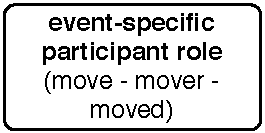
\includegraphics[scale=0.6]{chap-introduction/figs/stage1}}
    \caption[Formation\is{formation} of case markers: stage II]{In the first stage, the experiments start with a lexicon but without any grammar. The lexicon may contain words such as {\em move}, whose event structure may include participant roles such as `mover' (i.e. the one who did the moving) and `moved' (i.e. the thing that is being moved). However, the language has no means of marking those participant roles explicitly, hence the hearer has to infer the intended interpretation from the context.}
      \label{f:stage1}
\end{figure}

The experiments in this book therefore start from the point where a population of language users have already evolved a lexicon, but {\bfseries no grammar yet} (see Figure \ref{f:stage1}). This point of departure is not only justified by the empirical observation that new case markers evolve from existing lexical items (see further below), but also by the fact that experiments on artificial language evolution have already shown how vocabularies may emerge in a population of grounded embodied agents \citep[e.g.][]{steels96emergent, steels96selforganizing, steels97selforganizing}. In this way we can better isolate the features that are hypothesized to be formed in the experiments. Of course, once the dynamics of these experiments are better understood, a series of integrated experiments must be carried out to confirm the results.

\subsection{Stage II: specific marking}
\label{s:stage2}

Attested examples of the emergence\is{emergence} of modern case marker\is{case!case marking}s show that they are recruited from existing lexical items and that they start out in very restricted use scenarios. \citet[chapter 6]{blake94case} gives examples of how verbs, noun\is{noun}s and even adverb\is{adverb}ial particles can develop into case marker\is{case!case marking}s. Blake writes that a predicate like COME is a two-place predicate implying a `comer' and a `destination'. A predicate like LEAVE mirrors this implication by having a `leaver' and a `source\is{semantic role!source}'. A predicate like FLY, however, only implies a `flier'. If speakers then wish to produce utterances such as {\em he flew to/from Bangkok}, pairs of predicates can be used. Blake gives the following examples from Thai\is{Thai}:

\eal
\label{e:thai}
\ex[]{
\gll th\^{a}n c\`{a} bin maa krungth\^{e}ep \\
he will fly come Bangkok \\
\glt `He will fly to Bangkok.'
}
\ex[]{
\gll th\^{a}n c\`{a} bin c\`{a}ak krungth\^{e}ep \\
he will fly leave Bangkok \\
\glt `He will fly from Bangkok.'
}
\hspace{0.2cm}\citep[163--164]{blake94case}
\zl

\begin{figure}[t]
\centerline{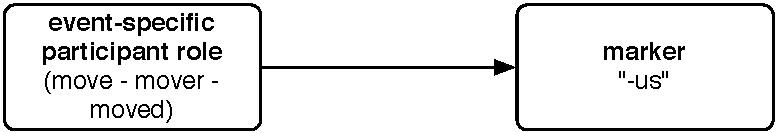
\includegraphics[scale=0.6]{chap-introduction/figs/stage2}}
  \caption[Formation\is{formation} of case markers: stage II]{In the second stage, a specific marker\is{case!case marking} arises in order to solve a communicative problem. In natural languages, this marker\is{case!case marking} is often a lexical item which is recruited for a new use. In the experiments, this stage involves the invention of a new marker\is{case!case marking}.}
   \label{f:stage2}
\end{figure}

Such languages are known as `serial verb language\is{serial verb} languages'. The second verb is (usually) non-finite\is{finiteness} and cannot be marked for tense\is{tense}, aspect\is{aspect} or mood\is{modality} independently of the first verb, and it takes no expressed subject\is{syntactic role!subject} or it implies the same subject\is{syntactic role!subject} as that of the first verb. Blake writes that functionally speaking, these second verbs are equivalent to preposition\is{preposition}s. Serial verb language\is{serial verb language\is{serial verb}} constructions are in fact very frequent and their development into adposition\is{adposition}s and case marker\is{case!case marking}s has been widely attested, especially in the languages of West Africa, New Guinea, Southeast Asia and Oceania (ibid., at 163; also see \citealp{givon97introduction}, section 7, for more on serial verb language\is{serial verb} constructions and similar examples).

The recruitment and evolution\is{evolution!cultural evolution} of a lexical item into an adposition\is{adposition} and eventually a case marker\is{case!case marking} is a long and complex process. For reasons that I will explain later on in this book, this crucial step in grammaticalization\is{grammaticalization} is `scaffold\is{scaffold}ed' in the experiments. Rather than reusing\is{reuse} an existing lexical item in a more grammatical way, the artificial agents will be capable of inventing a new form which already acts as some kind of adposition\is{adposition} or verb-specific case marker\is{case!case marking}, as shown in Figure \ref{f:stage2}. The experiments thus simplify stage II in order to focus first on the function of such marker\is{case!case marking}s and how they can be propagat\is{propagation}ed in a speech community\is{speech population}. It is needless to say, however, that this part of the grammaticalization\is{grammaticalization} chain remains on the research agenda for future experiments and first steps towards grammaticalization\is{grammaticalization} of existing lexical elements have already been taken by \citet{wellens08flexible}.

\subsection{Stage III: semantic role\is{semantic role}s}
\label{s:stage3}

When verb-specific case markers propagate successfully in a speech community, they often extend their coverage to other verbs as well. To come back to example \ref{e:thai}, this would mean that {\em maa} `come' evolves from the marker\is{case!case marking} of the destination of a flight to a general allative\is{case!allative} case role (i.e. the destination of motion events). Extension of the use of a marker\is{case!case marking} would in this case be {\em semantically motivat\is{semantic motivation}ed} and can occur by analog\is{analogy}ical reasoning over events. This is also the strategy that is employed in the experiments. 

Figure \ref{f:stage3} illustrates the new mapping between meaning and form when case markers become generalized semantic markers. Instead of directly mapping a particular participant role (e.g. the `mover') onto a case marker, a {\bfseries semantic role} (such as Agent) mediates between this mapping.

Since case marker\is{case!case marking}s in natural languages usually carry more than one function, it is hard to say what the semantic role\is{semantic role}s are that underlie a syntactic pattern. We can however look at `agnating structures' \citep{gleason65linguistics}. Agnation\is{agnation} illustrates a structural relationship between two grammatical constructions which have the same (major) lexical items, but different syntactic structures. If the alternation between these two structures is recurrent for groups of constructions, then this can be seen as a pattern in the language. An example of agnating\is{agnation} structures is the alternation between the English\is{English} ditransitive\is{ditransitive clause} (as in {\em I gave him a book}) and its preposition\is{preposition}al counterpart (as in {\em I gave the book to him}). 

Differences in the semantic categorization of verbs can come to surface if small but regular variation\is{variation}s show up between these agnating\is{agnation} structures. Compare the groups of agnating\is{agnation} structures in the following examples:

\begin{figure}[t]
\centerline{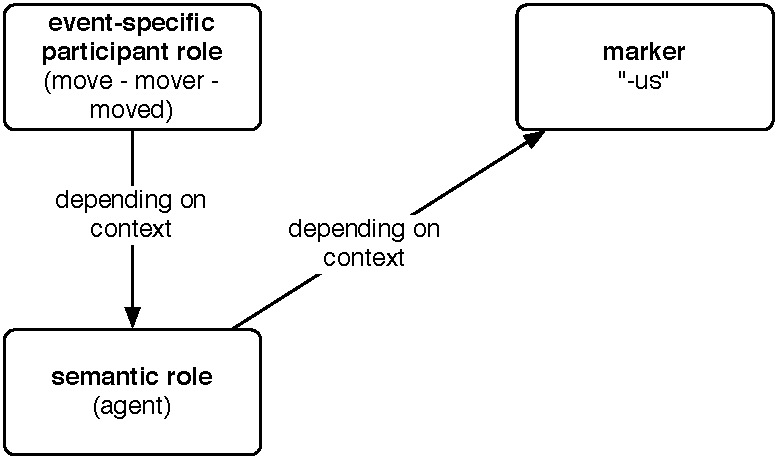
\includegraphics[scale=0.6]{chap-introduction/figs/stage3}}
  \caption[Formation\is{formation} of case markers: stage III]{Specific marker\is{case!case marking}s may get exten\is{extension}ded through analog\is{analogy}y in stage III. They now start to act as semantic role\is{semantic role}s.}
   \label{f:stage3}
\end{figure}

\ea
\label{e:agnate1}
\begin{tabbing}
I gave him a book. \hspace{2cm} \= I gave the book to him.
\\ I sent him a letter. \> I sent the letter to him.
\end{tabbing}
\z
\ea
\label{e:agnate2}
\begin{tabbing}
I baked him a cake. \hspace{1,85cm} \= I baked a cake for you.
\\I bought him a present. \> I bought a present for him.
\end{tabbing}
\z

Both groups of verbs can occur in the ditransitive\is{ditransitive clause} construction, but they select a different preposition\is{preposition} in the agnating\is{agnation} preposition\is{preposition}al construction. The choice for either {\em to} or {\em for} is semantically motivat\is{semantic motivation}ed: the verbs listed in example \ref{e:agnate1} entail\is{entailment} an {\em actual} transfer of the direct object\is{syntactic role!object} (= recipient), whereas the verbs in example \ref{e:agnate2} indicate that there is an {\em intended} transfer (= beneficiary). This is confirmed in the fact that sentences such as {\em ?I gave him a book, but he refused it} feel awkward, whereas sentences such as {\em I baked him a cake, but he refused it} are perfectly acceptab\is{acceptability}le. So it seems that both groups of verbs belong to different subclasses.

The exten\is{extension}sion of specific marker\is{case!case marking}s to semantic role\is{semantic role}s is useful for communication in several ways. First of all, semantic role\is{semantic role}s increase the potential for generalization in a language: by exten\is{extension}ding the functionality of a semantic role\is{semantic role}, there is a higher chance that it will be reuse\is{reuse}d for categorizing new and similar participant role\is{participant role}s as well. Instead of having to negotiat\is{negotiation}e a different marker\is{case!case marking} for each new instance, speakers of a language can thus make a semantically motivat\is{semantic motivation}ed innovat\is{innovation}ion which increases the chance that the hearer will understand the speaker's intention. Second, and related to the first point, semantic role\is{semantic role}s increase the expressiveness\is{expressiveness} of a language because they allow speakers to profile different aspects of the same event. For example, semantic role\is{semantic role}s can focus on the relation between an agent\is{semantic role!agent} and a patient\is{semantic role!patient} as in {\em he broke the window}, but also profile exclusively the resulting state\is{aspect!state} of one of the participants as in {\em the window was broken}. Finally, semantic role\is{semantic role}s can significantly reduce the inventory size by grouping together larger classes of verbs.

The model proposed in this book predicts that the convention\is{convention}alization of a mapping between verb-specific arguments and semantic role\is{semantic role}s (even though semantically motivat\is{semantic motivation}ed) is neither a determined nor a straightforward one. The choice depends on the convention\is{convention}s that are already present in the language, on a speaker's previous experience, frequency\is{frequency}, etc. Moreover, the model predicts that there will be several varieties in the population\is{speech population} which compete with each other for becoming the dominant semantic role\is{semantic role} of a particular argument. Thus we can expect that languages come up with very divergent classifications. For example, Italian\is{Italian} features dative\is{case!dative} subject\is{syntactic role!subject}s with verbs such as {\em like} \citep[27]{palmer94grammatical}, whereas English doesn't:

\ea
\gll Gli piacciono le ciliege \\
they.{\dat} like \textsc{det} cherries \\
\glt `They like cherries.'  \\
\z


Linking similar events can also be reversed from language to language. For example, when French\is{French} speakers want to say {\em I miss you}, they literally say something like `you are missing to me':

\ea
\gll Tu me manque-s. \\
you me miss-2{\sg}.{\prs} \\
\glt `I miss you.' \\
\z


So semantic role\is{semantic role}s seem to be language-specific, which fits our assumption\is{assumption} that they have to be constructed and learned. But once they become part of a language, are they an affair of `take it or leave it', or is it possible that the same verb-specific participant role\is{participant role} can be mapped onto multiple semantic role\is{semantic role}s? The answer seems to be that this mapping too is indirect and dependent on the context. For example, the `sneezer' in {\em he sneezes} seems to be a patient\is{semantic role!patient}, whereas it is (also) a causer\is{semantic role!causer} in {\em he sneezed the napkin off the table}. All the above observations are reflected in Figure \ref{f:stage3} and more evidence is provided in the next chapter.

\subsection{Stage IV: syntactic role\is{syntactic role}s}
\label{s:stage4}

\begin{figure}[t]
\centerline{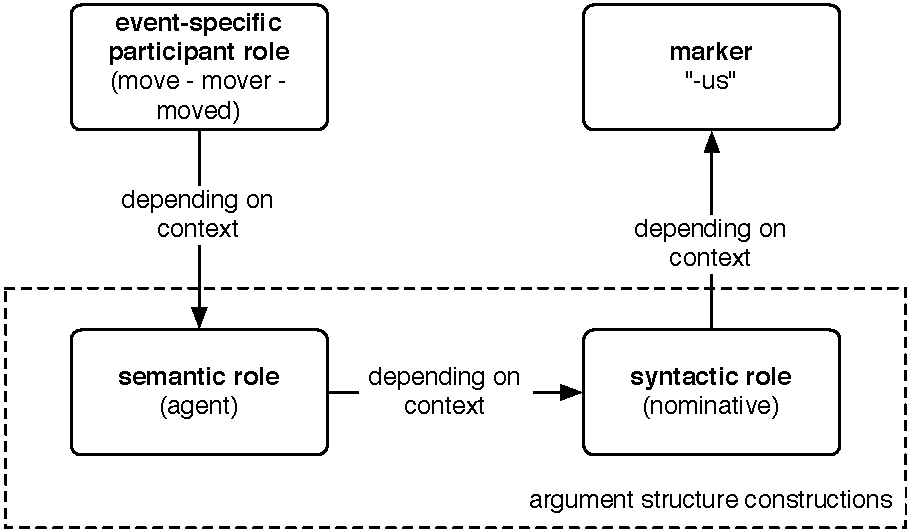
\includegraphics[scale=0.6]{chap-introduction/figs/case-quadrant}}
  \caption[Formation\is{formation} of case markers: stage IV]{In the next step, even more abstraction\is{abstraction}s occur through syntactic role\is{syntactic role}s. The mapping between semantic role\is{semantic role}s and grammatical cases is hypothesized to be handled by \is{event structure}\is{construction!argument structure construction}argument structure constructions which can combine several semantic role\is{semantic role}s into a larger pattern.}
   \label{f:stage4}
\end{figure}

Languages typically have thousands of verbs and semantic roles. However, case languages tend to have streamlined case systems with only a dozen cases or less. As \citet{croft91syntactic} states, {\em ``surface case marking\is{case!case marking} imposes structure on thematic relations to an even more abstract degree than verb roots impose structure on the human experience of events''} (p. 158--159). We know that a case marker has evolved into a {\em syntactic} marker once it can be dissociated from a particular semantic role \citep[2--3]{givon97introduction}. For instance, the German nominative case can be used for covering virtually all semantic roles of the language. 

Figure \ref{f:stage4} shows an updated mapping between event structure meaning and its surface form, which is now mediated by an abstract and hidden layer of semantic and syntactic categories. I will from now on refer to this picture as the {\bfseries grammar square}. Each mapping in the square can vary according to the communicative and linguistic circumstances, so the relation between a participant role\is{participant role} and its morphosyntactic realization is multilayered and indirect.

The picture presented here however has the danger that case marker\is{case!case marking}s are considered in isolation, whereas they can only be understood in relation to the other parts of the pattern in which they occur. Indeed, the mapping of semantic role\is{semantic role}s onto syntactic role\is{syntactic role}s (and vice versa) is hypothesized to be taken care of by \is{event structure}\is{construction!argument structure construction}{\bfseries argument structure constructions} \citep{goldberg95construction}. These constructions may be schematic, verb-class-specific\is{construction!verb-class-specific construction} or even verb-specific. I will come back to this point in the next Chapters that introduce the formalization of such constructions.

\subsection{Further developments}
\label{s:case-markers}

Stages I--IV described the possible evolutionary pathway of a case marker\is{case!case marking} which resulted in an inflection\is{inflection}al category that groups together various semantically related roles. This is also the endpoint of the experiments described in this book because they focus only on case marking\is{case!case marking} as a way to express event structure\is{event structure} in a grammatical way. There are, however, other functions which may be performed by case marker\is{case!case marking}s such as packaging information structure\is{information structure}, marking perspectiv\is{linguistic perspective}ization and other grammatical distinctions such as gender\is{gender} and number\is{number} (as argued in section \ref{s:case-functions}). Especially information structure\is{information structure} seems to be the most important pressure for case marker\is{case!case marking}s to exten\is{extension}d their coverage and become even more dissociat\is{dissociation}ed from their previous meaning.

Finally, case marker\is{case!case marking}s eventually decline and even whole grammatical systems\is{case!case system} of case may get lost and replaced by other grammatical devices. This is apparent in the (almost) complete loss of case marking\is{case!case marking} in languages such as English\is{English}, French\is{French} and Dutch\is{Dutch}, which replaced it with word order\is{word order} constraints. Individual case marker\is{case!case marking}s may disappear because they are `merged' with another case such as the merger of the instrumental\is{case!instrumental} and locative\is{case!locative} case in Middle Indo-Aryan\is{Indo-Aryan} \citep[176]{blake94case}. Whereas merger seems to be relatively common in the life cycle of case systems\is{case!case system}, case split\is{case!case split} is quite rare. Merger of case marker\is{case!case marking}s means that the case system\is{case!case system} is reduced unless new members are recruited. With the loss of cases and further developments in the grammaticalization\is{grammaticalization} of case marker\is{case!case marking}s, the different cases of a language may become insufficiently differentiated from each other. This allows other strategies, such as word order\is{word order} complemented with preposition\is{preposition}s in English\is{English}, to become more popular and eventually the new convention\is{convention}s of a language. The decline of entrench\is{entrenchment}ed and convention\is{convention}alized grammatical units falls beyond the scope of this book.

\section{Modeling language evolution}
\label{s:models}

The experiments reported in this book are models of {\em artificial language evolution}, in which computational and mathematical models and robotic experiments are used for evolving (new) artificial languages that have similar properties as found in natural languages. As such, the methodology provides possible and operational explanations for those properties. Experiments typically involve a {\em population of artificial language users} (henceforth called {\em agents}) that engage with each other in communicative interactions. 

\subsection{Three models of artificial language evolution}

There is a wide consensus in the field that language has evolved because there is a {\em selectionist} system underlying it. Despite this consensus, there is disagreement on how linguistic variation and hence the potential for change is caused, and which selectionist pressures are operating to retain a particular variation in a language. There are basically three different perspectives based on genetic evolution, cultural transmission, and problem-solving respectively.

\begin{figure}[t]
\centerline{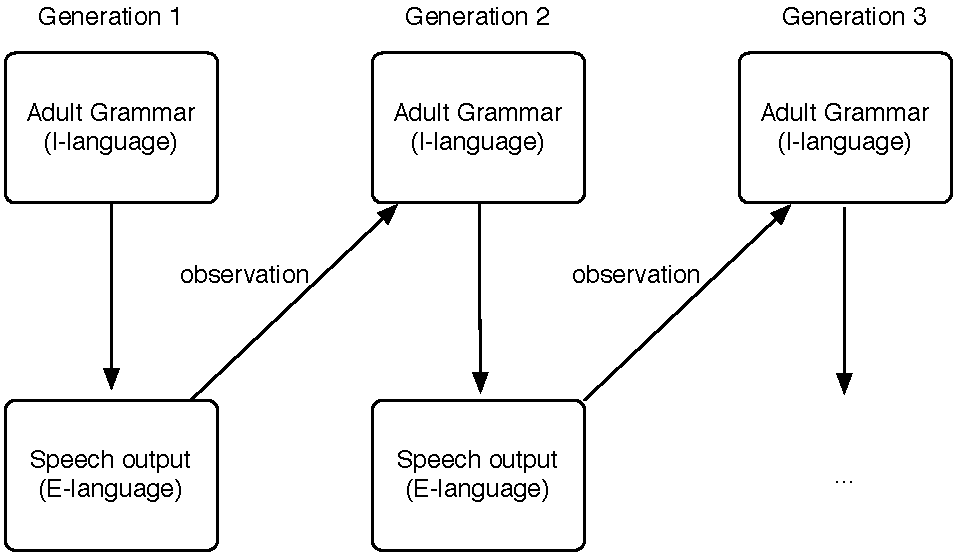
\includegraphics[scale=0.55]{chap-introduction/figs/childbased}}
  \caption[Child-based language change\is{language change}]{Iterated learning models assume that languages evolve because children are faced with a learning bottleneck when observing and reconstructing the language of the previous generation.}
   \label{f:child-based}
\end{figure}

Models of genetic evolution \citep[e.g.][]{briscoe00grammatical, nowak01evolution} investigate the biological evolution of the {\em language faculty} (i.e. our ability to acquire and use language). These models put the selectionist pressure at the level of fitness (i.e. the ability to survive and reproduce), which is assumed to be directly related to communicative success. Agents are endowed with an artificial genome that determines their communicative behavior. Depending on how much of language is assumed to be innate, the genome may include which concepts can be employed by the agents for structuring their world, which types of categories are to be used, and so on. Potential innovation takes place when this genome is transmitted from parents to children. Because genome copying involves crossover\is{crossover} and possibly mutation\is{mutation}, variation\is{variation} is inevitable, and some of it will lead to higher or lower success.

Iterated Learning Models \citep[ILM\is{Iterated Learning Model (ILM)},][]{brighton05cultural, kirby01spontaneous, kirby02emergence, kirby04from, smith03iterated} investigate what happens when language is culturally transmitted from one generation to the next without any interference from functional pressures, as illustrated in Figure \ref{f:child-based}. Each cycle, an adult generation (typically represented by a single agent) produces speech output based on its internal grammar, which is observed by a new generation (also typically a single agent) for reconstructing the language. The model assumes that there is a learning bottleneck (i.e. the child cannot observe all utterances in the language), hence the learner agent may overgeneralize the input based on innate learning biases. When the adult agent `dies' and is replaced by the child, the mistakes in learning become the new convention and the language changes. The ILM shows strong affinity for child-based theories of language change as found in generative linguistics \citep{king69historical}.

The third class of models views the task of building and negotiat\is{negotiation}ing a communication system as a kind of problem-solving\is{problem-solving} process. Agents try to achieve a communicative goal with maximal success and minimal effort. This problem-solving\is{problem-solving} process is definitely not a rational but an intuitive one that is seldom accessible to conscious inspection. It is not an individualistic problem-solving\is{problem-solving} process either, but a collective one, in which different individuals participate as peers. According to this view a communication system is built up in a step by step fashion driven by needs and failures in communication, and it employs a large battery of strategies and cognitive mechanisms which are not specific to language but appear in many other kinds of cognitive tasks, such as tool design\is{tool design} or navigation\is{navigation}. Recent experiments by \citet{galantucci05experimental} on the emergence\is{emergence} of communication in human subject\is{syntactic role!subject}s provide good illustrations of these problem-solving\is{problem-solving} processes in action. Variation and innovat\is{innovation}ion in problem-solving\is{problem-solving} models are common because each individual not only tries to converge to the shared communication system, but can also contribute innovat\is{innovation}ions to it. In fact the main challenge is rather to explain how agreement between individuals and thus a globally shared population\is{speech population} language can ever arise. This approach to language evolution\is{evolution!cultural evolution} is closely related to cognitive-functional\is{cognitive-functional approach} theories of language and utterance-based\is{selection!utterance-based selection} models of linguistic change \citep{croft00explaining, croft05relevance}.

The three models are of course not mutually exclusive: it is clear that the models of cultural evolution\is{evolution!cultural evolution} expect a rich cognitive-linguistic system, which can only be explained through the genetic endowment of the agents. Similarly, problem-solving\is{problem-solving} models can be modeled using a generation turnover as well \citep{vogt07group}. However, one particular advantage of the problem-solving approach is that it attempts to explain as many linguistic phenomena as possible in terms of functional and communicative pressures. This means that innate mechanisms are only used as a last resort, which arguably avoids putting all the explanatory burden on the shoulders of biology. This book therefore subscribes to the problem-solving approach.


\subsection{The do's and don'ts of artificial language evolution\is{artificial language evolution}}
\label{s:methodology}

The question of the origins and evolution of language is notoriously difficult because there are no fossil traces or written accounts left of the first languages, and there are no data available about the biological changes that enabled language. These facts have led \citet{kirby03language} to pose the provocative question: is language evolution\is{evolution!cultural evolution} the hardest problem in science?

Without attempting to answer that question, it actually {\em is} possible to come up with solid theories despite the lack of real-life data: in various other disciplines, such as the origins\is{origins} of the universe, significant advances are made using mathematical models and computational simulations. Another example is Artificial Life\is{Artificial Life} where computational models, robot\is{robot}ic experiments and biochemistry are used as techniques to develop artificial phenomena that may help to explain processes of evolution in natural phenomena.

{\bfseries (i) Creating natural language-like phenomena.} Let me start by debunking a myth about modeling language evolution that seems to be lingering in the minds of some people: computational simulations and robot\is{robot}ic experiments can never lead to the emergence\is{emergence} of an actual natural language like English\is{English} or Russian\is{Russian}. There are just too many factors that have shaped these languages and modeling them would require to model the entire state of every speaker and every interaction {\em ever}. The `languages' that emerge in this kind of experiments should thus not be {\em directly} linked to natural languages: they are novel artificial constructs and hence {\bfseries the methodology only offers a `proof of concept' of what results can be achieved within the specific set-up of a given experiment}. However, these constructs may be natural language{\em -like} and thus offer a possible and working hypothesis for how similar phenomena could have come about in natural languages.

Secondly, even in abstraction, we cannot model every aspect of language at once, just as it is impossible to perform controlled psycholinguistic experiments that take every detail about language processing into account. The key is therefore to pick a phenomenon observed in natural languages and try to isolate this feature into a controlled simulation or experiment. Focusing on smaller problems is standard practice in many scientific disciplines. As Stephen Hawkin writes in his {\em A Brief History of Time}:

\begin{quote}
It turns out to be very difficult to devise a theory of the universe all in one go. Instead, we break the problem up into bits and invent a number of partial theories. Each of these partial theories describes and predicts a certain limited class of observations, neglecting the effects of other quantities, or representing them by simple sets of numbers. It may be that this approach is completely wrong. If everything in the universe depends on everything else in a fundamental way, it might be impossible to get close to a full solution by investigating parts of the problem in isolation. Nevertheless, it is certainly the way we have made progress in the past. 
\\ \cite[12]{hawkin88brief}
\end{quote}

In problem-solving models of artificial language evolution\is{artificial language evolution}, the researcher therefore first chooses a topic of interest that is common to most if not all languages, such as tense\is{tense}, aspect\is{aspect} and mood\is{modality}. Investigating such a feature involves the following steps \citep{steels06how}:

\begin{enumerate}
\item The researcher selects a feature of language to investigate;
\item The researcher hypothesizes which set of cognitive mechanisms and external pressures are necessary for the emergence\is{emergence} of this feature:
\begin{enumerate}
\item These cognitive mechanisms are operationalized in the form of computational processes, and a population\is{speech population} of simulated or embodied agents is endowed with these mechanisms;
\item The external pressures are operationalized in the form of an interaction pattern embedded in a simulated or real world environment;
\end{enumerate}
\item Systematic computer simulations are performed demonstrating the impact of the proposed mechanisms. If possible, results should be compared between simulations {\em with} a proposed mechanism and simulations {\em without} this mechanism in order to show that it is not only a sufficient but also a necessary prerequisite for the emergent feature. 
\end{enumerate}

Even if the simulations show that the investigated feature only emerges if certain mechanisms are included, this still does not prove anything about similar features in natural languages because different evolutionary pathways are possible. However, the simulations then at least show one possibility and may provide an additional piece of the puzzle next to evidence from linguistics, archeology, biology and other fields.

{\bfseries (ii) Clarifying the scaffold\is{scaffold}s and assumption\is{assumption}s.} Computational simulations and robot\is{robot}ic experiments are at the same time blessed and cursed with the fact that every detail of the hypothesis has to be spelled out completely, otherwise the system does not work. `Blessed' because this may reveal effects of the hypothesis that were overlooked or not expected by the verb\is{verb}al theory; `cursed' because there is a danger of `kludging' something together to get the system off the ground. There is often a fine border between significant results and quirks resulting from a kludge, so it is crucial that it is crystal clear which features of the model are supposed to be `emergent' on the one hand, and which features are `assumed' or `scaffold\is{scaffold}ed' on the other.

Assumptions and scaffold\is{scaffold}s are unavoidable in computational simulations because it is simply impossible to explain everything at once. Drawing the line between what is `assumed' and what is `scaffold\is{scaffold}ed' is not always an easy decision. I define `assumed features' as those aspects of the simulations that we cannot explain using the methodology described here. One example is the assumption\is{assumption} that agents are social and cooperative beings that {\em want} to reach communicative success\is{communicative success}. Another example is the capacity for building composite structures. I define `scaffold\is{scaffold}ed features' as those aspects of the simulations that in principle could be evolved using the methodology but are given so that not every simulation or experiment has to start from scratch. An example of a scaffold\is{scaffold} is the space of possible phonemes: in none of the experiments in this book, agents had to learn the distinctive sounds of their language. These `scaffold\is{scaffold}ed' features may be brought in at a later stage or form the subject of other experiments, such as work on the emergence\is{emergence} of vowel systems\is{vowel systems} \citep{deboer00self, oudeyer05self-organization}.

{\bfseries (iii) Global versus local measure\is{measure!local measure}s.}
Another important dichotomy is that of global versus local measure\is{measure!local measure}s. In experiments that study language from a usage-based point-of-view, only local measure\is{measure!local measure}s which can be observed by the agents themselves within the local interaction may have an influence on the linguistic behaviour of the agents. Typical local measure\is{measure!local measure}s are:

\begin{itemize}
\item Success of the language game\is{language game}: the agents that are involved in a language game\is{language game} can experience whether the game was a success or not. This may influence the confidence\is{confidence} with which they employ certain linguistic items;
\item Search and difficulty: An agent can `measure' for example the ambiguity\is{ambiguity} of an utterance because it causes an elaborate search space during processing;
\item Cognitive effort\is{cognitive effort}: Agents can `measure' the cognitive effort\is{cognitive effort} needed during parsing and production, such as how much processing time they need, how many times they need to add information from their world model to the linguistic data, how many times they need to perform additional operations such as egocentric perspective\is{egocentric perspective transformation} reversal, etc.
\end{itemize}

Global measures, then, are measures which are used by the experimenter solely for analyzing the simulations. These measures should by no means have an influence on the linguistic behaviour of the agents. For example, if an agent should decide between two competing forms for a meaning, it has to make the appropriate choice based on its {\em individual} past experiences and on the local information in the language game\is{language game}. A global measure\is{measure!global measure} such as how many agents share one of the competit\is{competition}ors would require an overview of the complete population\is{speech population}, which no speaker ever has. Convergence has to come about in a distributed, self-organiz\is{self-organization}ed fashion without external guidance or central control.

\section{A brief history of prior work}
\label{s:history-of-research}

This book is part of more than a decade worth of research on language as a complex adaptive system\is{complex adaptive system}. The research itself is rooted in prior work in Artificial Intelligence\is{Artificial Intelligence} and robot\is{robot}ics in the mid-eighties, which involved home-made robot\is{robot}s of all shapes and sizes -- driving around on wheels, flying with balloons and propellers, or waggling their tails in the rough waters of the Brussels' university swimming pool. These creations were the result of a break with mainstream research in Artificial Intelligence\is{Artificial Intelligence}: whereas most work in AI tried to formalize human intelligence, Luc Steels and his students at the Artificial Intelligence Laboratory (VUB, Brussels) investigated how `intelligence' might evolve in a community of physical agents as they autonomously interact with each other, their environment, and humans. They thus developed a bottom-up, behaviour-oriented approach to sensori-motor intelligence, which was at the same time also being explored by Rodney Brooks at the MIT Artificial Intelligence Lab \citep{steels95alife-route}.

Even though fascinating results were obtained, something was missing that could ever lead the experiments to other, more human-like intelligent behaviour than was displayed by the robot\is{robot}s. The research then shifted its focus from beha-viour-based robot\is{robot}ics to embodied language in the autumn of 1995 when Steels had the following two ideas: first of all, language may have been the missing link in the initial experiments. Language may be a necessary step that enables the human cognitive system to bootstrap itself in tight interaction with the world and in a population\is{speech population} of social cooperative agents \citep{steels03intelligence}. Second, the same principles and mechanisms that had since 1985 proven to be relevant for the work in robot\is{robot}ics also had to be relevant for bootstrapping intelligence and language. These principles included self-organization, structural coupling\is{structural coupling}, level formation\is{level formation}\is{formation} and other (mainly biologically inspired) mechanisms \citep{steels97synthesising}. In this section I will give an overview of the research efforts at the AI Lab in Brussels and SONY Computer Science Laboratory Paris (which adopted the work on language as one of its founding research topics in 1996).

\subsection{The emergence of adaptive lexicons}
\label{s:history-lex}

The first breakthrough experiment investigated how self-organization could explain the emergence of coordinated vocabularies \citep{steels97selforganizing}. Self-organi-zation is a phenomenon in which coupled dynamical systems form a structure of increased complexity without guidance by an outside source or some central controller. Standard examples of self-organization are the formation\is{formation}s of termite nests or paths in an ant society. The process has been used successfully for describing phenomena in various scientific disciplines: physics (e.g. crystalization\is{crystalization}), chemistry (e.g. molecular self-assembly\is{molecular self-assembly}), economy (catallaxy\is{catallaxy}), etc. Language is also an example of a complex system that is shared by a speech community\is{speech population} without central control (although some `watchdogs' such as the {\em Acad\'{e}mie fran\c{c}aise\is{Acad\'{e}mie fran\c{c}aise}} do their utter best to have people speak according to their set of standards). 

In the experiments reported by \citet{steels97selforganizing}, agents engage in communicative interactions about a set of predefined meanings. If the speaker has no word for a meaning, he will invent a new one which may be adopted by the hearer. The agents assign a {\bfseries success score} to the form-meaning mappings based on success in the interaction. After some rounds of negotiat\is{negotiation}ion, a shared set of form-meaning mappings emerges without the need for central control. Similar experiments using neural network\is{neural network}s were reported by \citet{batali98computational}.

The notion of a {\bfseries language game\is{language game}} was first introduced by Steels (\citeyear{steels96selforganizing}; also see Steels \citeyear{steels01language} for an introduction). Language games are routinized local interactions or scripts. An example of a language game\is{language game} in natural languages is a speaker who asks {\em Can you pass me the salt, please?}. The language game\is{language game} is a success if the hearer passes the salt or even if he responds that he refuses to do so (but at least he understood the message). The game is a failure if the hearer passes the pepper instead of the salt or if he just shrugs her shoulders. The speaker can then point to the salt, which gives the hearer some additional clues as to what he meant with {\em salt}. An iteration of language game\is{language game}s is called a {\bfseries dialogue\is{dialogue}}, but this more complex interaction pattern has not been studied anymore since \citet{steels96selforganizing}. 

In these first experiments, the meaning space of the agents was predefined. However, since no concepts or categories are assumed to be innate in this line of work, several experiments have been conducted investigating how agents can create their own concepts and meanings. The first breakthrough was reported in \citet{steels96perceptually}, in which agents created perceptual categories through {\bfseries discrimination game\is{discrimination game}s}. In a discrimination game\is{discrimination game}, an agent tries to discriminate a certain object from the other objects in the context by creating or using a set of one or more distinctive features for that object. In the next breakthrough experiment, discrimination game\is{discrimination game}s and language game\is{language game}s were coupled to each other so that agents did not only self-organiz\is{self-organization}e a lexicon\is{lexicon}, but also used the lexicon\is{lexicon} for sharing concepts or perceptual distinctions \citep{steels97constructing, steels97origins-ontologies, steels98structural, steels99how, steels99spontaneous}. In a next step, it was shown how these ideas can be grounded in actual robot\is{robot}ic agents \citep{steels01role, steels02grounding, steels97grounding, vogt00lexicon}. The structural coupling\is{structural coupling} of concepts and lexicon\is{lexicon}s has also been successfully applied to the domains of colour\is{colour} \citep{belpaeme02factors, belpaeme05colourful, steels05coordinating} and space \citep{loetzsch08typological, steels08perspective-alignment}.

The research on lexicon\is{lexicon} emergence\is{emergence} steadily grew and touched upon topics such as how lexicon\is{lexicon}s can continue to change and evolve because of language contact\is{language contact} and population\is{speech population} dynamics \citep{steels97language-learning, steels99spatially} and stochasticity\is{stochasticity} in cultural transmission \is{transmission}\citep{kaplan98architecture, steels98spontaneous, steels98stochasticity}. The experimenters also developed the notion of a {\bfseries semiotic landscape\is{semiotic landscape}}, a powerful framework to study the {\bfseries semiotic dynamics\is{semiotic dynamics}} involved in the language game\is{language game}s \citep{steels99collective, steels99situated}. The research culminated in the Talking Heads\is{Talking Heads experiment} experiment which involved thousands of agents travelling over the internet in order to play language game\is{language game}s with each other \citep{steels99talking-heads, steels00puzzle, steels01language, steels99collective, steels99situated, steels02bootstrapping, steels02crucial}.

The research on lexicon\is{lexicon} emergence\is{emergence} is still being pursued today. For example, the Naming Game\is{language game!naming game}, which first appeared in \citet{steels97selforganizing}, has recently been implemented in humanoid robot\is{robot}s that autonomously have to recognize objects as individuals and then agree on names for them. The Naming Game\is{language game!naming game} has also been picked up by scientists from statistical physics and complex systems who search for scaling laws and who investigate the long-term behaviour of the system using mathematical models \citep{baronchelli06sharp, devylder07evolution}. Other recent work using computational modeling investigates how word meanings can be more flexible and how the emergence\is{emergence} of lexicon\is{lexicon}s can scale up to much larger worlds \citep{wellens08flexible}.

\subsection{Towards grammar}
\label{s:towards-grammar}

Even though the first decade has been largely spent on investigating the properties of emergent adaptive lexicon\is{lexicon}s, the emergence\is{emergence} of grammar has always been on the research agenda with first attempts as early as 1997 \citep{steels97origins-syntax}. The research strategy involves moving all the insights gained from the experiments on lexical languages to the domain of grammar and identify which additional mechanisms and ideas are needed for the emergence\is{emergence} of languages featuring grammatical properties \citep{steels05emergence}.

The first steps towards grammar involved a pregrammatical stage of {\bfseries multiple word utterances\is{multiple word utterances}}, which was first investigated by \citet{steels96emergent}. In this experiment, multiple word utterances\is{multiple word utterances} emerge naturally as the set of distinctive features for talking about objects expands and the agents have to adapt to cope with it. \citet{vanlooveren05design} then showed how a multiword naming game\is{language game!multiword naming game} can yield a more efficient communication system because a smaller lexicon\is{lexicon} could be used for naming objects. However, none of these experiments involved any grammar.

At the end of the nineties, a significant breakthrough was achieved which resulted in the general roadmap for investigating the emergence\is{emergence} of grammar that is still being followed today (\citealp{steels99talking-heads}: 44--47; \citealp{steels00emergence}). Whereas lexical languages are perfectly suited for language game\is{language game}s involving only one object, grammar becomes useful when agents have the possibility of communicating about multiple objects because the search space becomes exponentially larger. Grammar thus emerges not in order to reduce inventory size or to become more learnable (as is proposed by genetic and Iterated Learning Models), but rather to {\bfseries reduce the complexity of semantic parsing} for the hearer \citep[this idea has been formalized and operationalized by][]{steels05what}. Luc Steels then worked on systems for studying the emergence\is{emergence} of {\bfseries compositional meanings} (see section \ref{s:other}) and for the emergence\is{emergence} of grammar to take care of these compositional meanings.

\citet{vanlooveren05design} applied these ideas to his experiments on multiple word games and lifted the agents' assumption\is{assumption} that multiple words always refer to the same object. For example, the utterance {\em yellow ball} might refer to one object (a yellow ball) or at least two objects (some yellow thing and a ball). When faced with this referential uncertainty\is{referential uncertainty}, the agents can exploit a simple syntax for indicating to the hearer which words refer to the same object. Referential uncertainty\is{referential uncertainty} has also been investigated from the viewpoint of pattern formation\is{formation}\is{pattern formation} \citep[as another pregrammatical stage,][]{steels07multilevel} and as a trigger for introducing additional syntax \citep{steels06how-grammar}.

Another key issue in the emergence\is{emergence} of grammar is the question of how agents can autonomously detect when additional constraints or grammar might become useful in order to improve their communicative success\is{communicative success}. The answer is `re-entran-ce\is{re-entrance}' \citep{steels03language}, a strategy which was already present in the experiments on the emergence\is{emergence} of lexicon\is{lexicon}s but which had to be developed further to fit into a grammatical framework. Re-entrance\is{re-entrance} can be seen as some kind of self-monitoring\is{monitoring} in which the speaker first simulates the effect of his utterance on the hearer by taking himself as a model. If he detects problems such as ambiguity\is{ambiguity} or an explosion of the search space during parsing, he will adapt his linguistic behaviour by adding more constraints or choosing a different verb\is{verb}alization. Similarly, the hearer can perform re-entrance\is{re-entrance} for learning novelties in the speaker's utterance. A similar mechanism called `the obverter strategy' can be found in other negotiat\is{negotiation}ion-based models as well \citep{smith03intelligent}. Another way to increase the autonomy of the agents is to offer them strategies for self-assessing what kind of communicative goals they can attain given their present linguistic experience \citep[called the `autotelic principle\is{autotelic principle}',][]{steels04architecture, steels04autotelic, steels07scaffolding}.

Most of the above ideas were put to practice in 2001 in the first `case experiment', which I will describe in Chapter \ref{c:base} and of which some results were published in \citet{steels04constructivist} and to a lesser extent in \citet{steels03language, steels07recruitment}. Luc Steels implemented a unification\is{unification}-based grammar formalism to support the experiment, which ultimately led to the first design of Fluid Construction Grammar\is{construction grammar!Fluid Construction Grammar} (FCG\is{construction grammar!Fluid Construction Grammar}, also see Chapter \ref{c:ar}). FCG\is{construction grammar!Fluid Construction Grammar} is under constant development to meet the demands and requirements of new experiments such as the following:

\begin{itemize}
\item A bidirectional\is{bidirectionality} and uniform way of language processing \citep{steels06unify}. This feature is needed for allowing agents to act both as a speaker and as a hearer; and for allowing the agents to perform re-entrance\is{re-entrance};
\item A way to deal with compositional semantics and to link meanings to each other \citep{steels05linking}.
\end{itemize}

The name `Fluid Construction Grammar\is{construction grammar!Fluid Construction Grammar}' comes from the fact that FCG\is{construction grammar!Fluid Construction Grammar} has many features in common with (vanilla)\is{construction grammar!vanilla construction grammar} construction grammar \citep{croft05logical} and that it aims at investigating the `fluidity' of language emergence\is{emergence} (i.e. various degrees of entrench\is{entrenchment}ment of linguistic units). A software implementation of FCG\is{construction grammar!Fluid Construction Grammar}, incorporated in a more general cognitive architecture called `Babel2', has been made freely available at {\em www.emergent-languages.org}.

Fluid Construction Grammar\is{construction grammar!Fluid Construction Grammar} has already been used for investigating the emergence\is{emergence} of compositionality \citep{debeule06emergence}, recursi\is{recursion}on and hierarchy\is{hierarchy} \citep{bleys08recursive, debeule07compositionality, debeule08emergence}, structures for expressing second-order\is{second-order semantics} meanings \citep{steels05planning} and semantic role\is{semantic role}s \citep{steels04constructivist, vantrijp08emergence}.

\subsection{Other research avenues}
\label{s:other}

The above account of the history of the research on language as a complex adaptive system\is{complex adaptive system} did not refer to the experiments on the emergence\is{emergence} of vowel systems\is{vowel systems} and phonology \citep{deboer00self, oudeyer05self-organization}. I also left out the work performed on event recognition\is{event recognition}, but I will come back to this in Chapter \ref{c:base}. Another area that I left largely uncovered is the research into conceptualization\is{conceptualization} and the emergence\is{emergence} of complex meanings.

Together with the key insights on the triggers and functions of grammar at the end of the ninetees, Steels developed a constraint-based system for studying the emergence\is{emergence} of compositional meaning \citep{steels00emergence} which uses constraint propagat\is{propagation}ion both for conceptualization\is{conceptualization} and interpretation. In the system, a set of constraints can be composed into some kind of semantic program that the speaker wants the hearer to perform. For example, if the speaker wants to draw the hearer's attention to a particular ball in the context, he has to conceptualize a network of meanings or constraints that will help the hearer to correctly identify this ball. For example, the utterance {\em the red ball} indicates to the hearer that he has to (a) filter the objects in the context and retain those that match with the prototype\is{prototype} [BALL], (b) filter this set of balls and retain the red ones, and (c) pick out the one remaining object (its uniqueness was indicated by the determiner\is{determiner} {\em the} in combination with the singular\is{number!singular} form {\em ball}). The system allows for the composition of second-order\is{second-order semantics} semantics (e.g. {\em the bigger ball}) and context-sensitive meanings (e.g. a `small' elephant is still bigger than a `big' mouse).

Even though at that time there was already an operational system, the research on compositional meanings was put on a hold to first develop a grammar formalism that could support it. With the recent advances in Fluid Construction Grammar\is{construction grammar!Fluid Construction Grammar}, the research got picked up again and first experiments have already been reported that couple meanings produced by the system to FCG\is{construction grammar!Fluid Construction Grammar} and vice versa \citep{bleys08recursive, steels05planning}. The system has also been completely re-implemented and improved upon \citep[see][for an introduction]{vandenbroeck07constraint, vandenbroeck08constraint}.

\setcounter{chapter}{1}
\chapter{Processing Case and Argument Structure}
\label{c:ar}

The mathematical properties of case and argument structure have been extensively studied in the tradition of formal grammars such as Combinatorial Categorial Grammar \citep[CCG;][]{steedman00syntactic}, Lexical-Functional Grammar \citep[LFG;][]{bresnan82mental} and Head-driven Phrase Structure Grammar \citep[HPSG;][]{sag94hpsg}. The focus of those studies has been the development of {\em competence models} (i.e. knowledge representations), thereby treating {\em linguistic processing} as a problem that can be dealt with separately. However, if our artificial agents have to use their linguistic knowledge in communicative interactions, we need a strong integration of both processing and competence.

One family of linguistic theories that is particularly interesting for achieving such an integration is {\em construction grammar}, because it is explicitly concerned with how meanings can be mapped onto forms and vice versa. Unfortunately, {\em computational} construction grammars are scarcely out of the egg: the formalizations of Construction Grammar \citep[CxG;][]{kay99grammatical} and Sign-Based Construction Grammar \citep[SBCG;][]{boas13sbcg} have not actually been implemented (yet), and Embodied Construction Grammar \citep[ECG\is{Embodied Construction Grammar},][]{bergen05embodied} only has a parsing model but cannot handle production.

In order to conduct the experiments presented in this book, I therefore implemented a bidirectional processing model for argument structure and case in Fluid Construction Grammar (FCG). To the best of my knowledge, this implementation is the first (and currently the only) constructional account of argument structure that handles both parsing and production. This Chapter discusses the operationalization in more detail, which is necessary for appreciating the structures that the artificial agents evolve in the experiments. I will discuss the operationalization's relevance for linguistic theory in more detail in Chapter \ref{c:impact-linguistics}, where I compare my solution to a recent proposal on argument realization in Sign-Based Construction Grammar. 

\section{Representing and linking meanings}
\label{s:linking}

The operationalization follows a proposal by Steels (\citeyear{steels05what}; also see \cite{debeule07compositionality, steels05linking, steels06how-grammar}) and uses a logic-based representation for meaning. For example, the utterance {\em box and ball} may be represented as follows:

\ea
box(?obj-x) $\wedge$ ball(?obj-y)
\z

As is standard practice in first order predicate calculus, variables (i.e. all symbols that start with a question mark) are used for referring to objects. The variable `?obj-x' thus has to be bound to the object [BOX] and the variable `?obj-y' has to be bound to the object [BALL]. Suppose that we want to say that the box is big and that the ball is blue, then the meaning may be represented as:

\ea
\label{m:expressed}
big(?obj-x) $\wedge$ box(?obj-x) $\wedge$ blue(?obj-y) $\wedge$ ball(?obj-y)
\z

Note that `big' and `box' share the same variable `?obj-x' because they both refer to the same object; and that `blue' and `ball' also share the same variable `?obj-y' because they both refer to [BALL]. The speaker may then express this meaning as {\em (the) big box and (the) blue ball}. Now imagine that the hearer is a non-native-speaker of English\is{English} who has learned several words, but hasn't acquired the grammar yet. In other words, he does not know that English\is{English} uses word order\is{word order} in an Adjective-Noun Construction\is{construction!adjective-noun construction} to indicate which adjective modifies which noun\is{noun}. If he just uses his limited linguistic knowledge of English, he would come up with the following parsed meaning:

\ea
\label{m:unexpressed}
big(?obj-w) $\wedge$ box(?obj-x) $\wedge$ blue(?obj-y) $\wedge$ ball(?obj-z)
\z

In this parsed meaning, there are neither shared variables between {\em big} and {\em box}, nor between {\em blue} and {\em ball} because lexical meanings do not specify which words go together. So there may be several hypotheses possible: each word may refer to a different object (i.e. in some languages adjectives can be used as heads of a phrase as well as noun\is{noun}s), {\em blue} may refer to [BALL] but also to [BOX] (as it is possible to put adjectives in French\is{French} both before and after a noun\is{noun} as in {\em un grand ballon bleu} `a big blue ball', lit. `a big ball blue'), etc. So the hearer has to witness the scene if he wants to disambiguate the possible interpretations of the speaker's utterance, which may even not be possible if there are other big and blue objects available.

One of the primary functions of grammar is therefore marking which meanings should be {\em linked} to each other. In the present formalization, this means that the grammar has to take care of {\bfseries variable equal\is{variable equality}ities}. Variables are said to be equal\is{variable equality} if they refer to the same object. In the meaning in example \ref{m:unexpressed}, there is an equal\is{variable equality}ity between `?obj-w' and `?obj-x' because they both refer to [BOX], and there is an equal\is{variable equality}ity between `?obj-y' and `?obj-z' because they both refer to [BALL]. These variable equal\is{variable equality}ities can be resolved by the English\is{English} Adjective-Noun Construction\is{construction!adjective-noun construction}, which leads to the meaning of example \ref{m:expressed}.
\\
\\
\noindent{\bfseries Linking events and their participants.} This book is concerned with how case systems indicate who's doing what in an event. This can be easily operationalized using the same formalization of linking meanings through variable equal\is{variable equality}ities. I will illustrate this for examples \ref{e:sweeps1} and \ref{e:sweeps2}, which are two different argument realization\is{argument realization} patterns of the verb\is{verb} {\em sweep}.

\ea
\label{e:sweeps1}
He sweeps the floor.
\item 
\label{e:sweeps2}
He sweeps the dust off the floor.
\z

If we consider {\em sweep} to be a verb\is{verb} of surface contact and motion (such as {\em wipe, rub,} and {\em scrub}; see \citealp{levin99two}), then {\em sweep} can take at least three participant role\is{participant role}s: a sweeper, something being swept, and the source\is{semantic role!source} from where the motion starts. One could imagine other roles as well, such as the instrument\is{semantic role!instrument} used for sweeping (a broom or a hand) or the destination of the motion, but they are not necessary for this discussion. In a logic-based representation, the meaning of {\em sweep} can be represented as follows:

\ea
sweep(?event-x) $\wedge$ sweep-1(?event-x, ?object-a) $\wedge$ sweep-2(?event-x, ?object-b) $\wedge$ sweep-3(?event-x, ?object-c)
\z

Note that the meaning does not only contain a logic predicate for the event, but also explicit predicates for the participant role\is{participant role}s themselves. Instead of using the labels {\em sweeper}, {\em swept} and {\em source\is{semantic role!source}}, the more neutral labels {\em sweep-1}, {\em sweep-2} and {\em sweep-3} are used. These are in fact arbitrary labels which can be mapped by robot\is{robot}ic or software agents onto their sensory experiences. The meanings of the words {\em jack}, {\em floor}, and {\em dust} can be represented as:

\ea
jack(?object-u)
\item floor(?object-v)
\item dust(?object-w)
\z

These meanings are introduced by the lexical entr\is{lexical entry}y of each word, but it is not yet specified how the meanings should be linked to each other. This is again taken care of by the grammar through variable equal\is{variable equality}ities, which is illustrated in Figure \ref{f:linking}. Here, the variables ?object-u and ?object-a should be made equal\is{variable equality} because they both refer to [JACK]. The equal\is{variable equality}ity between ?object-v and ?object-b should also be identified because they both refer to [FLOOR]. After making the coreferring variables equal\is{variable equality}, the hearer can parse the following meanings for examples \ref{e:sweeps1} and \ref{e:sweeps2}:

\begin{figure}[t]
\centerline{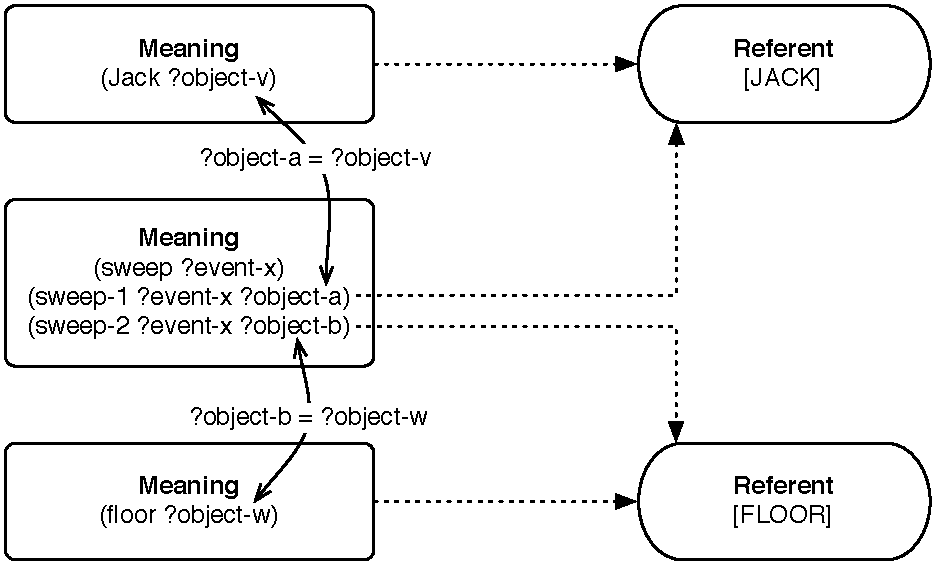
\includegraphics[width=0.8\linewidth]{Chapter2/figs/sweep-1}}
  \caption[Linking the meanings of an event]{One of the primary functions of grammar is to indicate how different meanings should be linked to each other. In the present formalization, this is represented through variable equal\is{variable equality}ities: the variables `?object-u' and `?object-a' should be made equal\is{variable equality} because they both refer to [JACK]; and the variables `?object-v' and `?object-b' should be made equal\is{variable equality} because they both refer to [FLOOR].}
   \label{f:linking}
\end{figure}

\ea
$\exists$ ?object-a, ?object-b, ?object-c, ?event-x: jack(?object-a) $\wedge$ floor(?object-b) $\wedge$ sweep(?event-x) $\wedge$ sweep-1(?event-x , ?object-a) $\wedge$ sweep-2(?event-x, ?object-b) $\wedge$ sweep-3(?event-x, ?object-c)
\item $\exists$ ?object-a, ?object-b, ?object-c, ?event-x: jack(?object-a) $\wedge$ dust(?object-b) $\wedge$ floor(?object-c) $\wedge$ sweep(?event-x) $\wedge$ sweep-1(?event-x, ?object-a) $\wedge$ sweep-2(?event-x, ?object-b) $\wedge$ sweep-3(?event-x, ?object-c)
\z

\section{A brief introduction to Fluid Construction Grammar}

\begin{figure}
\centerline{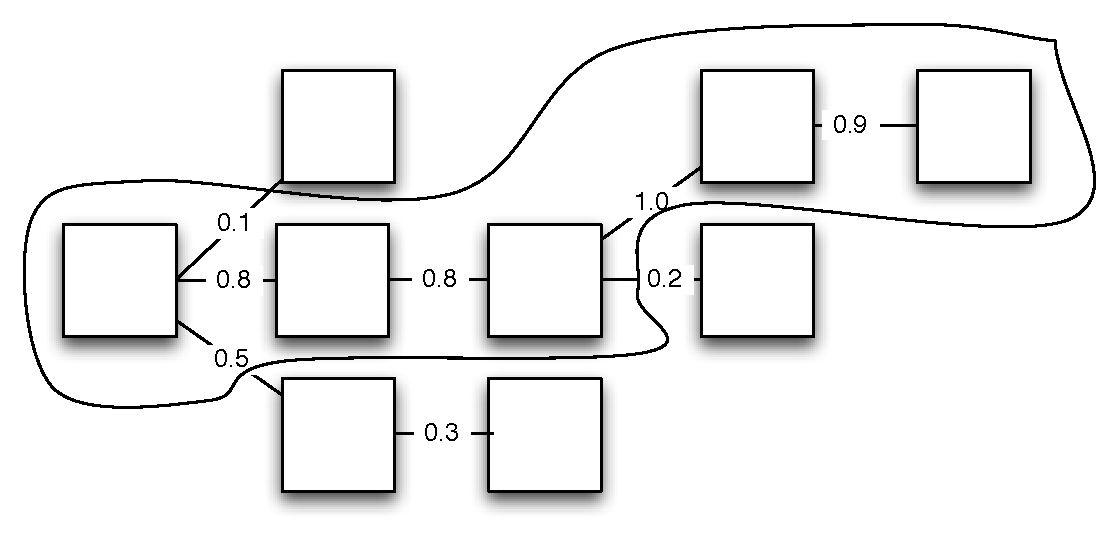
\includegraphics[width=0.8\linewidth]{Chapter2/figs/reaction-network}}
  \caption[A reaction network\is{reaction network}]{During processing, the language user builds up a reaction network\is{reaction network} by trying out constructions. The pathway with the highest confidence\is{confidence} scores is selected for producing or parsing an utterance.}
   \label{f:reaction}
\end{figure}

As already mentioned before, Fluid Construction Grammar is a computational grammar formalism for bidirectional language processing, learning and evolution. During linguistic processing, the FCG-system is either provided with a meaning that needs to be verbalized (production) or an utterance that needs to be analyzed into a meaning (parsing). The FCG-system then builds up a `reaction network\is{reaction network}' (or search tree; see Figure \ref{f:reaction}) in which each node represents a stage in the build-up of the semantic and syntactic structure of an utterance. 

Traveling from one node to the next can be achieved by applying a construction (i.e. a conventionalized mapping between meaning and form). Since there may be several hypotheses given a certain context, each link between the nodes has a `confidence\is{confidence} score' to guide the search. This score is based on (a) the (linguistic) context in which constructions can be applied, and (b) how successful the applied constructions have been in previous communicative situations. The system will in the end choose the chain with the highest estimated success.

FCG\is{construction grammar!Fluid Construction Grammar} uses many well-known techniques from computational linguistics such as term unification\is{unification} and feature structure\is{feature structure}s to represent linguistic knowledge. In fact, all linguistic knowledge (including constructions) is represented as {\bfseries coupled feature structure\is{feature structure!coupled feature structure}s}, which couple a semantic pole to a syntactic pole. All feature structure\is{feature structure}s are organized in units which are used by the basic operators of FCG\is{construction grammar!Fluid Construction Grammar} for retrieving and adding new feature-value pairs. Thus, all linguistic knowledge is represented according to the following pattern:

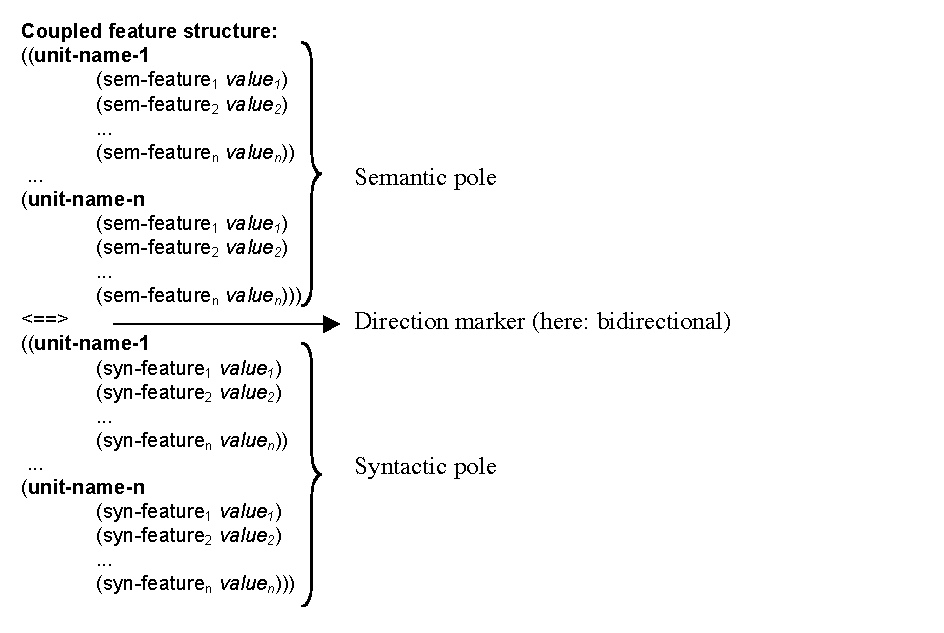
\includegraphics[width=\linewidth]{Chapter2/figs/fcg-pattern}

\begin{figure}[p]
\centerline{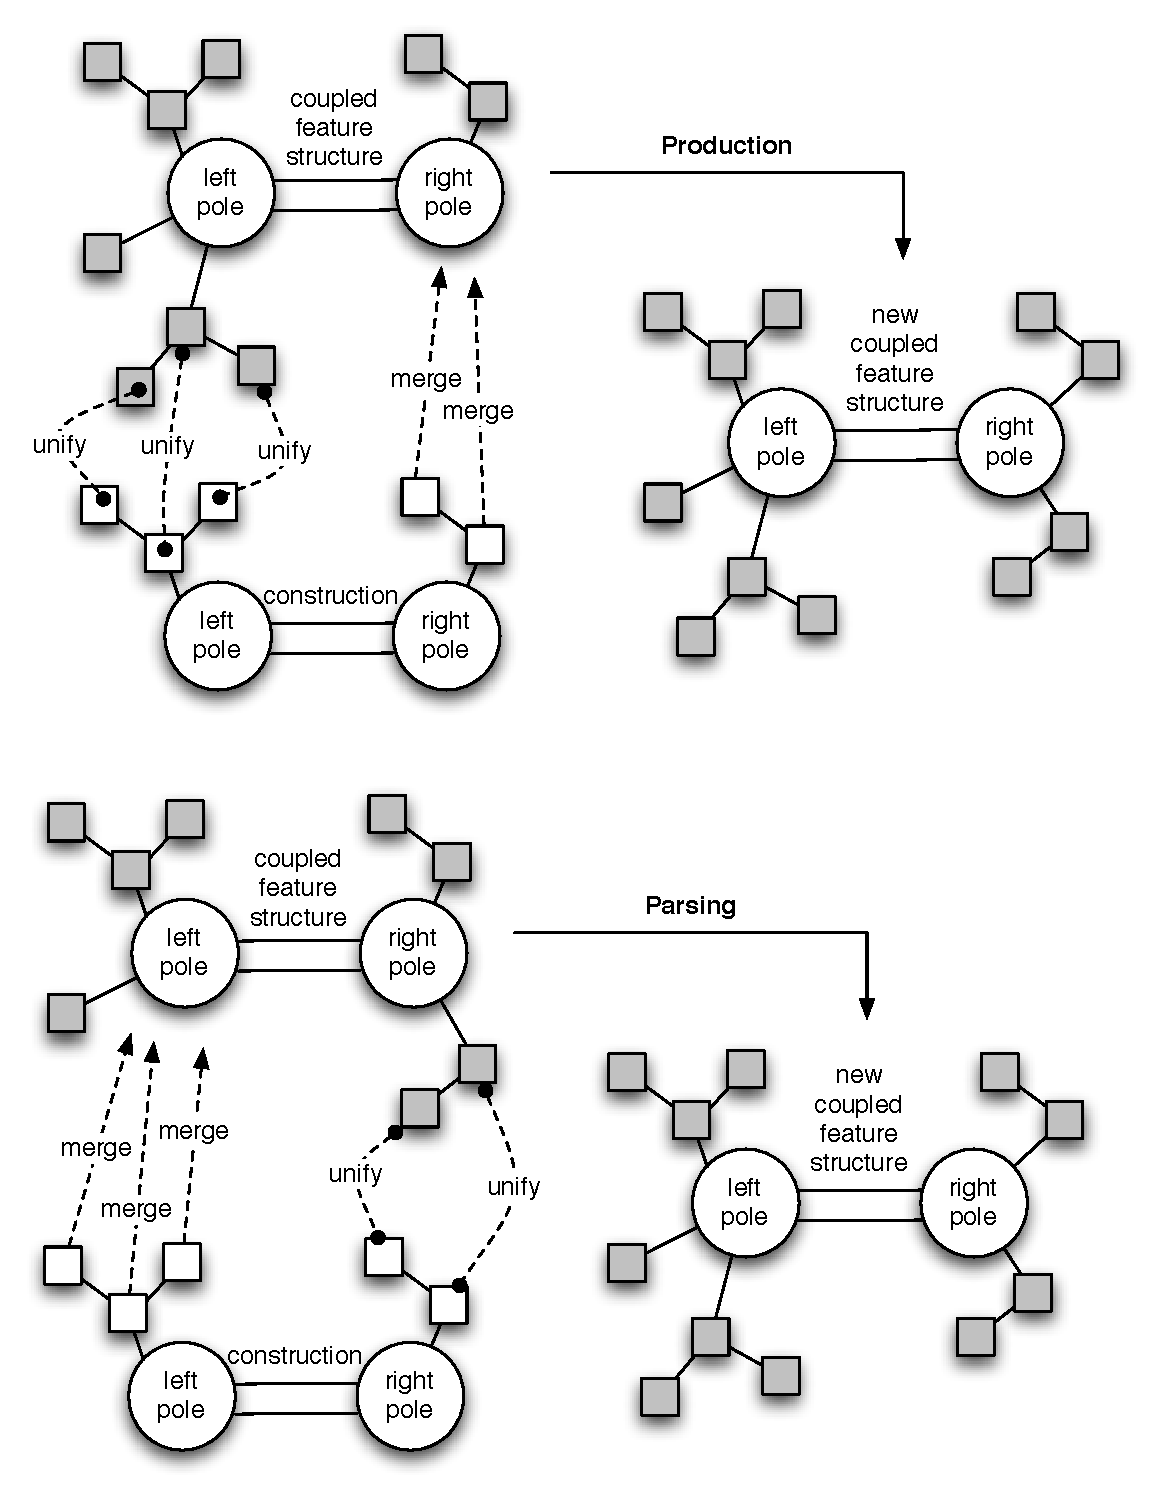
\includegraphics[width=0.8\linewidth]{Chapter2/figs/unify}}
 \caption[Unifying and merging a construction]{During production, the feature structure\is{feature structure}s (squares) in the left pole of a construction (bottom left in top figure) are unified with those of the current coupled feature structure\is{feature structure!coupled feature structure} (top left in top figure). If unification\is{unification} is successful, the right pole is merged with the coupled feature structure\is{feature structure!coupled feature structure}. This yields a new coupled feature structure\is{feature structure!coupled feature structure}, which is a new node in the reaction network\is{reaction network} (right). During parsing, the same operation is performed but this time the right pole of the construction is unified and the left one is merged with the current node.}
   \label{f:unify}
\end{figure}

\vspace{0.3cm}
\noindent{\bfseries Unify and Merge.} The two basic operations performed in FCG\is{construction grammar!Fluid Construction Grammar} are called `unify' and `merge' \citep[not to be confused with `merge' in Minimalis\is{Minimalist Program}m]{steels06unify}. These operators decide whether or not a construction can be applied in order to obtain a new node in the reaction network. `Unify' means that -- depending on the direction of processing -- the feature structure\is{feature structure} of one of the poles of a construction acts as a set of constraints that have to be compatible with the corresponding pole of the current node in the reaction network\is{reaction network}. If all the constraints are satisfied, the other pole is `merged' with the corresponding pole in the current node (unless merging fails because of conflicts in both poles). The combination of the unify\is{unify and merge} and merge operations leads to a new coupled feature structure\is{feature structure!coupled feature structure}, which is the next node in the reaction network\is{reaction network} (see Figure \ref{f:unify}).

Constructions can be applied bidirectional\is{bidirectionality}ly using the same operations, so parsing and production use the same linguistic knowledge but in opposite directions. Achieving both production and parsing is a non-trivial problem, and some formalisms therefore focus exclusively on either production or parsing (e.g. Embodied Construction Grammar). FCG\is{construction grammar!Fluid Construction Grammar} makes no claim that {\em all} linguistic knowledge is bidirectional\is{bidirectionality}, but uses bidirectional\is{bidirectionality} application of constructions for coupling input to output so that agents equipped with FCG can act both as speakers and as hearers. 

When in production mode, the FCG-system unifies the left pole of a construction (typically the semantic pole) with that of the current node; and if successful it merges the right pole (typically the syntactic pole) with that of the current node. During parsing, exactly the same linguistic items are used, but this time in the opposite direction: here, the right pole has to unify\is{unify and merge} with the corresponding pole in the current node after which the left pole can be merged with its corresponding pole in the current node.
\\
\\
\noindent{\bfseries Structure building.} FCG has a special operator -- called the `J-operator' -- for specifying hierarchical relations between units. Roughly speaking, all units marked with a J-operator\is{structure building!J-operator} are ignored during the unification\is{unification} phase, but are added or merged during the merge operation. I will limit my discussion here to the functions of the J-operator\is{structure building!J-operator} that are relevant for the constructions in this chapter. For a more technical specification, see \citet[chapter 4]{debeule07compositionality} and \citet{debeule05hierarchy}. The basic syntax of the J-operator is shown in example \ref{ex:j-operator}.

\ea
\label{ex:j-operator}
\footnotesize{\begin{verbatim}
((J ?unit ?parent (?child-1 ... ?child-n))
  (feature-1 value-1)
  ...
  (feature-n value-n))
\end{verbatim}}
\z

In this syntax, the variable `?unit' has to be bound to some unit in the coupled feature structure\is{feature structure!coupled feature structure}. If the unification\is{unification} phase did not yield a binding for this variable yet, a new unit will be built. This unit is then made a sub-unit of the unit that matches with the second argument of the J-operator\is{structure building!J-operator}. In this example this is the unit that is bound to the variable `?parent'. The J-operator\is{structure building!J-operator} can also take an optional third argument, which is a list of the units which have to be made sub-units of the unit that is bound to the first argument of the J-operator\is{structure building!J-operator} (?unit). Next, additional feature-value pairs can be listed which are merged to the structure by the J-operator\is{structure building!J-operator}. I will illustrate the J-operator\is{structure building!J-operator} through an example. Suppose that we only have the top-unit on one of the poles in the coupled feature structure\is{feature structure!coupled feature structure} and that there is a construction containing the following J-unit:

{\footnotesize\begin{verbatim}
((J ?new-unit ?top-unit))
\end{verbatim}
}

Since there is no unit yet which could have been bound to the variable ?new-unit during the unification\is{unification} phase, a new unit is created. This unit is then made a sub-unit of the unit that is bound to the second argument of the J-operator\is{structure building!J-operator} so that we get the following structure:

\ea
\Tree[.Top-unit New-unit ]
\z

Suppose now that another construction applies which contains the following J-unit:

{\footnotesize\begin{verbatim}
((J ?another-new-unit ?top-unit (?new-unit)))
\end{verbatim}}

Let's assume that the variable ?top-unit was bound by the unifier to `top-unit' and that the variable `?new-unit' was already bound to `new-unit' (which depends on the unification\is{unification} of the units that were not marked by the J-operator\is{structure building!J-operator}). The variable `?another-new-unit' does not have a binding yet so a new unit is built, which is made a sub-unit of `top-unit'. This time there is also a third argument of the J-operator\is{structure building!J-operator}. All the units in this list are made sub-units of the newly created unit so we get the following structure:

\ea
\Tree[.Top-unit [.Another-new-unit New-unit ] ]
\z

Another use of the J-operator\is{structure building!J-operator} that is adopted in this thesis is the possibility of merging additional feature-value pairs to an existing unit. This can be done as follows:

{\footnotesize\begin{verbatim}
((J ?unit NIL)
  (feature-1 value-1)
  ...
  (feature-n value-n))
\end{verbatim}}

If the second argument of the J-operator\is{structure building!J-operator} is an empty list (NIL), no structure building operation needs to be performed. In this case, the J-operator\is{structure building!J-operator} will only try to merge the feature-value pairs that are specified with the structure of the unit which is bound to the first argument of the J-operator\is{structure building!J-operator} (?unit). This functionality is needed because it allows the merging of new feature-value pairs on the same pole after successful unification\is{unification} rather than only merging the other pole of the construction to the coupled feature structure\is{feature structure!coupled feature structure}. In other words, it allows a construction to add both semantic {\em and} syntactic feature-value pairs to the coupled feature structure\is{feature structure!coupled feature structure}.

It should be noted that the above tree-like representation of hierarchical structure is only a visualization. The units of a construction or coupled feature structure are only elements of a flat list and are themselves not hierarchically organized. Instead, hierarchical relations in the linguistic structure are explicitly represented as feature-value pairs using the feature `sem-subunits' on the semantic pole and the feature `syn-subunits' on the syntactic pole.

\section{Parsing ``Jack sweep dust off-floor''}

With the meaning representation and FCG\is{construction grammar!Fluid Construction Grammar} overview in mind, we can now dive into more details of the operationalization. This section illustrates parsing using the sentence {\em Jack sweep dust off- floor} is parsed, which is a simplification of the sentence {\em Jack sweeps the dust off the floor}. Obviously, this section does not provide a description of an actual English utterance, but only highlights the problem of argument realization while ignoring issues such as agreement, determination, and so on.

At the beginning of the parsing process, the FCG-system creates a first node in a reaction network\is{reaction network}, which is a coupled feature structure\is{feature structure!coupled feature structure} with an empty semantic and syntactic pole. I assume here that the utterance is segmented into the separate strings ``jack'', ``sweep'', ``dust'', ``off-'' and ``floor''. These strings are all lumped together along with the observed word order\is{word order} (i.e. the `meets'-constraints) into the form-feature of one unit on the syntactic pole, which I will call the top-unit. The label `top-unit' is arbitrary but makes interpretation easier for human readers. On  the semantic pole, the corresponding unit (also called `top-unit') is still empty:
\\
\\
{\footnotesize{\tt <Node-1: coupled-feature-structure
\\ ((top-unit))
\\ <==>
\\ ((top-unit
\\ \hspace*{5mm} (form 
\\ \hspace*{12mm}((string jack-unit ``jack'') (string sweep-unit ``sweep'')
\\ \hspace*{13mm} (string dust-unit ``dust'') (string off-unit ``off-'')
\\ \hspace*{13mm} (string floor-unit ``floor'') (meets jack-unit sweep-unit)
\\ \hspace*{13mm} (meets sweep-unit dust-unit) (meets dust-unit off-unit)
\\ \hspace*{13mm} (meets off-unit floor-unit)))))>}}

\subsection{Unifying and merging lexical entries}
\label{s:example-parsing}

In the next step, the FCG-system performs a lexical look-up for all the words in the utterance. For this, we need a lexical entries (also called lexical constructions). The lexical entr\is{lexical entry}y for {\em jack} looks as follows: 
\\
\\
{\footnotesize{\tt <Lexical entry: jack
\\ ((?top-unit
\\ \hspace*{5mm} (meaning (== (jack ?object-1))))
\\ \hspace*{2mm}((J ?new-unit ?top-unit)
\\ \hspace*{5mm} (referent ?object-1)
\\ \hspace*{5mm} (sem-cat animate\is{animacy}-object)))
\\ <==>
\\ ((?top-unit
\\ \hspace*{5mm} (form (== (string ?new-unit ``jack''))))
\\ \hspace*{2mm}((J ?new-unit ?top-unit)
\\ \hspace*{5mm} (syn-cat (== (pos noun\is{noun})))))>}}
\\
\\
Note that the lexical entr\is{lexical entry}y for {\em jack} contains variable\is{logic variable}s not only for the meaning but also for the unit-names. The unification\is{unification} engine of FCG\is{construction grammar!Fluid Construction Grammar} can use these variable\is{logic variable}s to match them against the unit-structure of the current node in the reaction network\is{reaction network}. Since we're in parsing mode, the right pole of the entry (under the directional marker {\tt <==>}) needs to be unified with the right-pole of node-1. The right pole specifies that there has to be some unit ({\tt ?top-unit}) which must contain the feature {\tt form}, which itself must contain in its value the feature-value {\tt (string ?new-unit ``jack'')}. These constraints are indeed satisfied: the variable {\tt ?top-unit} can be bound to the unit {\tt top-unit} in the current node because it fulfills all the necessary conditions.

Since unification\is{unification} is successful, the left pole, which contains the meaning of the lexical entr\is{lexical entry}y, can be merged with the left pole of node-1. The units that are marked with the J-operator\is{structure building!J-operator} were ignored during the unification\is{unification} phase, but are now integrated: the J-operator\is{structure building!J-operator} pulls the lexical information for {\em jack} down into a new unit and specifies that this new-unit is a sub-unit of the top-unit. The J-operator\is{structure building!J-operator} also merges additional features with this new unit concerning its referent and its semantic and syntactic categorization. One could devise many other categorizations and features for {\em jack}, but they are not necessary for understanding the example here so they are left out for convenience's sake.

Since both unification\is{unification} and merge were successful, a new node is created in the reaction network\is{reaction network}. Here we see that the other words are still in the top-unit, but that there is a new unit for {\em jack} (which I conveniently label `jack-unit' here but this may be any arbitrary symbol) both in the semantic and in the syntactic pole:
\\
\\
{\footnotesize{\tt <Node-2: coupled-feature-structure
\\ ((top-unit
\\ \hspace*{5mm} (sem-subunits (jack-unit)))
\\ \hspace*{2mm}(jack-unit
\\ \hspace*{5mm} (meaning ((jack ?object-1)))
\\ \hspace*{5mm} (referent ?object-1)
\\ \hspace*{5mm} (sem-cat animate\is{animacy}-object)))
\\ <==>
\\ ((top-unit
\\ \hspace*{5mm} (syn-subunits (jack-unit))
\\ \hspace*{5mm} (form 
\\ \hspace*{10mm} ((string sweep-unit ``sweep'') (string dust-unit ``dust'') 
\\ \hspace*{11mm} (string off-unit ``off-'') (string floor-unit ``floor'') 
\\ \hspace*{11mm} (meets jack-unit sweep-unit) (meets sweep-unit dust-unit) 
\\ \hspace*{11mm} (meets dust-unit off-unit) (meets off-unit floor-unit))))
\\ \hspace*{2mm}(jack-unit
\\ \hspace*{5mm} (form ((string jack-unit ``jack'')))
\\ \hspace*{5mm} (syn-cat ((pos noun\is{noun})))))>}}
\\
\\
The lexical entr\is{lexical entry}ies for {\em dust} and {\em floor} look almost exactly the same, apart from their semantic categorization and meaning. Both entries also unify\is{unify and merge} and merge successfully with the current node and build new nodes in the reaction network\is{reaction network}: 
\\
\\
{\footnotesize{\tt <Lexical entry: dust
\\ ((?top-unit
\\ \hspace*{5mm} (meaning (== (dust ?object-2))))
\\ \hspace*{2mm}((J ?new-unit ?top-unit)
\\ \hspace*{5mm} (referent ?object-2)
\\ \hspace*{5mm} (sem-cat moveable-object)))
\\ <==>
\\ ((?top-unit
\\ \hspace*{5mm} (form (== (string ?new-unit ``dust''))))
\\ \hspace*{2mm}((J ?new-unit ?top-unit)
\\ \hspace*{5mm} (syn-cat (== (pos noun\is{noun})))))>}
\\
\vspace*{2mm}
\\
{\tt <Lexical entry: floor
\\ ((?top-unit
\\ \hspace*{5mm} (meaning (== (dust ?object-3))))
\\ \hspace*{2mm}((J ?new-unit ?top-unit)
\\ \hspace*{5mm} (referent ?object-3)
\\ \hspace*{5mm} (sem-cat surface-object)))
\\ <==>
\\ ((?top-unit
\\ \hspace*{5mm} (form (== (string ?new-unit ``floor''))))
\\ \hspace*{2mm}((J ?new-unit ?top-unit)
\\ \hspace*{5mm} (syn-cat (== (pos noun\is{noun})))))>}}\\
\\
The lexical entr\is{lexical entry}y for {\em sweep}, however, is a bit more complicated. Its main function is the same as for the other lexical entr\is{lexical entry}ies: given the string ``sweep'', it will merge the meaning of this word with the semantic pole of the current node in the reaction network\is{reaction network}. The main difference with the other words lies in the semantic and syntactic categorization of {\em sweep}. Take a look at the features `syn-frame' in the syntactic pole and `sem-frame' in the semantic pole:
\\
\\
{\tt <Lexical entry: sweep
\\ ((?top-unit
\\ \hspace*{5mm} (meaning (== (sweep ?event-x)
\\ \hspace*{32mm}(sweep-1 ?event-x ?obj-x)
\\ \hspace*{32mm}(sweep-2 ?event-x ?obj-y)
\\ \hspace*{32mm}(sweep-2 ?event-x ?obj-z))))
\\ \hspace*{2mm}((J ?new-unit ?top-unit)
\\ \hspace*{5mm} (sem-frame (== (sem-role-agent ?unit-a ?obj-x)
\\ \hspace*{36mm}(sem-role-surface ?unit-b ?obj-y)
\\ \hspace*{36mm}(sem-role-moveable ?unit-c ?obj-y)
\\ \hspace*{36mm}(sem-role-source ?unit-d ?obj-z)))))
\\ <==>
\\ ((?top-unit
\\ \hspace*{5mm} (form (== (string ?new-unit ``sweep''))))
\\ \hspace*{2mm}((J ?new-unit ?top-unit)
\\ \hspace*{5mm} (syn-cat (== (pos verb\is{verb})))
\\ \hspace*{5mm} (syn-frame (== (syn-role-subject ?unit-1)
\\ \hspace*{36mm}(syn-role-object ?unit-2)
\\ \hspace*{36mm}(syn-role-oblique ?unit-3)))))>}
\\
\\
At first glance, it seems that the lexical entr\is{lexical entry}y contains a predicate or case frame that lists the valence of a verb\is{verb} as in traditional lexicalis\is{lexicalist}t approaches. The big difference with most other approaches is however that these frames do not directly list the \is{event structure}argument structure of the verb\is{verb} but only its {\bfseries potential valent\is{valency!potential valents}s}. For example, the syn-frame only states that {\em sweep} can occur in an \is{event structure}argument structure in which there may be some unit playing the role of subject\is{syntactic role!subject}, some unit playing the role of object\is{syntactic role!object}, some unit playing the role of oblique\is{syntactic role!oblique}, or several units playing a combination of these roles. None of these roles are however obligatory: the verb\is{verb} remains agnostic as to which of these valents actually should be realized or what the possible combinations may be. I will show later that it is the construction that will select from the potential valent\is{valency!potential valents}s what the {\bfseries actual valen\is{valency!actual valency}cy} of the verb\is{verb} is or will be in the utterance (also see Figure \ref{f:sweep-quadrant}).
\begin{figure}[t]
\centerline{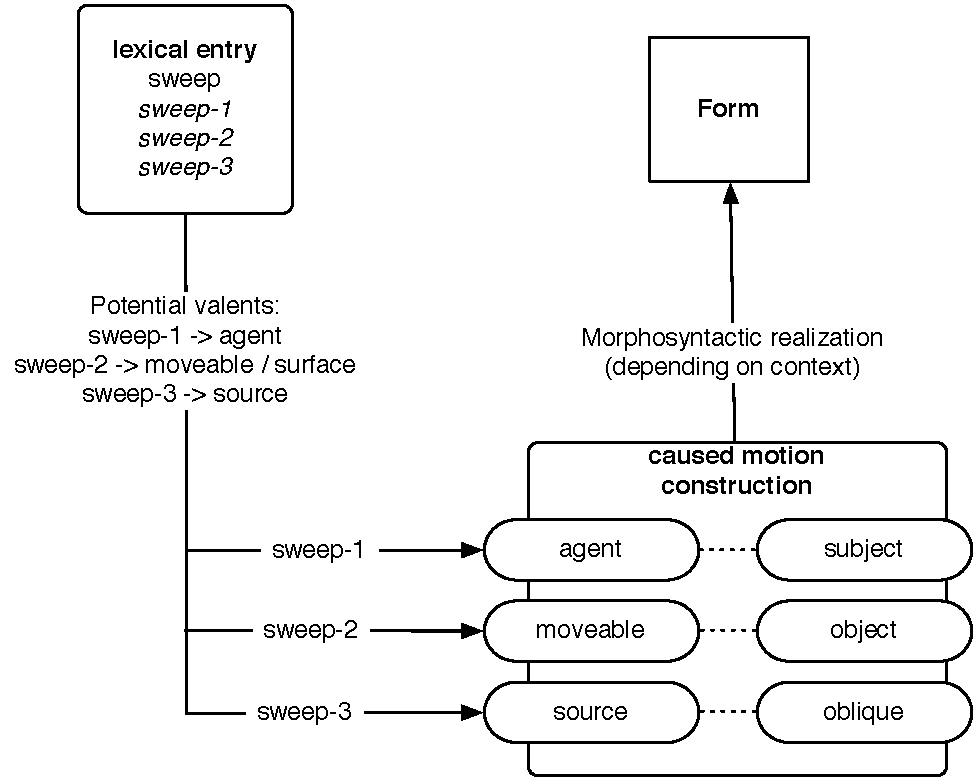
\includegraphics[width=0.8\linewidth]{Chapter2/figs/quadrant}}
 \caption[Integrating {\em sweep} with the Caused-Motion Construction]{The relation between the meaning of an event and its morphosyntactic realization is indirect and multilayered. This figure shows how a lexical entr\is{lexical entry}y introduces its `potential valent\is{valency!potential valents}s' from which the construction selects the actual valen\is{valency!actual valency}cy combination. The construction then maps this meaning onto a syntactic pattern, which in itself is realized as a certain form (depending on linguistic and extra-linguistic context)}
   \label{f:sweep-quadrant}
\end{figure}

This architecture of potential valent\is{valency!potential valents}s is mirrored in the semantic frame\is{frame!semantic frame}. Here too, the verb\is{verb} only lists all its potential valent\is{valency!potential valents}s: there may be an agent\is{semantic role!agent} role, a surface role, a moveable role, or a source\is{semantic role!source} role. The sem-frame does not specify which of these roles actually have to be realized, nor what the possible combinations are. It does specify, however, how these potential valences should be linked to the verb\is{verb}-specific participant role\is{participant role}s in the meaning feature. For example, `sem-role-agent' is linked to `sweep-1' because they share the variable `?obj-x'. `Sem-role-source' is linked to `sweep-3' because they share the variable `?obj-z'. The participant role\is{participant role} `sweep-2' is even linked to two different potential valent\is{valency!potential valents}s: `sem-role-surface' and `sem-role-moveable'. The lexical entr\is{lexical entry}y thus allows participant role\is{participant role}s to be mapped onto different semantic role\is{semantic role}s.

Both the sem- and syn-frame also contain variables that have to be bound to the unit-names of the arguments to which the roles may be assigned later on. For example, the variable `?unit-1' should be bound to the unit that plays the role of subject\is{syntactic role!subject} (if present). Notice, however, that this variable is not the same one as the variable name of the unit that may play the agent\is{semantic role!agent} role (if present): `?unit-a'. In most other grammar formalisms, such as HPSG\is{Head-Driven Phrase Structure Grammar}, a direct link between `agent\is{semantic role!agent}' and `subject\is{syntactic role!subject}' is assumed and alternating \is{event structure}argument structures such as passive\is{construction!passive construction}s are {\em deriv\is{derivation}ed} through lexical rule\is{lexical rule}s. {\bfseries I do not assume such a link between subject\is{syntactic role!subject} and agent\is{semantic role!agent}}: having two different variable names reflects the fact that both can be bound to different units as is the case in the passive\is{construction!passive construction} voice. I therefore consider the passive\is{construction!passive construction} as an alternative \is{event structure}\is{construction!argument structure construction}argument structure construction instead of a deriv\is{derivation}ational one. An active\is{construction!active construction} construction links agent\is{semantic role!agent} and subject\is{syntactic role!subject} to each other by making their variables equal\is{variable equality}, whereas the passive\is{construction!passive construction} construction features a different pattern by making other variables equal\is{variable equality} (e.g. those of the subject\is{syntactic role!subject} and the surface role as in {\em The floor was swept}). Here again, it is the construction that decides and not the verb\is{verb}. I will return to this matter in Chapter \ref{c:impact-linguistics}.

The next two Chapters will demonstrate how these potential valents can be gradually acquired and constructed through language use. They should therefore not be seen as a rigid set of possibilities or as some set of innate categories. Instead the potential uses of a verb\is{verb} can be exten\is{extension}ded (and shrunk) if needed for communicative purposes, and each possibility may become convention\is{convention}alized or become obsolete in the speech community\is{speech population}.

Unifying and merging the lexical entr\is{lexical entry}ies for {\em sweep}, {\em floor} and {\em dust} (the ordering does not matter) will lead the hearer to a fifth node in the reaction network\is{reaction network}:
\\
\\
{\footnotesize{\tt <Node-5: coupled-feature-structure
\\ ((top-unit
\\ \hspace*{5mm} (sem-subunits (jack-unit sweep-unit dust-unit floor-unit)))
\\ \hspace*{2mm}(jack-unit
\\ \hspace*{5mm} (meaning ((jack ?object-1)))
\\ \hspace*{5mm} (referent ?object-1)
\\ \hspace*{5mm} (sem-cat animate\is{animacy}-object))
\\ \hspace*{2mm}(sweep-unit
\\ \hspace*{5mm} (meaning ((sweep ?event-x)
\\ \hspace*{27mm}(sweep-1 ?event-x ?obj-x)
\\ \hspace*{27mm}(sweep-2 ?event-x ?obj-y)
\\ \hspace*{27mm}(sweep-3 ?event-x ?obj-z)))
\\ \hspace*{5mm} (sem-frame ((sem-role-agent ?unit-a ?obj-x)
\\ \hspace*{30mm}(sem-role-surface ?unit-b ?obj-y)
\\ \hspace*{30mm}(sem-role-moveable ?unit-c ?obj-y)
\\ \hspace*{30mm}(sem-role-source ?unit-d ?obj-z))))
\\ \hspace*{2mm}(dust-unit
\\ \hspace*{5mm} (meaning ((dust ?object-2)))
\\ \hspace*{5mm} (referent ?object-2)
\\ \hspace*{5mm} (sem-cat moveable-object))
\\ \hspace*{2mm}(floor-unit
\\ \hspace*{5mm} (meaning ((floor ?object-3)))
\\ \hspace*{5mm} (referent ?object-3)
\\ \hspace*{5mm} (sem-cat surface-object)))
\\ <==>
\\ ((top-unit
\\ \hspace*{5mm} (syn-subunits (jack-unit sweep-unit dust-unit floor-unit))
\\ \hspace*{5mm} (form 
\\ \hspace*{10mm}((string off-unit ``off-'') (meets jack-unit sweep-unit)
\\ \hspace*{11mm} (meets sweep-unit dust-unit) (meets dust-unit off-unit)  
\\ \hspace*{11mm} (meets off-unit floor-unit))))
\\ \hspace*{2mm}(jack-unit
\\ \hspace*{5mm} (form ((string jack-unit ``jack'')))
\\ \hspace*{5mm} (syn-cat ((pos noun\is{noun}))))
\\ \hspace*{2mm}(sweep-unit
\\ \hspace*{5mm} (form ((string sweep-unit ``sweep'')))
\\ \hspace*{5mm} (syn-cat ((pos verb\is{verb})))
\\ \hspace*{5mm} (syn-frame ((syn-role-subject ?unit-1)
\\ \hspace*{30mm}(syn-role-object ?unit-2)
\\ \hspace*{30mm}(syn-role-oblique ?unit-3))))
\\ \hspace*{2mm}(dust-unit
\\ \hspace*{5mm} (form ((string dust-unit ``dust'')))
\\ \hspace*{5mm} (syn-cat ((pos noun\is{noun}))))
\\ \hspace*{2mm}(floor-unit
\\ \hspace*{5mm} (form ((string floor-unit ``floor'')))
\\ \hspace*{5mm} (syn-cat ((pos noun\is{noun})))))>}}
\\
\\
The meanings in the above coupled feature structure\is{feature structure!coupled feature structure} are however still unlinked (see section \ref{s:linking}). In other words, the hearer knows at this stage the meaning of the individual words, but not who is doing what in the sweep-event: the variables that accompany the meaning of {\em sweep} (`?obj-x', `?obj-y' and `?obj-z') are not shared by any of the arguments (`?object-1', `?object-2' and `?object-3'). We therefore need to unify\is{unify and merge} and merge the correct construction that is able to handle the unresolved variable equalities.

\subsection{A syntactic case marker\is{case!case marking}}
\label{s:morph-rule}

Before that construction is applied, there is still the string ``off-'' in the top-unit that needs to be parsed. In this example I analyze {\em off-} as some kind of simple case marker\is{case!case marking} that assigns the oblique\is{syntactic role!oblique} case to the argument that immediately follows it. By treating {\em off-} as a case marker\is{case!case marking} I can immediately illustrate how marker\is{case!case marking}s are represented in the experiments as well.

In line with its definition in section \ref{s:stage4}, a syntactic case marker\is{case!case marking} is dissociat\is{dissociation}ed from a particular semantic role\is{semantic role}. I therefore implement case marker\is{case!case marking}s in a morphological rule or construction (a `morph-rule') in which both the left and the right pole are syntactic (so both poles operate on the syntactic pole of the current node in the reaction network\is{reaction network}). One could say in this approach that a case marker\is{case!case marking} has a syntactic or grammatical meaning rather than a semantic one. The notion of potential valent\is{valency!potential valents}s can also be applied to capture the polysemous nature of case marker\is{case!case marking}s, but for simplicity's sake I will assume here that there is a one-to-one mapping between the syntactic role\is{syntactic role} `oblique' and the marker\is{case!case marking} {\em off-}.

The morph-rule specifies that, during parsing, there needs to be a unit which contains in its form-feature the string ``off-'' and a word order\is{word order} constraint that says that the marker\is{case!case marking} immediately precedes (`meets') some other unit. If this unifies (and it does with the right pole of node-5), the left pole merges with the syntactic pole of the current node in the reaction network\is{reaction network}. The information added here is that the role of oblique\is{syntactic role!oblique} is assigned to the other unit (which immediately followed the marker\is{case!case marking}). Note that this other unit should already be present in the current node as a sub-unit of the top-unit. This is indeed the case: the variable `?some-unit' can be bound to `floor-unit' which was already present after unify\is{unify and merge}ing and merging the lexical entr\is{lexical entry}y of {\em floor}.

The morph-rule also contains a two-legged operation using the J-operator\is{structure building!J-operator}: in a first step, a new unit is created for {\em off-}, and in a second step the J-operator\is{structure building!J-operator} specifies that the newly-made unit must become a sub-unit of the other unit that immediately followed it (floor-unit). Without repeating the entire coupled feature structure\is{feature structure!coupled feature structure}, the syntactic structure now looks as follows:
\\
\\
\centerline{\Tree [ .top-unit jack-unit sweep-unit dust-unit [ .floor-unit off-unit ] ]}
\\
\\
The morphological rule itself looks as follows:
\\
\\
{\footnotesize{\tt <Morph-rule: off-
\\ ((?top-unit
\\ \hspace*{5mm} (syn-subunits (== ?some-unit)))
\\ \hspace*{2mm}(?some-unit
\\ \hspace*{5mm} (syn-role syn-role-oblique)))
\\ <==>
\\ ((?top-unit
\\ \hspace*{5mm} (form (== (string ?marker-unit ``off-'')
\\ \hspace*{24mm} (meets ?marker-unit ?some-unit))))
\\ \hspace*{2mm}((J ?marker-unit ?top-unit))
\\ \hspace*{2mm}((J ?some-unit ?top-unit (?marker-unit))))>}}


\subsection{The cause\is{causality}d motion construction\is{construction!caused motion construction}}

The utterance {\em Jack sweeps the dust off the floor} is a typical example of the cause\is{causality}d motion construction\is{construction!caused motion construction} \citep[chapter 7]{goldberg95construction}, which here carries the meaning of `X cause\is{causality}s Y to move Z by sweeping'. In the semantic pole, the construction selects from the verb\is{verb} the semantic role\is{semantic role}s of agent\is{semantic role!agent}, moveable patient\is{semantic role!patient} and source\is{semantic role!source}. On the syntactic pole it assigns the syntactic role\is{syntactic role}s of subject\is{syntactic role!subject}, object\is{syntactic role!object} and oblique\is{syntactic role!oblique} to the arguments. The construction looks as follows:
\\
\\
{\footnotesize{\tt <Construction: caused-motion
\\ ((?top-unit
\\ \hspace*{5mm} (sem-subunits (== ?unit-a ?unit-b ?unit-c ?unit-d)))
\\ \hspace*{2mm}(?unit-a
\\ \hspace*{5mm} (sem-frame (== (sem-role-agent ?unit-b ?obj-x)
\\ \hspace*{36mm}(sem-role-moveable ?unit-c ?obj-y)
\\ \hspace*{36mm}(sem-role-source ?unit-d ?obj-z))))
\\ \hspace*{2mm}(?unit-b
\\ \hspace*{5mm} (referent ?obj-x)
\\ \hspace*{5mm} (sem-cat animate\is{animacy}-object))
\\ \hspace*{2mm}(?unit-c
\\ \hspace*{5mm} (referent ?obj-y)
\\ \hspace*{5mm} (sem-cat moveable-object))
\\ \hspace*{2mm}(?unit-d
\\ \hspace*{5mm} (referent ?obj-z)))
\\ <==>
\\ ((?top-unit
\\ \hspace*{5mm} (syn-subunits (== ?unit-a ?unit-b ?unit-c ?unit-d))
\\ \hspace*{5mm} (form ((meets ?unit-b ?unit-a) (meets ?unit-a ?unit-c)
\\ \hspace*{19mm} (meets ?unit-c ?unit-d))))
\\ \hspace*{2mm}(?unit-a
\\ \hspace*{5mm} (syn-cat (== (pos verb\is{verb})))
\\ \hspace*{5mm} (syn-frame (== (syn-role-subject ?unit-b)
\\ \hspace*{36mm}(syn-role-object ?unit-c)
\\ \hspace*{36mm}(syn-role-oblique ?unit-d))))
\\ \hspace*{2mm}(?unit-d
\\ \hspace*{5mm} (syn-role syn-role-oblique))
\\ \hspace*{2mm}((J ?unit-b NIL)
\\ \hspace*{5mm} (syn-role syn-role-subject))
\\ \hspace*{2mm}((J ?unit-c NIL) 
\\ \hspace*{5mm} (syn-role syn-role-object)))>}}
\\
\\
Since the hearer is parsing, the right pole needs to be unified with the current node in the reaction network\is{reaction network}. The right pole here demands there to be some unit with at least four sub-units and with a certain word order\is{word order} among them (i.e. the `meets'-constraints). The last argument also has to have the syntactic role\is{syntactic role} of oblique\is{syntactic role!oblique}. The right pole of the current node satisfies all the constraints: jack-unit receives subject\is{syntactic role!subject} status and dust-unit becomes the object. The unit for {\em floor} was already marked as oblique\is{syntactic role!oblique} by the morphological rule that was shown in the previous section.

Thanks to the word-order constraints, the construction can unambiguously bind the variables `?unit-b' to `jack-unit', `?unit-c' to `dust-unit' and `?unit-d' to `floor-unit'. The construction then links the syntactic role\is{syntactic role}s to the semantic role\is{semantic role}s by making the necessary variables equal\is{variable equality}: the subject\is{syntactic role!subject} jack-unit is assigned the role of agent\is{semantic role!agent}, the object\is{syntactic role!object} dust-unit is assigned the role of moveable (object) and the oblique\is{syntactic role!oblique} floor-unit is assigned the role of source\is{semantic role!source}. By doing so, the construction can also link the meanings to each other: sem-role-agent shares the variable `?obj-x' with sweep-1 and the referent of jack-unit, sem-role-moveable shares the variable `?obj-y' with sweep-2 and the referent of dust-unit, and sem-role-source shares the variable `?obj-z' with sweep-3 and the referent of floor-unit. This leads to the following node in the reaction network\is{reaction network}:
\\
\\
{\footnotesize{\tt <Node-7: coupled-feature-structure
\\ ((top-unit
\\ \hspace*{5mm} (sem-subunits (jack-unit sweep-unit dust-unit floor-unit)))
\\ \hspace*{2mm}(jack-unit
\\ \hspace*{5mm} (meaning ((jack ?obj-x)))
\\ \hspace*{5mm} (referent ?obj-x)
\\ \hspace*{5mm} (sem-role sem-role-agent)
\\ \hspace*{5mm} (sem-cat animate\is{animacy}-object))
\\ \hspace*{2mm}(sweep-unit
\\ \hspace*{5mm} (meaning ((sweep ?event-x)
\\ \hspace*{27mm}(sweep-1 ?event-x ?obj-x)
\\ \hspace*{27mm}(sweep-2 ?event-x ?obj-y)
\\ \hspace*{27mm}(sweep-3 ?event-x ?obj-z)))
\\ \hspace*{5mm} (sem-frame ((sem-role-agent jack-unit ?obj-x)
\\ \hspace*{30mm}(sem-role-surface dust-unit ?obj-y)
\\ \hspace*{30mm}(sem-role-moveable dust-unit ?obj-y)
\\ \hspace*{30mm}(sem-role-source floor-unit ?obj-z))))
\\ \hspace*{2mm}(dust-unit
\\ \hspace*{5mm} (meaning ((dust ?obj-y)))
\\ \hspace*{5mm} (referent ?obj-y)
\\ \hspace*{5mm} (sem-role sem-role-moveable)
\\ \hspace*{5mm} (sem-cat moveable-object))
\\ \hspace*{2mm}(floor-unit
\\ \hspace*{5mm} (meaning ((floor ?obj-z)))
\\ \hspace*{5mm} (referent ?obj-z)
\\ \hspace*{5mm} (sem-role sem-role-source)
\\ \hspace*{5mm} (sem-cat surface-object)))
\\ <==>
\\ ((top-unit
\\ \hspace*{5mm} (syn-subunits (jack-unit sweep-unit dust-unit floor-unit))
\\ \hspace*{5mm} (form ((meets jack-unit sweep-unit) 
\\ \hspace*{19mm} (meets sweep-unit dust-unit)
\\ \hspace*{19mm} (meets dust-unit off-unit)))) 
\\ \hspace*{2mm}(jack-unit
\\ \hspace*{5mm} (form ((string jack-unit ''jack'')))
\\ \hspace*{5mm} (syn-role syn-role-subject)
\\ \hspace*{5mm} (syn-cat ((pos noun\is{noun}))))
\\ \hspace*{2mm}(sweep-unit
\\ \hspace*{5mm} (form ((string sweep-unit ''sweep'')))
\\ \hspace*{5mm} (syn-cat ((pos verb\is{verb})))
\\ \hspace*{5mm} (syn-frame ((syn-role-subject jack-unit)
\\ \hspace*{30mm}(syn-role-object dust-unit)
\\ \hspace*{30mm}(syn-role-oblique foor-unit))))
\\ \hspace*{2mm}(dust-unit
\\ \hspace*{5mm} (form ((string dust-unit ''dust'')))
\\ \hspace*{5mm} (syn-role syn-role-object)
\\ \hspace*{5mm} (syn-cat ((pos noun\is{noun}))))
\\ \hspace*{2mm}(floor-unit
\\ \hspace*{5mm} (syn-subunits (off-unit))
\\ \hspace*{5mm} (form ((string floor-unit ''floor'')))
\\ \hspace*{5mm} (syn-role syn-role-oblique)
\\ \hspace*{5mm} (syn-cat ((pos noun\is{noun}))))
\\ \hspace*{2mm}(off-unit
\\ \hspace*{5mm} (form ((string off-unit ''off-'') 
\\ \hspace*{19mm} (meets off-unit floor-unit)))))>}}
\\
\\
Now we can extract the following meaning from the semantic pole of the coupled feature structure:

\ea
$\exists$ ?obj-x, ?obj-y, ?obj-z, ?event-x: jack(?obj-x) $\wedge$ dust(?obj-y) $\wedge$ floor(?obj-z) $\wedge$ sweep(?event-x) $\wedge$ sweep-1(?event-x , ?obj-x) $\wedge$ sweep-2(?event-x, ?obj-y) $\wedge$ sweep-3(?event-x, ?obj-z)
\z

As can be seen in the meaning, all variables that refer to the same referent have been made equal\is{variable equality} by the construction. The hearer thus knows that {\em jack} was the sweeper, that {\em dust} was the thing being swept, and that the {\em floor} was the source\is{semantic role!source} of the motion. In the experiments reported in this book, the agents will then match this parsed meaning against their world model.

\section{Producing ``jack sweep floor''}

This section gives an overview of how an utterance such as {\em jack sweep floor} can be produced in Fluid Construction Grammar\is{construction grammar!Fluid Construction Grammar}. In this case, the cause\is{causality}d motion construction\is{construction!caused motion construction} is not used, but a construction which maps the semantic frame\is{frame!semantic frame} `X acts on surface Y' onto the syntactic frame\is{frame!syntactic frame} `Subject-Verb\is{verb}-Object'. The speaker starts with the following meaning (in which NIL stands for `empty' or `not profiled\is{event profile}'):

\ea
((jack object-1) (floor object-2) (sweep event-1) 
\\ \hspace*{3mm}(sweep-1 event-1 object-1) (sweep-2 event-1 object-2) 
\\ \hspace*{3mm}(sweep-3 event-1 NIL))
\z

In order to verb\is{verb}alize this meaning, the speaker constructs a reaction network\is{reaction network}. The first node in the network is a coupled feature structure\is{feature structure!coupled feature structure} in which the entire meaning is placed into one unit in the semantic pole, and in which the syntactic pole is still empty:
\\
\\
{\footnotesize{\tt <Node-1: coupled-feature-structure
\\ ((top-unit
\\ \hspace*{5mm} (meaning ((jack object-1) (floor object-2)
\\ \hspace*{24mm} (sweep event-1) (sweep-1 event-1 object-1)
\\ \hspace*{24mm} (sweep-2 event-1 object-2) (sweep-3 event-1 NIL)))))
\\ <==>
\\ ((top-unit))>}}

\subsection{Unifying and merging lexical entr\is{lexical entry}ies}

Next, the speaker builds new nodes in the network by unify\is{unify and merge}ing and merging the lexical entr\is{lexical entry}ies that cover these meanings. Suppose that the speaker has the same lexical entr\is{lexical entry}ies as given in the previous section and that all three of them ({\em jack, sweep} and {\em floor)} are a successful match, then the new coupled feature structure\is{feature structure!coupled feature structure} looks as follows:
\\
\\
{\footnotesize{\tt <Node-4: coupled-feature-structure
\\ ((top-unit
\\ \hspace*{5mm} (sem-subunits (jack-unit sweep-unit floor-unit)))
\\ \hspace*{2mm}(jack-unit
\\ \hspace*{5mm} (meaning ((jack object-1)))
\\ \hspace*{5mm} (referent object-1)
\\ \hspace*{5mm} (sem-cat animate\is{animacy}-object))
\\ \hspace*{2mm}(sweep-unit
\\ \hspace*{5mm} (meaning ((sweep event-1)
\\ \hspace*{27mm}(sweep-1 event-1 object-1)
\\ \hspace*{27mm}(sweep-2 event-1 object-2)
\\ \hspace*{27mm}(sweep-3 event-1 NIL)))
\\ \hspace*{5mm} (sem-frame ((sem-role-agent ?unit-a object-1)
\\ \hspace*{30mm}(sem-role-surface ?unit-b object-2)
\\ \hspace*{30mm}(sem-role-moveable ?unit-c object-2)
\\ \hspace*{30mm}(sem-role-source ?unit-d NIL))))
\\ \hspace*{2mm}(floor-unit
\\ \hspace*{5mm} (meaning ((floor object-2)))
\\ \hspace*{5mm} (referent object-2)
\\ \hspace*{5mm} (sem-cat surface-object)))
\\ <==>
\\ ((top-unit
\\ \hspace*{5mm} (syn-subunits (jack-unit sweep-unit floor-unit)))
\\ \hspace*{2mm}(jack-unit
\\ \hspace*{5mm} (form ((string jack-unit ''jack'')))
\\ \hspace*{5mm} (syn-cat ((pos noun\is{noun}))))
\\ \hspace*{2mm}(sweep-unit
\\ \hspace*{5mm} (form ((string sweep-unit ''sweep'')))
\\ \hspace*{5mm} (syn-cat ((pos verb\is{verb})))
\\ \hspace*{5mm} (syn-frame ((syn-role-subject ?unit-1)
\\ \hspace*{30mm}(syn-role-object ?unit-2)
\\ \hspace*{30mm}(syn-role-oblique ?unit-3))))
\\ \hspace*{2mm}(floor-unit
\\ \hspace*{5mm} (form ((string floor-unit ''floor'')))
\\ \hspace*{5mm} (syn-cat ((pos noun\is{noun})))))>}}
\\
\\
Since the speaker knows which meaning he wants to express, there are no unresolved variable equal\is{variable equality}ities in the meanings in the semantic pole. However, so far no semantic or syntactic role\is{syntactic role}s have been assigned yet: the lexical entr\is{lexical entry}y of {\em sweep} has merely introduced its potential valent\is{valency!potential valents}s, but not its actual valen\is{valency!actual valency}cy. This is reflected by the fact that the arguments do not have the feature `sem-role' or `syn-role' yet and that there are still variables left for the unit-names in both the syn- and sem-frame. It is also still undecided which participant should be mapped onto subject\is{syntactic role!subject} and which onto object or oblique\is{syntactic role!oblique}.

\subsection{The agent-acts-on-surface construction}

Trying to unify\is{unify and merge} the cause\is{causality}d motion construction\is{construction!caused motion construction} leads to a failure: first of all, {\em floor} is categorized as a static surface-object and thus violates the construction's constraint that the patient\is{semantic role!patient} has to be moveable, and second, the source\is{semantic role!source} argument is missing. So a different construction needs to be unified and merged to travel to the next node in the network. The following `agent-acts-on-surface' construction would do the trick:

\noindent{\footnotesize{\tt <Construction: agent-acts-on-surface
\\ ((?top-unit
\\ \hspace*{5mm} (sem-subunits (== ?unit-a ?unit-b ?unit-c)))
\\ \hspace*{2mm}(?unit-a
\\ \hspace*{5mm} (sem-frame (== (sem-role-agent ?unit-b ?obj-x)
\\ \hspace*{36mm}(sem-role-surface ?unit-c ?obj-y))))
\\ \hspace*{2mm}(?unit-b
\\ \hspace*{5mm} (referent ?obj-x)
\\ \hspace*{5mm} (sem-cat animate\is{animacy}-object))
\\ \hspace*{2mm}(?unit-c
\\ \hspace*{5mm} (referent ?obj-y)
\\ \hspace*{5mm} (sem-cat surface-object)))
\\ <==>
\\ ((?top-unit
\\ \hspace*{5mm} (syn-subunits (== ?unit-a ?unit-b ?unit-c ?unit-d))
\\ \hspace*{5mm} (form ((meets ?unit-b ?unit-a) (meets ?unit-a ?unit-c))))
\\ \hspace*{2mm}(?unit-a
\\ \hspace*{5mm} (syn-cat (== (pos verb\is{verb})))
\\ \hspace*{5mm} (syn-frame (== (syn-role-subject ?unit-b)
\\ \hspace*{36mm}(syn-role-object ?unit-c))))
\\ \hspace*{2mm}((J ?unit-b NIL)
\\ \hspace*{5mm} (syn-role syn-role-subject))
\\ \hspace*{2mm}((J ?unit-c NIL) 
\\ \hspace*{5mm} (syn-role syn-role-object)))>}}
\\
\\
First the speaker tries to unify\is{unify and merge} the semantic pole with that of the current node in the reaction network\is{reaction network}. This is a success because all the constraints are satisfied: the construction expects some unit with three sub-units, one of which is an animate\is{animacy}-object and one of which is a surface-object. The construction also selects the semantic role\is{semantic role}s of `agent\is{semantic role!agent}' and `surface' from the verb\is{verb}'s potential valent\is{valency!potential valents}s and assigns them to the correct arguments. Next, the right pole of the construction is merged with the right pole of the current node. Since it is specified that the agent\is{semantic role!agent} maps onto subject\is{syntactic role!subject} and the surface maps onto object\is{syntactic role!object} in this construction, the correct syntactic role\is{syntactic role}s are assigned to the arguments, including their word order\is{word order}. The new node looks as follows:
\\
\\
{\footnotesize{\tt <Node-5: coupled-feature-structure
\\ ((top-unit
\\ \hspace*{5mm} (sem-subunits (jack-unit sweep-unit floor-unit)))
\\ \hspace*{2mm}(jack-unit
\\ \hspace*{5mm} (meaning ((jack object-1)))
\\ \hspace*{5mm} (referent object-1)
\\ \hspace*{5mm} (sem-role sem-role-agent)
\\ \hspace*{5mm} (sem-cat animate\is{animacy}-object))
\\ \hspace*{2mm}(sweep-unit
\\ \hspace*{5mm} (meaning ((sweep event-1)
\\ \hspace*{27mm}(sweep-1 event-1 object-1)
\\ \hspace*{27mm}(sweep-2 event-1 object-2)
\\ \hspace*{27mm}(sweep-3 event-1 NIL)))
\\ \hspace*{5mm} (sem-frame ((sem-role-agent jack-unit object-1)
\\ \hspace*{30mm}(sem-role-surface floor-unit object-2)
\\ \hspace*{30mm}(sem-role-moveable floor-unit object-2)
\\ \hspace*{30mm}(sem-role-source ?unit-d NIL))))
\\ \hspace*{2mm}(floor-unit
\\ \hspace*{5mm} (meaning ((floor object-2)))
\\ \hspace*{5mm} (referent object-2)
\\ \hspace*{5mm} (sem-role sem-role-surface)
\\ \hspace*{5mm} (sem-cat surface-object)))
\\ <==>
\\ ((top-unit
\\ \hspace*{5mm} (syn-subunits (jack-unit sweep-unit floor-unit))
\\ \hspace*{5mm} (form ((meets jack-unit sweep-unit) 
\\ \hspace*{18,5mm} (meets sweep-unit floor-unit))))
\\ \hspace*{2mm}(jack-unit
\\ \hspace*{5mm} (form ((string jack-unit ''jack'')))
\\ \hspace*{5mm} (syn-role syn-role-subject)
\\ \hspace*{5mm} (syn-cat ((pos noun\is{noun}))))
\\ \hspace*{2mm}(sweep-unit
\\ \hspace*{5mm} (form ((string sweep-unit ''sweep'')))
\\ \hspace*{5mm} (syn-cat ((pos verb\is{verb})))
\\ \hspace*{5mm} (syn-frame ((syn-role-subject jack-unit)
\\ \hspace*{30mm}(syn-role-object floor-unit)
\\ \hspace*{30mm}(syn-role-oblique ?unit-3))))
\\ \hspace*{2mm}(floor-unit
\\ \hspace*{5mm} (form ((string floor-unit ''floor'')))
\\ \hspace*{5mm} (syn-role syn-role-object)
\\ \hspace*{5mm} (syn-cat ((pos noun\is{noun})))))>}}
\\
\\
The speaker has no other constructions or linguistic items that could unify\is{unify and merge} and merge, so he is almost done processing. In the final phase, he takes all the formal constraints specified in the syntactic pole of the last node and renders them into the utterance {\em jack sweep floor}.

\section{Networks and conventionalization}

The previous two sections showed how lexical and constructional meanings can integrate through the potential valent\is{valency!potential valents}s of the verb\is{verb} on the one hand, and the selection\is{selection} of the actual valen\is{valency!actual valency}cy by the constructions on the other. I also suggested that the list of potential valent\is{valency!potential valents}s can be exten\is{extension}ded if needed for communication. However, this solution is too powerful because it does not explain why speakers of English\is{English} prefer not to use {\em sweep} in for example the ditransitive\is{ditransitive clause} construction as in {\em *he swept him the dust}. We therefore need an additional strategy to restrict the powers of the proposed representation.

Utterances such as {\em *he swept him the dust} are perfectly intelligible but somehow speakers (usually) refrain from using words in constructions that they are not convention\is{convention}ally associated with. Convention or entrench\is{entrenchment}ment can intuitively be captured in a network as illustrated in Figure \ref{f:network-sweep}. The basic idea is the following: we never observe words in total isolation but always in language use. We can therefore keep links between constructions that reflect their past co-occur\is{co-occurrence}rences. For example, {\em sweep} has a link to the intransitive construction, the cause\is{causality}d motion construction\is{construction!caused motion construction}, etc. The link reflects convention\is{convention}alization through a confidence\is{confidence} score: the higher this score, the more confident the speaker feels integrating the lexical entr\is{lexical entry}y with the construction. The lower the score, the more `strain' there is to go ahead and fuse the lexical entr\is{lexical entry}y with the construction. Scores in the network can be changed each time the lexical entr\is{lexical entry}y and the construction co-occur\is{co-occurrence}: the score increases if they are used in successful communication, but decreases if co-occur\is{co-occurrence}rence leads to communicative failure. Each interaction also yields the possibility of adding new links. I will come back to the exact nature of this network in the following chapters.
\begin{figure}[tb]
\centerline{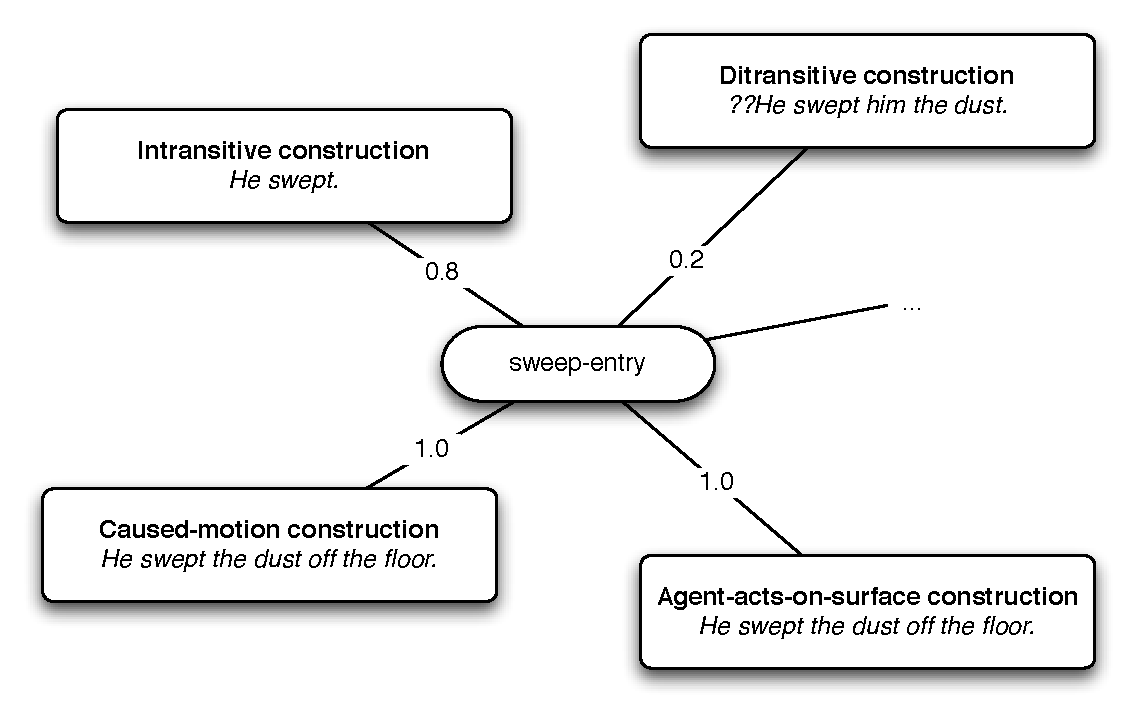
\includegraphics[width=\linewidth]{Chapter2/figs/network}}
 \caption[Network for {\em sweep}]{Lexical entries keep a link to all the constructions that they integrated with. Each link has a specific confidence\is{confidence} score which reflects how confident the language user is that the lexical entr\is{lexical entry}y can be fused with the construction. The higher the score, the more conventionalized the link is. The lower the score, the more `strain' the speaker will have to use the entry and the construction together. This network thus captures convention\is{convention}alised patterns in a language.}
   \label{f:network-sweep}
\end{figure}

% ####################################################################

\setcounter{chapter}{2}
\chapter{Baseline Experiments}
\label{c:base}

The grammatical square\is{grammatical square} (see Figure \ref{f:stage4}) illustrates the multifunctional and indirect nature of case marking\is{case!case marking}. It can also be read as a `research roadmap' for experiments on the emergence\is{formation} of a grammar for case. More specifically, the experiments must investigate how a population\is{speech population} of agents can evolve a grammar which takes care of (1) the mapping between event-specific participant role\is{participant role}s and generalized semantic role\is{semantic role}s, (2) the mapping between semantic role\is{semantic role}s and grammatical cases, and (3) the mapping between cases and surface case marker\is{case!case marking}s. Constructing and aligning this kind of grammar in a multi-agent population\is{speech population} is incredibly difficult because all mappings are agent-internal and are thus not directly observable by other agents. Moreover, these mappings vary depending on the communicative and linguistic context so the agents have to be capable of dealing with polysemy\is{polysemy}. Finally, linguistic convention\is{convention}s may constantly change so the agents have to be able to adapt to newly propagat\is{propagation}ed constructions.

In this Chapter I will present three baseline experiments which first replicate simulations reported by \citet{steels02simulating, steels04constructivist} and then lift them towards a multi-agent simulation. I will specifically focus on which diagnostic\is{learning strategies!diagnostics}s, repair\is{learning strategies!repair strategies}s and alignment strateg\is{alignment strategy}ies are needed for each step of increased complexity. In the next section, I will first give an overview of the experimental set-up that is shared by all experiments after which the simulations themselves are reported.

\section{Experimental set-up}

\begin{table}[t]
\centerline{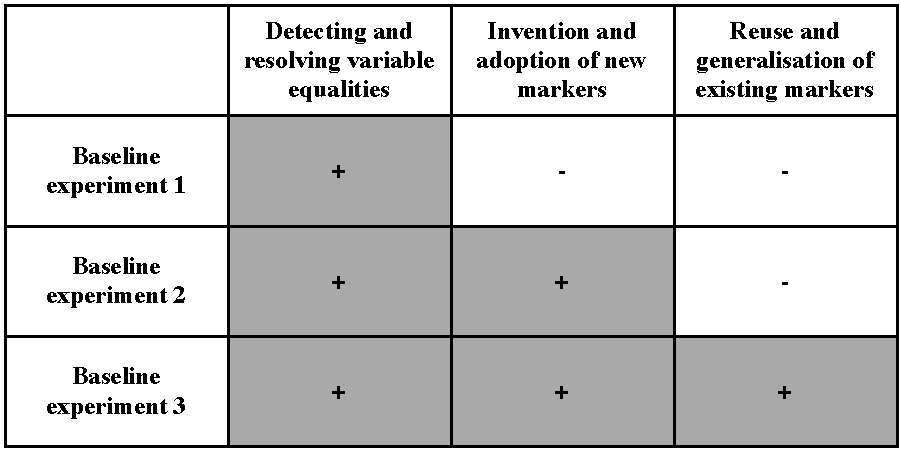
\includegraphics[width=\linewidth]{Chapter3/figs/repairs}}
\caption[Key cognitive abilities in the baseline experiments]{This table shows the key cognitive abilities which are given to the agents in the baseline experiments. In the first experiment, agents are `intelligent' enough to resolve variable equal\is{variable equality}ities by using their world model but they cannot express these equal\is{variable equality}ities in their language. In experiment 2, the agents can decide to invent new marker\is{case!case marking}s to indicate the linking of equal\is{variable equality} variables but they cannot generalize or abstract. In the third experiment, the agents can perform analog\is{analogy}ical reasoning over event structure\is{event structure}s to generalize existing marker\is{case!case marking}s.}
\label{t:repairs}
\end{table}

The simulations in this book investigate how a population\is{speech population} of artificial agents can autonomously construct a shared grammatical system for marking event structure\is{event structure} (in the form of a case grammar\is{case!case grammar}). As argued in section \ref{s:methodology}, we need to hypothesize which cognitive mechanisms and external pressures are the minimal ingredients that enable the agents to do so, and we need to operationalize them into computational processes and a world environment. Since case marking\is{case!case marking} is a complex phenomenon, I will divide the topic into several subparts that follow the stages of development identified in section \ref{s:case-markers}.

\subsection{Key abilities and self-assessment criteria}

In the problem-solving\is{problem-solving} approach adopted in this book, innovat\is{innovation}ion and language change\is{language change} happens in three steps: (1) the speaker innovat\is{innovation}es and is therefore the main cause of potential language change\is{language change}, (2) the hearer tries to infer and learn the innovat\is{innovation}ion through an `abductive process' (as opposed to uniquely relying on inducti\is{induction}on or genetically evolved innate knowledge), and (3) the innovat\is{innovation}ion propagat\is{propagation}es in the population\is{speech population}. Step (1) may be skipped when the hearer overgeneralizes or imposes more systematicity\is{systematicity} on the utterance than introduced by the speaker. Hearer-based innovat\is{innovation}ion or `reanalysis\is{reanalysis}' can be described in terms of the same cognitive processes as involved in speaker-based innovat\is{innovation}ion so the two sources of innovat\is{innovation}ion are complementary to each other \citep{hoefler08reanalysis}. Step (3) implies that an innovat\is{innovation}ion only becomes a linguistic convention\is{convention} if it has been adopted by a sufficient number of language users. Propagation is made possible through the alignment strateg\is{alignment strategy}ies of the agents.

This approach requires a population\is{speech population} of agents endowed with rich cognitive capabilities. As argued in section \ref{s:methodology}, agents can only make use of local measure\is{measure!local measure}s such as communicative success\is{communicative success} and cognitive effort\is{cognitive effort} for steering their linguistic behaviour. The cognitive mechanisms of the agents therefore have to enable the agents to move into a meta-level in which they can {\bfseries self-assess\is{self-assessment}} what problems they encounter during communication, whether there is opportunity for optimization, or what the reasons for success and failure are in a language game\is{language game}. They need to be able to couple this {\bfseries diagnosis} to {\bfseries repair\is{learning strategies!repair strategies} strategies} in order to solve their communicative problems and to their {\bfseries alignment strateg\is{alignment strategy}ies} in order to converge on a shared language. All the experiments in this book mainly focus on the effect of these three aspects: diagnostic\is{learning strategies!diagnostics}s, repair\is{learning strategies!repair strategies}s, and alignment strateg\is{alignment strategy}ies.

The baseline experiments reported in this Chapter first of all replicate the two-agent simulations reported by \citet{steels02simulating, steels04constructivist}. These experiments only focus on the first three stages of case marker\is{case!case marking} development ranging from no marking to the formation\is{formation} and marking of semantic role\is{semantic role}s. Additionally, the experiments are pushed forward to multi-agent simulations in which language convergence becomes the main issue. All three baseline experiments share the same world environment, communicative task, and assumption\is{assumption}s and scaffold\is{scaffold}s (see below). However, they differ in the {\bfseries key cognitive abilities} that the agents are endowed with. I define `key cognitive abilities' as those mechanisms that are hypothesized to be crucial for the transition in the grammar from one stage to the next, and of which the simulations need to demonstrate or falsify whether this is indeed the case. Table \ref{t:repairs} illustrates the difference between the baseline experiments in terms of key cognitive abilities and can be summarized as follows:

\begin{enumerate}
\item In baseline experiment 1 (corresponding to stage 1 -- section \ref{s:stage1}), agents are given the diagnostic\is{learning strategies!diagnostics} to figure out how the meanings of lexical items are linked to each other by exploiting the situatedness\is{situatedness} of the interaction. However, the agents have no means of exten\is{extension}ding their language to explicitly mark the relations between words;
\item In baseline experiment 2 (corresponding to stage 2 -- section \ref{s:stage2}), agents are endowed with a repair\is{learning strategies!repair strategies} strategy which enables them to invent a participant role\is{participant role}-specific case marker\is{case!case marking} for optimizing communication;
\item In baseline experiment 3 (corresponding to stage 3 -- section \ref{s:stage3}), agents are endowed with the capacity to perform analog\is{analogy}ical reasoning over event structure\is{event structure}s. They can exploit this capacity for generalizing existing marker\is{case!case marking}s to cover new participant role\is{participant role}s. As I will show later, generalization is not a goal in itself but rather a side-effect of the need for optimizing communication.
\end{enumerate}

These key cognitive abilities will be explained in more detailed along with the experiments further down in this Chapter. The abilities are each time given and fixed by the experimenter and the simulations do not explain where they come from. However, the global vision underlying this work is that speakers and hearers can autonomously configure their language capacity by recruiting cognitive mechanisms that are also used for other tasks such as hierarchy\is{hierarchy} building operators \citep{steels07recruitment}. This process is driven by needs in communicative success\is{communicative success}, expressive power and the convention\is{convention}s adopted by other agents in the population\is{speech population}. Here again, agents have to be capable of self-assess\is{self-assessment}ing when to recruit a mechanism, which ones are the best candidates, and to self-regulate the semantic complexity of their communication. For simulations that investigate self-regulation and reconfiguration of the language faculty\is{language faculty} on the longer run, see \citet{steels06how-grammar, steels07scaffolding}. In the remainder of this section, I will describe those aspects of the simulations which are shared by all the experiments.

\subsection{Description games}

\begin{figure}[t]
\centerline{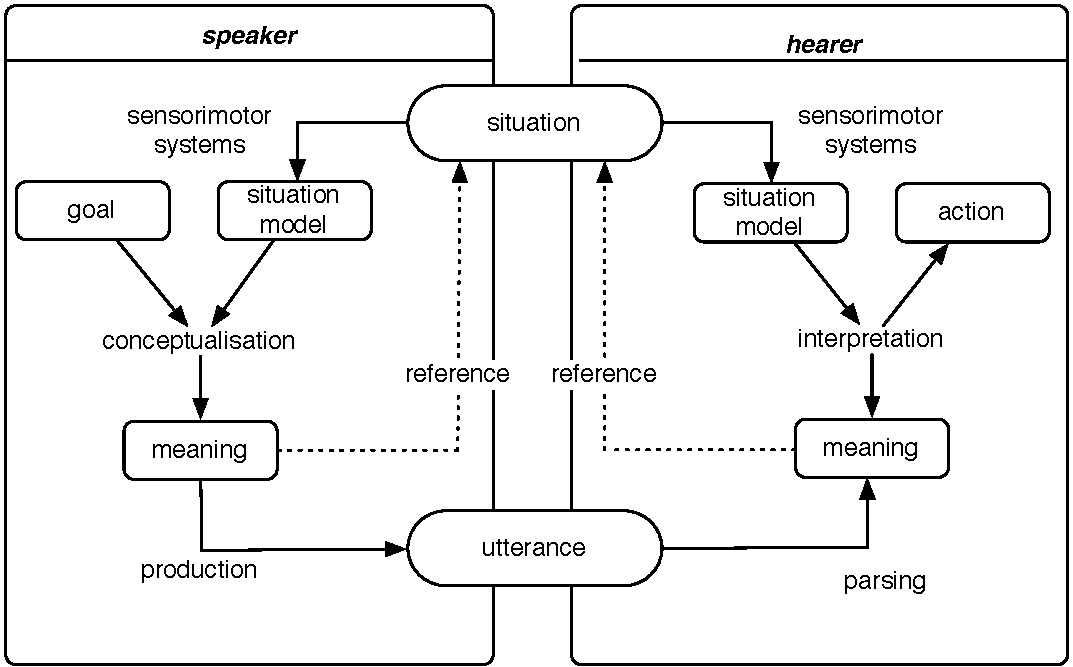
\includegraphics[width=0.8\linewidth]{Chapter3/figs/cycle}}
  \caption[The semiotic cycle]{The semiotic cycle\is{semiotic cycle} involved in language game\is{language game}s. There are three systems working in tight interaction with each other: the sensory-motor system\is{sensory-motor system} (perception and modeling), the conceptual/intentional system\is{conceptual/intentional system} (conceptualization\is{conceptualization} and interpretation), and the linguistic system (production and parsing). This book mainly focuses on the latter one and is complementary to other research efforts on grounded language use and conceptualization\is{conceptualization}.}
   \label{f:cycle}
\end{figure}

An obvious requirement for developing a grammar for marking event structure\is{event structure} is {\bfseries communication about events}. This is operationalized in the form of the {\bfseries description game\is{language game!description game}}, a routinized communicative interaction which involves the complete semiotic cycle\is{semiotic cycle} as illustrated in Figure \ref{f:cycle}. Applied to the simulations in this book, the interaction pattern conforms to the following script:

\begin{enumerate}
\item Two agents are randomly selected from the population\is{speech population}. One will act as speaker, the other as hearer. The speaker and hearer start a {\bfseries local language game\is{language game}} so the other agents cannot observe it;
\item {\bfseries Joint attention\is{joint attention}} \citep{tomasello95jointattention} between the agents is required and assumed. This is operationalized by giving the agents a shared context. The context contains one or more events (depending on the complexity of the game) which are observed by the agents;
\item Both the speaker and the hearer build a {\bfseries world model} based on the observed events. The world model consists of a series of facts in the memory;
\item The speaker is given a communicative goal. In this book, the goal is always to {\bfseries make an assertion} about a certain state of affairs in the context (i.e. the speaker has to describe an event);
\item The speaker chooses an event to describe and {\bfseries conceptualizes} a meaning for it. Conceptualization involves profiling\is{event profile} of the event and finding a discriminating meaning for the participants in the event (see further below);
\item The speaker then verb\is{verb}alizes the meaning by {\bfseries producing} an utterance which is transmitted to the hearer;
\item The hearer observes the utterance and {\bfseries parses} it;
\item The hearer then {\bfseries interprets} the parsed meaning by comparing it to the facts in the world model. This leads to the {\bfseries mental action} of agreeing or disagreeing with the description;
\item The hearer signals agreement with the description if the parsed meaning is unambiguously compatible with the hearer's world model, or signals disagreement if it is not. Agreement means {\bfseries communicative success\is{communicative success}}, disagreement means {\bfseries communicative failure}. No other kinds of feedback or requests for information are included;
\item Based on the outcome of the game, both agents {\bfseries consolidate} their linguistic inventor\is{linguistic inventory}ies. 
\end{enumerate}

\subsection{The world, sensory-motor input and conceptualization}
\label{s:world}

\begin{figure}[t]
\centerline{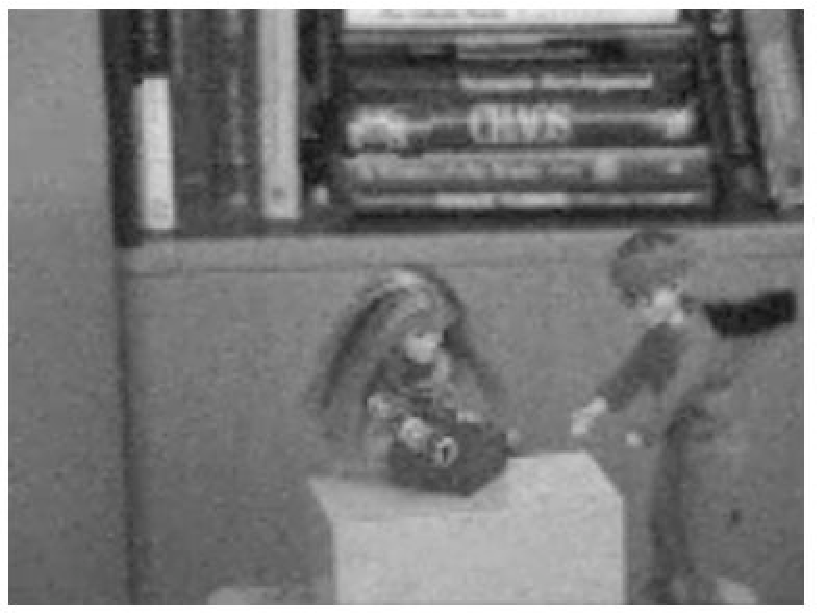
\includegraphics[width=0.65\linewidth]{Chapter3/figs/puppets}}
  \caption[An example scene]{The world environment consists of dynamic scenes in which puppets perform various actions such as walking and pushing blocks to each other. Here, one puppet `gives' a block to another puppet by sliding it over a table. The scene contains four participants (two puppets, a block and a table), a `ground' and various micro- and macro-events.}
   \label{f:puppets}
\end{figure}

The semiotic cycle\is{semiotic cycle} in Figure \ref{f:cycle} clearly shows that linguistic processing is only one part of the general cognitive architecture which is involved in communication. Even though the experiments in this book mainly focus on the production and parsing of linguistic utterances, at least two other systems are directly relevant for communication: the sensory-motor system\is{sensory-motor system} (in a broad sense responsible for dealing with the sensory experience and for building a world model) and the conceptual-intentional system (responsible for conceptualization\is{conceptualization} and interpretation as well as concept\is{concept formation} formation\is{formation}). These three `systems' work together in tight interaction and without a clear-cut division between them.

In this section, I will describe what kind of world environment is used in the experiments, what kind of world model is built by the sensory-motor system\is{sensory-motor system}, and what kind of meanings are conceptualized for communication. These three elements remain constant and are shared by all the experiments.


\subsubsection{The environment}
 The environment in the experiments consists of dynamic real-world scenes from a small puppet theater. The puppets perform various actions such as moving, disappearing from a scene, walking towards each other, and carrying objects. The use of real-world scenes is part of earlier work on grounded language communication \citep{steels02simulating, steels03shared} and is not essential to the dynamics of the models reported in this book: a simulated world suffices for the scope of this book and can in fact be used for scaling up the experiments to larger worlds. The choice for using data from real-world scenes was made in order to demonstrate that the models {\em can} be incorporated into research on the grounding of communication.

For the baseline experiments, 20 different scenes were recorded comprising 207 event token\is{event token}s belonging to 15 different event types. There are 103 event token\is{event token}s which take one participant (e.g. a `move-event'), 99 event token\is{event token}s which potentially take two participants (e.g. a `walk-to'-event) and 5 event token\is{event token}s which potentially involve three participants (e.g. a `give-event'). Given the conceptualization\is{conceptualization} algorithm (see below), this leads to a frequency\is{frequency} of about 64\% of utterances involving one participant, about 34\% of utterances involving two participants and only 2\% of utterances involving three participants. In most experiments each event type\is{event type} was given the same frequency\is{frequency} in order to balance this skewed frequency\is{frequency}. As I will demonstrate later, equal\is{variable equality} frequency\is{frequency} offers a much clearer picture of the propagat\is{propagation}ion and convergence dynamics in the experiments.


\subsubsection{Sensory-motor input}
 The real-world scenes were recorded using two SONY pan-tilt cameras (EVI-D31) which were hooked up to computers running the PERACT\is{PERACT system} system \citep{baillie00action, steels03shared}, which was designed for the visual recognition of events and which is related to other attempts in visual-recognition such as \citet{siskind00visual}. Even though two cameras were used, this book uses only the data obtained through one of them. The simulations are thus not affected by differences in world models due to noisy recognition of the events or differences in visual perspective. These difficulties are very interesting for investigating the robustness of the model in grounded communication, but are not part of this book.

Since the vision system is quite complex (but fortunately well-documented in \citealp{baillie00action}), I will restrict my discussion to its general architecture and to the design choices that are important for understanding what information is delivered to the language system. The PERACT\is{PERACT system} system first delineates objects based on colour\is{colour} histograms and then groups the pixels belonging to the same object together. These objects (two puppets, a table, two blocks, etc.) were learned in advance and PERACT\is{PERACT system} can handle seven of them simultaneously in one scene. Starting from basic visual `primitives' or `micro-events' such as touching, movement and appearance, the system tracks the objects in real-time and assembles more complex descriptions (or `macro-events') when it recognizes a pattern in the scene. This recognition is often unreliable, but saliency\is{saliency}, confidence\is{confidence} and hierarchy\is{hierarchy} are used to categorize the scene in terms of micro- and macro-events. This categorization of events is then supplied to the linguistic system.

For each agent, the filtered results of sensory processing is then represented as a series of facts in the memory. For example, an event in which one of the puppets `moves inside a yellow house' is represented as follows:

\ea
\label{facts}
\begin{lstlisting}
(move-inside event-163190 true)
(move-inside-1 event-163190 jill)
(move-inside-2 event-163190 house-1)
(girl jill) (jill jill) (house house-1) 
(yellow house-1) (boy jack) (jack jack)
\end{lstlisting}
\z

As can be seen in example \ref{facts}, there are three objects in the scene (two puppets called `Jack' and `Jill', and a house), but only two of them are participants in the move-inside-event (`Jill' and the house). For each object, the vision system delivers at least two facts which can be used during conceptualization\is{conceptualization} for discriminating the objects from the other ones in the same scene (see below). These facts are very simple (for example `house' and `yellow' for the house-object), but can be interpreted in a more general sense as being the features describing an object (e.g. in a more detailed implementation, the feature-values of a R(ed)G(reen)B(lue)-channel\is{RGB-channel} could be used instead of the feature `yellow').

The labels of these facts thus carry English\is{English} names, {\bfseries but should not be interpreted as such}. For example, `move-inside' actually involves a puppet moving behind another object. The vision system, which is based on colour\is{colour} recognition, does not have any notion of a container or some kind of `insideness'. Instead it sees one colour\is{colour} blob (the girl puppet) moving towards another one (the yellow `house') until the colour\is{colour} regions `touch' each other after which the girl puppet disappears out of sight. So the label `move-inside' does not reflect what actually happens in the scene (in terms of human conceptualization\is{conceptualization}) but it is used for facilitating the analysis of the event recognition\is{event recognition} by the experimenter.

From the above it should also be clear that the PERACT\is{PERACT system} system describes dynamic scenes in different levels of complexity. For example, the move-inside-event is itself a macro-event which can be decomposed into sub-events (which are macro-events themselves or micro-events, and which are also represented as facts in the memories of the agents). The micro-events for a move-inside-event are primitive relations such as `visible', `distance-decreasing', `movement', `touching' and `disappearing'. The PERACT\is{PERACT system} system offers a hierarchical description of events including time stamps for their beginnings and ends. As I will explain in section \ref{s:base3}, the simulations reported in this book disregard this temporal and hierarchical information and treat the event structure\is{event structure} of an event as a flat list of micro-events. This choice was made in order to focus on the participant role\is{participant role}s as a whole rather than on causal-\is{causality}aspect\is{aspect}ual parts of the event-structure. I will come back to this choice when discussing the experiments on Stage IV in the development of case markers.

One final remark regarding the sensory-motor input has to do with the status of the visual `primitives'. I do not make any claims about whether they are innate or not, nor do I claim that they represent a realistic set for categorizing events in human cognition (neither in terms of size nor in terms of quality). The idea is rather that events can be decomposed into a much richer representation that allows analog\is{analogy}ical reasoning and the comparison of event structure\is{event structure}s.


\subsubsection{Conceptualization}
 The categorization of the scenes in terms of event type\is{event type}s and objects (and their features) is already taken care of by the sensory-motor system\is{sensory-motor system}. Conceptualization in the simulations is therefore a very basic, but nonetheless crucial operation. First of all, during conceptualization\is{conceptualization} the speaker agent decides on the {\bfseries event profile} that it wants to express. `Event profile' should be interpreted in roughly the same way as commonly assumed in cognitive linguistics \citep[see for instance][]{croft98event}. Since the agents do not take temporal-aspect\is{aspect}ual information of the events into account, profiling\is{event profile} events essentially consists of deciding which participants have to be expressed explicitly. For the aforementioned move-inside-event, the speaker can thus conceptualize three different event profiles so the agents have to be able to deal with multiple argument realization\is{argument realization}:

\begin{itemize}
\item One in which only the puppet `Jill' is expressed (playing the participant role\is{participant role} `move-inside-1');
\item One in which only the object `house' is expressed (playing the participant role\is{participant role} `move-inside-2');
\item One in which both participants are expressed.
\end{itemize}

The meaning of events is a simple copy of the facts in the memory of the agent, so the meaning of the move-inside-event would simply be conceptualized as:

\ea
\label{facts2}
\begin{lstlisting}
 
(move-inside event-163190 true)
(move-inside-1 event-163190 jill)
(move-inside-2 event-163190 house-1)
\end{lstlisting}
\z

For those objects that have to be expressed explicitly according to the event profile, the agent plays a simple discrimination game\is{discrimination game} \citep{steels96perceptually, steels97constructing}. Suppose that the agents observe a scene in which there are two blocks represented as the following facts:

\ea
\begin{lstlisting}
 
(ball object-1) (blue object-1)
(ball object-2) (green object-2)
\end{lstlisting}
\z

If the agent wants to talk about the blue ball, it needs a feature or a feature set which discriminates this ball from the green one. Since both objects have the feature `ball', this cannot be used for discriminating the blue ball from the green one. The colour\is{colour}-feature, however, is discriminating so the speaker would conceptualize the following meaning for the blue ball:

\ea
\begin{lstlisting}
(blue object-1)
\end{lstlisting}
\z

If there are more than one discriminating features (e.g. the features `girl' and `jill' in example \ref{facts} both discriminate the puppet `Jill' from the puppet `Jack'), the agent randomly chooses one. The objects are defined in such a way that there is always at least one feature discriminating them from other objects in the same scene.

Suppose that the speaker profiles the move-inside-event such that only the house-object has to be expressed explicitly -- roughly meaning something like `(something) moved inside the house / the yellow thing'. Conceptualization could then possibly yield the following meanings:

\ea
\label{facts3}
\begin{lstlisting} 
(move-inside event-163190 true)
 (move-inside-1 event-163190 jill)
 (move-inside-2 event-163190 house-1)
 (yellow house-1)
\end{lstlisting}
\z

\subsection{Additional assumption\is{assumption}s and scaffold\is{scaffold}s}
\label{s:assumptions}

The agents in these simulations are endowed with strong (cognitive) capacities that enable them to communicate linguistically with each other. Listing all aspects of language that are assumed, scaffold\is{scaffold}ed or ignored would take too much space, so I will restrict myself to the most important ones:

\begin{itemize}
\item The agents are assumed to be social and cooperative. All agents are equally involved in the formation\is{formation} of their language, so the simulations ignore the possible influence of differences in social status;
\item All agents are `adult' language users. No growth of cognitive capabilities occurs and the models do not take specific child language acquisition\is{child language acquisition}\is{acquisition} restrictions into account. All agents are endowed with the same capacities;
\item The agents are assumed to be able to communicate about compositional meanings (i.e. meanings which are related to each other in some way). In the simulations, Fluid Construction Grammar\is{construction grammar!Fluid Construction Grammar} is used as a formalization of the capacity to combine and manipulate hierarchical symbolic form-meaning mappings. The models further ignore how these symbolic units should be coupled to neurological processing;
\item The agents do not have real `speech'. Instead, all utterances are perfectly transmitted from the speaker to the hearer in the form of strings of words. The influence of phonological changes on grammaticalization processes is well understood in theoretical linguistics, but computational models on the formation\is{formation} of phonological and syllabic convention\is{convention}s are scarce and not advanced enough to be used for example to model phonological reduction\is{phonological reduction} \citep[although see][]{steels98stochasticity}. The phonological development of case marker\is{case!case marking}s is therefore ignored in this book, but remains a topic of interest for the future;
\item The agents also do not care about morphology. There is no meaningful word-internal structure and the capacity of segmentation is assumed. The language-specific segmentation process is scaffold\is{scaffold}ed so the agents can perfectly cut up utterances into words and marker\is{case!case marking}s. The marker\is{case!case marking}s themselves can thus be seen as adposition\is{adposition}s rather than as true marker\is{case!case marking}s found in case languages such as German\is{German}.
\end{itemize}

Another very important scaffold\is{scaffold} is the fact that the agents start with a {\bfseries predefined lexicon\is{lexicon}, but no grammar}. There are several reasons for giving the agents a lexicon\is{lexicon} in advance. One reason is methodological: as in any other kind of controlled experiment, this book focuses only on the emergence of a case grammar\is{case!case grammar} and not on the formation\is{formation} of a lexicon\is{lexicon}. Other experiments have already extensively investigated how adaptive lexicon\is{lexicon}s can be formed and shared by large population\is{speech population}s of agents (see section \ref{s:history-lex}). All forces working on the lexicon\is{lexicon} are therefore completely scaffold\is{scaffold}ed. This also means that the meanings of lexical entr\is{lexical entry}ies are fixed and known by the agents, so they never have to perform word sense disambiguation\is{word sense disambiguation} either. One of the future steps of the research program would, however, involve the integration of lexical and grammatical development in order to verify whether the current results and conclusions remain valid.

A second reason has to do with a very important assumption that the mechanisms underlying the {\em very first} emergence\is{formation} of grammatical constructions are the same ones as those identified in attested cases of present-day grammaticalization\is{grammaticalization} processes. These cases (almost) always display a development from more lexical to more grammatical functions:

\begin{quote}
Grammaticalization is the gradual drift in all parts of the grammar toward tighter structures, towards less freedom in the use of linguistic expressions at all levels. Specifically, lexical items develop into grammatical items in particular constructions [...]. In addition, constructions become subject to stronger constraints and come to show greater cohesion. \\ \citet[318]{haspelmath98does}
\end{quote}

So the agents start from a lexicon\is{lexicon} and build their grammar on top of that. This strategy is however not uncontroversial in the field artificial language evolution\is{artificial language evolution}. For example, \citet{wray98protolanguage, wray02transition} argues that modern language evolved through the analysis of a holistic protolanguage. Similarly, many simulations (especially in Iterated Learning Model\is{Iterated Learning Model (ILM)}s) feature the analysis of holistic\is{holistic versus compositional languages} utterances into smaller linguistic units. Apart from the many arguments against the realism of the `holistic\is{holistic versus compositional languages} utterances-first' hypothesis (see \citealp{depauw02grael}: 345--348; and \citealp{wellens08flexible}), the most compelling argument for starting from a lexical language is Ockham's razor\is{Ockham's razor}: since there are no data available from the first language(s), we should first of all investigate what can be explained and learned from applying present and attested processes of grammaticalization\is{grammaticalization} rather than starting from a hypothetical holistic\is{holistic versus compositional languages} language \citep{hoefler08reanalysis}.

One important observation is that even though the agents start with a lexical language, case marker\is{case!case marking}s can be constructed in grammatical languages as well (see section \ref{s:case-markers}). Rather than thinking of the initial stage as a `lexical language' it is more fruitful to think of individual constructions that do not mark event structure\is{event structure} grammatically as the seedbed for grammatical marker\is{case!case marking}s. The existence of such constructions also shows that {\bfseries grammaticalization\is{grammaticalization} is not a determined process}: speakers of a language can but do not have to decide to tighten their linguistic items towards more grammatical uses.

The lexical entr\is{lexical entry}ies provide the agents with a language which conforms to what \citet[124]{gil08how} calls an `Isolated-Monocategorial-Associational Language' (IMA\is{IMA language}):

\begin{enumerate}
\item All the words are morphologically isolating (i.e. they have no internal morphological structure);
\item There are no formal grounds to distinguish syntactic categories such as noun\is{noun}s or verb\is{verb}s. The words are thus syntactically monocategorial. There is only a semantic distinction between words that refer to objects and those that predicate and refer to event type\is{event type}s;
\item Utterances are semantically associational: no grammar exists for marking event structure\is{event structure} so the hearer has to find out himself how meanings relate to each other.
\end{enumerate}

The lexical entr\is{lexical entry}ies thus look very much as those presented in section \ref{s:example-parsing} but this time no semantic or syntactic categories are assumed. The entry for words that refer to event type\is{event type}s only contain their event-specific participant role\is{participant role}s in their meaning but no potential semantic role\is{semantic role}s (yet). For example, the semantic pole of the entry of {\em give} lists a giver, a given and a givee (which have been assigned the more neutral and arbitrary labels give-1, give-2 and give-3). The form-feature in the syntactic pole simply looks for the string ``give'' and does not give any information yet about the word's potential valent\is{valency!potential valents}s. Both poles feature a J-operator\is{structure building!J-operator} which is used for pulling the form and meaning of {\em give} into a separate unit. The complete entry of {\em give} looks as follows:
 
\ea
\begin{lstlisting} 
<Lexical entry: give
 ((?top-unit
   (meaning (== (give ?event-x true)
                (give-1 ?event-x ?obj-x)
                (give-2 ?event-x ?obj-y)
                (give-2 ?event-x ?obj-z))))
  ((J ?new-unit ?top-unit)
   (referent ?event-x)))
<==>
 ((?top-unit
   (form (== (string ?new-unit "give"))))
  ((J ?new-unit ?top-unit)))>
\end{lstlisting}
\z

 
The entry of the word {\em jack} looks as follows:
\ea 
\begin{lstlisting}
<Lexical entry: jack
 ((?top-unit
   (meaning (== (jack ?object-1))))
  ((J ?new-unit ?top-unit)
   (referent ?object-1)))
<==>
 ((?top-unit
   (form (== (string ?new-unit "jack"))))
  ((J ?new-unit ?top-unit)))>
\end{lstlisting}
\z

In the baseline experiments 20 different scenes were recorded featuring 15 distinct event type\is{event type}s including ten macro-events (move-inside, move-outside, hide, give, take, cause-move-on, touch, grasp, fall and walk-to) and five micro-events (borderscreen, visible, move, distance-decreasing and approach). Every micro-event type\is{event type} (except for `borderscreen') can take the value of true or false, which leads to word-pairs such as {\em visible} versus {\em invisible}. This makes up for 19 different words that can be used for referring to events. The total number of event-specific participant role\is{participant role}s is 30 resulting from three one-place predicates (borderscreen, visible and move), nine two-place predicates (move-inside, move-outside, hide, touch, grasp, fall, walk-to, distance-decreasing and approach) and three three-place predicates (give, take and cause-move-on). The event type\is{event type}s and the corresponding words are summarized in Table \ref{t:events}.

Besides the words for event type\is{event type}s, the agents are given 11 unambiguous words for referring to objects. These words map in a one-to-one relationship to facts about objects in the memories of the agents. The words are: {\em blue, block, boy, girl, green, ground, house, jack, jill, table} and {\em yellow}. These words can be used for referring to the seven objects that occur in the twenty recorded scenes (a puppet called `Jill', a puppet called `Jack', a blue block, a green block, a table, a yellow house and the ground).

\begin{table}[htp]
\centering
\begin{tabular}{ c  c  c  c }
\lsptoprule
{\bfseries Event-types} & {\bfseries Participant role\is{participant role}s} & {\bfseries Truth} & {\bfseries Words}\\
& & {\bfseries values} & \\
\midrule
borderscreen & object-1& false & ``disappear''\\
  
\multirow{2}{*}{move } & \multirow{2}{*}{ move-1}& true & ``move''
\\
 & & false & ``rest''
\\
  
\multirow{2}{*}{visible } & \multirow{2}{*}{ visible-1}& true & ``visible''
\\
  & & false & ``invisible''
\\
  
\multirow{2}{*}{approach } &  approach-1 & true & ``approach''
\\
  & approach-2 & false & ``no-approach''
\\
  
\multirow{2}{*}{distance-decreasing }  &  distance-decreasing-1  & true & ``get-closer''
\\
   & distance-decreasing-2 & false & ``separate''
\\
  
\multirow{2}{*}{fall } &   fall-1  & \multirow{2}{*}{true} & \multirow{2}{*}{``fall''}
\\
 & fall-2 & &
\\
  
\multirow{2}{*}{grasp } &  grasp-1 & \multirow{2}{*}{true} & \multirow{2}{*}{``grasp''}
\\
 & grasp-2 & &
\\
  
\multirow{2}{*}{hide } &  hide-1  & \multirow{2}{*}{true} & \multirow{2}{*}{``hide''}
\\
 & hide-2 & &
\\
  
\multirow{2}{*}{move-inside } &  move-inside-1 & \multirow{2}{*}{true} & \multirow{2}{*}{``move-inside''}
\\
 & move-inside-2 & &
\\
  
\multirow{2}{*}{move-outside } &  move-outside-1 & \multirow{2}{*}{true} & \multirow{2}{*}{``move-outside''}
\\
  &  move-outside-2 & &
\\
  
\multirow{2}{*}{touch } &   touch-1 & \multirow{2}{*}{true} & \multirow{2}{*}{``touch''}
\\
 &  touch-2 & &
\\
  
\multirow{2}{*}{walk-to } &  walk-to-1 & \multirow{2}{*}{true} & \multirow{2}{*}{``walk-to''}
\\
 &  walk-to-2 & &
\\
   
\multirow{3}{*}{cause-move-on } &  cause-move-on-1 & \multirow{3}{*}{true} & \multirow{3}{*}{``cause-move-on''}
\\
  &  cause-move-on-2  & &
\\
  &  cause-move-on-3  & &
\\
\multirow{3}{*}{   give } &  give-1 & \multirow{3}{*}{true} & \multirow{3}{*}{``give''}
\\
 &   give-2 & &
\\
  &  give-3  & &
\\
   
\multirow{3}{*}{take } & take-1 & \multirow{3}{*}{true} & \multirow{3}{*}{``take''}
\\
  &   take-2  & &
\\
 &   take-3  & &
\\
\lspbottomrule
 \end{tabular}
\caption[Event-types and their corresponding words]{This table gives an overview of the different event type\is{event type}s that occur in the baseline experiments. For each event type\is{event type}, it is specified what participant role\is{participant role}s it takes, what truth-values are possible and which word is used for it.}
\label{t:events}
\end{table}

\section{Baseline experiment 1: no marking}
\label{s:base1}

The aforementioned debate on holistic versus compositional languages implicitly assumes a dichotomy between languages that are either holistic\is{holistic versus compositional languages} or compositional in a grammatical way. However,  `compositional' does not necessarily mean `grammatical'. There is at least one additional possibility and that is a language that relies heavily on content words rather than on grammatical constructions. In the extreme case this is an entirely lexical language which also forms the first stage in the experiments reported in this book. The goal of this first baseline experiment is to {\bfseries demonstrate that agents can infer the speaker's intended meaning without using grammar but by exploiting the situatedness\is{situatedness} of the language game\is{language game}}.

\subsection{An inferential coding system}

Languages across the world vary a lot as to which aspects of meaning are expressed using grammatical constructions and which are left implicit in the message. Speakers are nevertheless capable of filling in the blanks and reaching communicative success\is{communicative success}. This is possible because language is an inferential coding system\is{inferential coding system} \citep{sperber86relevance} in which the interpreter is assumed to be intelligent enough to infer the correct meaning by using all the possible resources at hand such as the shared context and previous experience. This view is nicely put as follows by \citet[9]{langacker00dynamic}:

\begin{quote}
It is not the linguistic system {\em per se} that constructs and understands novel expressions, but rather the language user, who marshals for this purpose the full panoply of available resources. In addition to linguistic units, these resources include such factors as memory, planning, problem-solving\is{problem-solving} ability, general knowledge, short- and longer-term goals, as well as full apprehension of the physical, social, cultural, and linguistic context.
\end{quote}

As a consequence the representation or categorization system (in this case language) can be much more compact and does not encode the entire meaning. This is different from `Shannon coding\is{Shannon coding}' which is typically used in computer programs where all the information is stored and fixed in the message. The capacity of inferring the intended meaning of the speaker on the basis of partial linguistic input is a {\bfseries necessary prerequisite} for the emergence of grammar in a cognitive-functional\is{cognitive-functional approach} framework: without it, innovat\is{innovation}ion and learning would be impossible.

Applied to the topic of this book, the first key cognitive ability that the agents need is therefore the capacity to find out how the meanings of the individual words uttered by the speaker should be linked to each other. This is implemented using the same formalization of meanings as presented in section \ref{s:linking} of the previous Chapter. I will illustrate this with an example. Suppose that the speaker and hearer both observe a scene in which the puppet `Jack' walks towards the puppet `Jill' and that sensory-motor processing yields the following facts in the memory of the agents:

\ea
\begin{lstlisting}
(boy object-1) (jack object-1)
(girl object-2) (jill object-2)
(walk-to event-1 true)
(walk-to-1 event-1 object-1)
(walk-to-2 event-1 object-2)
\end{lstlisting}
\z

\subsubsection{The speaker}
 The speaker first conceptualizes a meaning for communicating to the hearer. First the event is profiled\is{event profile} and then a discriminating description is found for all the participants that have to be expressed explicitly according to this event profile. Let's assume that the speaker profiles the entire event so both participants need to be expressed. For both puppets, there are two distinctive features in the fact-base so the speaker randomly chooses one for each. This yields the following meaning after conceptualization\is{conceptualization}:

\ea
\begin{lstlisting}
(jack object-1)
(girl object-2)
(walk-to event-1 true)
(walk-to-1 event-1 object-1)
(walk-to-2 event-1 object-2)
\end{lstlisting}
\z

Next, the speaker starts a production task which runs entirely as explained in the previous Chapter. Since the speaker only has a lexical language, only the lexical information\is{formation} of the entries for {\em walk-to, jack} and {\em girl} is added. This results in the following node in the speaker's reaction network\is{reaction network}:

\ea
\begin{lstlisting}
<Node-3: coupled-feature-structure
 ((top-unit
   (sem-subunits (jack-unit walk-to-unit girl-unit)))
  (jack-unit
   (meaning ((jack object-1)))
   (referent object-1))
  (walk-to-unit
   (referent event-1))
   (meaning ((walk-to event-1 true)
              (walk-to-1 event-1 object-1)
              (walk-to-2 event-1 object-2))))
  (girl-unit
   (meaning ((girl object-2)))
   (referent object-2)))
<==>
 ((top-unit
   (syn-subunits (jack-unit walk-to-unit girl-unit)))
  (jack-unit
   (form ((string jack-unit ''jack''))))
  (walk-to-unit
   (form ((string walk-to-unit "walk-to"))))
  (girl-unit
   (form ((string girl-unit ''girl'')))))>
\end{lstlisting}
\z

In the original experiments, each unit also had a `goal'-feature in the semantic pole with the values `assert' for the top-unit, `reference' for the units of the participants, and `predicate' for the units of the event type\is{event type}s. In the syntactic pole, there was also a `scope'-feature (e.g. with the value `utterance' for the top-unit). Since they play no role in the simulations, I left them out in the replicating experiments. Since the speaker has unified and merged all the possible linguistic items, we get the following utterance (word order\is{word order} is completely random because it was not specified in the coupled feature structure\is{feature structure!coupled feature structure}):

\ea
\texttt{``walk-to jack girl''}
\z

\subsubsection{The hearer}
 The hearer observes the speaker's utterance and starts parsing it. This involves segmenting the utterance into words and then unify\is{unify and merge}ing and merging all possible linguistic items with the current node in the reaction network\is{reaction network}. The hearer, too, only knows lexical words so only lexical information\is{formation} is added to the coupled feature structure\is{feature structure!coupled feature structure}. This results in the following node:


\ea
\begin{lstlisting}
<Node-3: coupled-feature-structure
 ((top-unit
   (sem-subunits (jack-unit walk-to-unit girl-unit)))
  (jack-unit
   (meaning ((jack ?object-a)))
   (referent ?object-a))
  (walk-to-unit
   (referent ?event-x))
   (meaning ((walk-to ?event-x true)
              (walk-to-1 ?event-x ?object-x)
              (walk-to-2 ?event-x ?object-y))))
  (girl-unit
   (meaning ((girl ?object-b)))
   (referent ?object-b)))
<==>
 ((top-unit
   (syn-subunits (jack-unit walk-to-unit girl-unit))
   (form ((meets jack-unit walk-to-unit) 
          (meets walk-to-unit girl-unit))))
  (jack-unit
   (form ((string jack-unit ''jack''))))
  (walk-to-unit
   (form ((string walk-to-unit "walk-to"))))
  (girl-unit
   (form ((string girl-unit ''girl'')))))>
\end{lstlisting}
\z


The hearer can now extract the following meaning from the semantic pole of this coupled feature structure\is{feature structure!coupled feature structure}:

\ea
\begin{lstlisting}
((jack ?object-a) (girl ?object-b) (walk-to ?event-x true)
 (walk-to-1 ?event-x ?object-x) 
 (walk-to-2 ?event-x ?object-y))
\end{lstlisting}
\z

Note that the hearer does not know from this meaning which participant played which role in the event. Both Jack and Jill could be the participant which is moving towards the other, or perhaps even another (implicit) participant plays a role. The hearer can {\bfseries interpret} the parsed meaning by unify\is{unify and merge}ing it with the facts in the memory, which yields the following set of bindings:

\ea
\begin{lstlisting}
 
((?event-x . event-1) (?object-x . object-1)
 (?object-y . object-2) (?object-a . object-1)
 (?object-b . object-2))
\end{lstlisting}
\z

Since unification successfully returns a single hypothesis, the hearer can now infer that the variables `?object-x' and `?object-a' are equal\is{variable equality} because they both refer to the same object (`object-1'). The hearer also infers that the variables `?object-y' and `?object-b' are equal\is{variable equality} because they both refer to `object-2'. The hearer thus successfully infers that the puppet Jack played the participant role\is{participant role} `walk-to-1' and that the puppet Jill played the participant role\is{participant role} `walk-to-2'.


\subsubsection{Communicative success\is{communicative success}}
 In the above example, the parsed meaning is unambiguously compatible with the hearer's world model so the hearer signals agreement to the speaker. This means that the language game\is{language game} was successful. The game fails if the parsed meaning would not match the hearer's world model or if the hearer still has multiple hypotheses left after interpretation (for example when the context consists of several similar events). In this case the hearer would signal disagreement.

In this first baseline experiment, success in the game does not influence the linguistic behaviour of the agents since the lexicon\is{lexicon} is given and assumed to be fixed. The point here is rather to demonstrate that the agents can reach success in communication even though they have no grammar yet.

\subsection{Results and discussion}

The above experimental set-up was tested in {\bfseries a population\is{speech population} of two and a population\is{speech population} of ten agents} engaging in peer-to-peer description game\is{language game!description game}s without a cross-generational\is{cross-generational} population\is{speech population} turnover. In each game, the agents share a context of five events from the same scene. Two measures were used: {\bfseries communicative success\is{communicative success}} and {\bfseries cognitive effort\is{cognitive effort}} (see the Appendix for a description of all measures).


\subsubsection{Results}
 The results of baseline experiment 1 are illustrated in Figure \ref{f:base1-effort2}. The graph displays communicative success\is{communicative success} and cognitive effort\is{cognitive effort} for 10 series of 500 language game\is{language game}s. Since the language of the agents is given and static, and since the task difficulty never changes, the results show a constant behaviour over time. Experiments using a population\is{speech population} of ten agents yielded the same results for the same reasons.

The results indicate that the agents can indeed reach a fair amount of communicative success\is{communicative success} without using grammar: in about 70\% of the games, the hearer is capable of unambiguously inferring the intended meaning from the context. For this, the hearer needs an average cognitive effort\is{cognitive effort} of 0,6 during interpretation. Cognitive effort\is{cognitive effort} is fairly high since all failed games are counted as requiring maximum cognitive effort\is{cognitive effort} of 1. If the results of the failed games are ignored, cognitive effort\is{cognitive effort} drops to 0,5 on average. The simulations were run using the skewed frequency\is{frequency} of event type\is{event type}s.

\begin{figure}[htb]
\centerline{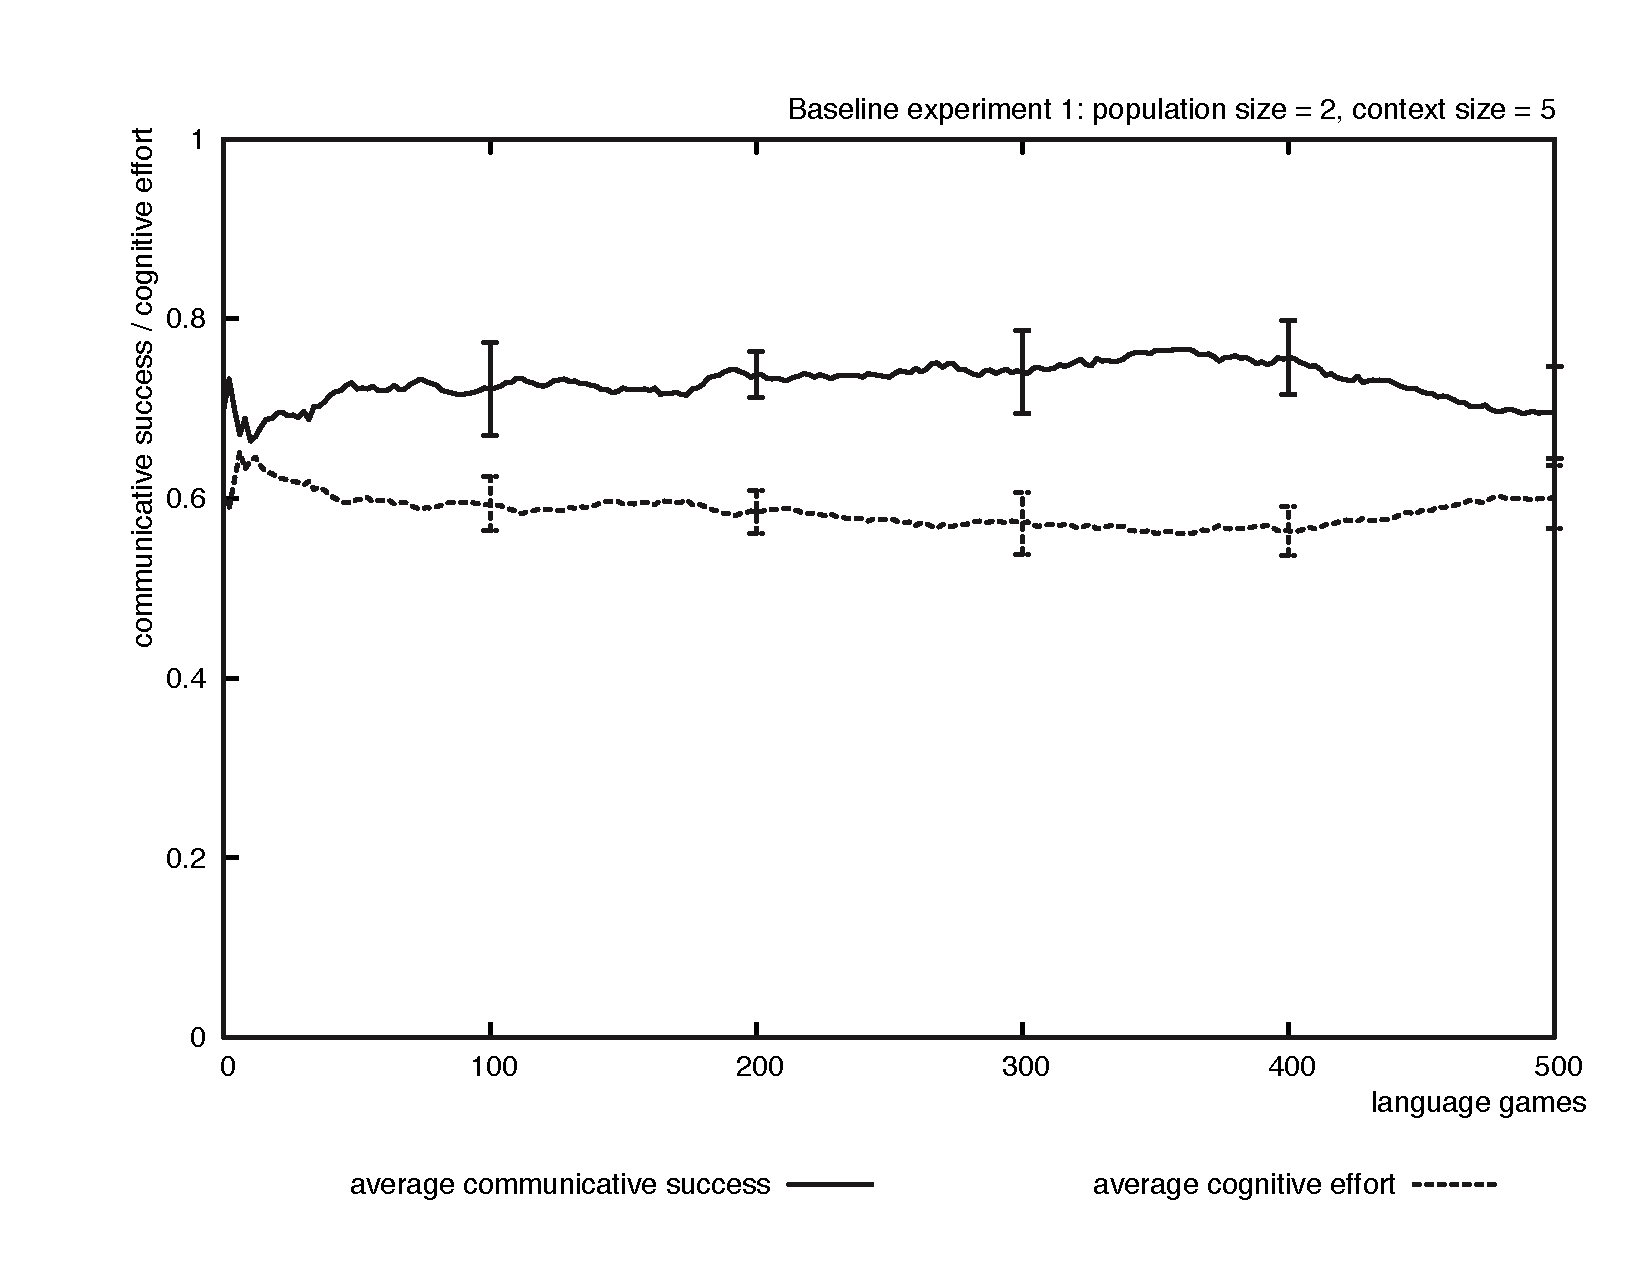
\includegraphics[width=\textwidth]{Chapter3/figs/graph-base1-effort2}}
  \caption[Baseline experiment 1: success and effort]{This graph shows the average cognitive effort\is{cognitive effort} and communicative success\is{communicative success} in baseline experiment 1 for 10 series of 500 language game\is{language game}s in a population\is{speech population} of two agents and a context size of five events. Success is reached in about 70\% of the games. Cognitive effort\is{cognitive effort} during interpretation amounts to 0,6 on average.}
   \label{f:base1-effort2}
\end{figure}


\subsubsection{Discussion}
 The results of baseline experiment 1 demonstrate that the agents can still reach communicative success\is{communicative success} if they use their world model for inferring the intended meaning. The proposed machinery thus works but only under certain conditions. For one thing, the hearer needs to have witnessed the scene in order to make the correct inferences. Second, the context cannot be too ambiguous otherwise interpretation can involve multiple hypotheses. As can be read from the average communicative success\is{communicative success} measure, this happens in 30\% of the cases. Failed games typically occur when the scene contains at least two event token\is{event token}s which have the same event type\is{event type} but which involve different participants.

Improving communicative success\is{communicative success} in the failed games could be achieved in many ways: agents can be given more complex dialogue\is{dialogue} strategies, the speaker can use pointing, the hearer can be more bold in making assumption\is{assumption}s about the speaker's intention or ask for additional feedback, etc. These strategies would however involve more negotiat\is{negotiation}ion and do not reduce the cognitive load during interpretation for the hearer. Additional marking, however, would be a solution which could resolve ambiguity\is{ambiguity} and reduce cognitive effort\is{cognitive effort} during interpretation at the same time. This solution will be tested in the next baseline experiment.

\section{Baseline experiment 2: specific marking}
\label{s:base2}

Baseline experiment 1 showed how agents can still reach communicative success\is{communicative success} without using grammar. In the second baseline experiment, agents can exploit this ability to autonomously detect whether it might be useful to make changes to their linguistic inventor\is{linguistic inventory}ies in order to optimize communication. The hypothesis investigated here can be formulated as follows: {\bfseries ambiguity\is{ambiguity} or too much cognitive effort\is{cognitive effort} during parsing and interpretation can be a trigger for the invention of functional marker\is{case!case marking}s for optimizing communicative success\is{communicative success}}.

\subsection{Speaker-based innovat\is{innovation}ion}

\begin{figure}[t]
\centerline{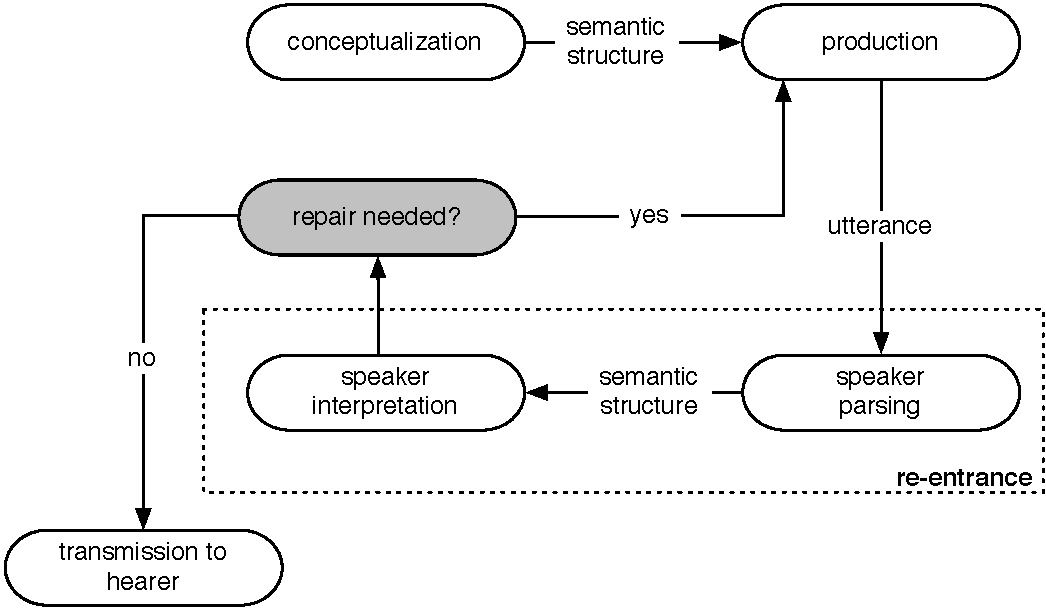
\includegraphics[width=\linewidth]{Chapter3/figs/re-entrance}}
  \caption[Speaker re-entrance]{Before transmitting an utterance to the hearer, the speaker `re-enters' her own utterance in her language system and uses herself as a model of the hearer. In this way the speaker estimates whether there might be problems or too much complexity for the hearer during parsing. If so, the speaker tries to repair\is{learning strategies!repair strategies} the problem.}
   \label{f:re-entrance}
\end{figure}

In baseline experiment 1 the hearer is faced with the cognitive load of figuring out who's doing what in events during each interaction. Moreover, if the context is complex enough it may not be clear which event the speaker was referring to. In this experiment, the agents are therefore endowed with a second key cognitive ability which involves the {\bfseries innovat\is{innovation}ion and expansion} of their language through event-specific marker\is{case!case marking}s. This ability comprises three subparts:

\begin{enumerate}
\item Expanding the agents architecture with a `re-entrant' mapping for detecting opportunities for optimization and learning innovat\is{innovation}ions;
\item Endowing the agents with the capacity of inventing a marker\is{case!case marking} and the corresponding constructions;
\item Endowing the agents with a consolidation\is{consolidation} mechanism which allows them to converge on a shared set of marker\is{case!case marking}s.  
\end{enumerate}

\subsubsection{Re-entrance\is{re-entrance}}
 In baseline experiment 1, the agents could confidently use their lexical items to communicate with each other since the lexicon\is{lexicon} in this model is fixed, unambiguous, and shared by all the agents. However, should this scaffold\is{scaffold} be taken away, the agents would have to worry about whether the words they use are also known and understood by the other agents. They would thus somehow have to be capable of predicting the parsing and interpretation behaviour of the hearer in order to increase the chances of reaching communicative success\is{communicative success}. This can be achieved through `re-entrance\is{re-entrance}' 
\citep{steels03language} -- also called the `obverter' strategy by \citet{smith03intelligent}.

Re-entrance\is{re-entrance} can be thought of as self-monitoring\is{monitoring} in which the speaker does not directly transmit his utterance to the hearer, but first `re-enters' the utterance into his own linguistic system and parses and interprets the utterance himself as if he was the hearer. By taking himself as a model to simulate the linguistic behaviour of the hearer, the speaker can detect whether there might be problems or difficulties during parsing and interpretation. If so, the speaker will try to solve this problem. This strategy is illustrated in Figure \ref{f:re-entrance}. Similarly, the hearer can also use a re-entrant mapping for simulating the behaviour of the speaker. Technically speaking, achieving re-entrance\is{re-entrance} is not so difficult since the agents in these experiments can act both as a speaker and as a hearer.

Re-entrance\is{re-entrance} is thus a crucial strategy in inferential coding system\is{inferential coding system}s: if the speaker wants to solve a problem through innovat\is{innovation}ion, he needs to have an educated guess about the hearer's knowledge and which aspects of the common ground can be exploited for getting the message across. The hearer has to perform the same kind of reasoning for guessing the speaker's intentions. Human language users obviously adapt their linguistic behaviours to their speech partners (e.g. when speaking to children or second language learners). Given the fact that all agents in the experiments are each other's peers, the best model they can have of other agents is themselves.


\subsubsection{Innovation}
 It is unavoidable that language users come across situations in which the speaker does not know an adequate and well-entrench\is{entrenchment}ed convention\is{convention} for expressing a certain meaning, especially in the extreme case where there is no grammar at all. In this experiment, the speaker will invent a specific marker\is{case!case marking} for explicitly expressing a particular participant role\is{participant role} if there are possible ambiguities in the context or if the hearer needs to do more inference than is desirable. This is implemented through {\bfseries diagnostic\is{learning strategies!diagnostics}s and repair\is{learning strategies!repair strategies} strategies} which run in this experiment along the following algorithm:

\begin{enumerate}
\item {\bfseries Diagnostic 1:} Re-enter the utterance into the linguistic system and start a parsing and interpretation task.
\begin{enumerate}
\item[a.] If interpretation returns a failure or multiple hypotheses, report a problem;
\item[b.] If there is one possible hypothesis which contains at least one unexpressed variable equal\is{variable equality}ity, report a problem;
\item[c.] If there is no inference needed and if there is only one hypothesis, transmit the utterance to the hearer.
\end{enumerate}
\item {\bfseries Repair strategy 1:} If a problem of ambiguity\is{ambiguity} or unresolved variable equal\is{variable equality}ities has been reported, trigger repair\is{learning strategies!repair strategies} strategy 1.
\begin{enumerate}
\item[a.] If there is only one unexpressed variable equal\is{variable equality}ity, invent a new marker\is{case!case marking} for it and start a new production task;
\item[b.] If there are more than one unexpressed variable equal\is{variable equality}ities left (i.e. the repair\is{learning strategies!repair strategies} is too difficult), ignore the problem and transmit the utterance to the hearer.
\end{enumerate}
\end{enumerate}

I will now illustrate this algorithm with a concrete example. Suppose that the speaker and hearer both observe the same scene as the one used in section \ref{s:base1} in which Jack was walking to Jill; and that the sensory-motor processing delivers the same facts as in example \ref{facts}. This time the speaker only profiles the part of the event involving Jack and conceptualizes the following meaning:

\ea
\begin{lstlisting}
(jack object-1)
 (walk-to event-1 true)
 (walk-to-1 event-1 object-1)
 (walk-to-2 event-1 object-2)
\end{lstlisting}
\z

Since the speaker has no grammar yet, only the lexical entr\is{lexical entry}ies of {\em Jack} and {\em walk-to} are unified and merged with the coupled feature structure\is{feature structure!coupled feature structure} which results in the following, randomly ordered utterance:

\ea
``jack walk-to''
\z

Instead of directly transmitting the utterance to the hearer, the speaker first re-enters the utterance into her own linguistic system and parses the following meaning:

\ea
\begin{lstlisting}
(jack ?object-a)
 (walk-to ?event-1 true)
 (walk-to-1 ?event-x object-x)
 (walk-to-2 ?event-x object-y)
\end{lstlisting}
\z

Interpreting this meaning by unify\is{unify and merge}ing it with the speaker's world model yields the following set of bindings:

\ea
\begin{lstlisting}
((?event-x . event-1) (?object-x . object-1)
  (?object-y . object-2) (?object-a . object-1))
\end{lstlisting}
\z

Unification is successful and returns only one hypothesis so the speaker does not detect ambiguity\is{ambiguity}. However, there is a variable equal\is{variable equality}ity left between the variable `?object-x' and `?object-a': both refer to `object-1'. {\bfseries Diagnostic 1 will therefore report a problem that triggers repair\is{learning strategies!repair strategies} strategy 1}.

The repair\is{learning strategies!repair strategies} strategy assesses the difficulty of the problem: if there are more than one unexpressed variable equal\is{variable equality}ities left, the problem is classified as `too difficult to solve' and then the utterance is transmitted anyway. Here, however, there is only one variable equal\is{variable equality}ity so the speaker will invent a new marker\is{case!case marking} for it. This marker\is{case!case marking} is specific to the walk-to-1 role and can thus almost be seen as a lexical item itself. The speaker then invents a {\bfseries verb\is{verb}-specific construction\is{construction!verb-specific construction}} in which the new marker\is{case!case marking} (let's say {\em -bo}) binds the referent of the walk-to-1-role to the referent of the argument that fills this role by using the same variable `?object-x'. The syntactic pole states that this argument plays `syn-role-1' which is nothing more than a direct mapping of the walk-to-1-role.


\ea
\begin{lstlisting}
<Construction: construction-1
 ((?unit-1
   (meaning (== (walk-to ?event-x ?truth)
                (walk-to-1 ?event-x ?object-x)
                (walk-to-2 ?event-x ?object-y))))
  (?unit-2
   (referent ?object-x)))
<==>
 ((?unit-2
   (syn-role syn-role-1)))>
\end{lstlisting}
\z


The morphological rule states that the marker\is{case!case marking} immediately follows the argument which plays the walk-to-1-role. As explained in the previous Chapter, the morphological rule will create a new marker\is{case!case marking}-unit and make it a sub-unit of the argument-unit. Both the verb\is{verb}-specific construction\is{construction!verb-specific construction} and the morph-rule look slightly different from the original proposals by \citet{steels02simulating} due to changes in the grammar formalism, but they have the same performance\is{performance}.


\ea
\begin{lstlisting}
<Morph-rule: -bo
 ((?top-unit
   (syn-subunits (== ?unit-1)))
  (?unit-1
   (syn-role syn-role-1)))
<==>
 ((?top-unit
   (form (== (string ?marker-unit "-bo")
            (meets ?unit-1 ?marker-unit))))
  ((J ?marker-unit ?top-unit))
  ((J ?unit-1 ?top-unit (?marker-unit))))>
\end{lstlisting}
\z


The speaker now starts a new production task for the same meaning. In the initial node in the reaction network\is{reaction network}, the whole meaning is still grouped together in one unit. The speaker then unifies and merges the lexical entr\is{lexical entry}ies of {\em jack} and {\em walk-to} with the initial node which leads to a separate unit for each word. The new coupled feature structure\is{feature structure!coupled feature structure} looks as follows:


\ea
\begin{lstlisting}
<Node-2: coupled-feature-structure
 ((top-unit
   (sem-subunits (jack-unit walk-to-unit)))
  (jack-unit
   (meaning ((jack object-1)))
   (referent object-1))
  (walk-to-unit
   (referent event-1))
   (meaning ((walk-to event-1 true)
              (walk-to-1 event-1 object-1)
              (walk-to-2 event-1 object-2))))
<==>
 ((top-unit
   (syn-subunits (jack-unit walk-to-unit)))
  (jack-unit
   (form ((string jack-unit ''jack''))))
  (walk-to-unit
   (form ((string walk-to-unit "walk-to")))))>
\end{lstlisting}
\z


Before the repair\is{learning strategies!repair strategies}, this would be the final node in the reaction network\is{reaction network}. This time, however, the speaker has the newly made construction at her disposal. Since this is a production task, the semantic pole of the construction needs to unify\is{unify and merge} with the semantic pole of node-2. This is successful: the construction needs any unit containing the meaning of a walk-to-event and another unit of which the referent is the same one as the referent of the walk-to-1-role (`object-1'). The syntactic pole of the construction then simply merges the feature-value pair `(syn-role syn-role-1)' to the argument-unit. The construction thus license\is{license}s the following node in the reaction network\is{reaction network}:


\ea
\begin{lstlisting}
<Node-3: coupled-feature-structure
 ((top-unit
   (sem-subunits (jack-unit walk-to-unit)))
  (jack-unit
   (meaning ((jack object-1)))
   (referent object-1))
  (walk-to-unit
   (referent event-1))
   (meaning ((walk-to event-1 true)
              (walk-to-1 event-1 object-1)
              (walk-to-2 event-1 object-2))))
<==>
 ((top-unit
   (syn-subunits (jack-unit walk-to-unit)))
  (jack-unit
   (syn-role syn-role-1)
   (form ((string jack-unit ''jack''))))
  (walk-to-unit
   (form ((string walk-to-unit "walk-to")))))>
\end{lstlisting}
\z


Next, the speaker can unify\is{unify and merge} and merge the new morph-rule with node-3. The left-pole of the morph-rule (which is syntactic, see section \ref{s:morph-rule}) looks for any unit containing the feature-value pair `(syn-role syn-role-1)' which is indeed present in the syntactic pole of node-3. Next, the right-pole of the morph-rule is merged with the right-pole of node-3:


\ea
\begin{lstlisting}
<Node-4: coupled-feature-structure
 ((top-unit
   (sem-subunits (jack-unit walk-to-unit)))
  (jack-unit
   (meaning ((jack object-1)))
   (referent object-1))
  (walk-to-unit
   (referent event-1))
   (meaning ((walk-to event-1 true)
              (walk-to-1 event-1 object-1)
              (walk-to-2 event-1 object-2))))
<==>
 ((top-unit
   (syn-subunits (jack-unit walk-to-unit)))
  (jack-unit
   (syn-subunits (bo-unit))
   (syn-role syn-role-1)
   (form ((string jack-unit ''jack''))))
  (bo-unit
   (form ((string bo-unit ''-bo'') (meets jack-unit bo-unit))))
  (walk-to-unit
   (form ((string walk-to-unit "walk-to")))))>
\end{lstlisting}
\z


The speaker has no other items that can be unified and merged so node-4 is the final node in the reaction network\is{reaction network}. The speaker then renders the form-features of the syntactic pole into an utterance. The ordering between the words {\em jack} and {\em walk-to} are still random, but the coupled feature structure\is{feature structure!coupled feature structure} specifies that the marker\is{case!case marking} {\em -bo} immediately follows {\em jack}. This results in the following utterance:

\ea
``jack -bo walk-to''
\z

The speaker now re-enters this utterance again into his linguistic system to check whether the innovat\is{innovation}ion has the intended effect. I will not repeat the entire trace of parsing here since this is completely analog\is{analogy}ous to the example given in Chapter \ref{c:ar}. Parsing the utterance yields the following meaning:

\ea
\begin{lstlisting}
(jack ?object-x)
 (walk-to ?event-x true)
 (walk-to-1 ?event-x object-x)
 (walk-to-2 ?event-x object-y)
\end{lstlisting}
\z

Note that this time, the meaning-predicates `jack' and `walk-to-1' share the same variable `?object-x'. Interpretation then returns the following set of bindings:

\ea
{\footnotesize\tt{((?event-x . event-1) (?object-x . object-1) \\ \hspace{3,3mm}(?object-y . object-2))}}
\z

As can be seen in the set of bindings, there are no unexpressed variable equal\is{variable equality}ities left so no additional inferences are needed. The speaker is thus satisfied with the utterance and transmits it to the hearer.


\subsubsection{Learning}
 Learning a new marker\is{case!case marking} is very similar to inventing one and is achieved through the same cognitive mechanisms. The hearer first observes the utterance and then parses it. If there are unknown strings, such as the marker\is{case!case marking} {\em -bo} which was just invented by the speaker, the hearer will ignore it and try to parse as much as possible. Then the hearer tries to interpret the parsed meaning. If there are unexpressed variable equal\is{variable equality}ities left, the same diagnostic\is{learning strategies!diagnostics} as was used by the speaker will report a problem. The repair\is{learning strategies!repair strategies} strategy then tries to find out whether the utterance contains elements which could carry this particular meaning or function.

\begin{enumerate}
\item {\bfseries Hearer diagnostic\is{learning strategies!diagnostics} 1:} Parse the utterance and interpret its meaning.
\begin{enumerate}
\item[a.] If interpretation returns a failure or multiple hypotheses, report a problem;
\item[b.] If there is one possible hypothesis which contains at least one unexpressed variable equal\is{variable equality}ity, report a problem;
\item[c.] If there is no inference needed and there is only one hypothesis, signal agreement to the speaker.
\end{enumerate}
\item {\bfseries Hearer repair\is{learning strategies!repair strategies} strategy 1:} If a problem of ambiguity\is{ambiguity} or unresolved variable equal\is{variable equality}ities has been reported, trigger repair\is{learning strategies!repair strategies} strategy 1.
\begin{enumerate}
\item[a.] If there is only one unexpressed variable equal\is{variable equality}ity, check whether there was one unknown string in the utterance. If so, add a new verb\is{verb}-specific construction\is{construction!verb-specific construction} to the inventory which records the unknown string as a marker\is{case!case marking} for the variable equal\is{variable equality}ity. If not, ignore the problem and signal agreement or disagreement to the speaker depending on success of the game;
\item[b.] If there are more than one unexpressed variable equal\is{variable equality}ities left or if there were multiple unknown strings, ignore the problem. Transmit success to the hearer if inference is nevertheless possible. 
\item[c.] If interpretation fails or leads to multiple hypotheses, ignore the problem and signal disagreement.
\end{enumerate}
\end{enumerate}

\subsubsection{Consolidation\is{consolidation}}
 In the original two-agent simulations variety never occurs since the agents only observe each other's inventions except for the extremely rare cases in which the learning task was too difficult and the learner later on invents a different solution for the same problem. So consolidation\is{consolidation} is fairly trivial and means just storing the newly created or learned items in the linguistic inventor\is{linguistic inventory}y.

However, as soon as we scale up the experiments to multi-agent population\is{speech population}s involving at least three agents, a pool of synchron\is{synchronic}ic variation\is{variation} naturally arises since the agents can independently come up with different innovat\is{innovation}ions for the same problems. The agents therefore need to have an alignment strateg\is{alignment strategy}y that enables them to deal with the variety and to converge on a shared set of preferred marker\is{case!case marking}s.

\begin{figure}[htp]
\centerline{\begin{tabular}{c}
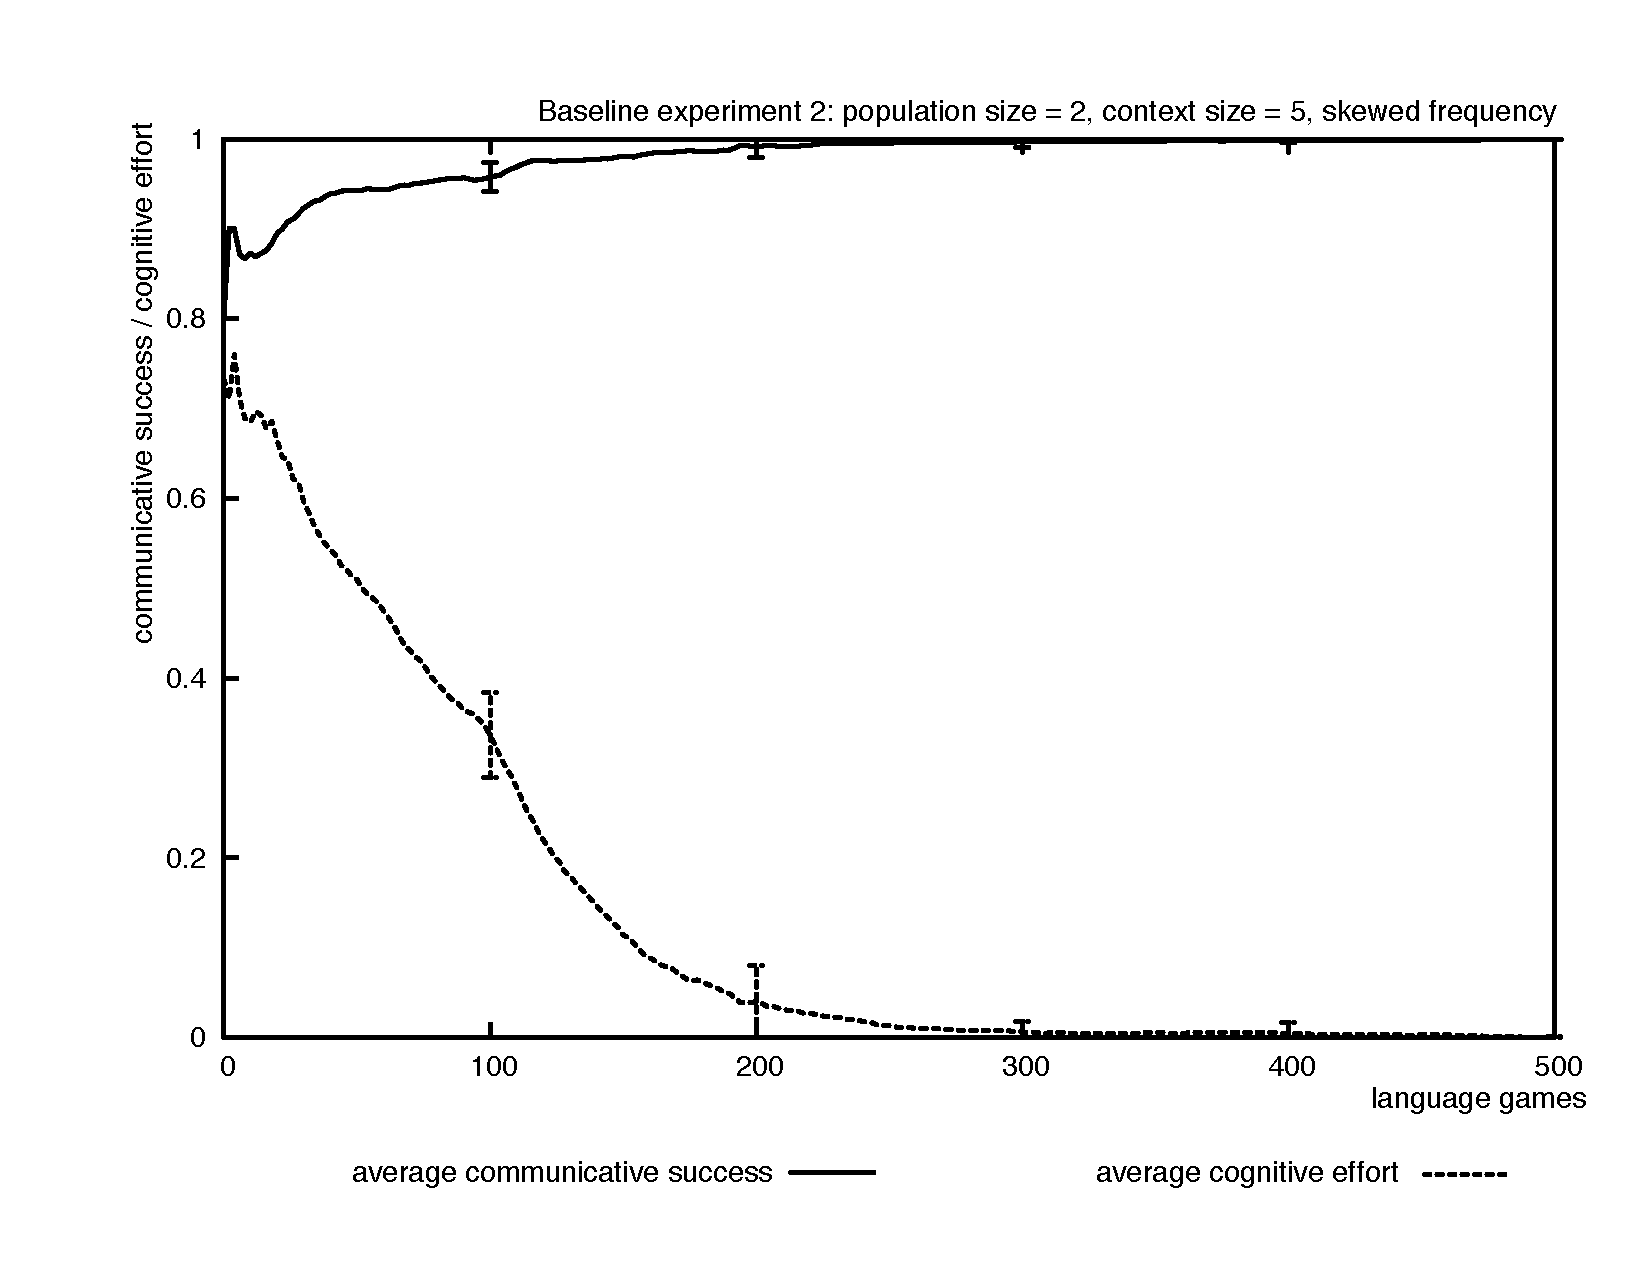
\includegraphics[width=0.8\linewidth]{Chapter3/figs/graph-base2-effort}
 \\
 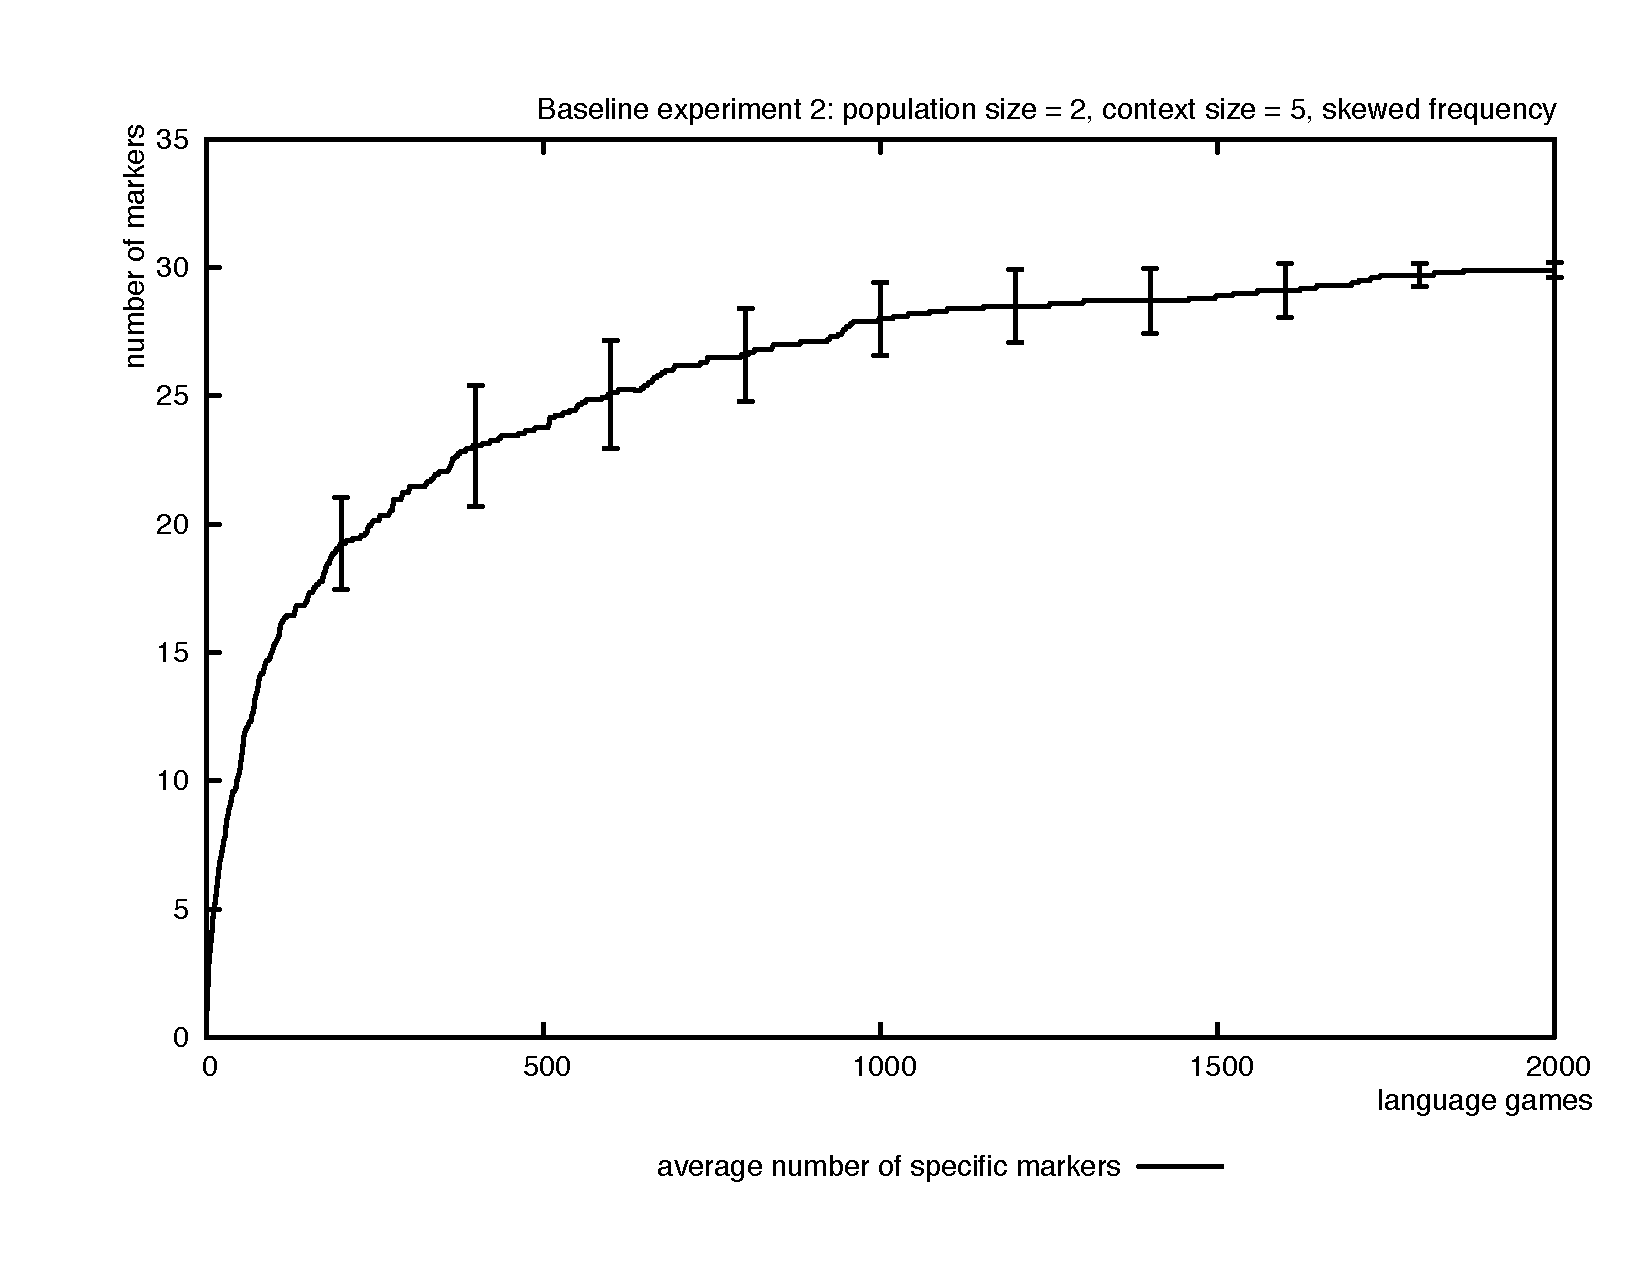
\includegraphics[width=0.8\linewidth]{Chapter3/figs/graph-base2-size}
  \end{tabular}}
  \caption[Baseline experiment 2: replication]{The top graph shows that the agents rapidly reach 100\% communicative success\is{communicative success} in the two-agent set-up. The agents also succeed in reducing the cognitive effort\is{cognitive effort} to zero. The bottom graph shows that they need to learn and store 30 specific marker\is{case!case marking}s in their inventory to do so.}
\label{f:base2-effort}
\end{figure}

In section \ref{s:towards-grammar} I argued that the experiments on grammar first of all try to move all the previous work on lexicon\is{lexicon} formation onto the domain of grammar, so this experiment starts with a similar alignment strateg\is{alignment strategy}y as was suggested in prior work. This strategy goes as follows: each construction has its own {\bfseries confidence\is{confidence} score} between 0 and 1. The higher the score, the more confident the agent is that the item is a convention\is{convention}alized unit in the population\is{speech population}. Based on the game's success and based on the speaker's behaviour, the hearer will update the scores in the inventory as follows:

\begin{itemize}
\item In case of success, increase the score of the applied construction(s) by 0.1 and decrease the scores of all its competit\is{competition}ors through {\bfseries lateral inhibition\is{lateral inhibition}} by 0.1. Competitors of a construction are constructions which either have the same semantic pole but a different form (competing synonyms), or the same form but different semantics (competing homonyms);
\item If the game was a failure, do nothing.
\end{itemize}

The fact that only the hearer performs score updating captures the intuition that agents first of all want to {\bfseries conform to} the behaviours of other agents in the population\is{speech population} rather than imposing their own preferences. A mathematical model by \citet{devylder07evolution} also shows that this strategy results in smoother convergence dynamics. In case of game failure, neither the speaker nor the hearer updates any scores. The reason for this is that the description game\is{language game!description game} does not offer enough explicit feedback for the agents to find out whether there might be parts in the processing chain which were harmful for communication.

\subsection{Results and discussion}

The above diagnostic\is{learning strategies!diagnostics}s and repair\is{learning strategies!repair strategies} strategies have been implemented and tested in three different simulations. The first series (set-up 2a) features a population\is{speech population} of two agents and replicates the results obtained by \citet{steels02simulating, steels04constructivist}. The second experiment (set-up 2b) involves a population\is{speech population} of ten agents in which the consolidation\is{consolidation} strategies become necessary for convergence. Both experiments feature the skewed frequency\is{frequency} of event type\is{event type}s mentioned in section \ref{s:world}. A third set-up (set-up 2c) also features 10 agents, but this time the skewed frequency\is{frequency} was replaced by an equal\is{variable equality} frequency\is{frequency} of event type\is{event type}s in order to study the convergence and competit\is{competition}ion dynamics more easily. All the results were obtained after ten series of language game\is{language game}s for each simulation.


\begin{figure}[phtb]
\centerline{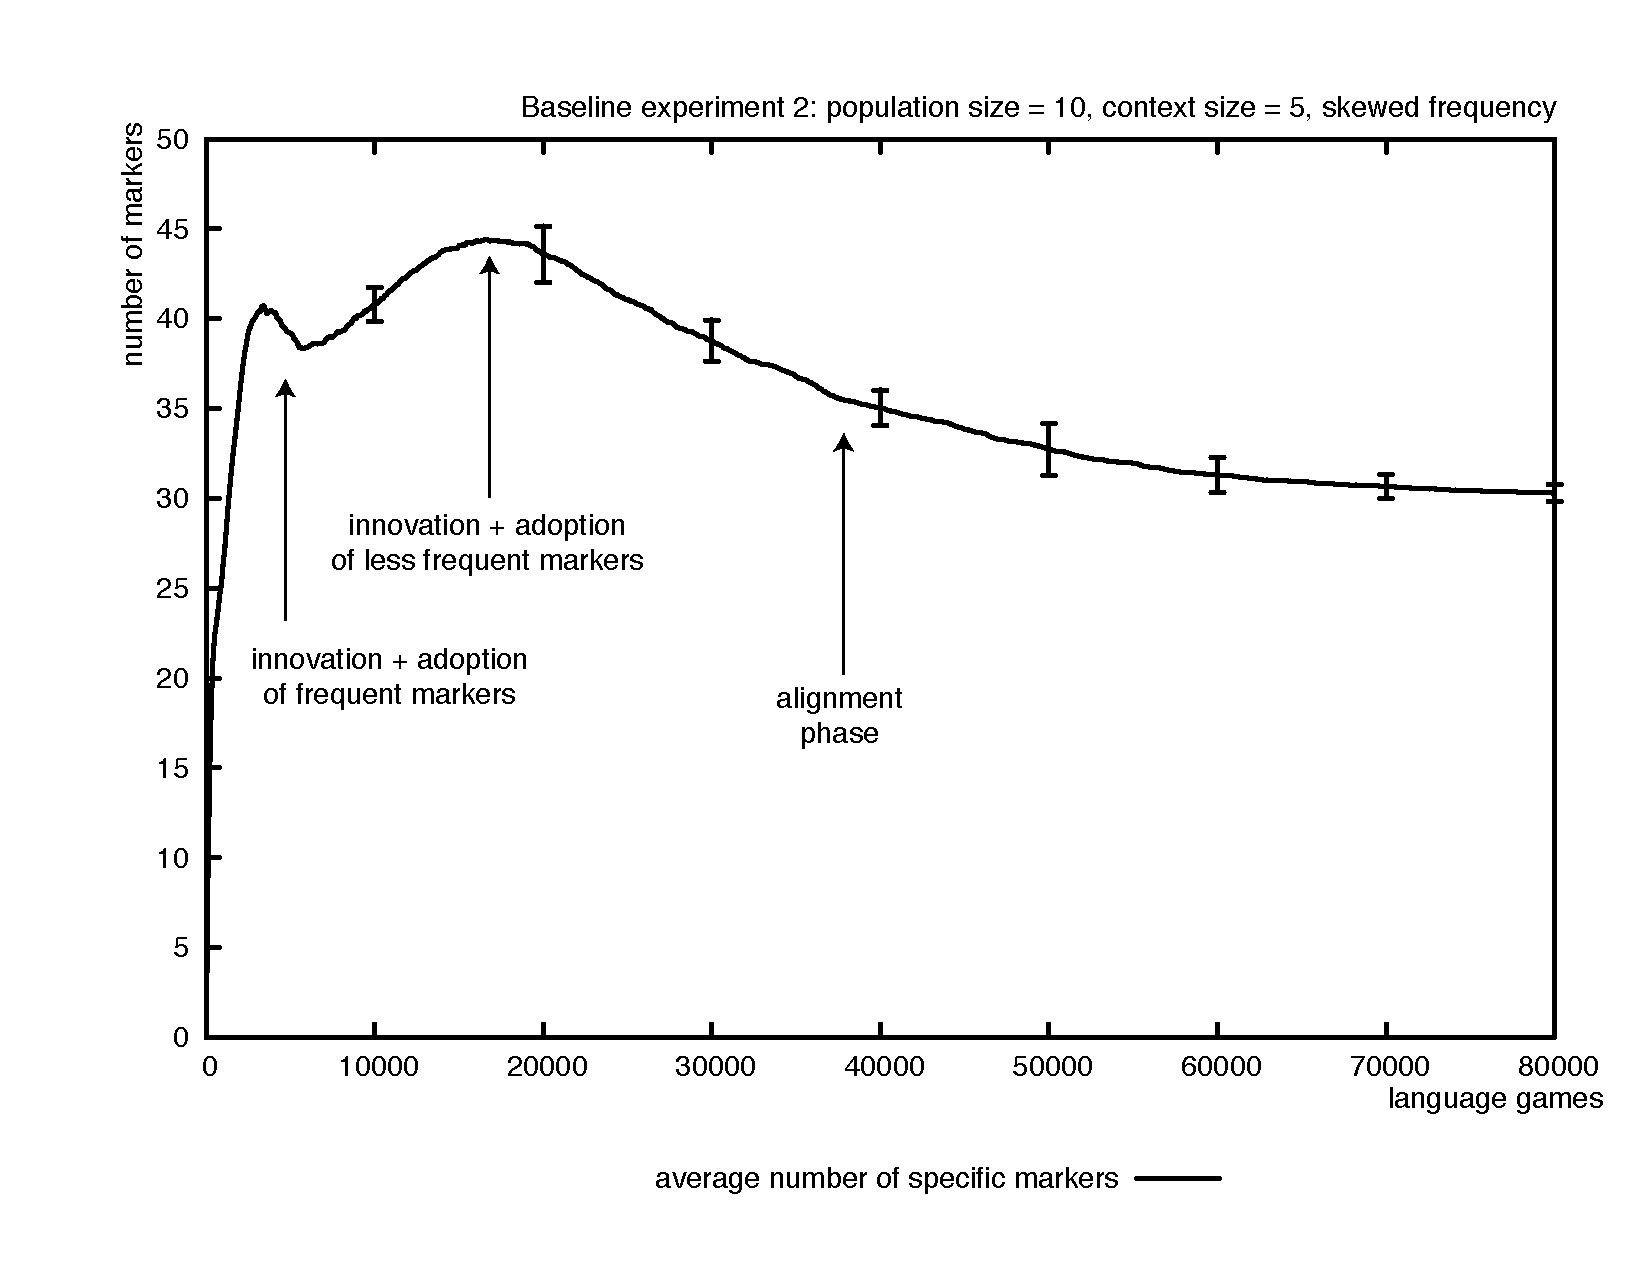
\includegraphics[width=\textwidth]{Chapter3/figs/graph-base2-size1}}
  \caption[Baseline experiment 2: number of markers (skewed frequency\is{frequency})]{This graph shows the number of specific marker\is{case!case marking}s in baseline experiment 2b for 10 series of 80.000 language game\is{language game}s in a population\is{speech population} of 10 agents and a context size of five events. The agents start innovat\is{innovation}ing and learning marker\is{case!case marking}s rapidly during the first 3.000 games after which a short period of alignment seems to kick in. The number of marker\is{case!case marking}s then rises again between game 7.000 and game 20.000. This is due to the skewed frequency\is{frequency} of the event-tyes: events that potentially take three participants are very rare in the data and marker\is{case!case marking}s for them are only now being acquired by all agents. Finally, a long alignment period starts which also takes much more time for the less-frequent event type\is{event type}s.}
   \label{f:base2-size1}
\end{figure}
\subsubsection{Results of set-up 2a}
 The results obtained from the replication experiment confirm the results of the original case experiment. The top graph in Figure \ref{f:base2-effort} shows that the average cognitive effort\is{cognitive effort} needed by the speaker rapidly drops to zero if the agents start inventing and using specific marker\is{case!case marking}s to indicate relations between events and their participants. With the marker\is{case!case marking}s the agents are also capable of overcoming ambiguity\is{ambiguity} in the context since communicative success\is{communicative success} rises to 100\%. However, there is a price to pay for this optimization, which is shown in the bottom graph: for each participant role\is{participant role}, the agents have to learn and store a specific marker\is{case!case marking} in the inventory. In this two-agent simulation, no variation\is{variation} occurs so agreeing on a set of 30 marker\is{case!case marking}s is fairly trivial.


\begin{figure}[ht]
\centerline{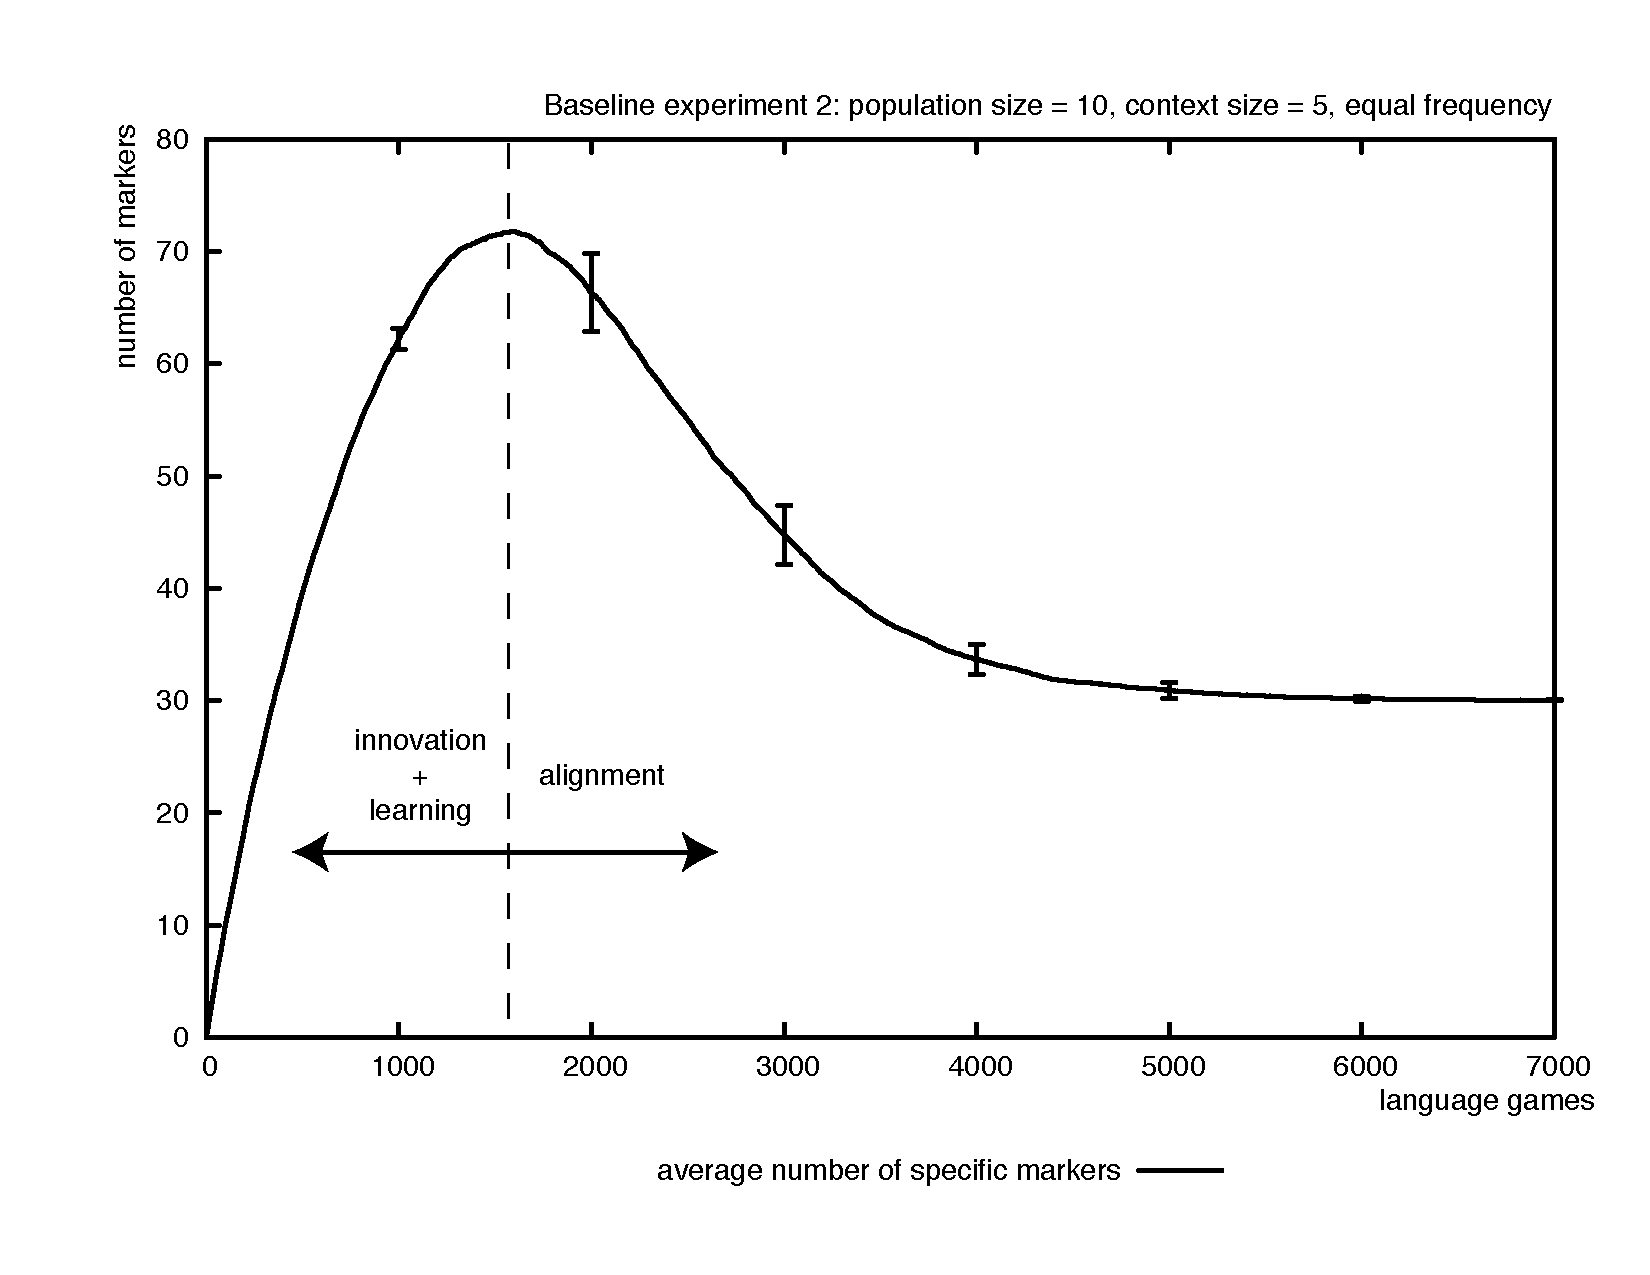
\includegraphics[width=0.8\textwidth]{Chapter3/figs/graph-base2-size2}}
  \caption[Baseline experiment 2c: number of markers (equal\is{variable equality} frequency\is{frequency})]{This graph shows the number of specific marker\is{case!case marking}s in baseline experiment 2c for 10 series of 7.000 language game\is{language game}s in a population\is{speech population} of 10 agents and a context size of five events. This case, all event type\is{event type}s occur with the same frequency\is{frequency} so we can see the convergence dynamics in the population\is{speech population} more clearly: agents invent and learn new marker\is{case!case marking}s during the first 1.500 language game\is{language game}s. The agents then need another 4.500 language game\is{language game}s in order to align their linguistic inventor\is{linguistic inventory}ies with each other.}
   \label{f:base2-size2}
\end{figure}
\subsubsection{Results of set-up 2b}
 If the population\is{speech population} size is increased, the agents need much more time to learn all the variation\is{variation}s floating in the population\is{speech population} and to converge on a shared set of 30 marker\is{case!case marking}s. As Figure \ref{f:base2-size1} shows, the agents need 80.000 language game\is{language game}s in order to agree on this set. This is still fairly rapid: it means that each agent needs to play an average of 8.000 games in order to conform to the language of its peers.

The graph first shows a steep rise to an average of 40 marker\is{case!case marking}s in the beginning after which an alignment phase seems to start. However, the number of marker\is{case!case marking}s starts to climb up again after 7.000 games and reaches a height of about 45 marker\is{case!case marking}s by the time 20.000 games have been played. Then there is a long and gradual slope towards convergence at 80.000 games. The two peaks in the graph are the result of the skewed frequency\is{frequency} of event type\is{event type} occurrences: marker\is{case!case marking}s for three-participant events are very rare and are therefore constructed, learned and propagat\is{propagation}ed later than the frequent marker\is{case!case marking}s. Even so, the agents still reach agreement and communicative success\is{communicative success} while reducing the cognitive effort\is{cognitive effort} needed if they are given enough time.


\begin{figure}[t]
\centerline{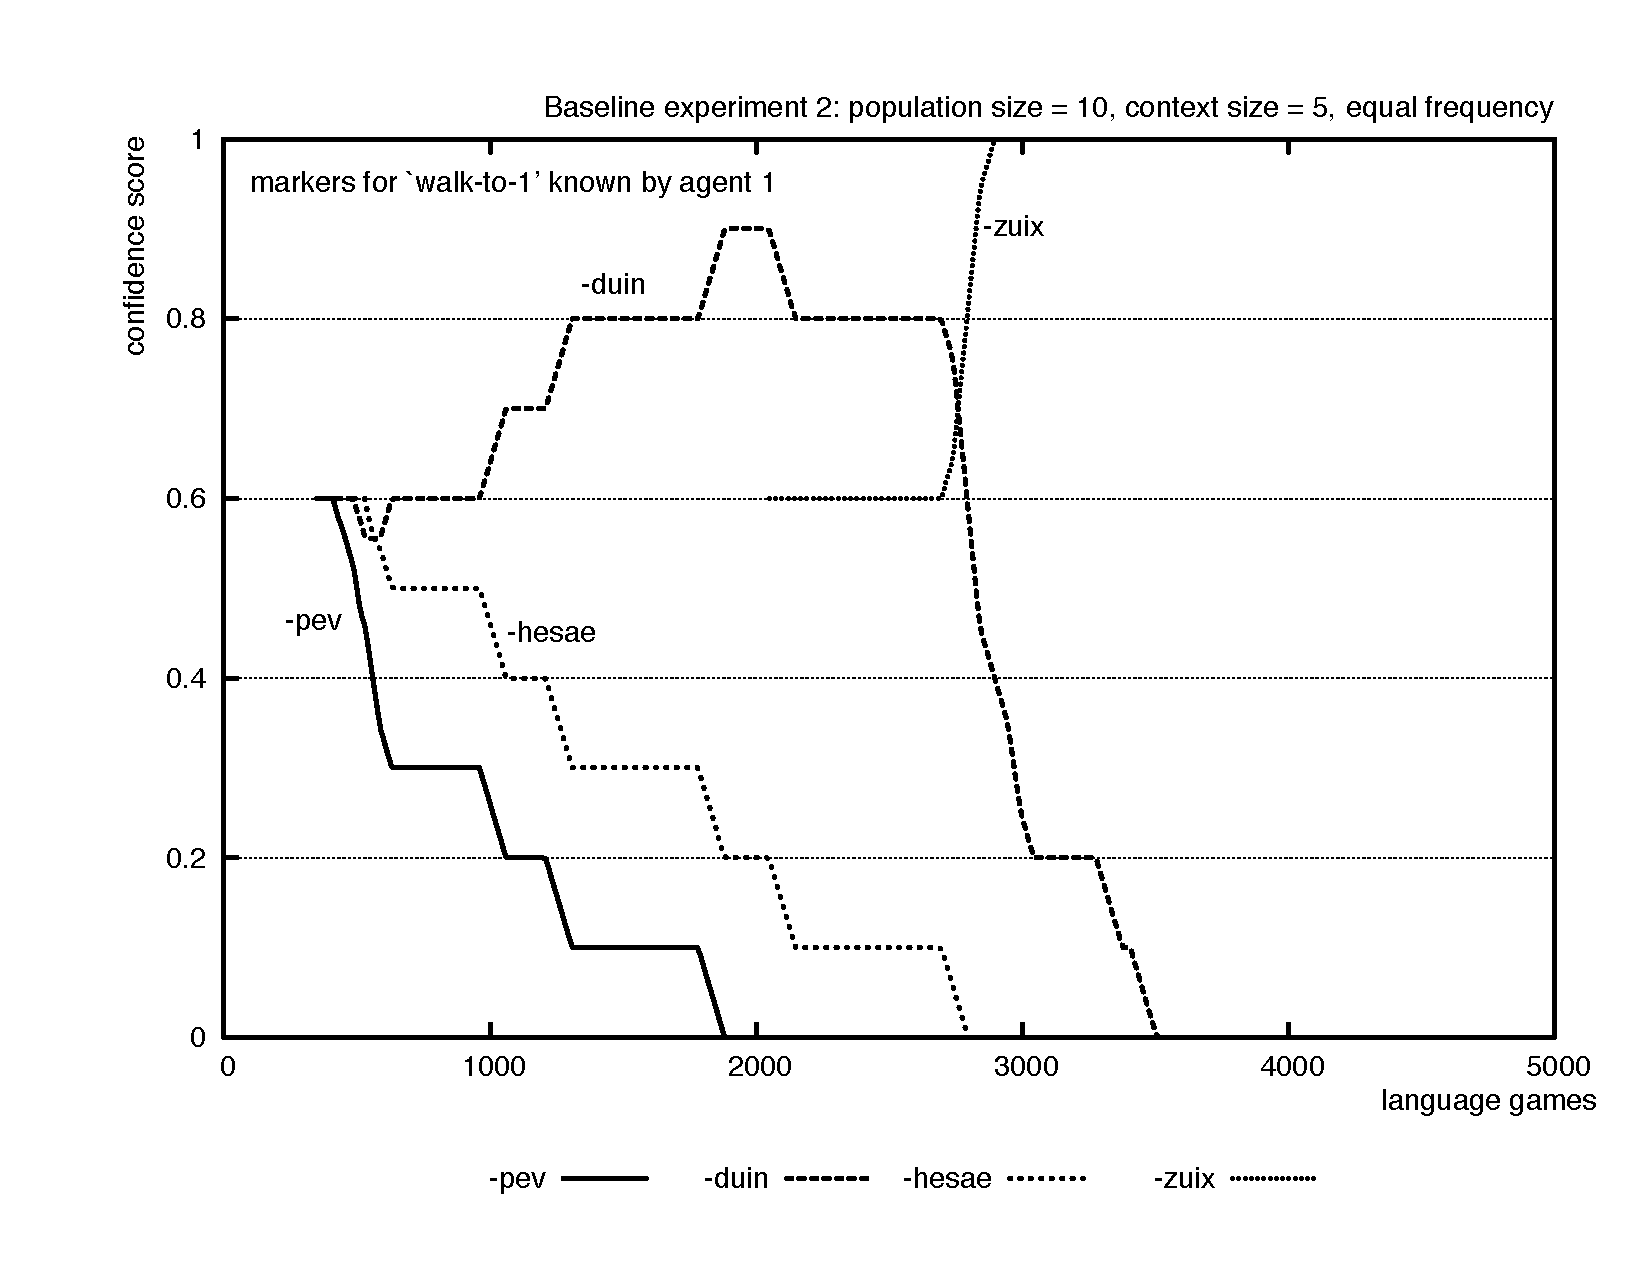
\includegraphics[width=0.87\textwidth]{Chapter3/figs/graph-base2-comp}}
  \caption[Baseline experiment 2: snapshot of competit\is{competition}ion (equal\is{variable equality} frequency\is{frequency})]{This graph shows a snapshot of the competit\is{competition}ion between forms for marking the participant role\is{participant role} `walk-to-1' within agent 1. Agent 1 learns the marker\is{case!case marking} {\em -pev} at first, but soon also observes {\em -duin} and {\em -hesae}. The marker\is{case!case marking} {\em -duin} seems to win the competit\is{competition}ion and even reaches a confidence\is{confidence} score of 0.9 after 2.000 language game\is{language game}s. However, the agent then learns another marker\is{case!case marking} {\em -zuix} which is apparently shared by a lot of other agents in the population\is{speech population}: at game 3.000 it has already pushed {\em -duin} down and it reaches 1.0 confidence\is{confidence} score.}
   \label{f:base2-comp}
\end{figure}
\subsubsection{Results of set-up 2c}
 In the third set-up all the event type\is{event type}s occur with the same frequency\is{frequency} so we can better study the convergence dynamics without other influences. Figure \ref{f:base2-size2} shows that the agents indeed need significantly less time than in the second set-up: between six and seven thousand language game\is{language game}s. On average this means about 600--700 games per agent, which comes close to the 500 games needed by the agents in two-agent simulations. The convergence task here is comparable in difficulty to a multiple word naming game\is{language game!multiword naming game} involving 30 objects \citep[see][]{vanlooveren05design}. The graph shows that the agents keep innovat\is{innovation}ing and learning new marker\is{case!case marking}s during the first 1.500 language game\is{language game}s after which they rapidly converge on a shared set of 30 marker\is{case!case marking}s. The peak of 70 marker\is{case!case marking}s -- as opposed to the peak of 45 with the skewed frequency\is{frequency} -- is normal since there are more competing marker\is{case!case marking}s floating in the population\is{speech population} at the same time.

Figure \ref{f:base2-comp} gives a snapshot of one agent's knowledge of marker\is{case!case marking}s for the participant role\is{participant role} `walk-to-1'. The agent learns three marker\is{case!case marking}s at about the same time: {\em -pev}, {\em -duin}, and {\em -hesae}. The marker\is{case!case marking} {\em -duin} seems to be the winning marker\is{case!case marking} and reaches a confidence\is{confidence} score of 0.9 by the time the agents have played 2.000 language game\is{language game}s. However, the agent then learns a new marker\is{case!case marking} {\em -zuix} which seems to be quite successful in the population\is{speech population}: its confidence\is{confidence} score rapidly increases to the maximum while {\em -duin} goes downhill very fast because of lateral inhibition\is{lateral inhibition}. In the end, {\em -zuix} wins the competit\is{competition}ion. 
\begin{figure}[t]
\centerline{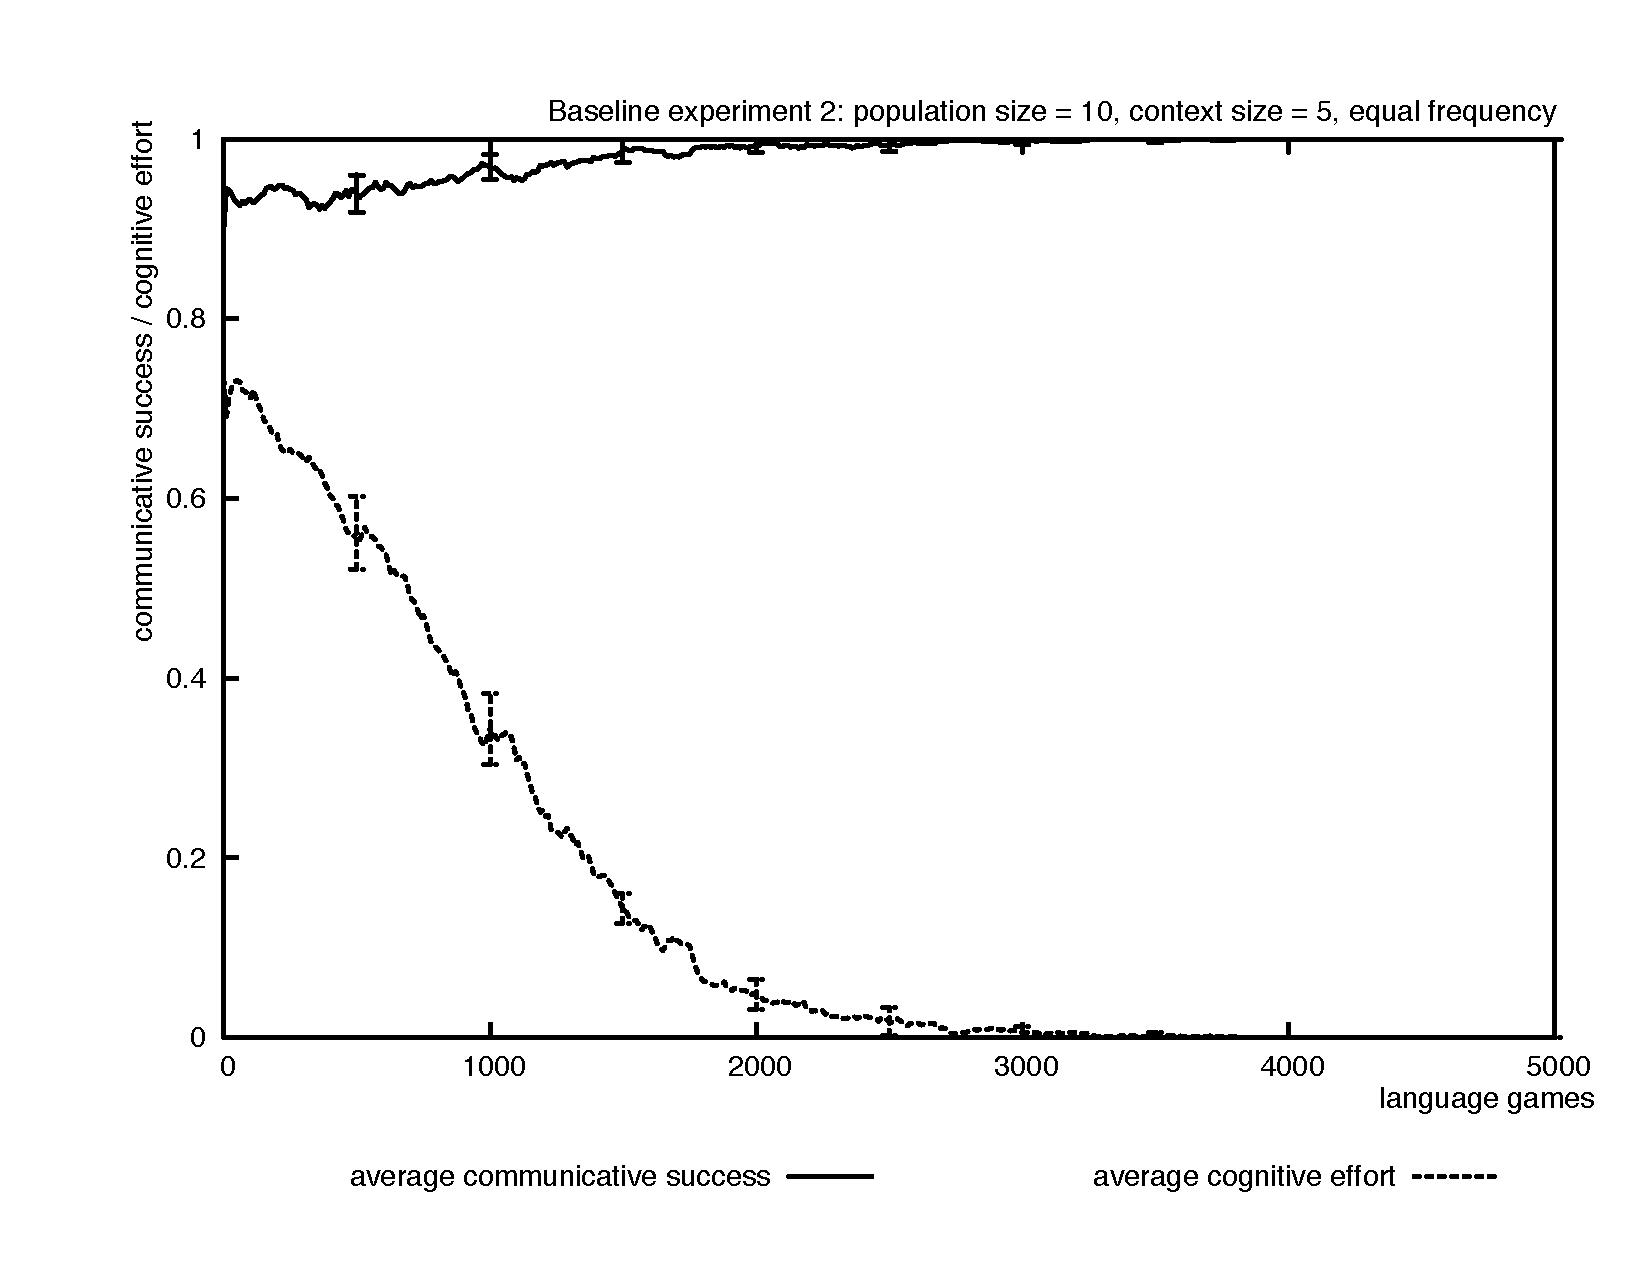
\includegraphics[width=\textwidth]{Chapter3/figs/graph-base2-effort2}}
  \caption[Baseline experiment 2: success and effort (equal\is{variable equality} frequency\is{frequency})]{In the multi-agent population\is{speech population}s too the agents succeed in reaching communicative success\is{communicative success} as well as reducing the cognitive effort\is{cognitive effort} needed for interpretation.}
   \label{f:base2-effort2}
\end{figure}

Finally, Figure \ref{f:base2-effort2} shows the average communicative success\is{communicative success} and cognitive effort\is{cognitive effort} again. The results show that the agents in the multi-agent simulations also rapidly reach 100\% communicative success\is{communicative success} by using marker\is{case!case marking}s. Cognitive effort\is{cognitive effort} also goes down until no inferences need to be made anymore.


\subsubsection{Discussion}
 The results of baseline experiment 2 clearly illustrate how agents can use locally available information\is{formation} to assess their own linguistic interactions and couple this assessment to repair\is{learning strategies!repair strategies} and consolidation\is{consolidation} strategies in order to improve communication. In this case, the agents mainly acted to reduce the semantic complexity of interpretation for the hearer: if additional marker\is{case!case marking}s are introduced for explicitly indicating the relations between events and their participants, parsing leads the agents immediately to the desired bindings in interpretation. Without the marker\is{case!case marking}s, additional inferences would still be needed.

However, a price has to be paid for reducing the effort of interpretation and that is an increased inventory size. During the language game\is{language game}s, the agents learn 70 marker\is{case!case marking}s on average and retain 30 of them, each one specific to a particular participant role\is{participant role}. The inventory size is in fact not the main problem here but a side-effect of a bigger issue: since the marker\is{case!case marking}s are restricted to one function only, the agents (given their present capabilities) cannot use them to go beyond the data of known events. Hence there is no generalization. Inventing new marker\is{case!case marking}s for each participant role\is{participant role} may be an efficient strategy in a small and fixed world, but becomes problematic once agents have to adapt to new meanings and communicative challenges.

Coupling these results back to natural languages, there are thus two clear qualitative differences: (a) marker\is{case!case marking}s in natural languages {\em do} generalize and become polysemous; and (b) they are not randomly invented but recruited from existing lexical items (see sections \ref{s:stage2} and \ref{s:stage3}). Both issues will have to be addressed in other experiments.


\section{Baseline experiment 3: semantic role\is{semantic role}s}
\label{s:base3}

The results of baseline experiment 2 indicate that the agents can reduce the problem of ambiguity\is{ambiguity} and cognitive effort\is{cognitive effort} if they make use of additional marking. However, the proposed innovat\is{innovation}ion strategy requires new marker\is{case!case marking}s to be invented all the time so (a) there is no generalization beyond the known data, and (b) this may lead to an explosion of the inventory size in the long run. Baseline 3 investigates how the same principles of diagnosis and repair\is{learning strategies!repair strategies} in order to reach communicative success\is{communicative success} can lead to generalization. The hypothesis is that {\bfseries analog\is{analogy}ical reasoning over event structure\is{event structure}s can account for an increased generalization and productivity\is{productivity} of case marker\is{case!case marking}s}.

\subsection{Generalization as a side-effect}

When repair\is{learning strategies!repair strategies}ing a problem of unexpressed variable equal\is{variable equality}ties in the previous baseline experiment, the speaker assessed the repair\is{learning strategies!repair strategies} to be too difficult to learn if the context was too ambiguous. In a more complex simulation, however, one can imagine that ambiguity\is{ambiguity} is rather the rule than the exception so the speaker needs to innovat\is{innovation}e in a more clever way to give the hearer additional clues about what he meant. One such strategy is to reuse\is{reuse} existing items as much as possible in semantically related or analog\is{analogy}ous situations. In baseline experiment 3, the speaker can reuse\is{reuse} the existing marker\is{case!case marking}s in new situations by performing analog\is{analogy}ical reasoning over event structure\is{event structure}s. The analog\is{analogy}y algorithm comprises the following steps:

\begin{enumerate}
\item Given a target participant role\is{participant role}$_{i}$, find a source role$_{j}$ for which a case marker\is{case!case marking} already exists;
\item Elaborate the mapping between the two:
\begin{enumerate}
\item[a.] Take the target event structure\is{event structure} in which participant role\is{participant role}$_{i}$ occurs (provided by sensory-motor processing);
\item[b.] Take the source event structure\is{event structure} of the event that was used to create source role$_{j}$;
\item[c.] Select from the source event structure\is{event structure} all the facts and micro-events involving the filler of source role$_{j}$ and retrieve the corresponding facts and micro-events of the target event structure\is{event structure}. 
\end{enumerate}
\item Keep the mapping if it is good. A good mapping means that:
\begin{enumerate}
\item[a.] the filler of source role$_{j}$ always maps onto the same object in the corresponding facts and micro-events;
\item[b.] the corresponding object fills the target role$_{i}$ in in the target structure.
\end{enumerate}
\item If there are multiple analog\is{analogy}ies possible, choose the best one (based on entrench\is{entrenchment}ment and category size);
\item Build the necessary constructions and make the necessary changes to existing items.
\end{enumerate}

Step 3b in the algorithm ensures that an analog\is{analogy}ical role is also discriminating enough to distinguish the target role from other possible participant role\is{participant role}s in the same or other events. By reusing\is{reuse} existing items in novel but similar situations, the speaker reduces the hypothesis space for the hearer and facilitates the abduction\is{abduction} process. The hearer can retrieve the analog\is{analogy}y using the same algorithm if he also knows the other marker\is{case!case marking}. In this strategy, the generalization of existing linguistic items is not a goal in itself but rather a side-effect of optimizing communicative success\is{communicative success}.


\subsubsection{The target and the source}
 I will illustrate the analog\is{analogy}y algorithm of this experiment through an example. Suppose that the speaker wants to construct a marker\is{case!case marking} for the participant role\is{participant role} `walk-to-2' of the following walk-to-event:

\ea
\begin{lstlisting}
(walk-to event-100 true) (walk-to-1 event-100 jack)
   (walk-to-2 event-100 jill)
\end{lstlisting}
\z

I will from now on refer to `walk-to-2' as the {\em target role} and to `jill' as the {\em target filler}. Instead of inventing a new marker\is{case!case marking} immediately, the speaker will first check whether he already knows a marker\is{case!case marking} which is analog\is{analogy}ous and hence could be reuse\is{reuse}d. Suppose that the speaker already knows the marker\is{case!case marking} {\em -mi} for the participant role\is{participant role} `move-inside-1'. I will from now on refer to this participant role\is{participant role} as the {\em source role} and its filler as the {\em source filler}. The speaker has stored the original event which he used for creating the marker\is{case!case marking} and retrieves it from his memory:

\ea
\begin{lstlisting}
 
(move-inside event-163190 true) 
(move-inside-1 event-163190 jill)
(move-inside-2 event-163190 house-1)
\end{lstlisting}
\z

\subsubsection{Elaborate the mapping between the two}
 In order to elaborate the mapping between the two events, the complete event structure\is{event structure} is taken. The target event (walk-to) consists of four micro-events: one participant is moving and approaching another participant, which stands still until the two participants touch each other:

\begin{itemize}
 \item
\begin{lstlisting}
(move event-165641 true) (move-1 event-165641 jack)
\end{lstlisting}
\item
\begin{lstlisting}
(move event-165419 false) (move-1 event-165419 jill)
\end{lstlisting}
\item
\begin{lstlisting}
(approach event-165486 true) (approach-1 event-165486 jack)
(approach-2 event-165486 jill)
\end{lstlisting}
\item
\begin{lstlisting}
(touch event-165633 true) (touch-1 event-165633 jill)
(touch-2 event-165633 jack) 
\end{lstlisting}
\end{itemize}

 

The source event (move-inside) is made up of eight micro-events. The event starts with two visible participants, of which one is standing still. The distance between both objects becomes smaller as one participant moves to the other. This continues until they `touch' each other after which the moving participant disappears out of sight.

\begin{itemize}
\item \begin{lstlisting}
(visible event-161997 true) (visible-1 event-161997 jill)
\end{lstlisting}

\item \begin{lstlisting}
(visible event-161791 true) (visible-1 event-161791 house-1)
\end{lstlisting}

\item 
\begin{lstlisting}
(move event-161794 false) (move-1 event-161794 house-1)
\end{lstlisting}


\item\begin{lstlisting}
(distance-decreasing event-162441 true)
(distance-decreasing-1 event-162441 jill)
(distance-decreasing-2 event-162441 house-1)
\end{lstlisting}

\item 
\begin{lstlisting}
(touch event-161801 false) (touch-1 event-161801 jill)
  (touch-2 event-161801 house-1)
\end{lstlisting}

\item \begin{lstlisting}
(touch event-162493 true) (touch-1 event-162493 jill)
  (touch-2 event-162493 house-1)
\end{lstlisting}

\item\begin{lstlisting}
(borderscreen event-162377 false) (object-1 event-162377 jill)
\end{lstlisting}

\item \begin{lstlisting}
(visible event-162665 false) (visible-1 event-161997 jill)
\end{lstlisting}
\end{itemize} 

Analog\is{analogy}y is commonly defined as a mapping from a source domain to a new target domain. The next step in the algorithm is therefore to check how the existing role maps onto the target event structure\is{event structure}. This can be achieved by selecting all the micro-events of the source event that involve the source filler and map them onto the corresponding micro-events of the target. If the micro-events do not exist in the target event, they are ignored. Other information such as time-stamps and hierarchical structure is also ignored. This yields the following mapping:

\begin{figure}[h]
\footnotesize
 \begin{tabular}{>{\tt}l >{\tt}l >{\tt}l} 
{\bfseries source event} & {\bfseries ==>} & {\bfseries target event} \\
\hline
(touch-1 event-162493 jill) &  ==> & (touch-1 event-165633 jill)\\
(touch-1 event-161801 jill) & ==> &  (touch-1 event-165633 jill)\\
\end{tabular} 
\end{figure}

\subsubsection{A good mapping}
 There are two requirements for a mapping to be good. The first is that the source filler must always map onto the same object in the target structure. This is indeed the case in the above example: `jill' always maps onto `jill' in the target event. The algorithm thus found an analog\is{analogy}y between the source role and a role in the target event. The second requirement for a good mapping is that this corresponding role is the same one as the target role. Again, this is the case in the example: `jill' was indeed the target filler of the target role `walk-to-2'. The speaker can thus decide that the existing marker\is{case!case marking} {\em -ma} can be reuse\is{reuse}d.

In this example, the speaker does not have any other marker\is{case!case marking}s yet to check for analog\is{analogy}y. If there would be competing analog\is{analogy}ies, {\bfseries type frequency\is{type frequency}\is{frequency}} decides which analog\is{analogy}y will be chosen (i.e. the semantic role\is{semantic role} which covers the most participant role\is{participant role}s, ranging from one to many). I follow the same definition of type frequency\is{type frequency}\is{frequency} as \citet[77]{bybee00three}:

\begin{quote}
[T]ype frequency\is{type frequency}\is{frequency} determines productivity\is{productivity}: type frequency\is{type frequency}\is{frequency} refers to the number of distinct lexical items that can be substituted in a given slot in a construction, whether it is a word-level construction for inflection\is{inflection} or syntactic construction specifying the relation among words. The more lexical items that are heard in a certain position in a construction, the less likely it is that the construction will be associated with a particular lexical item and the more likely it is that a general category will be formed over the items that occur in that position. The more items the category must cover, the more general will be its critical features and the more likely it will be to exten\is{extension}d to new items. Furthermore, high type frequency\is{type frequency}\is{frequency} ensures that a construction will be used frequently, which will strengthen its representational schema, making it more accessible for further use, possibly with new items.

As type frequency\is{type frequency}\is{frequency} can range from one to a very large number, so there are varying degrees of productivity\is{productivity} associated with ranges of type frequency\is{type frequency}\is{frequency}. 
\end{quote}

\subsubsection{Adapting the inventory}
 If no analog\is{analogy}y can be found, the agent will invent a new marker\is{case!case marking} as in baseline experiment 2. In this example, however, the agent already knows a suitable marker\is{case!case marking} and it will have to incorporate this new use in its inventory. There are basically two options: either a new verb\is{verb}-specific construction\is{construction!verb-specific construction} is created for `walk-to-2' featuring the same case marker\is{case!case marking} as the construction for `move-inside-1'; or the use of the existing construction is exten\is{extension}ded. In this experiment, the latter solution is tested.

\begin{figure}[htp]
\centerline{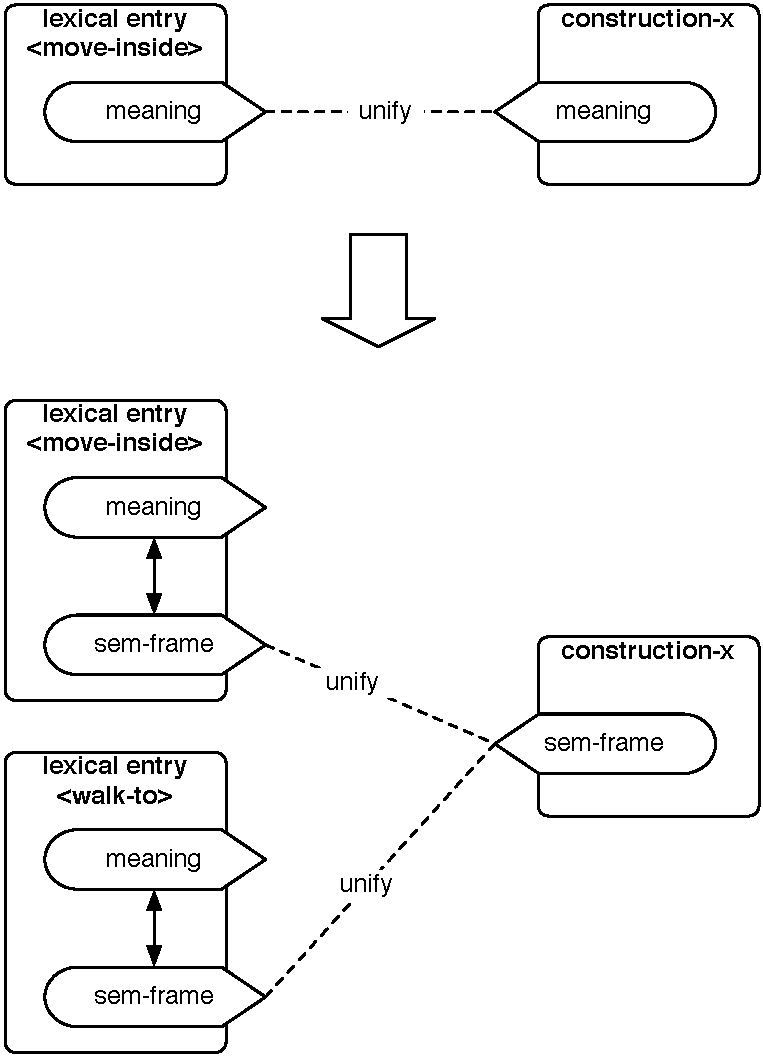
\includegraphics[width=0.7\linewidth]{Chapter3/figs/generalise}}
  \caption[Constructing generalized semantic role\is{semantic role}s]{This diagram shows how the semantics of lexical entr\is{lexical entry}ies and constructions integrate with each other. At first, constructions are verb\is{verb}-specific and unify\is{unify and merge} with the meaning of a lexical entr\is{lexical entry}y. If the agent however decides to reuse\is{reuse} this construction in a new situation, a generalized semantic role\is{semantic role} is constructed. The relevant lexical entr\is{lexical entry}ies are exten\is{extension}ded with a potential semantic frame\is{frame!semantic frame} which unifies with the semantic frame\is{frame!semantic frame} of the construction. The links between the meaning and the semantic frame\is{frame!semantic frame}s are taken care of by variable equal\is{variable equality}ities.}
   \label{f:generalise}
\end{figure}

The changes to the inventory are schematized in Figure \ref{f:generalise} and can be summarized as follows: the specific meaning in the semantic pole of the construction is removed and replaced by a semantic frame\is{frame!semantic frame} which contains the generalized semantic role\is{semantic role}. This semantic role\is{semantic role} shares the same variable as the referent of the other argument unit which was already present in the construction. The two lexical entr\is{lexical entry}ies which have to be compatible with the new construction ({\em move-inside} and {\em walk-to}) are exten\is{extension}ded with a semantic frame\is{frame!semantic frame} as well. As explained in Chapter \ref{c:ar}, this is not a frame in the traditional sense but rather a list of the potential valent\is{valency!potential valents}s of the verb\is{verb}. Since that Chapter also gives a full trace of parsing and production, I will not repeat the same operation here.


\subsubsection{Learning}
 The hearer learns the marker\is{case!case marking} by following the same strategy as before. If he didn't know the marker\is{case!case marking} yet, he will create a new verb\is{verb}-specific construction\is{construction!verb-specific construction} if the context is clear enough. If he already knew the marker\is{case!case marking}, he will get into trouble during parsing because its present use does not correspond to its previous function. The hearer will ignore the problem for the time being and parse the utterance as good as possible. Using the parsed meaning, inferred variable equal\is{variable equality}ities and re-entrance\is{re-entrance}, the agent can then (possibly) retrieve the analog\is{analogy}y introduced by the speaker. If the hearer cannot retrieve any analog\is{analogy}y, he will nevertheless accept it as imposed by the speaker.

The agents in this experiment can thus be characterized as (incremental) instan-ce-based\is{exemplar-based models} learners (and innovat\is{innovation}ors) \citep[Chapter 8]{mitchell97machine}: the agents are `lazy' learner\is{lazy learner}s in the sense that they postpone generalization until new instances have to be classified as opposed to `eager' learner\is{eager learner}s that try to make abstraction\is{abstraction}s over the data immediately. Each innovat\is{innovation}ion or novel classification is not based on abstract rules but by examining its relation to previously stored instances.  This kind of learning (and innovat\is{innovation}ion) fits usage-based model\is{usage-based model}s of language which presuppose {\em ``a bottom-up, maximalist, redundant approach in which patterns (schemas, generalizations) and instantiations are supposed to coexist, and the former are acquired from the latter''} \citep[20]{daelemans05memory}.


\subsubsection{Consolidation\is{consolidation}}
 The original two-agent simulations did not need to care about alignment strateg\is{alignment strategy}ies or consolidation\is{consolidation} too much since the two agents always share the same communicative history. So the replicating experiment should pose no problems in both the alignment of case marker\is{case!case marking}s and the alignment of the internal structure of semantic role\is{semantic role}s. The same prediction cannot be made for multi-agent simulations in which alignment strateg\is{alignment strategy}ies are needed for convergence. Three additional set-ups have therefore been implemented: one which uses the same mechanism for updating the confidence\is{confidence} scores of linguistic items as in baseline experiment 2 (set-up 3b), one in which a more fine-grained scoring mechanism has been implemented (set-up 3c), and finally one in which (token) frequency\is{frequency} decides on the speaker's behaviour (set-up 3d). In this section I will not go into the reasons for experimenting with these different set-ups: they have been inspired by the experimental results and are therefore discussed later on. Instead, I will restrict myself to explaining the two new consolidation\is{consolidation} strategies. The four different set-ups (and their effects on the results) are summarized in Table \ref{t:consolidation-comparison}.


{\bfseries {\em Set-up 3c. }}The more fine-grained scoring mechanism implemented in set-up 3c is based on the idea that linguistic items are not `good or bad', but that they may be more suitable in some particular contexts and less suitable in others. A single confidence\is{confidence} score for every linguistic item cannot go beyond its black-or-white updating scheme and thus cannot handle a more nuanced way of processing. Instead, agents need more clever self-assess\is{self-assessment}ment criteria: next to communicative success\is{communicative success}, they can use {\bfseries co-occur\is{co-occurrence}rences} of linguistic items as a source for aligning their inventories. 

Co-occurring items are locally observable to the agents since they form one chain in the reaction network\is{reaction network} during processing. The general idea is reminiscient of Hebbian learning\is{Hebbian learning} (`what fires together, wires together'): a link is kept between co-occur\is{co-occurrence}ring items and a confidence\is{confidence} score is kept for this link based on the successful co-occur\is{co-occurrence}rence of both items. Suppose that the agent has the case marker\is{case!case marking} {\em -ma} (see the example earlier in this section) which may cover either the participant role\is{participant role} walk-to-2 or the role move-inside-1. The idea is now that the agents keep a link between co-occur\is{co-occurrence}ring linguistic items, so the agent would now have a link between construction-x one the one hand and the two lexical entr\is{lexical entry}ies {\em walk-to} and {\em move-inside} on the other. Instead of positing a score on the complete construction, each co-occur\is{co-occurrence}rence link has its own confidence\is{confidence} score: 

\ea
\begin{align*}
\text{<Construction-x>} & \leftarrow  
\begin{array}{ll} 
0.5 \rightarrow & \text{<move-inside> (for move-inside-1) }\\
0.5 \rightarrow & \text{<walk-to> (for walk-to-2)}
\end{array}
\end{align*}
\z

Suppose that the speaker also has the marker\is{case!case marking} {\em -bo} which can be used for marking `move-1' and `move-inside-2':

\ea
\begin{align*}
\text{<Construction-y>} & \leftarrow  
\begin{array}{ll} 
0.5 \rightarrow & \text{<move-inside> (for move-inside-1)} \\
0.5 \rightarrow & \text{<move> (for move-1)}
\end{array}
\end{align*}
\z

If the agent then observes the co-occur\is{co-occurrence}rence of construction-x and {\em move-inside} (i.e. the agent analyzes an utterance in which {\em -ma} was used for marking move-inside-1), the score of the link is increased with 0.1 and the score of competing links (here the link between {\em move-inside} and construction-y) is decreased by 0.1. The other confidence\is{confidence} scores based on co-occur\is{co-occurrence}rence remain untouched:

\ea
\begin{align*}
\text{<Construction-x>} & \leftarrow  
\begin{array}{ll} 
0.6 \rightarrow & \text{<move-inside> (for move-inside-1) }\\
0.5 \rightarrow & \text{<walk-to> (for walk-to-2)}
\end{array}
\\
\text{<Construction-y>} & \leftarrow  
\begin{array}{ll} 
0.4 \rightarrow & \text{<move-inside> (for move-inside-1)} \\
0.5 \rightarrow & \text{<move> (for move-1)}
\end{array}
\end{align*}
\z

Note that this score is not the actual co-occur\is{co-occurrence}rence frequency\is{frequency}, but a confidence\is{confidence} score between 0 and 1 which only indirectly reflects co-occur\is{co-occurrence}rence and which is updated based on communicative success\is{communicative success}.


{\bfseries {\em Set-up 3d. }} The fourth set-up in baseline experiment 3 removes the explicit lateral inhibition\is{lateral inhibition} consolidation\is{consolidation} of the previous set-ups and replaces it with a combination of {\bfseries token frequency\is{token frequency}\is{frequency} and memory decay\is{memory decay}}. Frequency is implemented as a simple counter which can be updated after each interaction. This set-up has the following features:

\begin{itemize}
\item During production, the speaker will use the linguistic items which have the highest frequency\is{frequency} score;
\item After each {\em successful} interaction, the hearer will increase the counter of all the constructions that were applied during parsing by one;
\item When an agent has engaged in 50 interactions, all the frequency\is{frequency} scores are decreased by one (= memory decay\is{memory decay}).
\end{itemize}

This kind of (token) frequency\is{frequency} favours more general constructions: the larger the type frequency\is{type frequency}\is{frequency} of a certain class or category, the more chances it has to increase its token frequency\is{token frequency}\is{frequency}. The memory decay\is{memory decay} implemented here is unaffected by population\is{speech population} size since it is based on each agent's individual history. It is, however, sensitive to inventory size and frequency\is{frequency}: linguistic items can only survive if they occur at least once before the next decay is performed. In the present set-up, each participant role\is{participant role} occurs one time out of thirty interactions on average.

\subsection{Results and discussion of set-up 3a}

\begin{figure}[ht]
\centerline{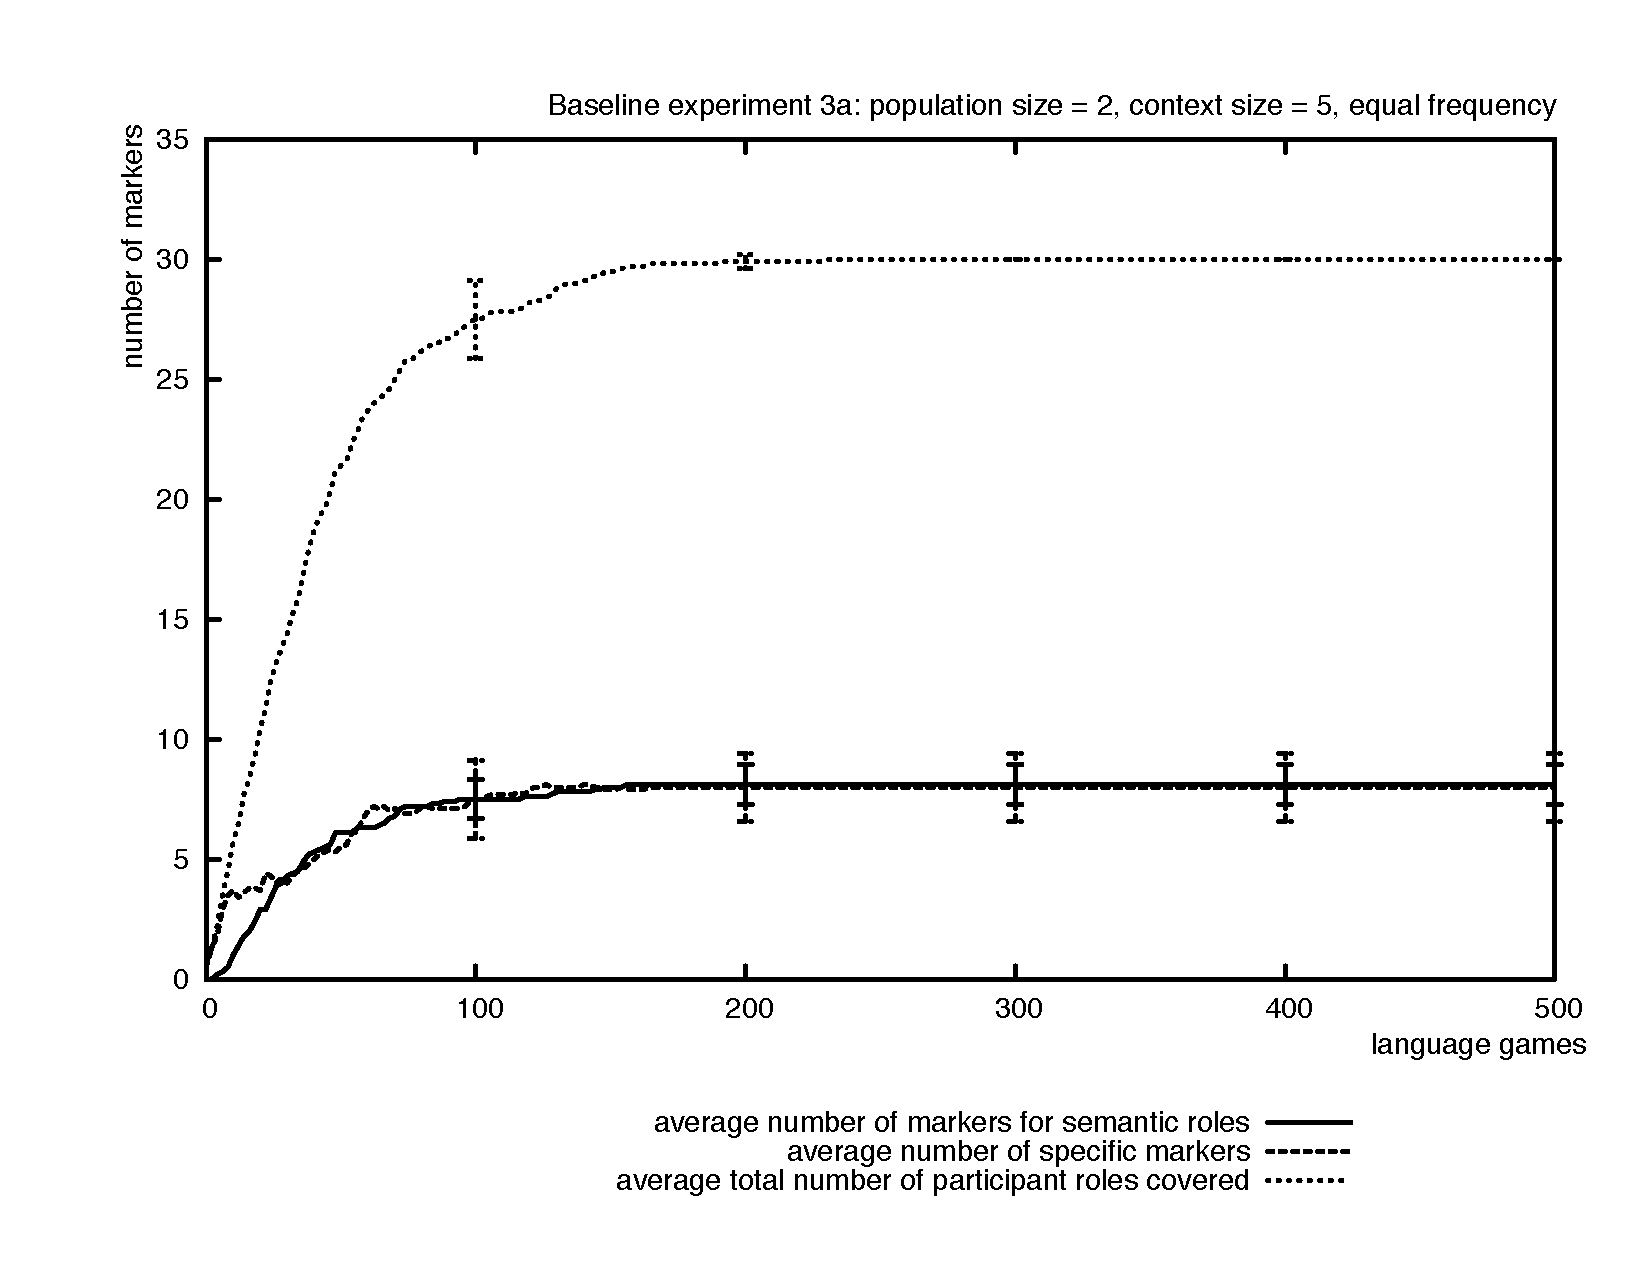
\includegraphics[width=0.9\textwidth]{Chapter3/figs/graph-base3-size3a}}
  \caption[Baseline experiment 3a: number of markers]{In the two-agent simulations, the agents have no problems aligning their inventories since there is no variation\is{variation} in the population\is{speech population}. In ten series of 500 language game\is{language game}s, the agents came up with an average of 6-8 marker\is{case!case marking}s for semantic role\is{semantic role}s and an average of 6-9 marker\is{case!case marking}s for specific participant role\is{participant role}s. The semantic role\is{semantic role}s gather together up to 24 participant role\is{participant role}s out of 30.}
   \label{f:base3-size3a}
\end{figure}

\subsubsection{Results}
 The replicating experiment featuring a population\is{speech population} of two agents confirms the results obtained by \citet{steels02simulating, steels04constructivist}. The agents succeed in reusing\is{reuse} existing marker\is{case!case marking}s and generalizing them to semantic role\is{semantic role}s as is shown in Figure \ref{f:base3-size3a} . During ten series of 500 language game\is{language game}s, the agents constructed on average 6 to 8 marker\is{case!case marking}s which could be used for covering at least two participant role\is{participant role}s. In total, up to 24 participant role\is{participant role}s out of 30 were grouped together in more general roles. In each simulation, also 6 to 9 marker\is{case!case marking}s survived which cover specific participant role\is{participant role}s.

A closer examination of the semantic role\is{semantic role}s learns us that they tend to be small generalizations mostly covering two participant role\is{participant role}s. Some roles exceptionally gather four or even six participant role\is{participant role}s. Here are some example sentences from one of the simulations and their glosses:

\ea
\gll jack -cui walk-to jill -ge \\
jack sem-role-6 walk-to  jill sem-role-26 \\
\glt `Jack walks to Jill.' \\

\item
\gll touch jill -cui house -shae \\
touch jill sem-role-6 house-1 sem-role-29 \\
\glt `Jill touches house-1.' \\

\item
\gll house -lu move-inside boy -cui \\
house-1 sem-role-10 move-inside boy sem-role-6 \\
\glt `The boy moves inside house-1.' \\

\z

In the same simulation, the following marker\is{case!case marking}s and their corresponding participant role\is{participant role}s were constructed (ranging from 7 specific marker\is{case!case marking}s to 8 more general ones):

\begin{itemize}
\item -vuh: cause-move-on-1
\item -yaem: cause-move-on-2
\item -jibui: cause-move-on-3
\item -shuip: give-3
\item -vot: take-3
\item -me: visible-1
\item -naez: move-outside-2
\item -zo: fall-1, approach-1
\item -tui: fall-2, approach-2
\item -shae: touch-2, give-2
\item -fe: distance-decreasing-1, grasp-1
\item -lu: move-inside-2, distance-decreasing-2
\item -we: move-1, give-1, take-1
\item -cui: walk-to-1, object-1, grasp-2, hide-2
\item -ge: touch-1, move-inside-1, move-outside-1, hide-1, walk-to-2, take-2
\end{itemize}

\subsubsection{Discussion}
 The results show that the construction of generalized semantic role\is{semantic role}s allows the agents to reduce the number of marker\is{case!case marking}s by 65--70\%. However, the most important observation is that by endowing the agents with the capacity of analog\is{analogy}ical reasoning, they are capable of generalization beyond previous linguistic experience as is shown in the increasing productivity\is{productivity} of some marker\is{case!case marking}s.

In the results there is still a fairly large residue of verb\is{verb}-specific marker\is{case!case marking}s which is partly due to the analog\is{analogy}y algorithm and partly due to the fact that only two agents were involved in the simulation. First, the analog\is{analogy}y algorithm is very strict in the sense that two roles are either analog\is{analogy}ous or not: there is no in-between value that allows for some flexibility. Second, since there are no variation\is{variation}s in the population\is{speech population}, the construction of semantic role\is{semantic role}s is entirely dependent on the linguistic history of both agents: once an analog\is{analogy}y is constructed and successfully applied in communication, the agents will not try to come up with better or more general analog\is{analogy}ies later on. In other words, the solutions that the two agents come up with may not be optimal given their search space so they end up in a local maximum. A larger population\is{speech population} may give this search an additional boost.

\subsection{Results and discussion of set-up 3b}

\begin{figure}[ht]
\centerline{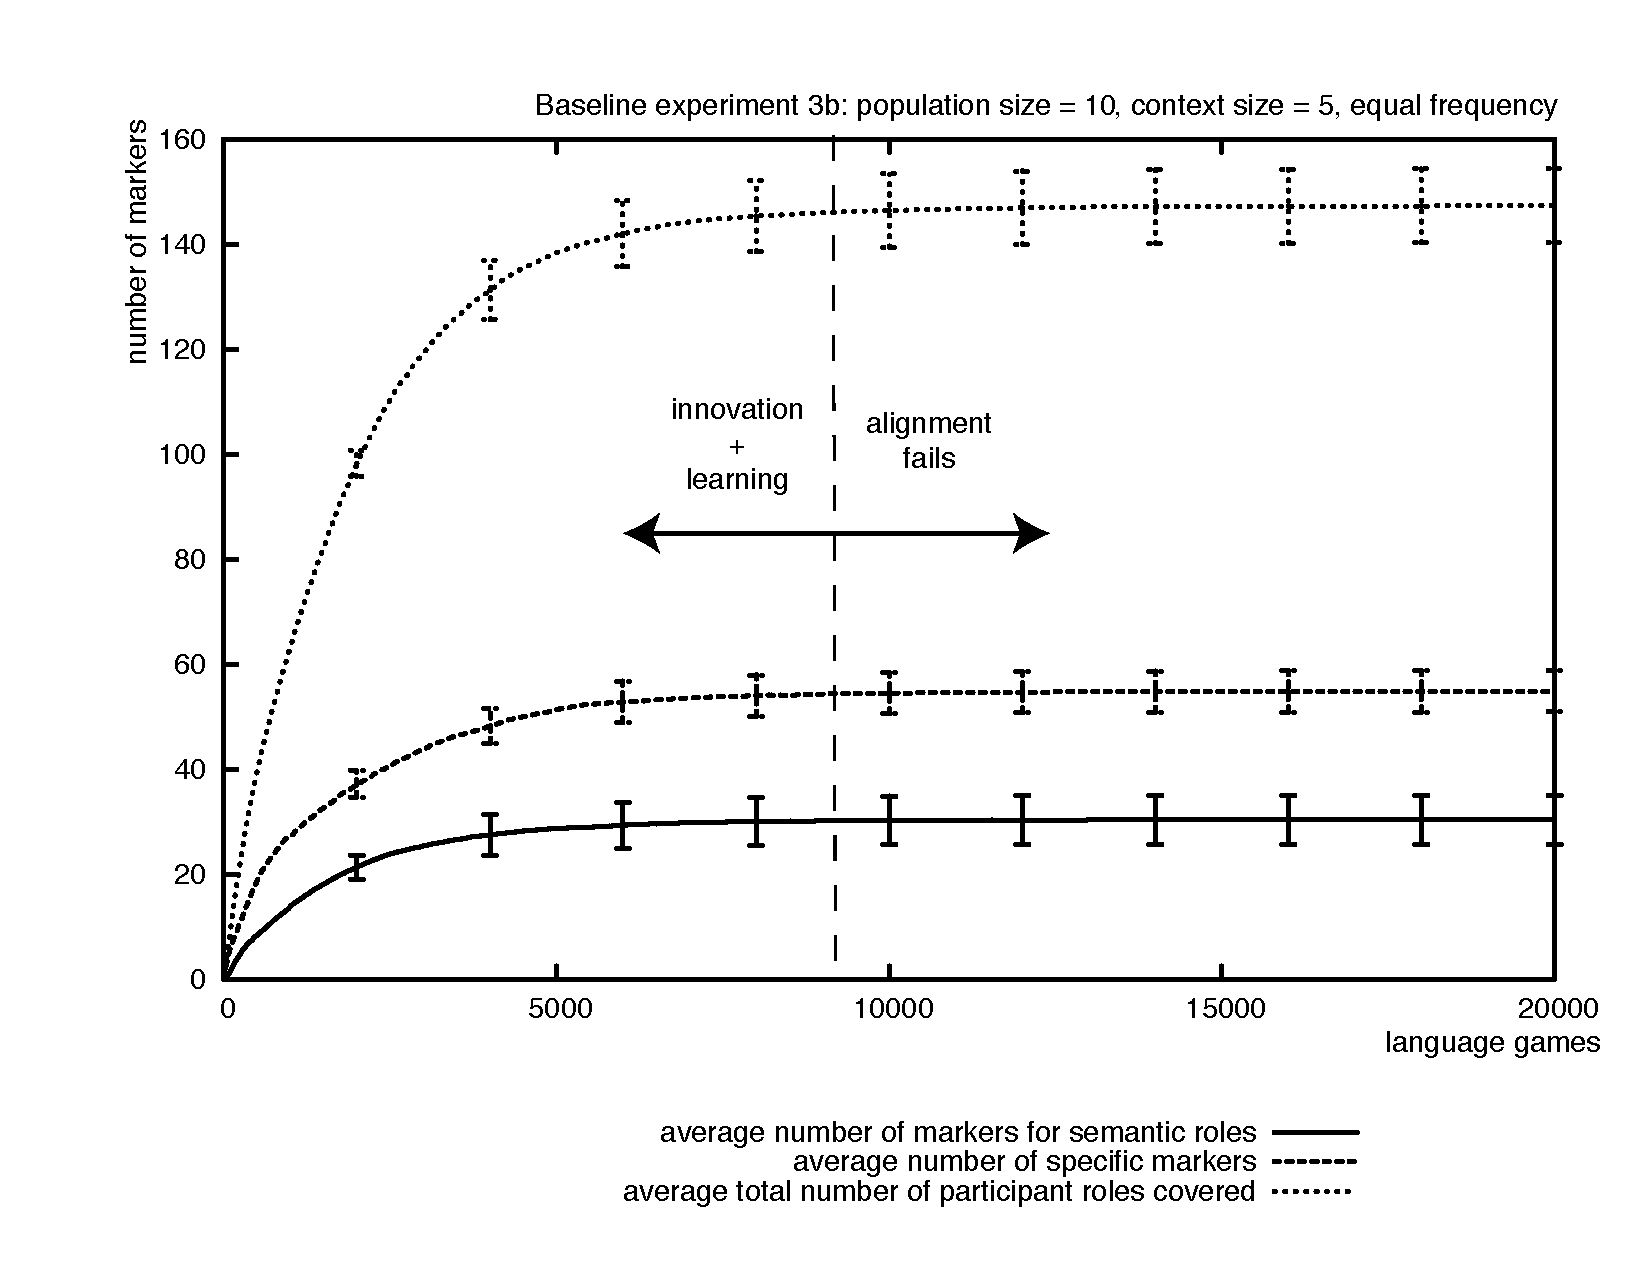
\includegraphics[width=0.9\textwidth]{Chapter3/figs/graph-base3-size3b}}
  \caption[Baseline experiment 3b: number of markers]{When scaling the experiments up to multi-agent simulations, the traditional alignment strateg\is{alignment strategy}ies used in prior experiments on lexicon\is{lexicon} formation\is{formation} are not sufficient for the population\is{speech population} to reach convergence. For thirty participant role\is{participant role}s, the agents have to remember 140 variation\is{variation}s to communicate successfully, which is an average of 4,7 possible ways for marking each participant role\is{participant role}.}
   \label{f:base3-size3b}
\end{figure}

\subsubsection{Results}
 In set-up 3b the population\is{speech population} size is increased to 10 agents so there will be more variation\is{variation} among the agents. This is indeed confirmed in Figure \ref{f:base3-size3b} which shows that there are a total of 140 variation\is{variation}s floating in the population\is{speech population} for marking 30 participant role\is{participant role}s. This is an average of 4,7 possible ways for marking each participant role\is{participant role}. This number of possibilities does not drop to 30, which is a first indication that the agents do not converge on a shared set of grammatical marker\is{case!case marking}s. As for the nature of the marker\is{case!case marking}s, the results indicate that there are about 20 marker\is{case!case marking}s that can be used for covering at least two participant role\is{participant role}s whereas there are about 50 specific participant role\is{participant role} marker\is{case!case marking}s as well. The average inventory size of the agents is thus far from optimal.

Figure \ref{f:base3-effort3b} confirms that the agents do not reach convergence: the meaning-form coherence indicates the degree to which the agents prefer the same case marker\is{case!case marking} for a particular participant role\is{participant role}. As the graph shows, coherence only reaches 40\% which means that the agents use a different marker\is{case!case marking} for the same participant role\is{participant role} in more than half of the language game\is{language game}s. Yet, as the graph also shows, the agents are capable of reaching 100\% communicative success\is{communicative success}  and reducing the cognitive effort\is{cognitive effort} to zero.
\begin{figure}[t]
\centerline{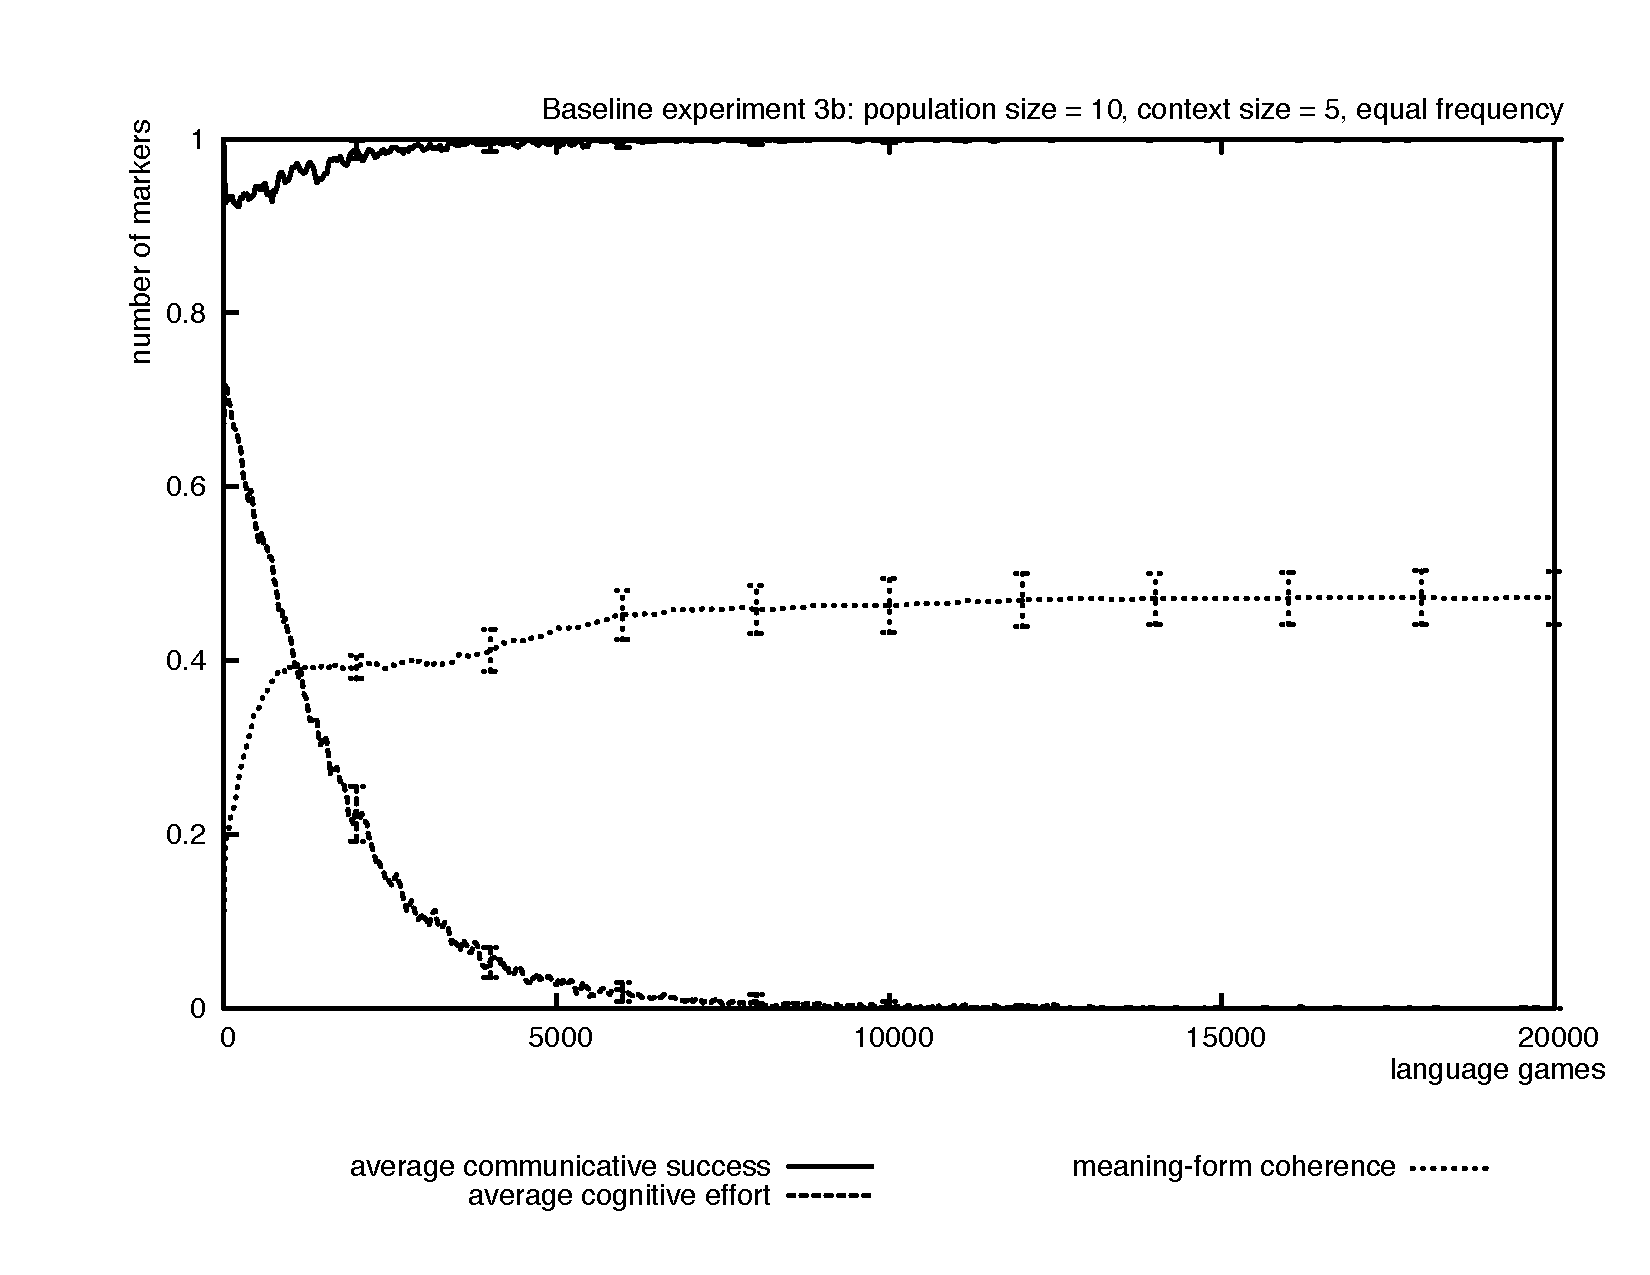
\includegraphics[width=\textwidth]{Chapter3/figs/graph-base3-effort3b}}
  \caption[Baseline experiment 3b: success, effort and coherence]{This graph shows that the agents reach 100\% communicative success\is{communicative success} and reduce the cognitive effort\is{cognitive effort} needed for interpretation. However, the meaning-form coherence only reaches about 40\% which indicates that the agents did not converge on a shared set of marker\is{case!case marking}s but keep using divergent preferences in more than half of the language game\is{language game}s.}
   \label{f:base3-effort3b}
\end{figure}


\subsubsection{Discussion}
 The results of baseline experiment 3b seem to be contradictory at first sight: even though the agents do not agree an a shared preferred set of marker\is{case!case marking}s, they nevertheless reach communicative success\is{communicative success}. This is possible because success in communication does not require meaning-form coherence: if the agents learn all the variation\is{variation}s floating around in the population\is{speech population}, they can still parse all utterances correctly. This happens indeed in this experiment.

The lack of convergence on a preferred set of marker\is{case!case marking}s clearly indicates that the proposed alignment strateg\is{alignment strategy}y is insufficient. The reason is that the alignment strateg\is{alignment strategy}y in which each item has its own single confidence\is{confidence} score is best suited for simulations in which there is always a {\em one-to-one} mapping between form and meaning (as was the case in baseline experiment 2). However, when marker\is{case!case marking}s get generalized to cover more than one participant role\is{participant role}, they become polysemous {\em one-to-more} mappings.

I will go through an example to explain why the single confidence\is{confidence} score cannot be sufficient for polysemous form-meaning mappings. Suppose that an agent knows three marker\is{case!case marking}s: {\em -ma}, {\em -bo} and {\em -li} and that the first two are generalized to cover two roles each whereas {\em -li} is still a verb\is{verb}-specific marker\is{case!case marking}. For convenience's sake, I will not include all the linguistic items involved but treat the marker\is{case!case marking}s as if they were lexical items:

\begin{align*}
\begin{array}{ll} 
\text{<move-inside-1>} & \leftarrow \\
\text{<walk-to-2>} & \leftarrow
\end{array}
& \text{(0.5)}\rightarrow \text{-ma}
\end{align*}

\begin{align*}
\begin{array}{ll} 
\text{<move-inside-1>} & \leftarrow \\
\text{<move-1>} & \leftarrow
\end{array}
& \text{(0.5)}\rightarrow \text{-bo}
\end{align*}

\begin{align*}
\begin{array}{ll}
\text{<move-1>}\hspace{1,05cm} & \leftarrow
\end{array}
& \text{(0.5)}\rightarrow \text{-li}
\end{align*}

Suppose now that the agent observes the utterance {\em boy -ma move-inside} in which the marker\is{case!case marking} {\em -ma} was successfully used for marking `move-inside-1'. The score for {\em -ma} is thus increased and the score for its competit\is{competition}or {\em -bo} is decreased. The consequences for {\em -bo} are far-reaching, because it is now not only less successful than {\em -ma} for covering `move-inside-1', but also than {\em -li} for marking `move-1':

\begin{align*}
\begin{array}{ll} 
\text{<move-inside-1>} & \leftarrow \\
\text{<walk-to-2>} & \leftarrow
\end{array}
& \text{(0.6)}\rightarrow \text{-ma}
\end{align*}

\begin{align*}
\begin{array}{ll} 
\text{<move-inside-1>} & \leftarrow \\
\text{<move-1>} & \leftarrow
\end{array}
& \text{(0.4)}\rightarrow \text{-bo}
\end{align*}

\begin{align*}
\begin{array}{ll}
\text{<move-1>}\hspace{1,05cm} & \leftarrow
\end{array}
& \text{(0.5)}\rightarrow \text{-li}
\end{align*}

In another game, the same damage can be done for the marker\is{case!case marking} {\em -ma} so {\em -bo} can recover from its score decrease. Generalization thus tends to be harmful for the marker\is{case!case marking}s if only one score is used: the more general a role marker\is{case!case marking} gets, the more competit\is{competition}ors it has and thus the more chances that its score will be decreased. Specific marker\is{case!case marking}s can escape punishment through lateral inhibition\is{lateral inhibition} much more easily. On the other hand, if it has competing marker\is{case!case marking}s which are generalized, they can get punished too even if a different participant role\is{participant role} was involved. Suppose that {\em -bo} was observed for marking `move-inside-1' this time, then not only {\em -ma} is seen as a competit\is{competition}or, but also {\em -li} because it overlaps with {\em -bo} for marking `move-1'.

There is thus a constant push-and-pull effect in which marker\is{case!case marking}s may get cornered by others but then all of a sudden get more successful again. This is the reason why the agents can never converge on a preferred set: the single confidence\is{confidence} score does not allow marker\is{case!case marking}s to be successful in one particular context but unsuccessful in another.

\subsection{Results and discussion of set-up 3c}

\begin{figure}[t]
\centerline{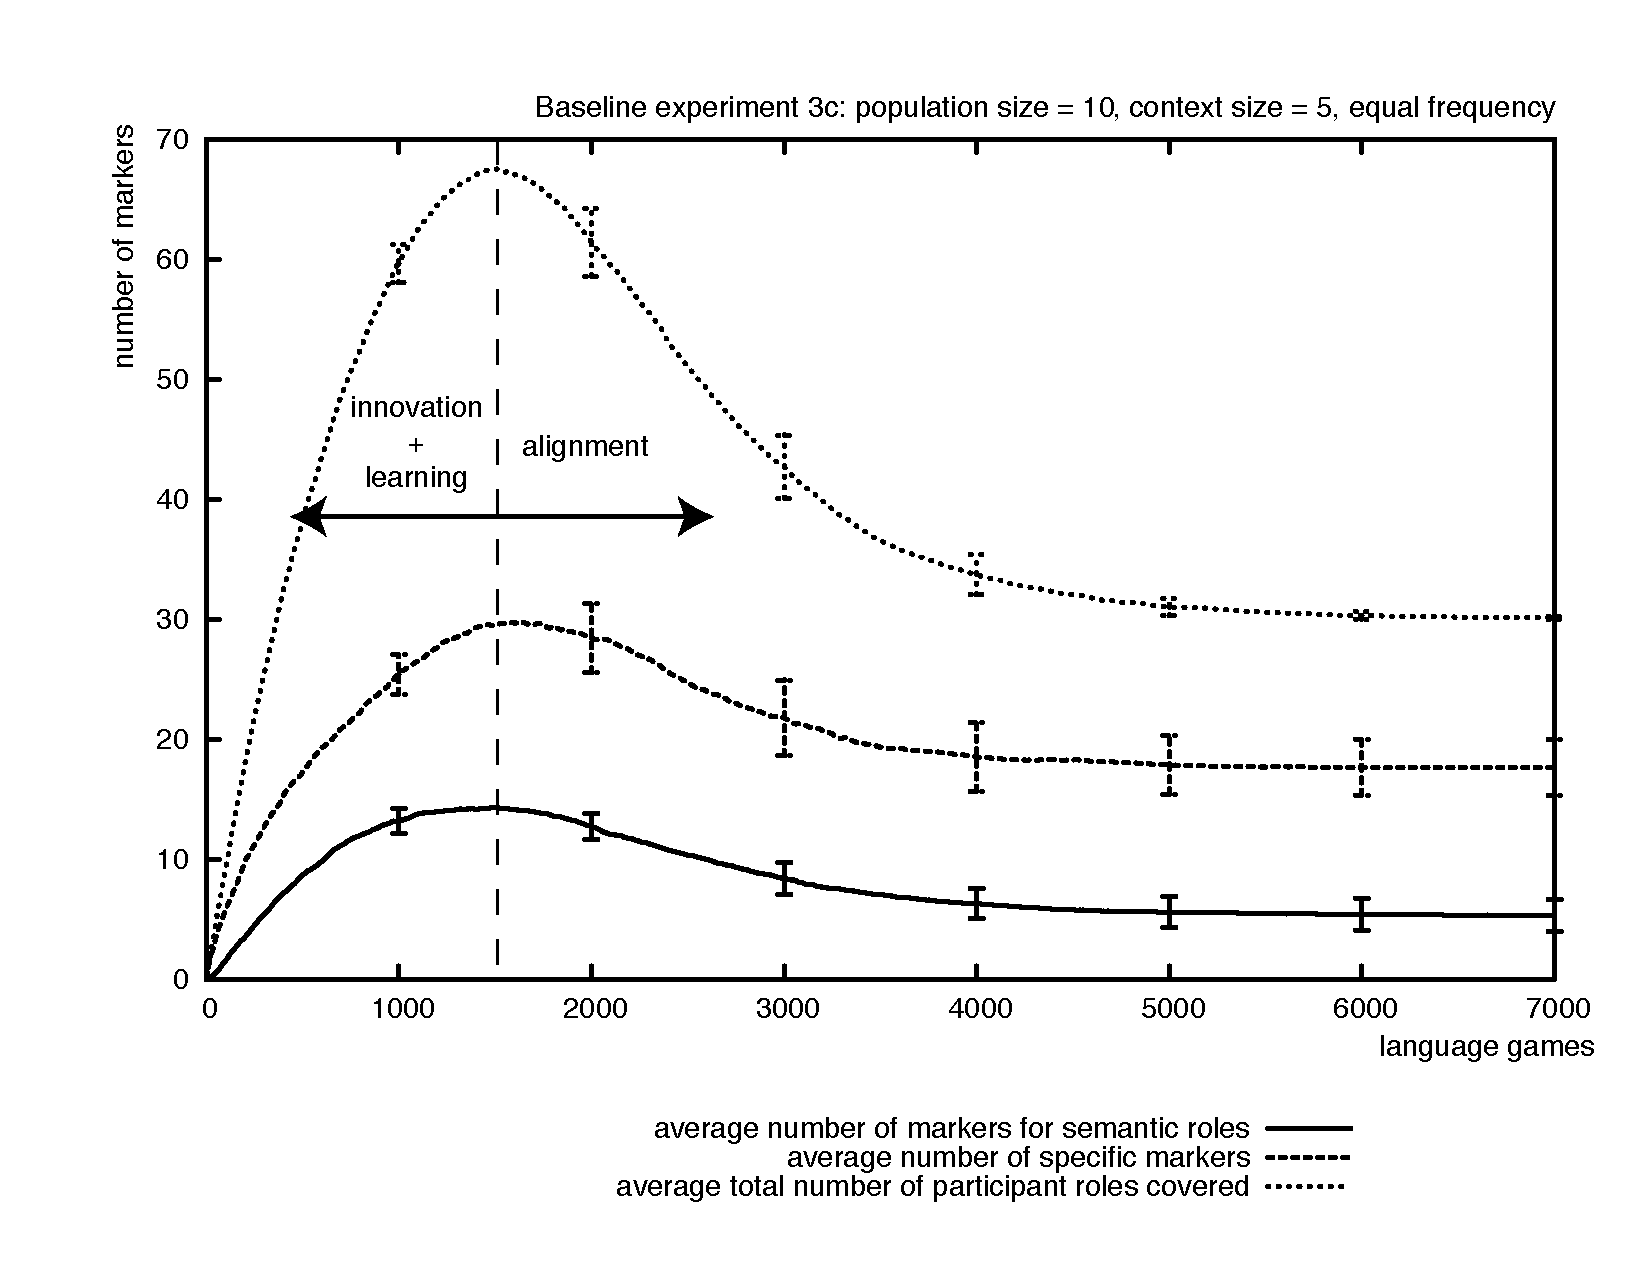
\includegraphics[width=\textwidth]{Chapter3/figs/graph-base3-size3c}}
  \caption[Baseline experiment 3c: number of markers]{The more fine-grained alignment strateg\is{alignment strategy}y allows the agents to converge on one possible marking for each of the thirty participant role\is{participant role}s. There are 5 semantic role\is{semantic role}s on average which each cover about two participant role\is{participant role}s. The remaining 20 roles are covered by specific marker\is{case!case marking}s.}
   \label{f:base3-size3c}
\end{figure}

\begin{figure}[ht]
\centerline{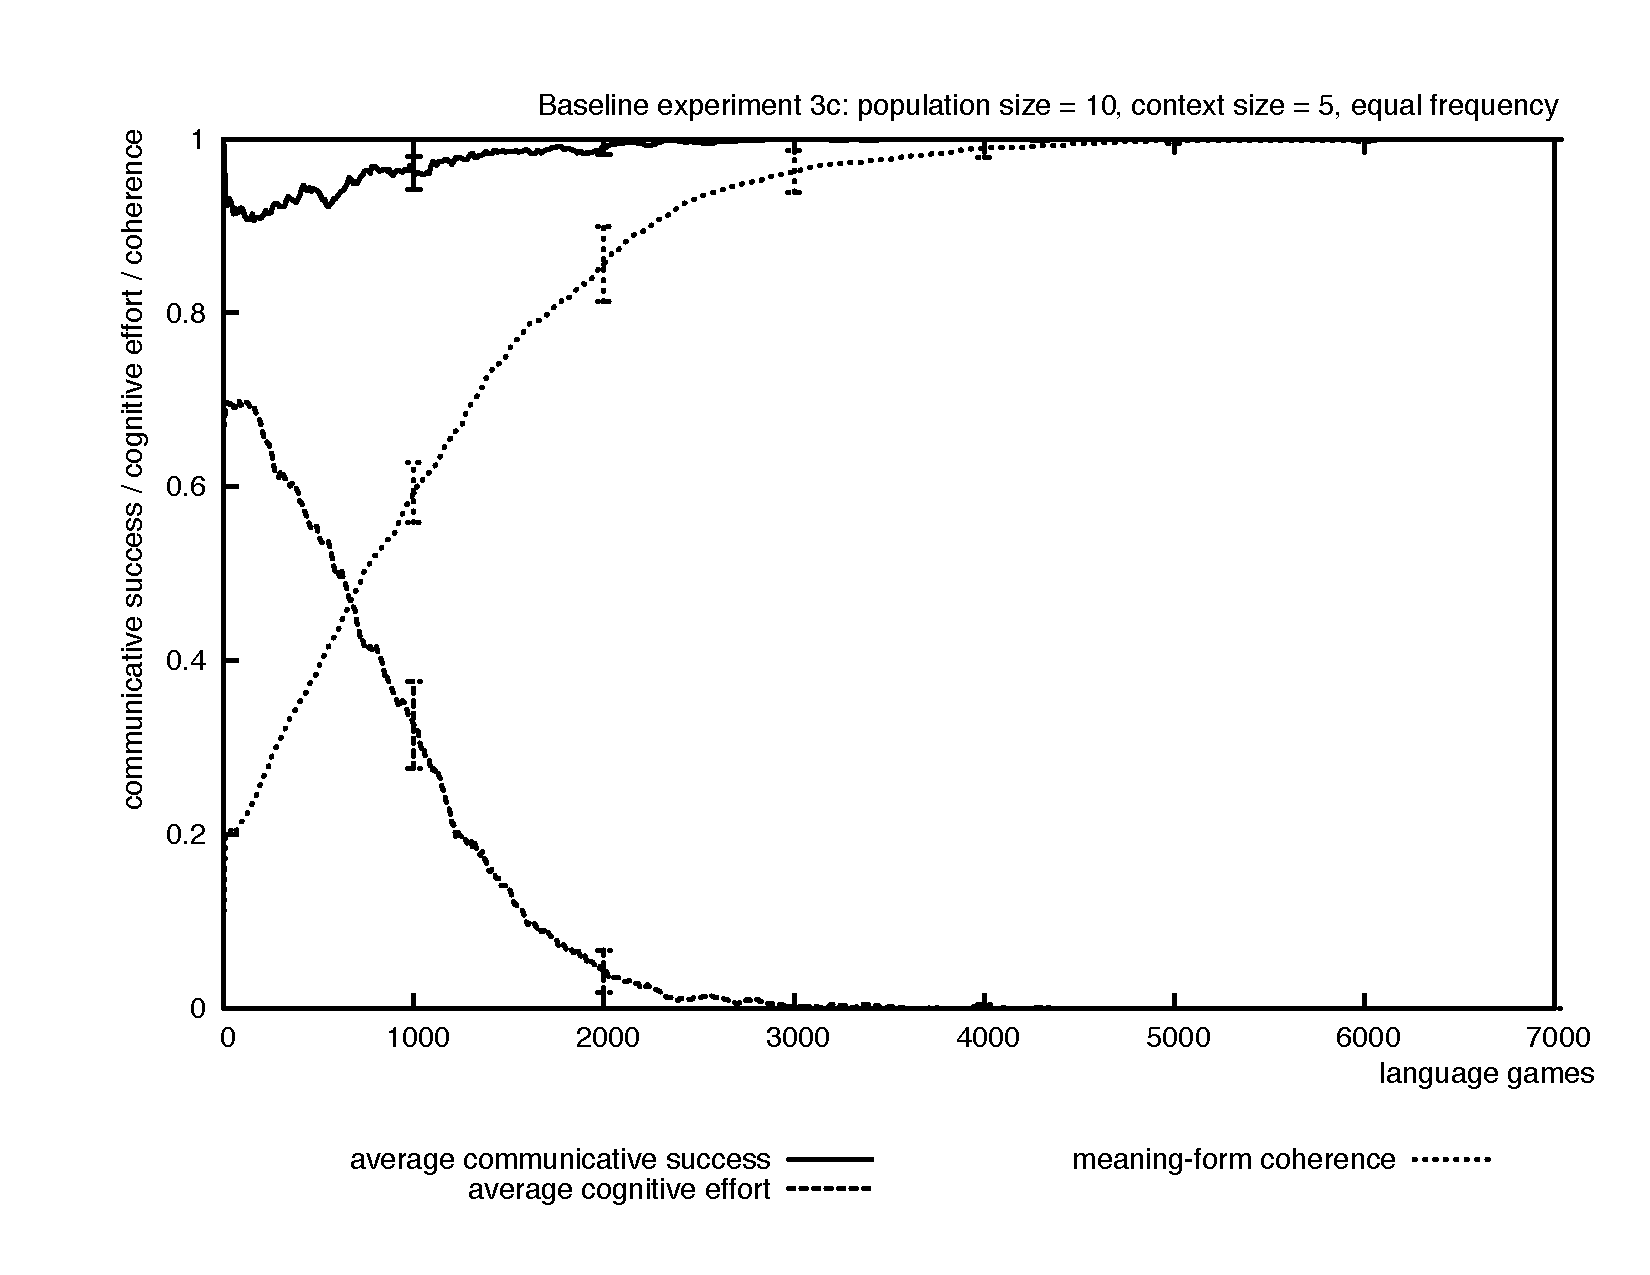
\includegraphics[width=\textwidth]{Chapter3/figs/graph-base3-effort3c}}
  \caption[Baseline experiment 3c: success, effort and coherence]{Using the more fine-grained alignment strateg\is{alignment strategy}y, the agents not only succeed in reaching communicative success\is{communicative success} and reducing cognitive effort\is{cognitive effort}, they also converge on a shared set of meaning-form convention\is{convention}s.}
   \label{f:base3-effort3c}
\end{figure}

\subsubsection{Results}
 The results of baseline experiment 3c indicate that the alignment strateg\is{alignment strategy}y of reinforc\is{reinforcement}ement and lateral inhibition\is{lateral inhibition} can lead to convergence if it is applied in a more fine-grained way. This time, the agents not only use communicative success\is{communicative success} as a guidance but also co-occur\is{co-occurrence}rence links: instead of positing one score on the linguistic item as a whole, they now keep a link between co-occur\is{co-occurrence}ring items and assign a confidence\is{confidence} score to that link. In case of success, the score of the link is increased and only scores of competing {\em links} are decreased. In this model, a marker\is{case!case marking} disappears from the linguistic inventor\is{linguistic inventory}y once it has no links to other linguistic items anymore with a confidencescore higher than zero.

Figure \ref{f:base3-size3c} shows that the number of variation\is{variation}s peaks at 70 possible markings for 30 participant role\is{participant role}s. This means that the agents only have to deal with an average of 2,3 competing marker\is{case!case marking}s for each participant role\is{participant role}. Innovation and adoption of marker\is{case!case marking}s stops at about 1.500 language game\is{language game}s after which the agents rapidly converge on a shared set of marker\is{case!case marking}s. The graph also shows that the agents converge on a set of 5 generalized semantic role\is{semantic role} marker\is{case!case marking}s and about 20 verb\is{verb}-specific marker\is{case!case marking}s. This means that the verb\is{verb}-specific marker\is{case!case marking}s managed to win the competit\is{competition}ion more often than generalized marker\is{case!case marking}s and that semantic role\is{semantic role}s on average only cover two participant role\is{participant role}s.

Figure \ref{f:base3-effort3c} shows that fine-grained alignment allows the agents to converge on a shared set of preferences: meaning-form coherence reaches 100\% after 5.000 language game\is{language game}s which corresponds to the moment where the agents have pruned all the variation\is{variation}s down to 30 in Figure \ref{f:base3-size3c}. The agents also reach communicative success\is{communicative success} and manage to reduce the cognitive effort\is{cognitive effort} needed during parsing.


\subsubsection{Discussion}
 The results show that the fine-grained scoring mechanism suffices to solve the problem of convergence among the agents. However, the gain in inventory optimization is minimal: the agents end up with an average of 25 marker\is{case!case marking}s for 30 participant role\is{participant role}s. Also the benefits of generalization are on the low side with an average of two participant role\is{participant role}s covered by a semantic role\is{semantic role}.

By solving the problem of the single confidence\is{confidence} scores, the fine-grained scoring mechanism created a new one: since only competing links are taken into account during consolidation\is{consolidation}, the influence of the frequency\is{frequency} of the entire category is neglected. This means that a verb\is{verb}-specific marker\is{case!case marking} has the same chances of surviving the competit\is{competition}ion as generalized semantic role\is{semantic role} marker\is{case!case marking}s do, even though the latter ones are as a whole more frequent and productive. If a semantic role\is{semantic role} loses the competit\is{competition}ion from a specific marker\is{case!case marking}, its type frequency\is{type frequency}\is{frequency} is reduced and hence its productivity\is{productivity}.

To overcome this problem, the agents need another alignment strateg\is{alignment strategy}y which both recognizes the impact of generalized roles and is capable of dealing with the context-sensitive nature of polysemous marker\is{case!case marking}s. Experiment 3d implements such a strategy.

\subsection{Results and discussion of set-up 3d}

\begin{figure}[ht]
\centerline{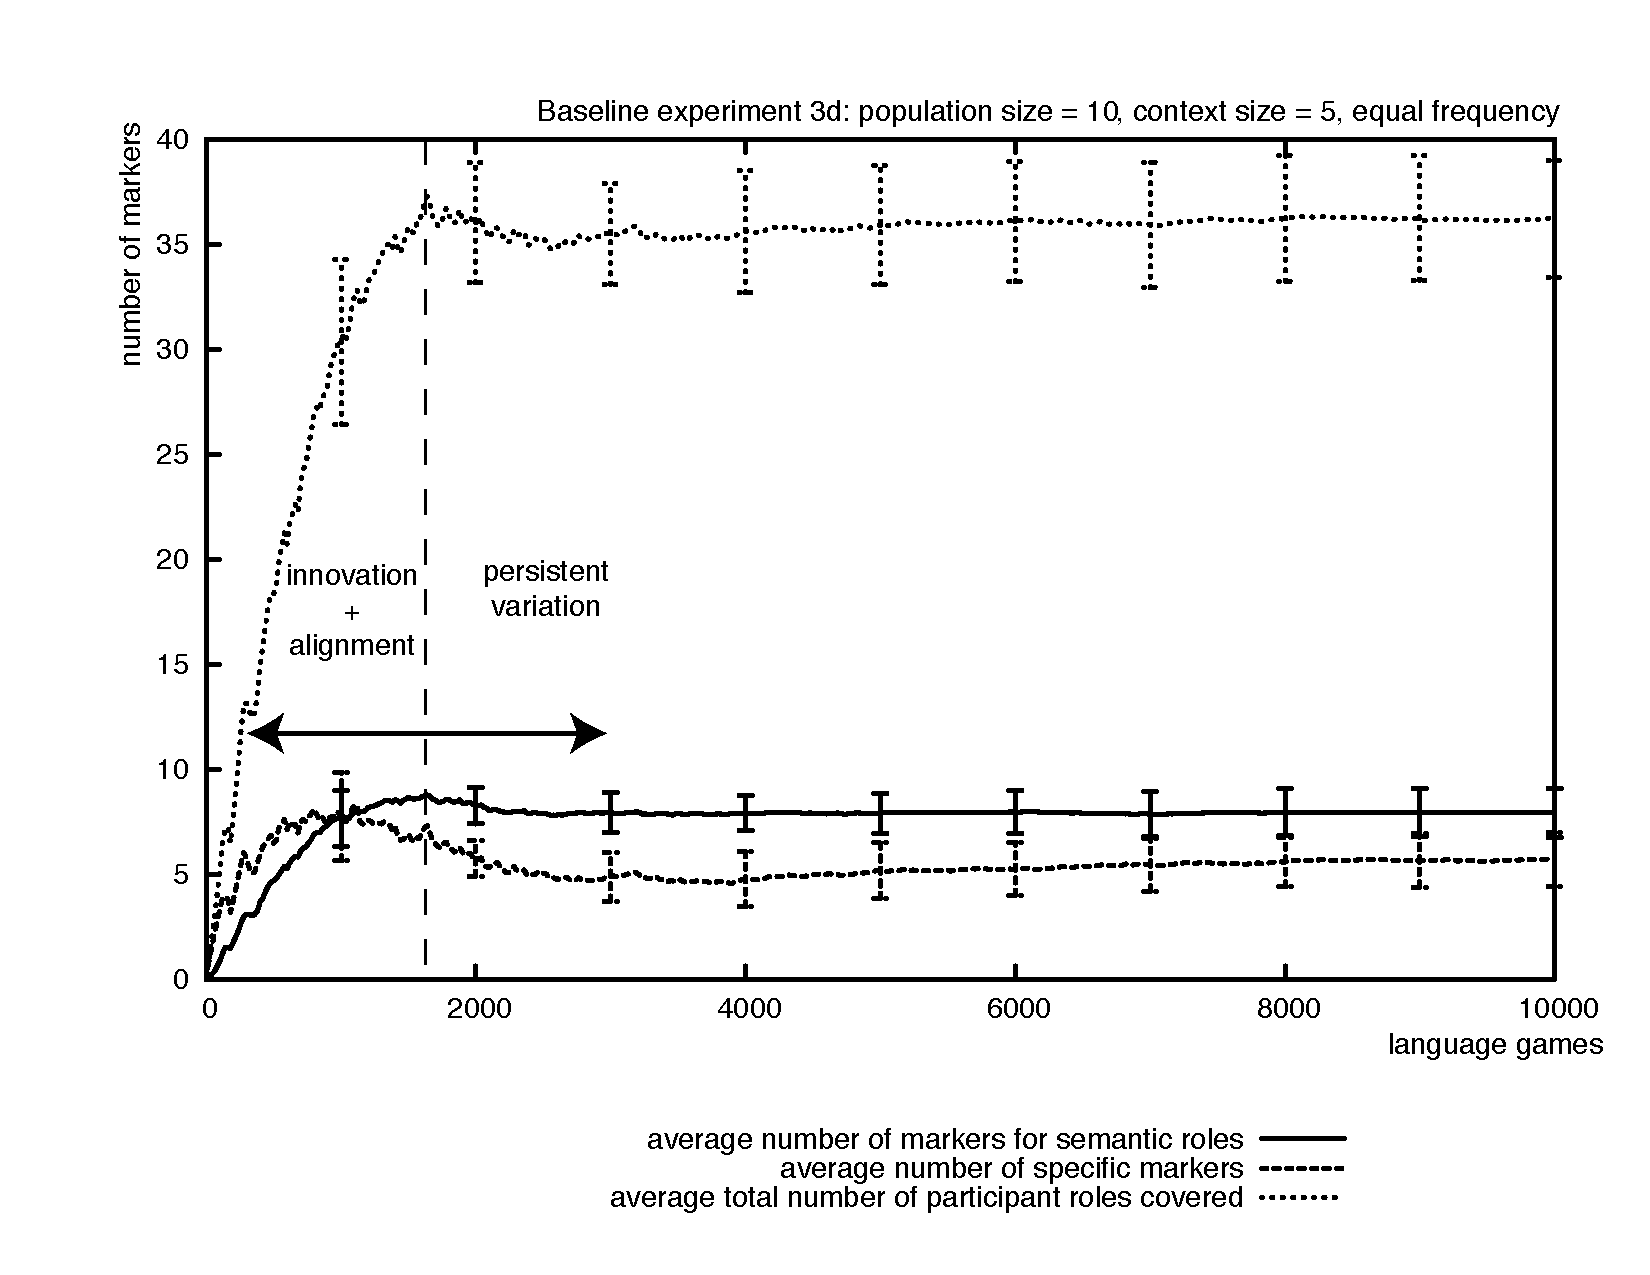
\includegraphics[width=\textwidth]{Chapter3/figs/graph-base3-success3d}}
  \caption[Baseline experiment 3d: number of markers]{When adapting their linguistic behaviours to frequency\is{frequency}, the agents tend to use more generalized semantic role\is{semantic role} marker\is{case!case marking}s rather than specific ones. Here, about seven semantic role\is{semantic role}s cover 25 of the 30 participant role\is{participant role}s. The top line indicates that some amount of variation\is{variation} persists over time.}
   \label{f:base3-size3d}
\end{figure}

\begin{figure}[ht]
\centerline{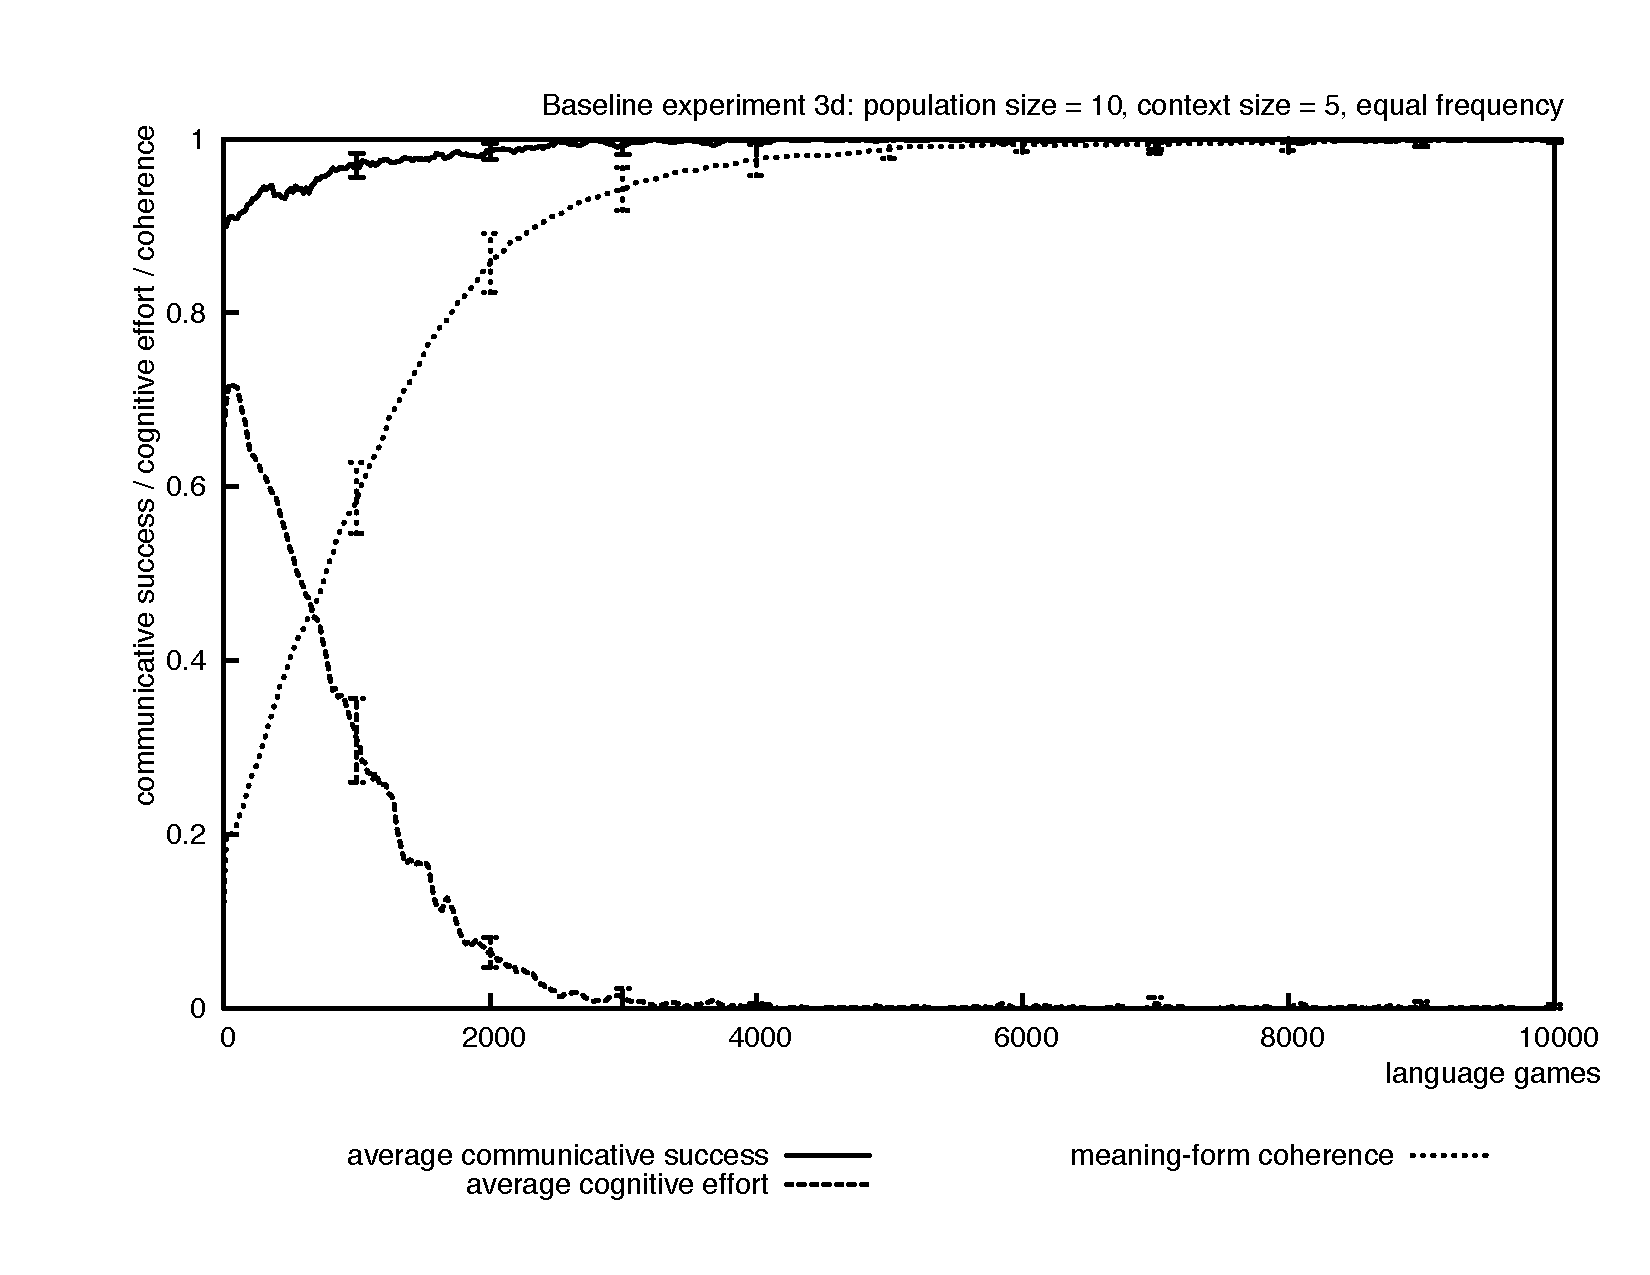
\includegraphics[width=\textwidth]{Chapter3/figs/graph-base3-effort3d}}
  \caption[Baseline experiment 3d: success, effort and coherence]{This graph shows that the agents reach communicative success\is{communicative success}, reduce the cognitive effort\is{cognitive effort} needed for interpretation and converge on a shared set of case marker\is{case!case marking}s.}
   \label{f:base3-effort3d}
\end{figure}

\subsubsection{Results}
 The final set-up in baseline experiment 3 does not use confidence\is{confidence} scores or lateral inhibition\is{lateral inhibition}. Instead, agents rely on token frequency\is{token frequency}\is{frequency} of successful interactions for producing utterances. Figure \ref{f:base3-size3d} shows that the agents spend roughly the same time as in set-up 3c innovat\is{innovation}ing and learning new marker\is{case!case marking}s. The average amount of variation\is{variation} reaches a total of 35--40 possibilities for 30 marker\is{case!case marking}s, which is an average of less than two variation\is{variation}s for each participant role\is{participant role}. The innovat\is{innovation}ion rate is in fact as high as in the previous set-up, but many innovat\is{innovation}ions are excluded very early on by memory decay\is{memory decay}. Innovations that do survive the memory decay\is{memory decay} during the first 2.000 interactions are quite frequent so they persist in memory for a very long time afterwards. Getting rid of them is therefore very slow and may take thousands of additional language game\is{language game}s before they are `forgotten' or in some cases they persist over time. A closer look at the marker\is{case!case marking}s themselves learns us that there are on average eight semantic role\is{semantic role}s and six marker\is{case!case marking}s for specific participant role\is{participant role}s. This means that the semantic role\is{semantic role} marker\is{case!case marking}s can cover up to 24 participant role\is{participant role}s.

Figure \ref{f:base3-effort3d} indicates that even though the agents do not reduce their grammars to a single variation\is{variation} for all 30 participants, they nevertheless converge on a shared set of preferred markings: coherence rises to 100\% in 6.000 language game\is{language game}s. Communicative success\is{communicative success} reaches 100\% and the agents rapidly succeed in reducing the cognitive effort\is{cognitive effort} needed for interpretation. 


\subsubsection{Discussion}
 In order to interpret the results of set-up 3d correctly, a closer examination of the artificial languages of the agents is needed. In one of the simulations, a population\is{speech population} of ten agents all preferred the following 14 marker\is{case!case marking}s and their corresponding participant role\is{participant role}s:

\begin{itemize}
\item {\em -zoti}: cause-move-on-1
\item {\em -ruko}: cause-move-on-2
\item {\em -jaexi}: grasp-2
\item {\em -mad}: approach-1
\item {\em -zima}: give-1
\item {\em -wobae}: give-2
\item {\em -ha}: take-3
\item {\em -qui}: cause-move-on-3, visible-1
\item {\em -fechui}: touch-2, take-1
\item {\em -kuwae}: touch-1, take-2
\item {\em -yuis}: fall-2, approach-2
\item {\em -pae}: give-3, walk-to-2, move-outside-1
\item {\em -ru}: walk-to-1, distance-decreasing-2, move-1, move-inside-2, hide-2, move-outside-2
\item {\em -gahu}: object-1, move-inside-1, fall-1, distance-decreasing-1, hide-1, grasp-1
\end{itemize}

The above marker\is{case!case marking}s suggest that there were seven specific marker\is{case!case marking}s left and seven semantic role\is{semantic role} marker\is{case!case marking}s. However, the marker\is{case!case marking} {\em - jaexi} can in fact be counted as a semantic role\is{semantic role} because it can also cover the participant role\is{participant role}s `hide-2' and `distance-decreasing-2'. In both cases, however, the marker\is{case!case marking} is in competit\is{competition}ion with {\em -ru} which has both a higher type and token frequency\is{token frequency}\is{frequency}. Similarly, {\em -pae} can also cover `hide-1' but this participant role\is{participant role} is dominated by the frequent role marker\is{case!case marking} {\em -gahu}. This explains why in this simulation there remain 33 possibilities for 30 participant role\is{participant role}s instead of only 30: the marker\is{case!case marking}s {\em -jaexi} and {\em -pae} have found their own `semantic niche' in which they occur frequently enough to avoid memory decay\is{memory decay}. Synchron\is{synchronic}ic variation\is{variation} like this is in fact more realistic than the competit\is{competition}ion dynamics in the previous set-ups since it causes a pool of variation\is{variation} which may trigger future changes in the language: both marker\is{case!case marking}s may disappear after a while or they may exten\is{extension}d their usage and become stronger rivals for the now more successful marker\is{case!case marking}s {\em -ru} and {\em -gahu}.

When comparing the results to the two-agent simulations, set-up 3d improves in terms of generalization: more participant role\is{participant role}s are covered by the same marker\is{case!case marking}. The improvement is however not that big so the simulations do not demonstrate that the collective solution found by larger population\is{speech population}s can avoid the local maxima that two agents encountered in their communicative interactions. In order to fully test this hypothesis, experiments are needed involving a larger and more controlled search space.

The alignment strateg\is{alignment strategy}y however does succeed in favouring the more general roles through function and frequency\is{frequency}: marker\is{case!case marking}s which have a higher type frequency\is{type frequency}\is{frequency} and therefore a wider usage tend to have a higher token frequency\is{token frequency}\is{frequency} as well. This creates the same rich-get-richer\is{rich-get-richer dynamics} dynamics of the strategy involving one score and lateral inhibition\is{lateral inhibition} in baseline experiment 2: the more frequent a marker\is{case!case marking} is, the more likely it will win the competit\is{competition}ion in the future and the more likely it will increase its type frequency\is{type frequency}\is{frequency} as well. At the same time, the alignment strateg\is{alignment strategy}y allows for the same context-sensitivity as the fine-grained scoring mechanism because it does not feature explicit lateral inhibition\is{lateral inhibition} so no categories are unrightfully harmed by it. This allows more lexical marker\is{case!case marking}s to still survive in their (sometimes verb\is{verb}-specific) semantic `niche' if they are frequent enough to survive memory decay\is{memory decay}.

\subsection{Conclusions and future work}

In this section I discussed the various set-ups of baseline experiment 3 and reported on its results. Common to all simulations was the additional cognitive ability of analog\is{analogy}ical reasoning over event structure\is{event structure}s. This cognitive mechanism allowed the agents to reuse\is{reuse} (and generalize) existing marker\is{case!case marking}s in new situations and contexts. By exploiting analog\is{analogy}y, the agents are thus capable of generalizing their grammars beyond the input of previous experiences. generalization is thereby not a goal in itself, but rather a side-effect of the need for optimizing communication in an inferential coding system\is{inferential coding system}.

Four set-ups were implemented and compared to each other. The first set-up successfully replicated the original case experiment and set the baseline for the other three multi-agent simulations. Set-up 3b indicated that a single confidence\is{confidence} score is not a sufficient alignment strateg\is{alignment strategy}y for converging on a shared set of preferred markings: this strategy is optimized for one-to-one mappings but cannot deal with the context-sensitiveness of polysemous one-to-many mappings. An alternative was therefore implemented in set-up 3c in which the agents also exploited the co-occur\is{co-occurrence}rences of linguistic items: this time, a specific link was kept between all co-occur\is{co-occurrence}ring items with a confidence\is{confidence} score for each link. The strategy proved itself sufficient for reaching coherence in the population\is{speech population} but at the cost of generalization. Finally, an alignment strateg\is{alignment strategy}y was proposed based on token frequency\is{token frequency}\is{frequency} and memory decay\is{memory decay}. This strategy led the agents to convergence on a set of preferred markings and improved slightly over the results of the two-agent simulations. The various set-ups are summarized in Table \ref{t:consolidation-comparison}.

In the simulations, analog\is{analogy}y is the source of generalization and increased productivity\is{productivity} of existing marker\is{case!case marking}s. This suggests that (at least for innovat\is{innovation}ion and learning), analog\is{analogy}y can be used as a unified account for both the more `regular' forms in the language and the more `irregular' forms as opposed to rule-based accounts which posit abstract rules and a list of exceptions. In order to exploit the power of analog\is{analogy}y, however, the agents need the right kind of alignment strateg\is{alignment strategy}y that favours the more general categories.

\begin{table}[ht] 
\begin{tabular}{ l  l  l  l }
\lsptoprule
{\bfseries Exp.} & {\bfseries Pop.} & {\bfseries Consolidation\is{consolidation}} & {\bfseries Effect}
\\
\midrule
3a & 2 & store innovat\is{innovation}ions & --
\\
3b & 10 & store innovat\is{innovation}ions & alignment fails
\\ & & + confidence\is{confidence} score on all items & 
\\ & & + lateral inhibition\is{lateral inhibition} & 
\\
3c & 10 & store innovat\is{innovation}ions & alignment succeeds
\\ & & + confidence\is{confidence} score on links & (arbitrary winners)
\\ & & + lateral inhibition\is{lateral inhibition} & 
\\
3d & 10 & store innovat\is{innovation}ions & alignment succeeds
\\ & & + frequency\is{frequency} of constructions & (general roles favoured)
\\ & & + memory decay\is{memory decay} & \\
\lspbottomrule
\end{tabular}

\caption[Baseline experiment 3: four alignment strateg\is{alignment strategy}ies]{This table compares the four alignment strateg\is{alignment strategy}ies implemented in baseline experiment 3. In set-up 3a, no additional alignment strateg\is{alignment strategy}ies were needed since there were only two agents and hence no variation\is{variation} was observed in the population\is{speech population}. Set-up 3b showed that direct competit\is{competition}ion did not yield successful alignment because a confidence\is{confidence} score on each linguistic item cannot deal with polysemous usage of the items. Set-up 3c solved the problem of alignment through a confidence\is{confidence} score on each co-occur\is{co-occurrence}rence link. This strategy however led to equal opportunities for each marker\is{case!case marking} in the population\is{speech population} so unproductive marker\is{case!case marking}s survived as easily as general ones. The final strategy involved the frequency\is{frequency} of construction tokens which favoured more general marker\is{case!case marking}s because they have wider application and are thus more frequent.}
\label{t:consolidation-comparison}
\end{table}


\subsubsection{Analog\is{analogy}y all the way}
 Evidence from natural languages suggests that analog\is{analogy}y is also responsible for the first innovat\is{innovation}ion by recruiting an existing lexical entr\is{lexical entry}y for a more grammatical use instead of inventing a new marker\is{case!case marking} (see section \ref{s:stage2}). Additional experiments are thus needed in which the innovat\is{innovation}ion strategies of baseline experiments 2 and 3 are combined into one. The recruitment of existing and well-entrench\is{entrenchment}ed lexical entr\is{lexical entry}ies would naturally follow from the same assumption\is{assumption}s that language is an inferential coding system\is{inferential coding system} and that speakers and hearers will exploit whatever resources that are available for solving communicative problems: using a convention\is{convention}alized linguistic unit has the major advantage that it offers the hearer a strong grounding point for inferring the meaning or function of the innovat\is{innovation}ion. In the present experiments, the new marker\is{case!case marking}s do not contain any clues about what their source events were, so this may differ strongly from agent to agent which explains why the hearer can't retrieve the analog\is{analogy}y in all cases. In the abstraction\is{abstraction}s and scaffold\is{scaffold}s of the present set-up, however, this poses no problems.

Implementing a more realistic model of stage 2 in the development of case marker\is{case!case marking}s, however, is not a trivial matter and requires more study on how this happens in natural languages. From the evidence gathered so far (see section \ref{s:stage2}), it seems that the present algorithm for analog\is{analogy}y cannot handle this. The first reason is that the recruited lexical item in serial verb language\is{serial verb}\is{verb} constructions, which are typical sources of case marker\is{case!case marking}s, seems to `fit' naturally in the utterance by for example presupposing the same subject\is{syntactic role!subject} as was demonstrated in example \ref{e:thai} which I repeat here: 

\ea
\gll th\^{a}n c\`{a} bin maa krungth\^{e}ep \\
he will fly come Bangkok \\
\glt `He will fly to Bangkok.' \\
\citep[163]{blake94case}
\z


The present analog\is{analogy}y algorithm already expects a marker\is{case!case marking} and would not know how to deal with the other participant role\is{participant role}s of the recruited verb\is{verb}. The task can involve even three participants in cases where for example {\em give} evolves into a dative\is{case!dative} or recipient\is{semantic role!recipient} marker\is{case!case marking}. The data thus show that next to a more general-purpose algorithm for analog\is{analogy}y, we also need to find solutions for coordination and ellipsis so that the recruited lexical entr\is{lexical entry}y can naturally blend in the utterance. Before we can do this, however, we first need to investigate how the syntactic categories can be formed that have to be coordinated.

A second problem has to do with morphology and phonological reduction\is{phonological reduction}. In the attested examples, the second verb\is{verb} in a serial verb language\is{serial verb}\is{verb} construction is implicitly marked for its more grammatical function because it typically occurs in a non-finite\is{finiteness} or a non-conjugated form. In the experiments, there is no morphology or syntax that could distinguish two verb\is{verb}s from each other so the hearer would have a very hard time at figuring out which verb\is{verb} was meant as the `main verb\is{verb}' and which one was meant as the `marker\is{case!case marking}'. Moreover, the hearer would have no reasons to assume that one of the verb\is{verb}s has been recruited for a new use in the first place. The problem with phonological reduction\is{phonological reduction} is that there is no phonological component in the experiments so recruited lexical items cannot evolve towards a new form which distinguishes them more clearly from their original uses.

Next to work on syntax, coordination and morphology, a dynamic representation of categories and word meanings is needed. First steps have already been taken by \citet{wellens08coping} who investigates how word meanings can become more flexible and therefore change over time. This work however only deals with words for objects so more effort is needed to integrate it with the architecture of the experiments in this book. Another particular issue with the model of Wellens is that it does not allow true polysemy\is{polysemy}: the agents continuously shape the meaning of a lexical entr\is{lexical entry}y but they cannot use the same word in multiple ways. The meanings are therefore still one-to-one mappings between form and meaning, but what the exact content of the `one' meaning is may change over time. Grammaticalization of case marker\is{case!case marking}s, however, requires one-to-many mappings or even many-to-many mappings, so the agents have to be capable of distinguishing between different uses of the same form. I believe that coordination and pattern formation\is{formation}\is{pattern formation} could be a key in solving this issue, as I will explain in more detail in the following Chapter.

% ####################################################################

\setcounter{chapter}{3}
\chapter{Multi-level selection\is{multi-level selection} and language systematicity\is{systematicity}}
\label{c:experiment1}

The baseline experiments of the previous chapter looked at how analog\is{analogy}y could be exploited for the generalization of case marker\is{case!case marking}s for covering semantic roles. The experiments focused on the development of these semantic roles in isolation of each other in order to identify the diagnostic\is{learning strategies!diagnostics}s, repair\is{learning strategies!repair strategies}s and alignment strateg\is{alignment strategy}ies that make the emergence\is{formation} of such roles possible. However, the behaviour and functionality of case marker\is{case!case marking}s can only be fully understood when they are studied in relation to the other elements in their linguistic context. In other words: case marker\is{case!case marking}s have to be investigated in relation to the patterns in which they occur. This chapter therefore presents experiments in which case marker\is{case!case marking}s can be combined in larger patterns.

The next section first gives a brief overview of pattern formation\is{formation}\is{pattern formation} in language and operationalizes one strategy of pattern formation\is{pattern formation} in the form of diagnostic\is{learning strategies!diagnostics}s, repair\is{learning strategies!repair strategies}s and alignment strateg\is{alignment strategy}ies. Section \ref{s:pattern-exp-1} implements this operationalization and shows that the `systematicity\is{systematicity}' of the artificial languages gets lost once smaller linguistic units are starting to combine into larger patterns. In this section I will also briefly discuss other experiments in the field in which the problem of systematicity\is{systematicity} occurs but is either overlooked or misinterpreted by the experimenter. The next section then presents the results of another experiment that uses the more complex alignment strateg\is{alignment strategy}y of multi-level selection\is{multi-level selection} to overcome this problem. Three variation\is{variation}s of multi-level selection\is{multi-level selection} are implemented and compared to each other in terms of systematicity\is{systematicity} and coherence. The insights of these experiments are ported to experiments involving analog\is{analogy}y and the formation\is{formation} of semantic roles in section \ref{s:pattern-exp-3}. Section \ref{s:pattern-exp-4} finally offers a first step towards simulations involving the formation\is{formation} of syntactic cases (corresponding to stage 3 in section \ref{s:stage3}). Even though stage 3 is not fully accomplished yet, this section offers a clear idea of the work that needs to be undertaken in order to form syntactic cases.

\section{Pattern formation}
\label{s:pattern-formation}

One crucial aspect of grammaticalization (see Martin Haspelmath's definition in section \ref{s:assumptions}) is the evolution towards tighter structures and a lesser degree of freedom. For example, lexical items develop into more grammatical items and become part of (larger) constructions. Within these constructions or patterns, the freedom of the individual parts is restricted and depends on the pattern as a whole. This would explain why for example an allative\is{case!allative} case marker\is{case!case marking} only makes sense in a motion-pattern. However, linguistic items that become part of a larger construction may still have a life on their own in their original sense, a phenomenon traditionally known as `layering\is{synchron\is{synchronic}ic layering}' \citep[124--126]{hopper93grammaticalization}. For example the preposition\is{preposition} {\em like} can still be used for indicating similarity while at the same time it can be used as a marker\is{case!case marking} for introducing reported speech:

\ea
She looks nothing {\em like} her father.
\item And he was {\em like} ``Oh that is so not true!''
\z

In the following subsection I will briefly touch upon some phenomena of grammaticalization involving pattern formation\is{pattern formation} and offer an analysis which is somewhat different from the traditional linguistic approach. I will support my analysis through other examples of patterns and idiom\is{idiom}s in language. In the next subsection, I will then offer an operationalization of my analysis in terms of diagnostic\is{learning strategies!diagnostics}s and repair\is{learning strategies!repair strategies} strategies for the artificial agents that will be used in the experiments in this chapter.

\subsection{Pattern formation\is{pattern formation} in language}

A very good example of the development of a lexical item into a part of a grammatical structure can be found in French\is{French} negation\is{negation}. Traditionally, the development of negation\is{negation} particles (also known as `Jespersen's cycle\is{Jespersen's cycle}') is defined in terms of a cycle of reanalysis\is{reanalysis} -- analog\is{analogy}y (generalization) -- reanalysis\is{reanalysis} \cite[65--66]{hopper93grammaticalization}:

\begin{enumerate}

\item Negation in French\is{French} originally only involved {\em ne} before the verb\is{verb}:
\ea
\gll Il ne va.\\
he NEG go.3SG.PRES\\
\glt `He doesn't go.'\\
\z

\item In the context of motion verb\is{verb}s, {\em ne} could optionally be reinforc\is{reinforcement}ed by the noun\is{noun} {\em pas} `step':

\ea
\gll Il ne va (pas).\\
he NEG go.3SG.PRES (step)\\
\glt `He doesn't go (a step).'\\
\z

\item The word {\em pas} is reanalyzed as a negator particle in the construction [{\em ne} Vmotion {\em pas}];

\item The particle {\em pas} is exten\is{extension}ded analog\is{analogy}ically to non-motion verb\is{verb}s as well:

\ea
\gll Il ne sait pas.\\
he NEG know.3SG.PRES NEG\\
\glt `He doesn't know.'\\
\z

\item The particle {\em pas} is then reanalyzed as an obligatory part of the construction [{\em ne} V {\em pas}];

\item In spoken French\is{French}, {\em ne} is reanalyzed to become optional and is eventually lost:

\ea
\gll Il sait pas.\\
he know.3SG.PRES NEG\\
\glt `He doesn't know.'\\
\z
\end{enumerate}

\noindent{\bfseries Reanalysis versus pattern formation\is{formation}\is{pattern formation}.} Reanalysis is essentially a hearer-based analysis of this developmental cycle in which the hearer interprets the underlying structure of an utterance in another way than was intended by the speaker. Reanalysis is traditionally understood as {\em ``change in the structure of an expression or class of expressions that does not involve any immediate or intrinsic modification of its surface manifestation''} \citep[58]{langacker77syntactic}. Even though reanalysis\is{reanalysis} is a plausible mechanism for step 3, its main problem is that it is invisible from the outside. \citet{hopper93grammaticalization} write that for {\em ``the French\is{French} negator {\em pas}, we would not know that reanalysis\is{reanalysis} had taken place at stage [3] without the evidence of the working generalization at stage [4]''} (p. 66). As \citet{haspelmath98does} points out, however, this means that reanalysis\is{reanalysis} cannot explain how the new use of {\em pas} got propagat\is{propagation}ed and accepted in the speech community\is{speech population} unless all speakers are assumed to make the same reanalysis\is{reanalysis} at roughly the same time, which is very implausible. As I will explain more thoroughly in section \ref{s:actualization}, reanalysis\is{reanalysis} needs to be accompanied by other mechanisms in order to account for the empirical data.

I propose a different and simpler mechanism for step 3 that is in line with the general approach of usage-based model\is{usage-based model}s of language: pattern formation\is{formation}\is{pattern formation}. If a certain group of words occur frequently enough together, they are stored as a new unit in the linguistic inventor\is{linguistic inventory}y. This means that the language user now knows two {\bfseries competing} constructions in the case of motion verb\is{verb}s: [{\em ne} V] and [{\em ne} Vmotion {\em pas}]. This approach of pattern formation\is{pattern formation} may seem redundant from the point of view of inventory size, but it may optimize linguistic processing because a pattern is a `pre-compiled' chunk that is readily available for use, whereas otherwise the language user needs to compose the structure over and over again. Since pattern formation\is{pattern formation} is a relatively `simple' operation for optimizing processing, we can assume within a usage-based model\is{usage-based model} that most language users will do this spontaneously for all recurrent patterns in the language as opposed to a collective operation of reanalysis\is{reanalysis}. Once a pattern is stored in memory, it can start a life on its own and diverge from its original usage. Steps 1--5 in the negation\is{negation} cycle can thus be reinterpreted as follows in a more speaker-based analysis:

\begin{enumerate}

\item Negation in French\is{French} originally only involved {\em ne} before the verb\is{verb}:
\ea
\gll Il ne va.\\
he NEG go.3SG.PRES\\
\glt `He doesn't go.'\\
\z

\item The speakers of French\is{French} start to reinforc\is{reinforcement}e the negation\is{negation} particle {\em ne} in some situations to put more emphasis on the negation\is{negation} or to solve communicative problems. In the context of motion verb\is{verb}s, the reinforc\is{reinforcement}ement is achieved through the noun\is{noun} {\em pas} `step', whereas in other contexts such as verb\is{verb}s of visual perception, negation\is{negation} is reinforc\is{reinforcement}ed through {\em point} `point':

\ea
\gll Il ne va (pas).\\
he NEG go.3SG.PRES (step)\\
\glt `He doesn't go (a step).'\\

\item
\gll Il ne voit (point).\\
he NEG see.3SG.PRES (point)\\
\glt `He doesn't see (a point).'\\
\z

\item The frequent use of these reinforc\is{reinforcement}ement noun\is{noun}s leads to the creation of readily available patterns which co-exist\is{co-existence} (and compete with) the standard negation\is{negation} construction;

\item The new patterns are exten\is{extension}ded analog\is{analogy}ically to non-motion verb\is{verb}s as well and start to compete with each other and with the old negation\is{negation} construction for becoming the new default negation\is{negation};

\item The construction [{\em ne} V {\em pas}] wins the competit\is{competition}ion and becomes the new default construction for negation\is{negation}. Other competit\is{competition}ors using different particles either disappear or take up their own semantic niche ({\em ne ... point} `nothing' (old-fashioned), {\em ne ... plus} `no more', {\em ne ... rien} `nothing', {\em ne ... jamais} `never', {\em ne ... gu\`{e}re} `almost nothing', etc.). The old negation\is{negation} construction gets lost except for some archaic uses in writing.
\end{enumerate}

\noindent{\bfseries Idioms.} Evidence for pattern formation\is{pattern formation} as opposed to reanalysis\is{reanalysis} can be found in idiom\is{idiom}s. Idiomatic expressions have always been problematic for traditional linguistic theories that take a modular approach to language and assume a sharp distinction between convention\is{convention}al-lexical items and systematic-syntactic rules. Faced with such problematic issues, usage-based model\is{usage-based model}s and particularly construction grammars {\em ``grew out of a concern to find a place for idiom\is{idiom}atic expressions in the speaker's knowledge of a grammar of their language''} \citep[225]{croft04cognitive}. Idioms range from highly idiom\is{idiom}atic expressions to more schematic constructions \citep[][chapter 9]{croft04cognitive}:

\ea
by and large; no can do; be that as it may; make believe; so far so good
\item kick the bucket; pull a fast one; spill the beans
\item to answer the door; wide awake; bright red; to blow one's nose
\item the bigger the better; the louder you shout, the sooner they will serve you
%\item what's a girl like you doing in a place like this
\z

No theory of grammaticalization that I am aware of explains idiom\is{idiom}s such as {\em so far so good} or {\em by and large} in terms of reanalysis\is{reanalysis} of the words that make up the idiom\is{idiom}. Similarly, compound noun\is{noun}s are given their own lexical entry rather than introducing a notion of `synchron\is{synchronic}ic layering\is{synchron\is{synchronic}ic layering}' \citep[124--126]{hopper93grammaticalization} over the original words caused by reanalysis\is{reanalysis}. Also pattern formation\is{formation}\is{pattern formation} on other levels of language (e.g. reoccurring syllables, morphemes, etc.) are never treated as synchron\is{synchronic}ic layers on top of one entry in the linguistic inventor\is{linguistic inventory}y. Reanalysis is therefore used in an ad-hoc way, or as \citet{haspelmath98does} writes, {\em ``as one pleases''} (p. 341).

By taking pattern formation\is{formation}\is{pattern formation} seriously, meaning that many redundant copies exist in memory, a simpler alternative exists for the ad-hoc mechanism of reanalysis\is{reanalysis}. Just as there is no reason for differentiating `core case marker\is{case!case marking}s' from `peripheral semantic case marker\is{case!case marking}s' (see section \ref{s:stage4}), the language user makes no difference between fully idiom\is{idiom}atic expressions such as {\em by and large} and more grammatical constructions such as [{\em ne} ... {\em pas}]. The only difference between them is that the more schematic constructions were exten\is{extension}ded and generaliz\is{generalization}ed to new uses whereas the more idiom\is{idiom}atic expressions remained unchanged depending on communicative needs in language use and frequency\is{frequency} effects. This usage-based approach\is{usage-based model} naturally leads to the continuum\is{syntax-lexicon continuum} of linguistic items as observed in natural languages.

One problem with the alternative hypothesis is that it is invisible from the outside just like reanalysis\is{reanalysis} is. This is where computational models can prove their worth: they can {\bfseries demonstrate} the consequences of each alternative hypothesis and show what kind of cognitive apparatus is needed for both. Additional evidence can then be gathered from other disciplines such as psycholinguistics to determine which cognitive architecture is most plausible. So even though computational modeling cannot predict actual language change\is{language change}, they can demonstrate the effects of proposed mechanisms and help to fill in the blanks when there is a lack of empirical data.

\subsection{Operationalizing pattern formation\is{formation}\is{pattern formation}}
\label{s:operationalizing-patterns}

The above idea of pattern formation\is{formation}\is{pattern formation} needs to be implemented in terms of diagnostic\is{learning strategies!diagnostics}s and repair\is{learning strategies!repair strategies} strategies that make use of information that is locally available to the agents. Consider the reaction network\is{reaction network} of Figure \ref{f:reaction1} in which an agent used two constructions which subsequently license\is{license}d node-2 and node-3 in the network and which license\is{license}s the utterance {\em jack -bo push block -ka}:
\begin{figure}[htb]
\centerline{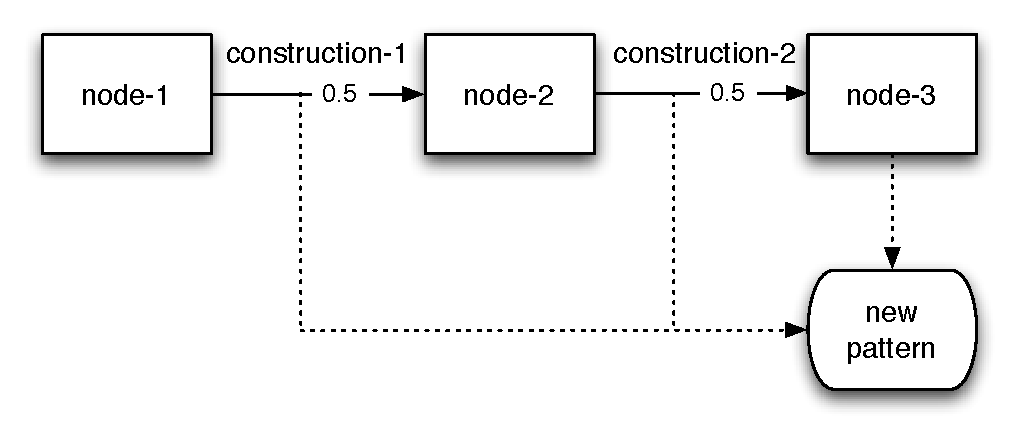
\includegraphics[width=0.8\textwidth]{Chapter4/figs/reaction1}}
  \caption[A reaction network\is{reaction network} as a source for pattern formation\is{formation}\is{pattern formation}]{An agent's reaction network\is{reaction network} is the source for pattern formation\is{pattern formation}. If the agents have to apply two constructions to license\is{license} an utterance (production) or a meaning (parsing), they will create a pattern based on the applied constructions. This pattern has the same functionality as the constructions but only requires one step.}
   \label{f:reaction1}
\end{figure}

Suppose that the agent is in production mode. In this case node-1 is the coupled feature structure\is{feature structure!coupled feature structure} which was license\is{license}d after unify\is{unify and merge}ing and merging the lexical entries for {\em jack, push} and {\em block}. Next, the speaker has to unify\is{unify and merge} and merge two constructions for marking the two participants of the push-event which license\is{license}s node-3. In a next step, which is not shown in the figure, the agent will unify\is{unify and merge} and merge the morphological rules. As indicated in the figure, this reaction network\is{reaction network} forms the basis for a new pattern (which will be construction-3). In principle this pattern should combine the entire reaction network\is{reaction network} including the lexical entries, but for convenience's sake the agents will only make a pattern which combines the functionality of constructions 1 and 2, as shown in Figure \ref{f:new-pattern}.
\begin{figure}[htb]
\centerline{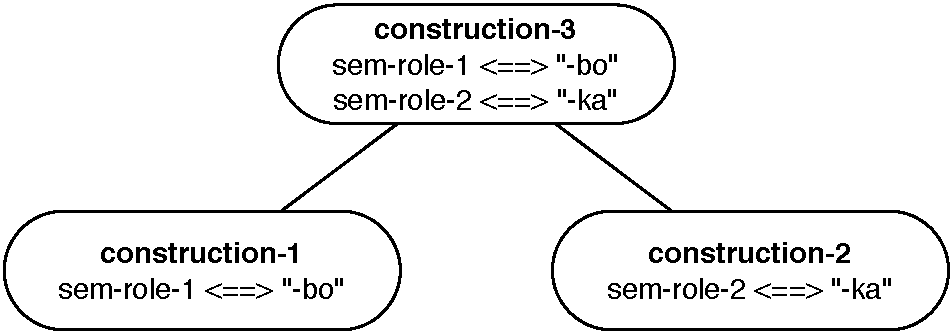
\includegraphics[width=0.8\textwidth]{Chapter4/figs/new-pattern}}
  \caption[A new pattern]{The two constructions that were used during processing are combined into a new construction. The agents keep a link between the new construction and the constructions that were used for creating it.}
   \label{f:new-pattern}
\end{figure}

The new construction is stored in the linguistic inventor\is{linguistic inventory}y with information about its origins: the agents keep a link between the new pattern and the constructions that were used for creating it. If the speaker has to produce the same meaning again, the new construction now forms an alternative path in the reaction network\is{reaction network}. The speaker will prefer this new path because it is faster in processing (one step can be skipped) and the links between the constructions can be used for giving priority to larger constructions if they unify\is{unify and merge} and merge. This new reaction network\is{reaction network} is illustrated in Figure \ref{f:reaction2}.
\begin{figure}[h]
\centerline{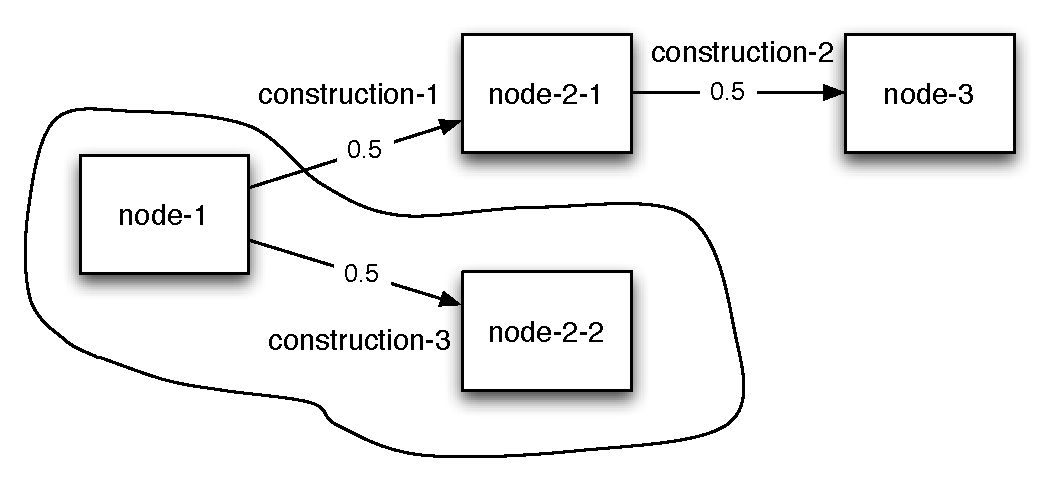
\includegraphics[width=0.8\textwidth]{Chapter4/figs/reaction2}}
  \caption[A reaction network\is{reaction network} with the new pattern]{The new construction now offers the agent an alternative path in the reaction network\is{reaction network}. Since the new pattern yields the same coupled feature structure\is{feature structure!coupled feature structure} as node-3 in only one step, it is faster and therefore preferred. The links between the three constructions are used to give larger patterns priority if they unify\is{unify and merge} and merge.}
   \label{f:reaction2}
\end{figure}

Apart from creating the new pattern, not much needs to be changed in the linguistic inventor\is{linguistic inventory}y apart from the fact that the agents have to link the new construction to the lexical entries that are compatible with it. The agents will not do this in one sweep but postpone this task until processing: lexical entries are only linked to the new construction instance by instance if this is required during a language game\is{language game}. The mechanism works entirely the same: the agent wants to unify\is{unify and merge} and merge two constructions and wants to optimize processing by creating a pattern. This time, however, no new pattern needs to be created because there is already one. The pattern thus exten\is{extension}ds its use to a new verb\is{verb} as well. The newly-made construction looks as follows:
\\
\\
{\footnotesize{\tt <Construction: construction-3
\\ ((?top-unit
\\ \hspace*{5mm} (sem-subunits (== ?unit-a ?unit-b ?unit-c)))
\\ \hspace*{2mm}(?unit-a
\\ \hspace*{5mm} (sem-frame (== (sem-role-1 ?unit-b ?obj-x)
\\ \hspace*{36mm}(sem-role-2 ?unit-c ?obj-y))))
\\ \hspace*{2mm}(?unit-b
\\ \hspace*{5mm} (referent ?obj-x))
\\ \hspace*{2mm}(?unit-c
\\ \hspace*{5mm} (referent ?obj-y))
\\ \hspace*{2mm}((J ?unit-b NIL)
\\ \hspace*{5mm} (sem-role sem-role-1))
\\ \hspace*{2mm}((J ?unit-c NIL)
\\ \hspace*{5mm} (sem-role sem-role-2)))
\\ <==>
\\ ((?top-unit
\\ \hspace*{5mm} (syn-subunits (== ?unit-a ?unit-b ?unit-c)))
\\ \hspace*{2mm}(?unit-a
\\ \hspace*{5mm} (syn-frame (== (syn-role-1 ?unit-b)
\\ \hspace*{36mm}(syn-role-2 ?unit-c))))
\\ \hspace*{2mm}(?unit-b
\\ \hspace*{5mm} (syn-role syn-role-1))
\\ \hspace*{2mm}(?unit-c
\\ \hspace*{5mm} (syn-role syn-role-2)))>}}
\\
\\
\noindent To summarize, the agents are equipped with the following diagnostic\is{learning strategies!diagnostics} and repair\is{learning strategies!repair strategies} strategy in all the experiments in this chapter:

\begin{enumerate}
\item {\bfseries Diagnostic:} If two constructions are used together for licensing a node in the network, report an opportunity for optimizing processing (both for production and parsing);
\item {\bfseries Repair strategy:} If there is a problem of processing effort: 
\begin{enumerate}
\item If a larger construction already exists for the same mapping, create a link between the lexical entry and the construction;
\item Else combine the two constructions into a new construction and keep a link between them.
\end{enumerate}
\end{enumerate}

During processing, the link between constructions is used for giving priority to larger constructions. They can also be used for consolidation\is{consolidation} as I will show in sections \ref{s:pattern-exp-2} and \ref{s:pattern-exp-3}. There are, however, no inheritance\is{inheritance} links: all relevant information is stored in the constructions themselves and no additional aspects are inherited from other constructions.

\section{Experiment 1: individual selection without analog\is{analogy}y}
\label{s:pattern-exp-1}

Before immediately picking up the experiments where the previous chapter left off, the influence of the diagnostic\is{learning strategies!diagnostics} and repair\is{learning strategies!repair strategies} strategy for pattern formation\is{formation}\is{pattern formation} is first tested for stage 2 in the development of case marker\is{case!case marking}s: the invention and adoption of specific marker\is{case!case marking}s.

\subsection{Experimental set-up}

The experimental set-up for experiment 1 is entirely the same as the one in baseline experiment 2c but this time the new diagnostic\is{learning strategies!diagnostics} and repair\is{learning strategies!repair strategies} strategy for pattern formation\is{formation}\is{pattern formation} are added to the agents. The set-up can be briefly summarized as follows:

\begin{itemize}
\item The population\is{speech population} consists of 10 agents that engage in description game\is{language game!description game}s;
\item The meaning space is the same one as detailed in Table \ref{t:events} and all event type\is{event type}s occur with the same frequency\is{frequency};
\item The agents have two diagnostic\is{learning strategies!diagnostics}s: detecting unexpressed variable equal\is{variable equality}ities and the new diagnostic\is{learning strategies!diagnostics} detecting whether two constructions were applied during processing;
\item The agents have two repair\is{learning strategies!repair strategies} strategies: one for inventing and learning verb\is{verb}-specific marker\is{case!case marking}s and one for combining them into a larger construction;
\item The agents use an alignment strateg\is{alignment strategy}y of direct competit\is{competition}ion which I will further call `individual selection'. This means that the hearer increases the confidence\is{confidence} scores of successfully applied constructions by 0.1 and decreases the scores of their direct competit\is{competition}ors by 0.1. The speaker does not perform score updating.
\end{itemize}

From the above follows that the agents will have to create and converge on one construction for each possible combination of meanings. There are thirty individual participant roles that need a single-participant construction, eighteen combinations of two participant roles and three combinations of three participant roles. Since the agents have no analog\is{analogy}y, the target number of constructions should be 51 (the sum of all these possibilities). All the combinations can be verified in the Appendix.

\subsection{Results and discussion}

\begin{figure}[tb]
\centerline{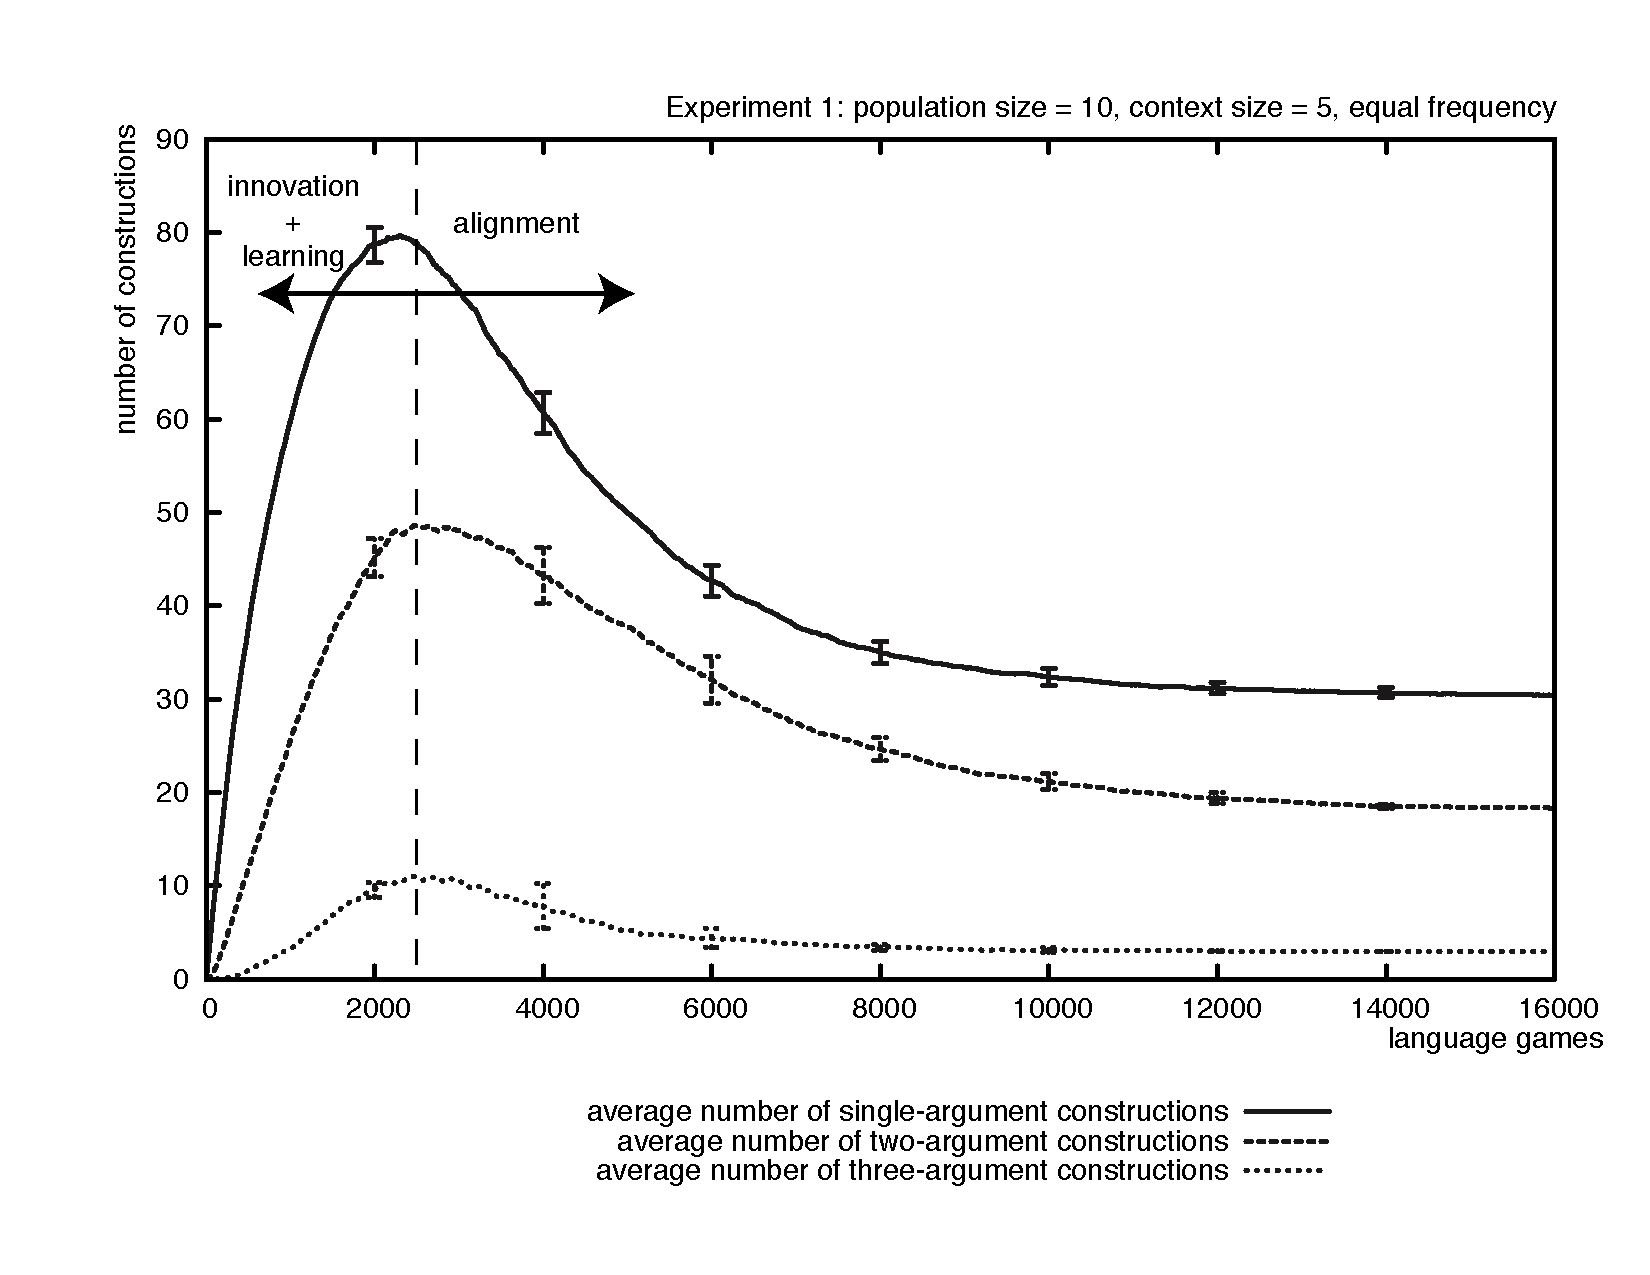
\includegraphics[width=0.85\textwidth]{Chapter4/figs/size2a}}
  \caption[Experiment 1: number of constructions with individual selection]{This graph shows the average number of constructions in a population\is{speech population} of ten agents in experiment 1. In this set-up the agents succeed in converging on an optimal inventory size -- given their cognitive abilities -- of 30 single-argument constructions, 18 two-argument constructions and 3 three-argument constructions. The graph here indicates that there is still an average of 19 two-argument constructions but this competit\is{competition}ion also gets resolved if more language game\is{language game}s are played.}
   \label{f:size1}
\end{figure}
\begin{figure}[htb]
\centerline{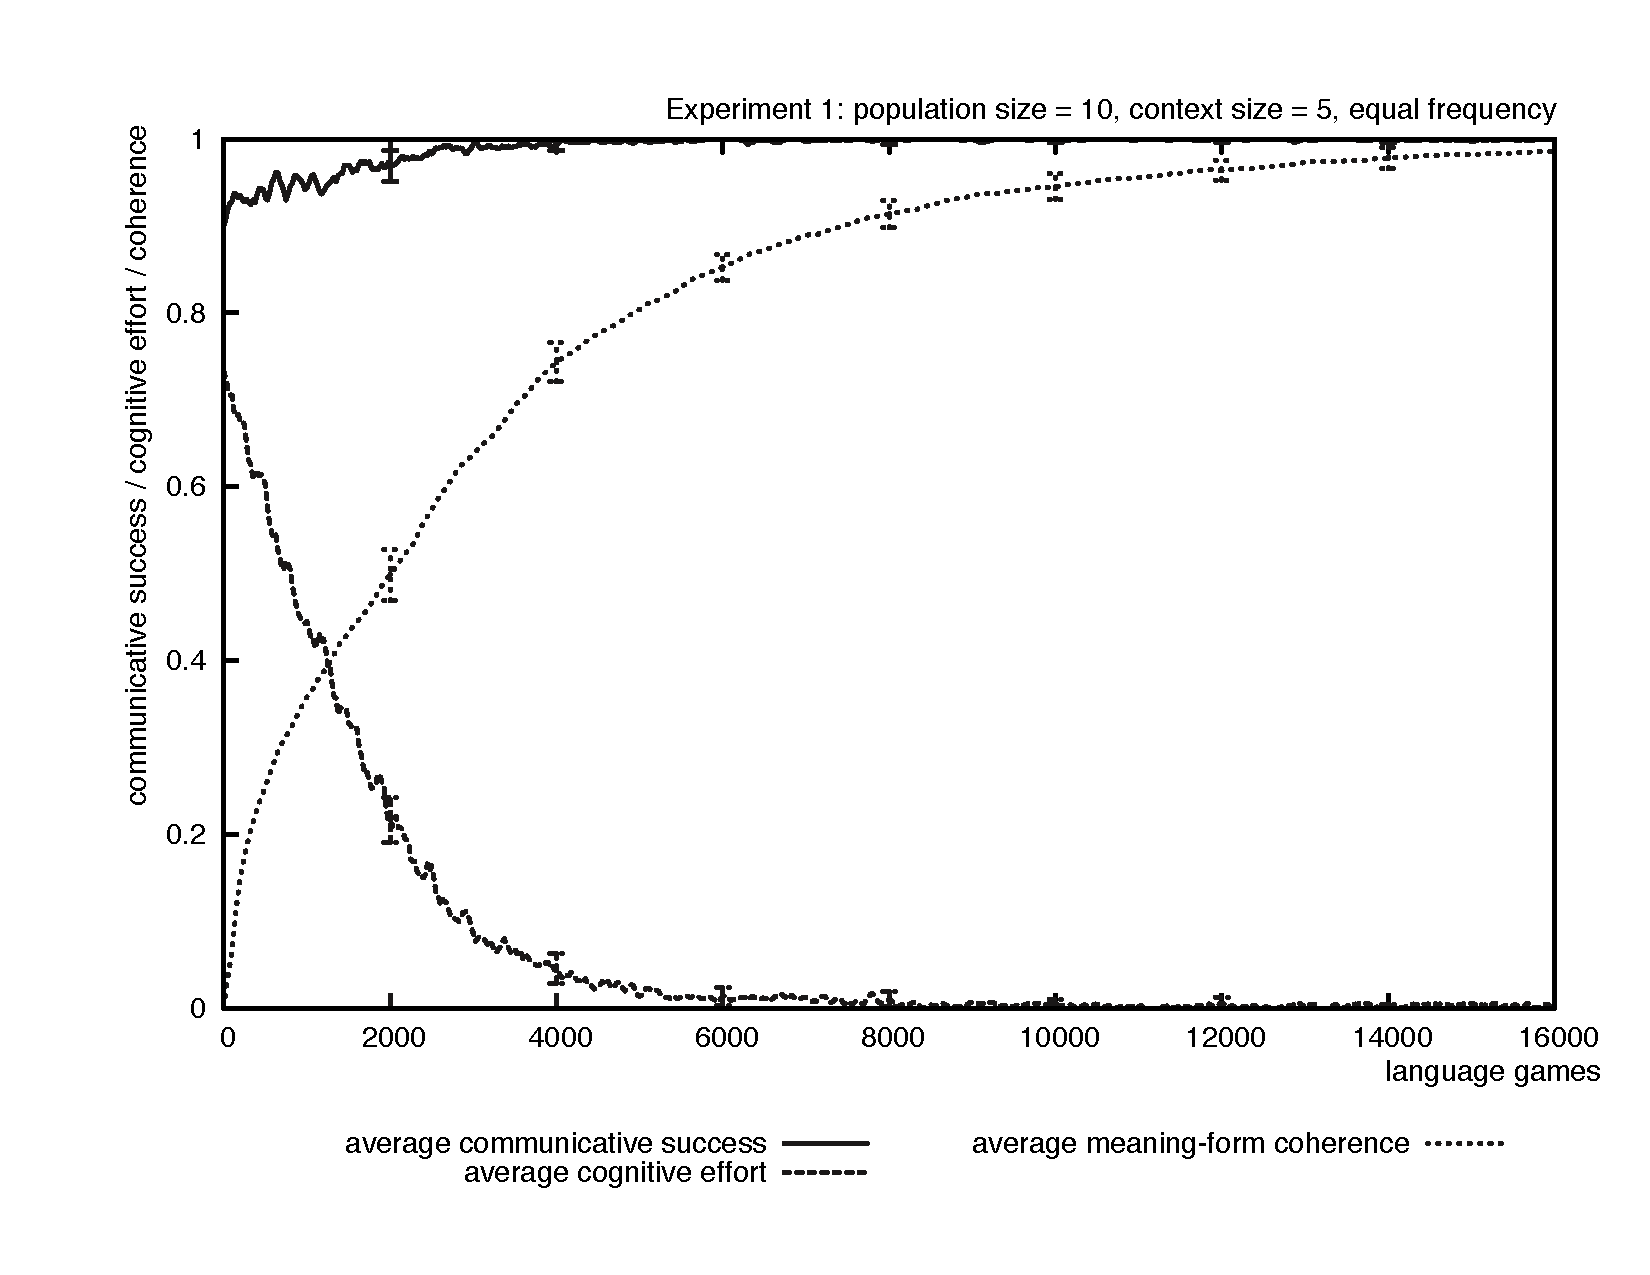
\includegraphics[width=0.85\textwidth]{Chapter4/figs/effort2a}}
  \caption[Experiment 1: success, effort and coherence]{This graph shows average communicative success\is{communicative success}, cognitive effort\is{cognitive effort} and meaning-form coherence in a population\is{speech population} of ten agents in experiment 1. The results show that the agents succeed in reaching 100\% communicative success\is{communicative success} and reducing the cognitive effort\is{cognitive effort} needed for communication. Meaning-form coherence reaches almost 100\% with only competit\is{competition}ion between one or two forms that is still undecided.}
   \label{f:effort1}
\end{figure}

\noindent{\bfseries Results.} The experimental set-up was tested in ten series of 16.000 language game\is{language game}s. By looking at the same measures as in the baseline experiments, the simulations seem to yield successful results at first sight. Figure \ref{f:size1} plots the average number of constructions in the population\is{speech population}. Here, the agents have almost reached the optimal state in terms of linguistic inventor\is{linguistic inventory}y. Only in the case of two-argument constructions there are additional language game\is{language game}s needed for deciding on the competit\is{competition}ion between one or two surviving constructions. Acquiring the constructions happens quite fast (in less than 3.000 games), but alignment takes much more time than was needed in the baseline experiments. This is due to the individual selection alignment strateg\is{alignment strategy}y: if a pattern was used, only competing patterns are punished through lateral inhibition\is{lateral inhibition}. The individual marker\is{case!case marking}s or rather the single-argument constructions they occur in are not considered during consolidation\is{consolidation}.
\begin{figure}[p]
\centerline{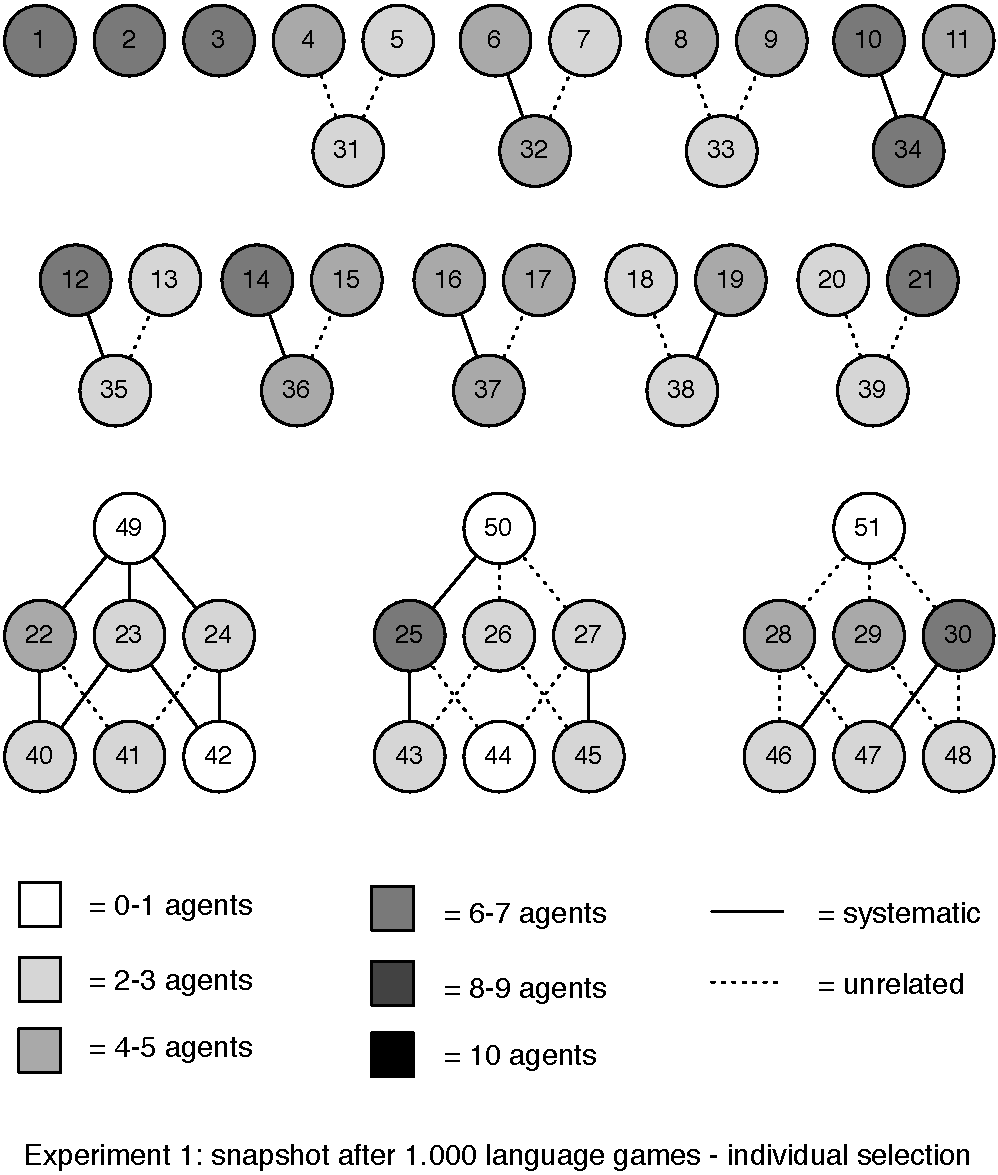
\includegraphics[width=0.7\textwidth]{Chapter4/figs/direct-coherence-no-analogy-1000}}
  \caption[Experiment 1: snapshot after 1.000 games]{This diagram gives a snapshot of the average coherence in a population\is{speech population} of 10 agents after 1.000 language game\is{language game}s using the direct selection alignment strateg\is{alignment strategy}y. Each circle stands for a particular meaning (see the Appendix), for example circles 4 and 5 stand for `appear-1' and `appear-2'. The lines between circles means that the meanings combine into compositional meanings, for example circle 31 means the combination `appear-1 appear-2'. The darker the circle is colour\is{colour}ed, the more agents prefer the same case marker\is{case!case marking}(s) for covering this meaning. A full line between circles means that both meanings are covered using the same marker\is{case!case marking}s (= systematic), a dotted line means that a different form is preferred for the same meaning (= unrelated). The diagram shows that for most meanings only half of the population\is{speech population} prefer the same form and that in many cases there is no systematic choice for a certain case marker\is{case!case marking}.}
   \label{f:1-coherence-1000}
\end{figure}

The long alignment period is also illustrated in Figure \ref{f:effort1}, which displays average communicative success\is{communicative success}, cognitive effort\is{cognitive effort} and meaning-form coherence. The fact that communicative success\is{communicative success} rapidly rises to 100\% within 4.000 language game\is{language game}s and that cognitive effort\is{cognitive effort} drops to zero between 6.000 and 8.000 language game\is{language game}s suggests that the agents have learned all the variation\is{variation}s floating around in their population\is{speech population}. However, meaning-form coherence takes much longer to rise to its maximum which is again due to the alignment strateg\is{alignment strategy}y. Coherence reaches almost 100\% after 16.000 games with only competit\is{competition}ion going on for one or two cases of two-argument constructions. This competit\is{competition}ion will in the end also be resolved after additional language game\is{language game}s.

The longer alignment period is however not the most fundamental problem with the artificial languages that are formed by the agents. A closer examination of them shows that all meaning-form mappings that they agree on are totally arbitrary. The problem is illustrated in Figures \ref{f:1-coherence-1000} and \ref{f:1-coherence-7000} which give a snapshot of convergence and coherence in one simulation after 1.000 and 7.000 language game\is{language game}s respectively. Each meaning or combination of meanings (see the Appendix) is represented as a circle. For example, the meaning `approach-1' is represented as circle 4 and meaning `approach-2' is represented as circle 5. Lines between circles indicate that the meaning of one circle is a combination of the meanings of the other circles. For example, circle 31 combines `approach-1' and `approach-2'. The colour\is{colour} of the circles represents the number of agents that prefer the most frequent form in the population\is{speech population} for that particular word. A white circle means that there is either no form yet for this meaning or that there is no form which is preferred by more than one agent. A black circle means that all ten agents prefer the same form for this meaning. If all the circles are black, the agents have reached 100\% convergence. If the lines between the circles are full lines, the same participant role is expressed by the same marker\is{case!case marking} across constructions. If however the line is dotted, there is a different form for the same meaning.

This can best be illustrated through an example. The circle for meaning 4 (approach-1) indicates that there are 4  or 5 agents in the population\is{speech population} which prefer the same form for marking this participant role at this stage of the simulation. For circles 5 (approach-2) and 31 (approach-1 approach-2), there are two or three agents that prefer the same form. The dotted lines between the circles, however, indicate that the most frequent pattern for circle 31 uses different marker\is{case!case marking}s than the single-argument constructions for circles 4 and 5:

\ea
\gll jack -lich approach\\
jack approach-1 approach\\
\glt `Jack approaches (someone)'.\\

\item
\gll jill -sut approach\\
jill approach-2 approach\\
\glt `(Someone) approaches Jill'.\\

\item
\gll jill -xa jack -zuih approach\\
jill approach-2 jack approach-1 approach\\
\glt `Jack approaches Jill'.\\
\z

\begin{figure}[p]
\centerline{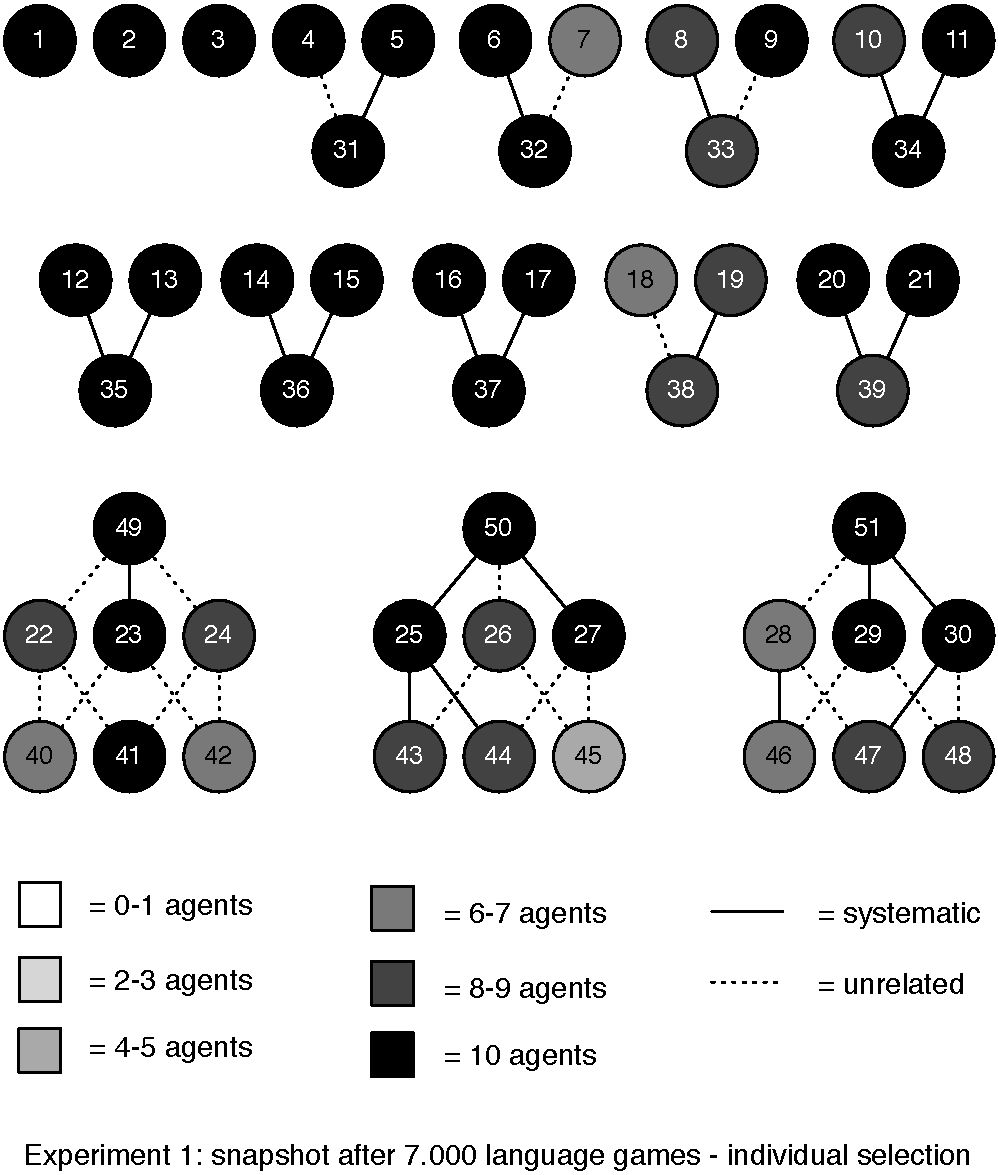
\includegraphics[width=0.7\textwidth]{Chapter4/figs/direct-coherence-no-analogy-7000}}
  \caption[Experiment 1: snapshot after 7.000 games]{This diagram gives a snapshot of the average coherence in a population\is{speech population} of 10 agents after 7.000 language game\is{language game}s using the direct selection alignment strateg\is{alignment strategy}y. The agents have reached convergence for most meanings by now, but these form-meaning mappings are not always systematically related to each other. For example, the meanings related to 49 were pretty consistent in their meaning-form mappings after 1.000 games, but have now become totally unrelated to each other: for each possible combination a new form is introduced to cover the same meaning. In all the cases where there is no systematicity\is{systematicity}, the convergence is not complete yet.}
   \label{f:1-coherence-7000}
\end{figure}

Figure \ref{f:1-coherence-7000} shows that after 7.000 language game\is{language game}s, the agents have almost converged on a form for every meaning, but the problem of systematicity\is{systematicity} remains: in half of the cases, a different case marker\is{case!case marking} is winning the competit\is{competition}ion on the level of single-argument constructions than the one(s) winning on the other levels. The figure also shows that in most of the cases where there is no systematic use of a form for the same meaning, convergence is also still not complete. This is in contrast to the meanings which (accidentally) arrived at the same form across constructions. Here we see mostly black circles meaning that all agents prefer the same convention\is{convention}.
\\
\\
\noindent{\bfseries Discussion.} The results clearly indicate that the agents are not capable of constructing a systematic language. The reason for this is that all constructions are basically treated as independent linguistic items. This means that once a larger pattern is created, it starts living its own life without influencing or being influenced by the constructions that were used to create it. This results in some case marker\is{case!case marking}s losing the competit\is{competition}ion for marking a certain participant role on the level of single-argument constructions but still becoming the most successful one as part of a larger pattern. In all the simulations, this happened in 40 to 60\% of the cases (see Figure \ref{f:systematicity2}).

The fact that in more than half of the cases the same marker\is{case!case marking} wins the competit\is{competition}ion on all levels is due to the small meaning space of the experiment and the fact that patterns are always created by combining the most successful constructions at a given point in the simulation. In fact, the agents can continue to create new patterns for a certain combination of participant roles even if they already know other patterns for it. For example, it may happen that on a lower level the average confidence\is{confidence} scores of a new combination becomes more successful than the confidence\is{confidence} score of the patterns. In this case the agents will still innovat\is{innovation}e which gives a slight advantage to those patterns that are in line with the most successful constructions of a lower level. As the results show, however, this is not enough.

Since natural languages are also not fully regular, it is important to see whether the lack of systematicity\is{systematicity} in the experiments is relevant for the many exceptions and sub-regularities found in natural languages. The answer is no: for most if not all irregular forms and sub-regularities in natural language, either a systematic origin can be found through diachron\is{diachronic}ic changes or through external pressures such as language contact\is{language contact}. For example, the -ed-participle in English\is{English} did not manage to exten\is{extension}d its use to all past tense\is{tense}s as can be observed in irregular verb\is{verb}s such as {\em to sing} and {\em to give}. These strong verb\is{verb}s are however remnants of completely regular classes of verb\is{verb}s in Proto-Indo-European that were able to survive thanks to their high token frequency\is{token frequency}\is{frequency}. Despite all sociological factors, historical incidents, language contact\is{language contact}, and other kinds of exceptions, natural languages succeed remarkably well in developing systematicity\is{systematicity} spanning over many constructions, as for example word order in English\is{English}. Given the abstraction\is{abstraction}s and scaffold\is{scaffold}s of the present experiments, the agents should thus be capable of developing a fully systematic language without any problems.

This leaves us the question of how systematicity\is{systematicity} can be achieved. As said before, all systematic form-meaning mappings have been formed by accident due to the small world and the nature of the innovat\is{innovation}ion mechanism. For true systematicity\is{systematicity}, however, the agents need to be able to recognize relations between constructions rather than treating them as a list of independent units. This would mean that if a particular construction is successful, its systematically related constructions should also (perhaps indirectly) benefit from its success. In section \ref{s:pattern-exp-2} I will introduce a biologically inspired mechanism that can be exploited to achieve this effect: multi-level selection\is{multi-level selection}.

\subsection{The problem of systematicity\is{systematicity} in other work}
\label{s:problem-systematicity}

As to my knowledge, the problem of systematicity\is{systematicity} has never been reported before in the field of the origins\is{origins} and evolution\is{evolution!cultural evolution} of language. This does not mean, however, that the problem never existed. In this section, I will give a brief overview of some prior work in the field in which the problem was either overlooked or in which it could not occur due to experimental assumption\is{assumption}s.
\\
\\
\noindent{\bfseries Exemplar-based\is{exemplar-based models} simulations.} One computational simulation which is closely related to the work in this book is presented by \citet{batali02negotiation}. Batali investigates how a multi-agent population\is{speech population} can form a recursi\is{recursion}ve communication system by using exemplars stored in memory. This work can be categorized as a `problem-solving\is{problem-solving} model' because these exemplars have to be agreed upon in locally situated interactions. Each exemplar has a confidence\is{confidence} score which is increased and decreased according to similar lateral inhibition\is{lateral inhibition} dynamics as in the simulations of the previous section. The type of learner is thus the same one as the agents in this book: they build their language instance by instance in a bottom-up and redundant fashion. Batali's agents only keep exemplars and all generalization in the model is captured by directly manipulating these exemplars during processing. Figure \ref{f:batali} gives an example of an exemplar composed of two smaller ones \citep[exemplar 5.1.2.a]{batali02negotiation}.
\begin{figure}[h]
\centerline{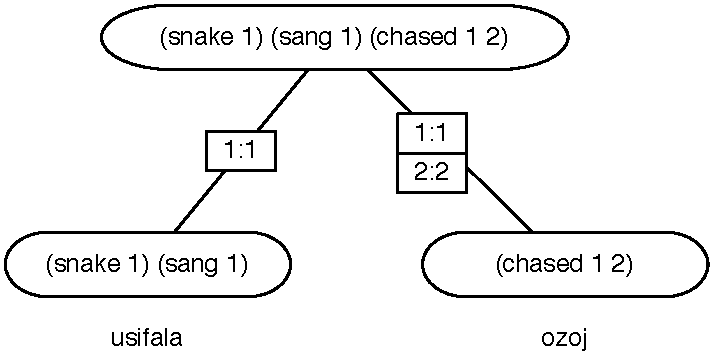
\includegraphics[width=0.75\textwidth]{Chapter4/figs/batali}}
  \caption[An exemplar \citep{batali02negotiation}]{A complex exemplar from \citet{batali02negotiation}. The exemplar features a compositional meaning with `argument maps' to the smaller exemplars that take care of variable equal\is{variable equality}ities in the meaning.}
   \label{f:batali}
\end{figure}

Batali does not use event-specific variables as I do in this book but assumes a simple three-way contrast between arguments 1, 2 and 3. For example the meaning ((snake 1) (sang 1)) translates to something like `the snake sang', whereas ((snake 1) (sang 2)) would mean something like `there was a snake and something sang.' Event structure\is{event structure} is stored immediately in the exemplar but can be overridden by argument maps between complex exemplars and their subcomponents. For example, the argument map `1:2' translates a meaning like (rat 1) to (rat 2). These argument maps are also stored as part of the complex exemplar. Apart from these argument maps between complex exemplars and their components, all exemplars are unrelated and listed in the memory.

The agents then engage in a series of description game\is{language game!description game}s. They are able to invent new words for new meanings and they are capable of combining existing words into larger patterns or breaking up a pattern again into smaller parts. The ultimate goal of the agents is two-fold: (a) agree on a shared lexicon\is{lexicon} for all the single meanings (e.g. cat, fox, chase, etc.) and (b) agree on a way to mark event structure\is{event structure} through the argument maps (i.e. marking the difference between arguments 1, 2 and 3). The simulations make use of a single generation of agents.

The results indicate that the agents gradually reach communicative success\is{communicative success} and that they agree on the same exemplars. Goal (a) is therefore definitely reached. However, the results show that event structure\is{event structure} is not always marked in the same way: all the simulations end up using specific ordering for each exemplar (even though they may involve the same meanings) and using `empty' words that accidentally evolved into marker\is{case!case marking}s for argument mappings. The agents thus do not succeed in agreeing on a systematic way of distinguishing participant `1' from participants `2' and `3'. The agents thus cannot generaliz\is{generalization}e argument mapping to new predicates such as (give 1 2 3) and have to negotiat\is{negotiation}e event structure\is{event structure} for each word separately. This lack of systematicity\is{systematicity} is not noted by Batali as a problem and the use of the empty words is wrongly interpreted as corresponding to argument marker\is{case!case marking}s in natural languages.
\\
\\
\noindent{\bfseries Probabilistic grammars.} Another experiment in which the systematicity\is{systematicity} problem is overlooked is reported by \citet[chapter 10]{depauw02grael}. De Pauw investigates how rudimentary principles of syntax can emerge from distributional aspects of communication rather than from the interface\is{syntax-semantics interface} between syntax and semantics. This exclusive focus on syntax is different from the work in this book (even though some semantics is smuggled into De Pauw's simulations in the disctinction between animate\is{animacy} and non-animate\is{animacy} objects which results in different distributional patterns). Similar assumption\is{assumption}s to this book are the heavy use of memory (even more so by De Pauw), a bottom-up and redundant formation\is{formation} of the language and a predefined lexicon\is{lexicon} in order to focus exclusively on the topic of interest. The population\is{speech population} in De Pauw's simulations is dynamic in the sense that there is a generational turn-over, but no linguistic information is transmitted genetically from one generation to the next.

The agents engage in a series of language game\is{language game}s in which they communicate about objects or events. If there are several objects, the agents can choose between six word orders: SVO, SOV, VSO, VOS, OSV or OVS. De Pauw therefore does not distinguish between verb\is{verb}-specific participant roles, but only assumes a two-way contrast between the subject\is{syntactic role!subject} (S) and the object\is{syntactic role!object} (O). The agents start without any preference for a particular word order so variation\is{variation} naturally occurs in the population\is{speech population}. The alignment strateg\is{alignment strategy}y of the agents is simply storing bigrams or frequencies of co-occur\is{co-occurrence}rences and performing statistical inducti\is{induction}on on top of those bigrams \citep[362]{depauw02grael}:
\begin{figure}[h]
\centerline{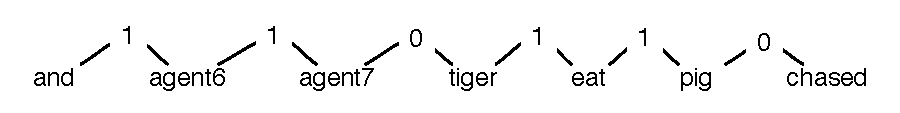
\includegraphics[width=\textwidth]{Chapter4/figs/depauw}}
  \caption[Bigram probabilities \citep{depauw02grael}]{The agents in \citet{depauw02grael} store co-occur\is{co-occurrence}rence frequencies and use these bigram-probabilities to decide on a preferred ordering.}
   \label{f:depauw}
\end{figure}

During the simulations, the agents rapidly converge on fixed word order on simple relations. However, as De Pauw notes, there are no general tendencies in terms of a general word order. Each `verb' rather has its own preferred ordering. For more complex relations, the agents do not always reach coherence. De Pauw concludes that the agents therefore reside in a local maximum and that they evolve from one local maximum of convergence to the next. De Pauw argues that this is not a shortcoming of the model but rather its greatest asset: whereas other models in the field are looking for the state of convergence, {\em ``language itself never converges and constantly adapts to a changing environment and seems to be driven by chaotic elements, introducing a large degree of randomness in language both from a synchron\is{synchronic}ic, as well as a diachron\is{diachronic}ic point of view''} (p. 378).

There are however no such chaotic elements present in De Pauw's model which should prevent the agents from reaching complete coherence. The degree of randomness in his simulations seems to stem from the systematicity\is{systematicity} problem: by only looking at bigram probabilities, it is to be expected that there is an arbitrary word order which is verb\is{verb}-specific. In the case of more complex predicates, the preferred order depends on a combination of various bigrams which increases the randomness because the probabilities of these bigrams are constantly changing so it becomes much harder to agree on a fixed order for these complex meanings. De Pauw dismisses the possibility that the degree of convergence is the maximum that can be expected from the population\is{speech population}, but this is in fact the only correct conclusion. Given the cognitive capabilities of the agents, convergence could only increase if the input would be more structured. In certain machine learning\is{machine learning} tasks, there is already a lot of structure present in the learning data so bigrams can be successfully used for making some predictions. In the case of language formation\is{formation}, however, agents have to start from scratch so there is no structure spanning multiple levels yet that can be induced.

De Pauw's concluding remark is that it is empirically impossible to know whether the agents succeed in {\em ``expressing the proper (agent, patient) relationship, or if it is just a side-effect of beneficial bigram probability distributions''} (p. 376). I would argue, however, that since the agents are not endowed with the capacity of relating bigrams to each other but solely rely on these probabilities, all tendencies in word order are in fact a side-effect of the bigrams. The conclusion is that \citet{depauw02grael}, just like \citet{batali02negotiation}, misinterpreted experimental results because the problem of systematicity\is{systematicity} was not noticed.
\\
\\
\noindent{\bfseries Iterated Learning Model\is{Iterated Learning Model (ILM)}s.} So far I only discussed models that featured lazy learner\is{lazy learner}s: agents which postpone generalization until processing time and which shape their language in a step-by-step fashion. As opposed to lazy learner\is{lazy learner}s there are `eager learner\is{eager learner}s'. Eager learner\is{eager learner}s try to look for generalizations (and abstraction\is{abstraction}s) before it is actually needed in processing and work on the complete inventory. Eager learner\is{eager learner}s typically discard the examples that can be deriv\is{derivation}ed from a rule and thus try to optimize the inventory size. If the problem of systematicity\is{systematicity} also occurs with eager learner\is{eager learner}s, then we know that the problem is not exclusive to the usage-based approach\is{usage-based model} proposed in this book. 

In the field of artificial language evolution\is{artificial language evolution}, especially Iterated Learning Model\is{Iterated Learning Model (ILM)}s feature agents that loop through their inventory after each interaction in order to make abstraction\is{abstraction}s. In section \ref{s:impact} I will draw a thorough comparison between my experimental results and those of \citet{moy06case}, who investigated the same topic using the Iterated Learning Model\is{Iterated Learning Model (ILM)} so I will not go into details here. As a quick preview, I can already give away one of the conclusions which is that the problem of systematicity\is{systematicity} also occurs in Iterated Learning Model\is{Iterated Learning Model (ILM)}s. This does not only happen in Moy's experiments, but also in the simulations reported by \citet{kirby00syntax} and \citet{smith03iterated} even though these models feature complete meaning transfer and a population\is{speech population} of only two agents.

The conclusion is the same as for the other simulations reported in this section: the problem of systematicity\is{systematicity} goes by unnoticed in most Iterated Learning Model\is{Iterated Learning Model (ILM)}s, but becomes very apparent in \citet{moy06case}. The problem occurs for the same reasons as in all the other experiments: the agents only behave `systematic' during innovat\is{innovation}ion and learning, but then treat all linguistic items as an unstructured list of unrelated elements. So either there is no adequate model yet that avoids the problem of systematicity\is{systematicity} or the problem is {\bfseries not restricted to the type of learner}. In the latter case, the problem seems to be caused by the fact that the linguistic inventor\is{linguistic inventory}y is unstructured.
\\
\\
\noindent{\bfseries Other models.} Finally, there are many models that investigate certain aspects of grammar in which the problem of systematicity\is{systematicity} does not occur such as \citet{debeule07compositionality, debeule06emergence, nowak99evolution, steels06how-grammar}; etc. I will take the simulations by \citet{debeule06emergence} as an example of why these models don't have the problem. The conclusions of this brief discussion extend to all the other models on grammar as well.

De Beule \& Bergen investigate the competit\is{competition}ion between holistic and compositional utterances. In case of compositional utterances, one could expect the problem of systematicity\is{systematicity} to pop up, but it doesn't. The reason is that De Beule \& Bergen designed their experiment in such a way that the agents had prior knowledge about what kind of categories and constructions to expect: individual words are immediately tagged with a certain syntactic category and grammatical constructions are fully schematic from the start. One construction can hence be used for all possible combinations of competing individual words that are tagged with the same category and remains agnostic as to which words should win the competit\is{competition}ion. The experiment thus made a clear separation between the lexicon\is{lexicon} on the one hand and grammatical constructions on the other; and it did not offer the agents the possibility of in-between patterns or idiom\is{idiom}s.

This is not a criticism of the model per se: given the fact that De Beule \& Bergen only intended to focus on competit\is{competition}ion between holistic and compositional utterances, the design choice is justified in which the competit\is{competition}ion dynamics can be clearly investigated on each level. As such the experiment can be interpreted as investigating a prerequisite of grammar rather than the emergence\is{formation} of {\em actual} grammar. For the scope of this book, this experimental design is thus not warranted: the barrier between fully idiom\is{idiom}atic items and fully schematic items needs to be broken down.

\section{Experiment 2: multi-level selection\is{multi-level selection} without analog\is{analogy}y}
\label{s:pattern-exp-2}

In the previous section I demonstrated the problem of systematicity\is{systematicity} that occurs during the emergence\is{formation} of a language if the agents treat all entries in their linguistic inventor\is{linguistic inventory}y as unrelated individuals and if their language comprises multiple layers of organization. An alignment strateg\is{alignment strategy}y involving the individual selection of constructions leads to completely arbitrary form-meaning pairs whereas natural languages show greater cohesion and a higher degree of systematically related constructions. Even in idiom\is{idiom}s such as {\em he kicked the bucket}, some degree of schematicity is present such as the conjugation of the verb\is{verb}. The agents therefore need a new alignment strateg\is{alignment strategy}y in which the success of one construction may have an impact on the success of other related constructions.

In this section I will present an experiment which features new alignment strateg\is{alignment strategy}ies that are inspired by the notion of `multi-level selection\is{multi-level selection}' in evolutionary biology \citep{wilson94group}. Multi-level selection\is{multi-level selection} (formerly known as `group selection') acknowledges the fact that groups or other higher-level entities can act as `vehicles' for selection. In this view, not all aspects of groups are reduced to by-products of individual (and usually selfish) interactions. In other words, being part of a group can increase the selectionist advantage of individuals.% One example from biology concerns the origins of chromosomes. Individual genes started to be combined into larger units (chromosomes). The genes are on the one hand replicators in their own right, undergoing competit\is{competition}ion, but they are also part of the larger replicating unit of chromosomes \citep{maynard-smith93origin}.

Natural languages are clear instances of organisms with a hierarchical functional organization which can be conceived as `groups within groups'. Competition is going on at multiple levels of this organization: between synonyms for becoming dominant in expressing a particular meaning, between idiom\is{idiom}atic patterns that group a number of words, between different syntactic and semantic categories competing for a role in the grammar, between ways in which a syntactic category is marked, etc. Multi-level selection\is{multi-level selection}s therefore seems to be readily applicable to language as well.

\subsection{Experimental set-up}

The most important requirement for implementing multi-level selection\is{multi-level selection} is that the agents have to be capable themselves of recognizing relations between linguistic items. This is in fact not so difficult to achieve: in section \ref{s:operationalizing-patterns} I explained that the agents keep a link between larger constructions and the constructions that were used for creating them. These links can now be used for implementing multi-level selection\is{multi-level selection}. Three different alignment strateg\is{alignment strategy}ies have been implemented for comparison:

\begin{itemize}
\item {\bfseries Top-down selection}: if the game was a success, the hearer will not only reward the constructions that were applied during processing, but also all the related constructions on a lower level. The confidence\is{confidence} scores of all the competit\is{competition}ors of these constructions are decreased through lateral inhibition\is{lateral inhibition}.
\item {\bfseries Bottom-up selection}: If the game was a success, the hearer will not only increase the score of the applied constructions, but also the scores of all the related constructions on a higher level. All the competing constructions are punished.
\item {\bfseries Multi-level selection\is{multi-level selection}}: If the game was a success, the hearer will not only increase the score of the applied constructions, but also the scores of all related constructions. All the competing constructions are punished through lateral inhibition\is{lateral inhibition}.
\end{itemize}

Retrieving related constructions is performed recursi\is{recursion}vely. For example, if a three-argument construction was applied using the top-down selection alignment strateg\is{alignment strategy}y, its two sub-components are retrieved (a two-argument and a single-argument construction) as well as the two sub-components of the two-argument construction. The hearer thus increases the scores of five constructions. The competit\is{competition}ors are all the direct competit\is{competition}ors of these five constructions.
\begin{figure}[p]
\centerline{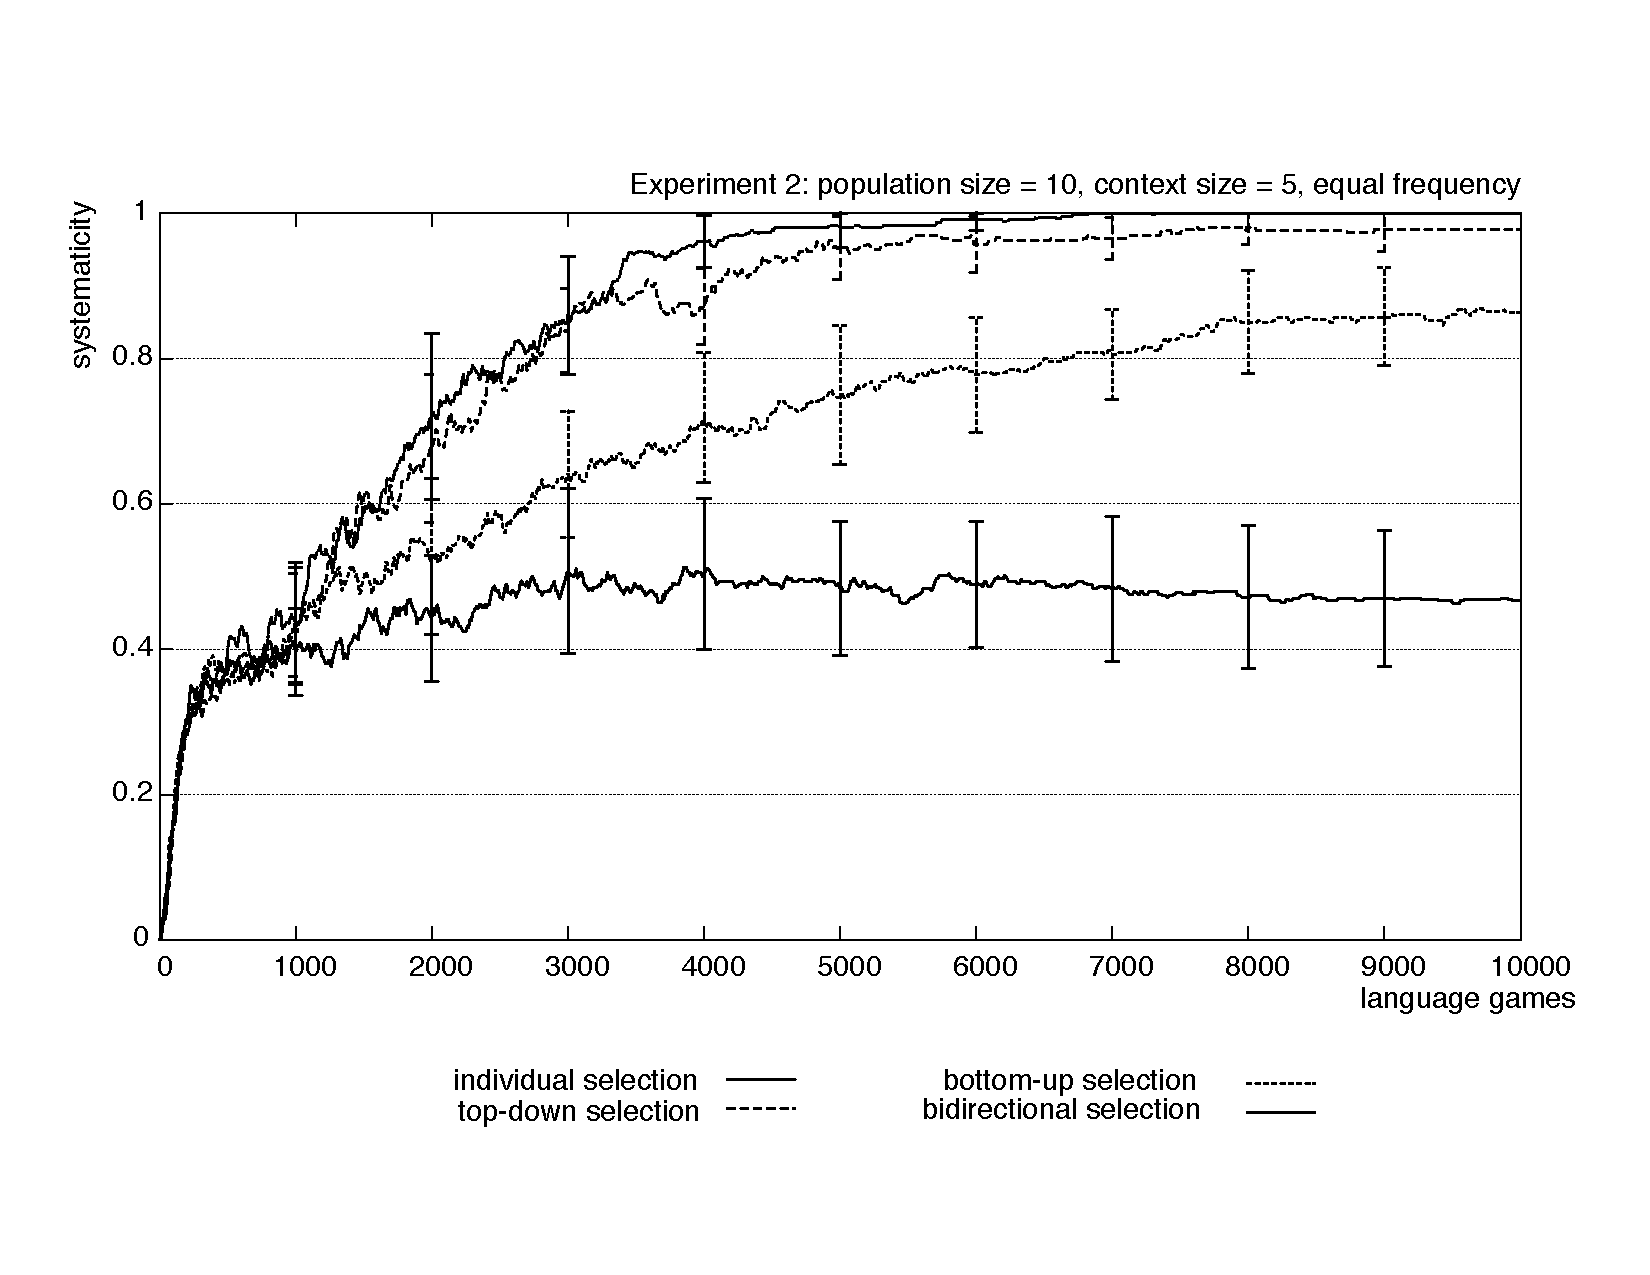
\includegraphics[width=\textwidth]{Chapter4/figs/systematicity-vs-2}}
  \caption[Experiment 2: systematicity]{This graph compares the performance\is{performance} in terms of systematicity\is{systematicity} of four experimental set-ups. systematicity\is{systematicity} fluctuates around 50\% in the baseline case where there is only individual selection (experiment 1). With the bottom-up selection strategy the agents improve the systematicity\is{systematicity} rate to 80\% but then get stuck. Top-down selection leads to full systematicity\is{systematicity} in some of the runs, but most of the simulations feature some `frozen accidents' as well. Only the multi-level selection\is{multi-level selection} strategy leads to full systematicity\is{systematicity} in all the series after about 7.000 language game\is{language game}s.}
   \label{f:systematicity2}
\end{figure}

During processing, only the scores of the applied constructions are taken into account and not of the whole group of related constructions. The group selection dynamics therefore only matter during consolidation\is{consolidation}. The rest of the set-up is the same as for experiment 1.

\subsection{Results and discussion}

\begin{figure}[p]
\centerline{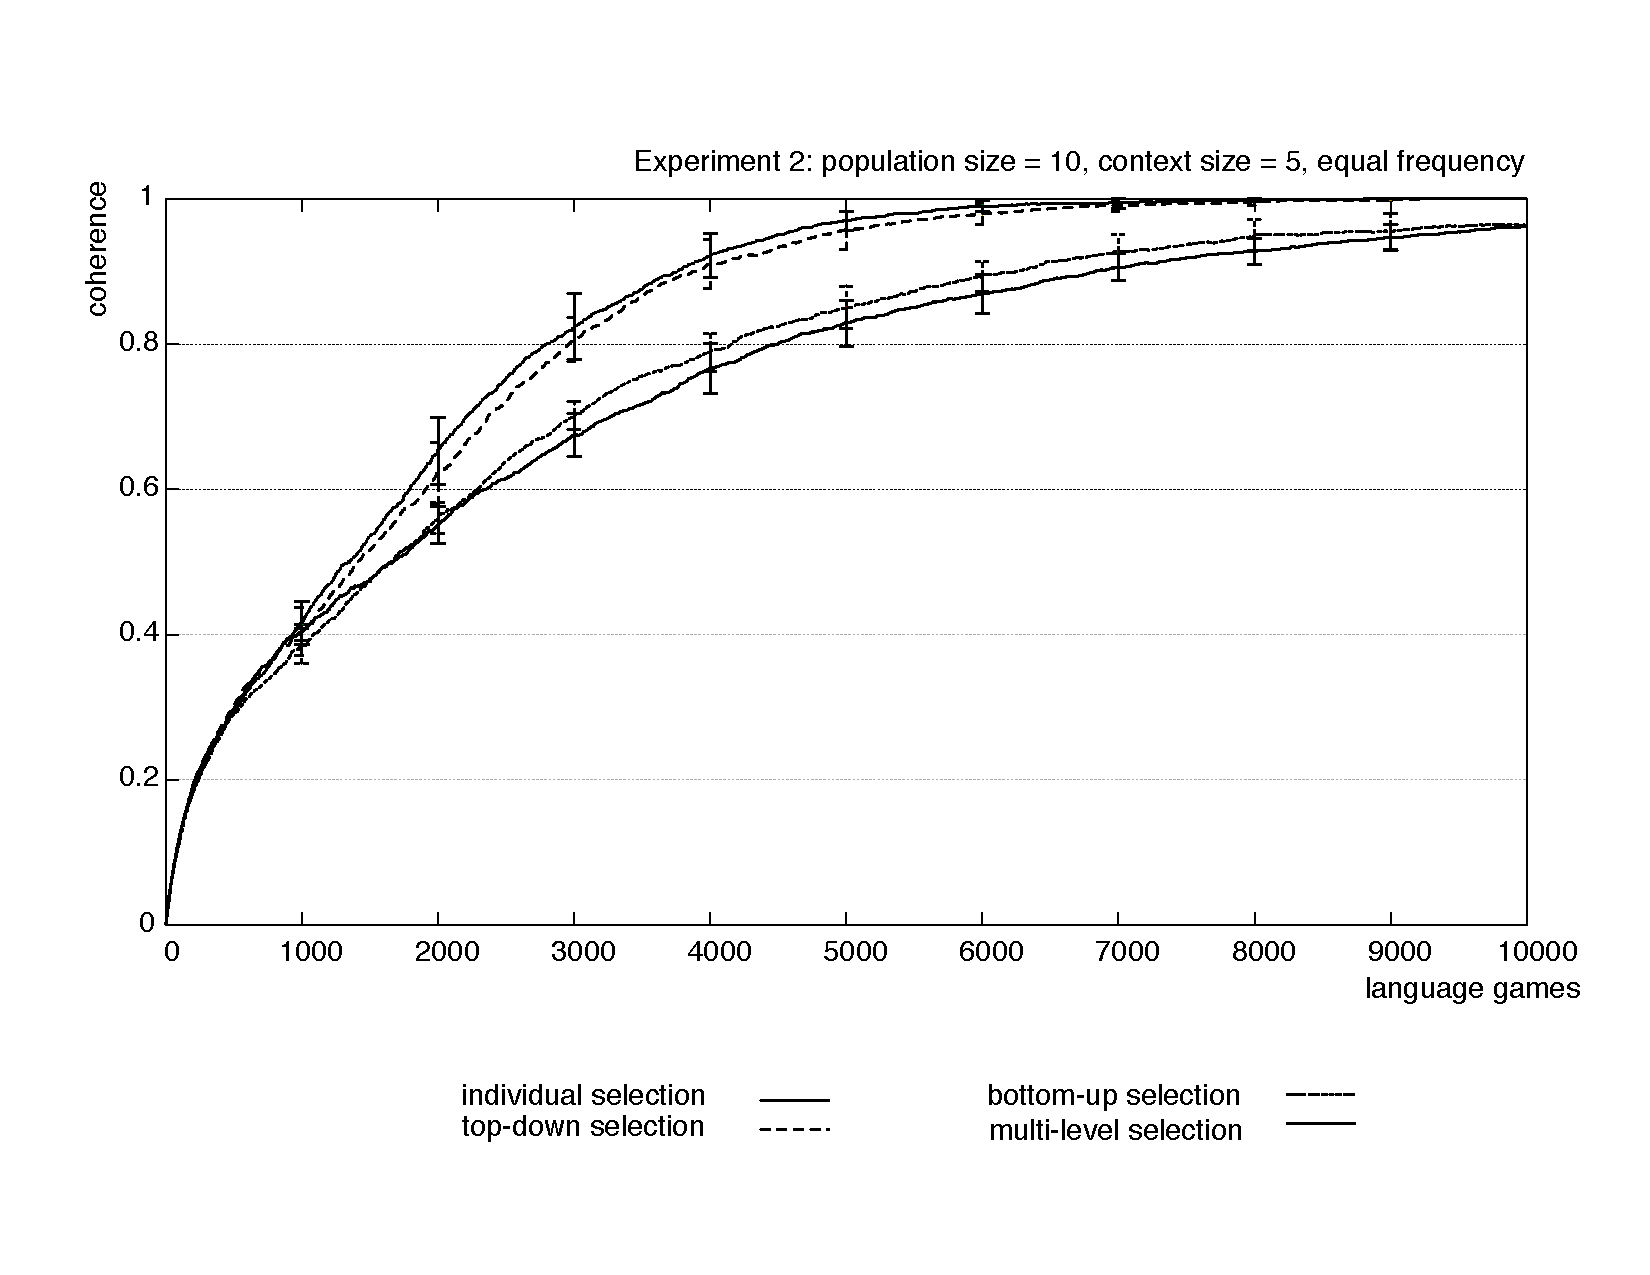
\includegraphics[width=\textwidth]{Chapter4/figs/coherence-vs-2}}
  \caption[Experiment 2: meaning-form coherence]{Since the systematicity\is{systematicity} graph only takes the most frequent forms into account, meaning-form coherence has to be checked in order to verify whether all the agents have converged on the same form-meaning pairs. We see that after 10.000 language game\is{language game}s, only the top-down and the multi-level selection\is{multi-level selection} alignment strateg\is{alignment strategy}ies have already reached complete coherence. Multi-level selection\is{multi-level selection} slightly outperforms top-down selection but not significantly so. In the case of bottom-up and individual selection, the agents need additional language game\is{language game}s for reaching coherence.}
   \label{f:coherence2}
\end{figure}

The three alignment strateg\is{alignment strategy}ies were compared to each other and to experiment 1 in ten series of 10.000 language game\is{language game}s.
\\
\\
\noindent{\bfseries Results.} Figure \ref{f:systematicity2} illustrates the amount of systematicity\is{systematicity} in all four alignment strateg\is{alignment strategy}ies. The graph shows that the three alignment strateg\is{alignment strategy}ies involving multiple levels all improve on the baseline of individual selection of experiment 1. With the alignment strateg\is{alignment strategy}y of individual selection, systematicity\is{systematicity} fluctuates between 40 and 60\% depending on how `lucky' the agents were. The behaviour of the other three strategies is much more consistent over the ten series. The graph shows that bottom-up selection allows the agents to improve systematicity\is{systematicity} to 80\% but there they are faced with `frozen accidents' as well. The top-down selection improves systematicity\is{systematicity} even further and allows the agents to reach full systematicity\is{systematicity} in some of the runs. However, in most cases, there were still two or three unsystematic patterns left. Only the multi-level selection\is{multi-level selection} strategy led to full systematicity\is{systematicity} in all the simulations.

Since the measure of systematicity\is{systematicity} only looks at the most frequent forms floating in a population\is{speech population}, it needs to be complemented with meaning-form coherence to verify whether {\em all} the agents converge on the same preferences. Figure \ref{f:coherence2} therefore compares the performance\is{performance} of the four alignment strateg\is{alignment strategy}ies in terms of coherence. From the results of experiment 1 we already knew that in the case of individual selection, alignment takes longer than 10.000 language game\is{language game}s. The coherence line for bottom-up selection runs almost parallel with it and does not improve on it in terms of convergence speed. The only two strategies that reach convergence within 10.000 games are top-down and multi-level selection\is{multi-level selection}. Full coherence in the case of top-down selection however does not mean full systematicity\is{systematicity}, as was shown in Figure \ref{f:systematicity2}.
\begin{figure}[t]
\centerline{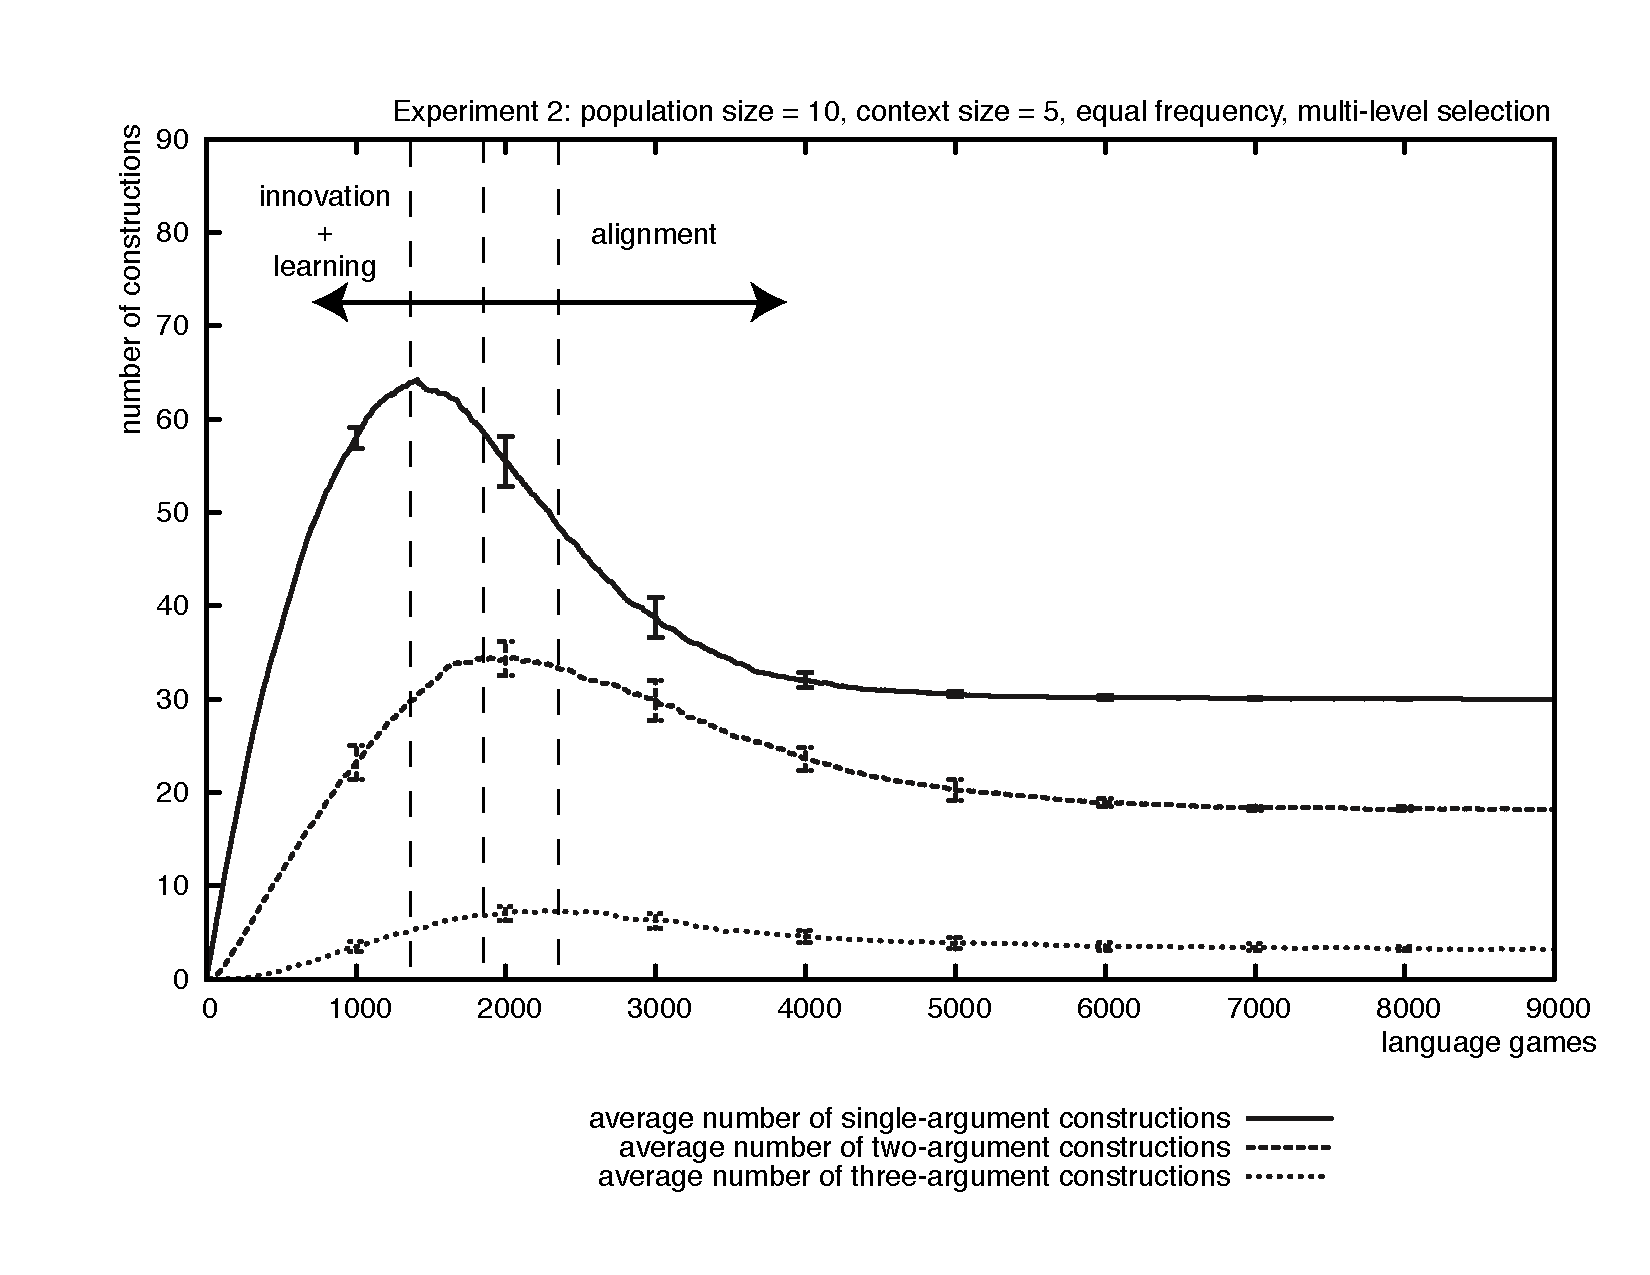
\includegraphics[width=0.87\textwidth]{Chapter4/figs/size2d}}
  \caption[Experiment 2: number of constructions with multi-level selection\is{multi-level selection}]{This graph shows the average number of constructions known by an agent using the multi-level selection\is{multi-level selection} alignment strateg\is{alignment strategy}y. Compared to individual selection, multi-level selection\is{multi-level selection} allows the agents to discard competit\is{competition}ors much more rapidly: there are significantly less variation\is{variation}s floating around in the population\is{speech population}. For example, the peak of single-argument constructions is about 60 instead of 80 in experiment 1. Also the alignment phase happens much faster.}
   \label{f:size2d}
\end{figure}

Figure \ref{f:size2d} shows the average number of constructions in the ten series involving the alignment strateg\is{alignment strategy}y of multi-level selection\is{multi-level selection}. The graph confirms the fact that the agents converge significantly faster on an optimal number of constructions than in experiment 1. At the peak of competing constructions, there are about 60 single-argument constructions, 30 two-argument constructions and 6 three-argument constructions or an average of two competing constructions for each possible meaning. This is much less than in experiment 1 (see Figure \ref{f:size1}) which featured peaks of 80 single-argument, 50 two-argument and 10 three-argument constructions. Also alignment happens much faster: with multi-level selection\is{multi-level selection}, the agents align after 6.000 games as opposed to 14.000 language game\is{language game}s or more if the agents use individual selection.

Figures \ref{f:2d-coherence-1000} and \ref{f:2d-coherence-7000} offer a snapshot of the most frequent forms in a population\is{speech population} using the multi-level selection\is{multi-level selection} alignment strateg\is{alignment strategy}y. Both snapshots confirm the results indicated by the coherence and systematicity\is{systematicity} graphs. Figure \ref{f:2d-coherence-1000} shows already much more dark grey circles than Figure \ref{f:1-coherence-1000} featuring individual selection, indicating that for most meanings there is already a majority of agents preferring the same form. The preferred forms are also to a higher degree systematically related to each other than in experiment 1, even for the more complex patterns. All black circles in the Figure feature meanings which are related to other meanings, which suggests that multi-level selection\is{multi-level selection} indeed favours groups of related items. The snapshot in Figure \ref{f:2d-coherence-7000} only shows black circles, which means that all agents in the population\is{speech population} prefer the same form for that particular meaning. There are also only full lines between the circles indicating that the same case marker\is{case!case marking}s are consistently used across patterns. This result significantly improves over the earlier results with individual selection.
\begin{figure}[p]
\centerline{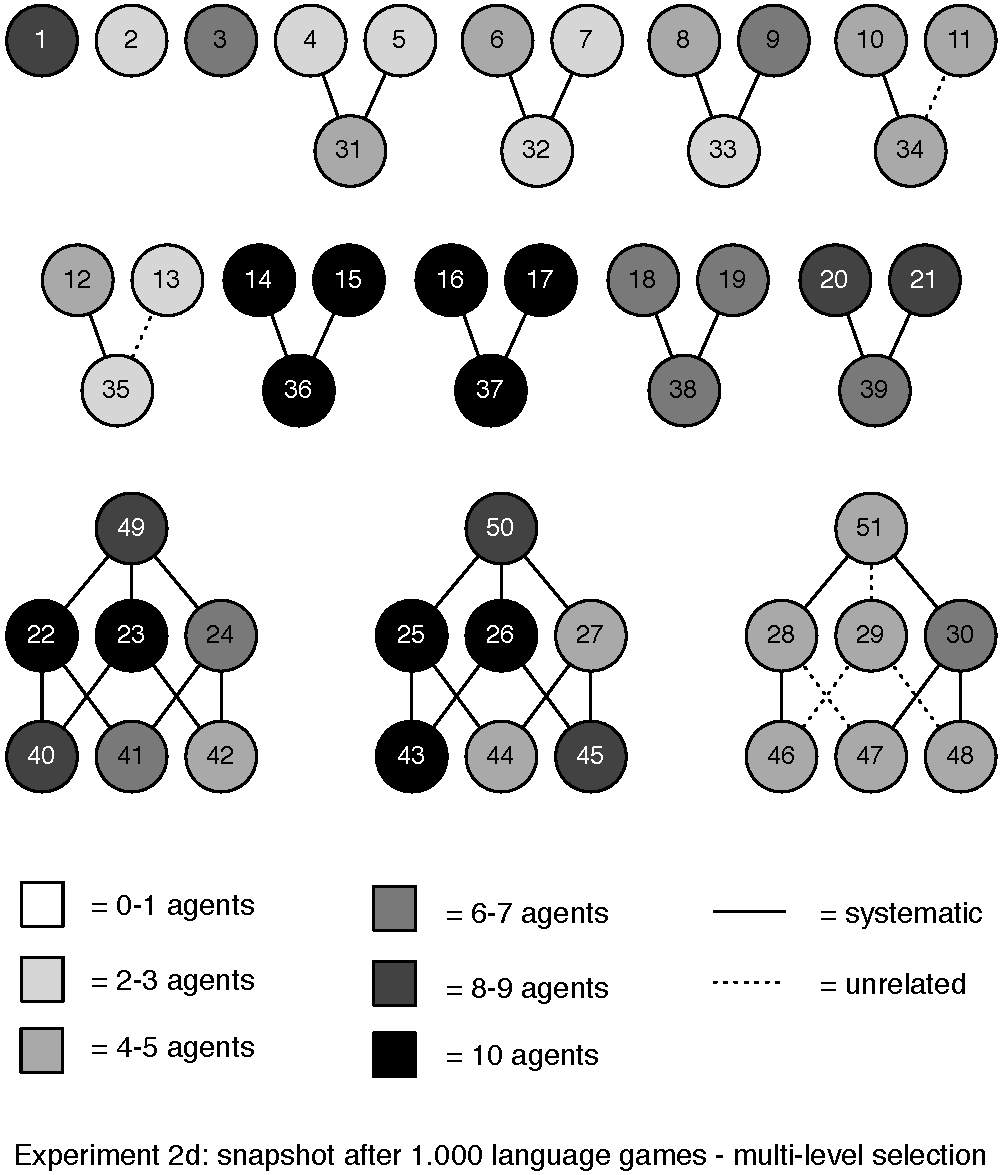
\includegraphics[width=0.7\textwidth]{Chapter4/figs/multilevel-coherence-no-analogy-1000}}
  \caption[Experiment 2: snapshot after 1.000 games (multi-level selection\is{multi-level selection})]{This diagram gives a snapshot of the average coherence in a population\is{speech population} of 10 agents after 1.000 language game\is{language game}s using the multi-level selection\is{multi-level selection} alignment strateg\is{alignment strategy}y. Compared to the simulations using direct selection, the agents seem to be converging more rapidly on meaning-form mappings and have already settled on 11 of them. Whereas there was no convergence at all yet for the more complex meanings 49--51 in the simulations using the direct selection alignment strateg\is{alignment strategy}y, here they are already shared by a majority of the population\is{speech population}. This suggests that multi-level selection\is{multi-level selection} speeds up the convergence dynamics significantly especially for related meanings. For the meanings in the bottom right, there is less systematicity\is{systematicity} and hence convergence takes longer time.}
   \label{f:2d-coherence-1000}
\end{figure}
\begin{figure}[p]
\centerline{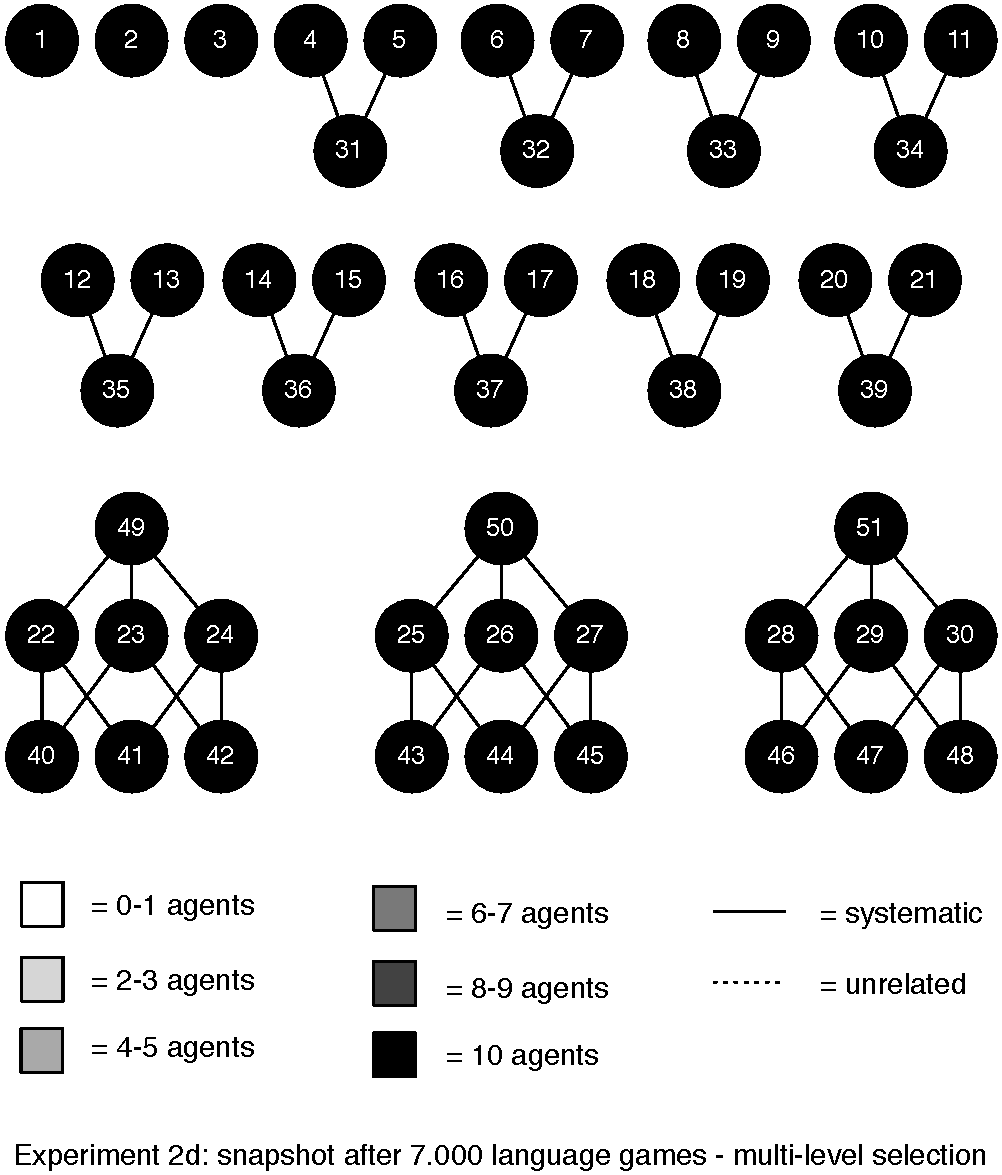
\includegraphics[width=0.7\textwidth]{Chapter4/figs/multilevel-coherence-no-analogy-7000}}
  \caption[Experiment 2: snapshot after 7.000 games (multi-level selection\is{multi-level selection})]{This diagram gives a snapshot of the average coherence in a population\is{speech population} of 10 agents after 7.000 language game\is{language game}s using the multi-level selection\is{multi-level selection} alignment strateg\is{alignment strategy}y. All the circles are black which means that the entire population\is{speech population} prefers the same meaning-form mappings. The language is also fully systematic so the agents have converged on 30 case marker\is{case!case marking}s which can be combined into 51 different constructions. The results indicate that even for instance-based\is{exemplar-based models} learners/innovat\is{innovation}ors systematicity\is{systematicity} can be reached by keeping a link between newly acquired constructions and the constructions that were used for learning or creating them.}
   \label{f:2d-coherence-7000}
\end{figure}
\\
\\
\noindent{\bfseries Discussion.} The results show that the agents reach full systematicity\is{systematicity} if each level in the linguistic inventor\is{linguistic inventory}y can have an influence on the competit\is{competition}ion in other levels. It is now important to understand why this is the case and why the other alignment strateg\is{alignment strategy}ies did not yield full systematicity\is{systematicity}.

First of all, bottom-up selection doesn't improve on the results of experiment 1 in terms of convergence speed and it doesn't lead to a systematic mapping of meaning to form across patterns. A closer examination of the the alignment strateg\is{alignment strategy}y reveals that the relatively high systematicity\is{systematicity} of 80\% is due to the higher frequency\is{frequency} of single-argument constructions. The frequent use of these constructions each time has repercussions for the competit\is{competition}ion between larger constructions whereas this is not the case in the other direction. If there would be more patterns than single-argument constructions, the improvement would therefore be less high. The patterns that resist the bottom-up selection can do so because the competit\is{competition}ion is not fully decided yet on a lower level (each time reinforc\is{reinforcement}ing competing patterns) and there is additional competit\is{competition}ion on the level of the patterns themselves which may have different winners than those on lower levels. In the end, though, the bottom-up strategy should lead to full systematicity\is{systematicity} but only very slowly and because the smaller constructions are more frequent.

The top-down strategy is affected by frequency\is{frequency} as well: competit\is{competition}ion between the larger constructions has significant impact on lower levels because it can increase the scores of up to six constructions while at the same time punishing all competit\is{competition}ors. However, since the smaller constructions are actually more frequent than the larger ones, some divergent competit\is{competition}ion pathways may resist this influence from the patterns and survive nevertheless. As the results indicate, this in fact happens in most of the simulations. Top-down selection thus improves systematicity\is{systematicity} significantly, but it is affected by the frequency\is{frequency} of the various levels of linguistic items and it is therefore no guarantee of full systematicity\is{systematicity}.

Finally, the agents can achieve full systematicity\is{systematicity} through multi-level selection\is{multi-level selection}. This strategy allows the competit\is{competition}ion of each level to influence the competit\is{competition}ion on others and given its n-directionality, it is not (or less) dependent on differences in frequency\is{frequency}. Moreover, the agents do not need to differentiate between a `higher' and a `lower' level but can treat all links between constructions on equal footing. The results of experiment 2 confirm earlier results on multi-level selection\is{multi-level selection} and systematicity\is{systematicity} reported by \citet{steels07multilevel}. In these experiments, which involved a scale-up in convergence space, multi-level selection\is{multi-level selection} outperforms the other strategies even more significantly.

\section{Experiment 3: multi-level selection\is{multi-level selection} with analog\is{analogy}y}
\label{s:pattern-exp-3}

Similarly to the previous experiments, experiment 3 investigates how baseline experiment 3 can be extended with a diagnostic\is{learning strategies!diagnostics} and repair\is{learning strategies!repair strategies} for pattern formation\is{formation}\is{pattern formation}. Since the previous experiments identified the problem of systematicity\is{systematicity}, experiment 3 first of all needs to verify whether the conclusions of the second experiment also hold for the new set-up in which the agents are capable of performing analog\is{analogy}ical reasoning over events. I will then report an experiment that adapts the algorithm for multi-level selection\is{multi-level selection} to the token-frequency\is{frequency} alignment strateg\is{alignment strategy}y of baseline experiment 3d (see section \ref{s:base3}).

\subsection{Experimental set-up}

Experiment 3 features the same experimental set-up as baseline experiment 3 with the addition of a diagnostic\is{learning strategies!diagnostics} and repair\is{learning strategies!repair strategies} strategy for pattern formation\is{formation}\is{pattern formation}. To summarize:

\begin{itemize}
\item The population\is{speech population} consists of 10 agents that engage in description game\is{language game!description game}s;
\item The meaning space is the same one as detailed in Table \ref{t:events} and all event type\is{event type}s occur with the same frequency\is{frequency};
\item The agents have two diagnostic\is{learning strategies!diagnostics}s: detecting unexpressed variable equal\is{variable equality}ities and the new diagnostic\is{learning strategies!diagnostics} detecting whether two constructions were applied during processing;
\item The agents have two repair\is{learning strategies!repair strategies} strategies: one for inventing and learning new verb\is{verb}-specific marker\is{case!case marking}\is{case!case marking}s and one for combining these marker\is{case!case marking}\is{case!case marking}s into a larger construction. The invention and learning strategy also includes the possibility of exten\is{extension}ding and reusing\is{reuse} existing marker\is{case!case marking}\is{case!case marking}s through analog\is{analogy}ical reasoning. The algorithm for analog\is{analogy}y is the same as in baseline experiment 3 and only looks at individual marker\is{case!case marking}\is{case!case marking}s.
\end{itemize}

The experiment has been tested using five different alignment strateg\is{alignment strategy}ies. The first four strategies are individual selection, top-down selection, bottom-up selection and multi-level selection\is{multi-level selection} using the same fine-grained lateral inhibition\is{lateral inhibition} mechanism as used in baseline experiment 3c. This means that competit\is{competition}ion is only held at the level of the co-occur\is{co-occurrence}rence links between a construction and a lexical entry rather than at the level of the constructions themselves. The algorithms can be summarized as follows:

\begin{itemize}
\item {\bfseries Individual selection:} This is the exact same set-up as baseline experiment 3c. If a game was successful, the hearer will increase the score of the co-occur\is{co-occurrence}rence link between the applied lexical entry and the applied construction(s) by 0.1. He will also decrease the scores of the competing links by 0.1. The score of a link is always between 0 (high uncertainty) and 1 (high confidence\is{confidence}).
\item {\bfseries Top-down selection:} In this strategy, the hearer will not only increase the score of the relevant co-occur\is{co-occurrence}rence link, but also the score of all the co-occur\is{co-occurrence}rence links that link the lexical entry to the smaller constructions which are related to the applied construction. The scores of the competit\is{competition}ors of these links are decreased.
\item {\bfseries Bottom-up selection:}  In this strategy, the hearer increases the score of the relevant link and of all the co-occur\is{co-occurrence}rence links that link the lexical entry to the larger constructions which are related to the applied constructions. All competit\is{competition}ors of these links are punished.
\item {\bfseries Multi-level selection\is{multi-level selection}:} In this strategy, the hearer increases the scores of the relevant co-occur\is{co-occurrence}rence links and of all the links which link the lexical entry to constructions that are related to the applied constructions.
\end{itemize}

The fifth experimental set-up does not involve lateral inhibition\is{lateral inhibition} but implements {\bfseries multi-level selection\is{multi-level selection} and memory decay\is{memory decay}}. In this set-up, the hearer will not only increase the frequency\is{frequency} score of the applied constructions, but also that of all the related constructions by 1. The frequency\is{frequency} scores have no upper limit, so the higher the score, the more entrench\is{entrenchment}ed the construction is. After an agent has individually engaged in 200 language game\is{language game}s, the frequency\is{frequency} scores of all the items in the inventory are decreased.

In all five set-ups, the speaker will use the co-occur\is{co-occurrence}rence links to speed up processing. This means that not the entire inventory of constructions is considered, but only those constructions which are linked to the lexical entry. Links can be added through co-occur\is{co-occurrence}rence. When the speaker is faced with multiple hypotheses, he will choose the construction which either has the strongest co-occur\is{co-occurrence}rence link with the lexical entry (in the first four set-ups) or the one with the highest token frequency\is{token frequency}\is{frequency} (in the fifth set-up). During processing, only the scores of individual competit\is{competition}ors are taken into account. All simulations have been run in 10 series of 12.000 language game\is{language game}s.

\subsection{Results and discussion}

In this section, the first four set-ups are again compared to each other to demonstrate the reoccurrence of the problem of systematicity\is{systematicity}. The fourth set-up (multi-level selection\is{multi-level selection} with lateral inhibition\is{lateral inhibition}) is then compared more thoroughly to the fifth set-up using multi-level selection\is{multi-level selection} and memory decay\is{memory decay}. Finally, this section offers a closer look at one language evolved using the fifth set-up.
\begin{figure}[p]
\centerline{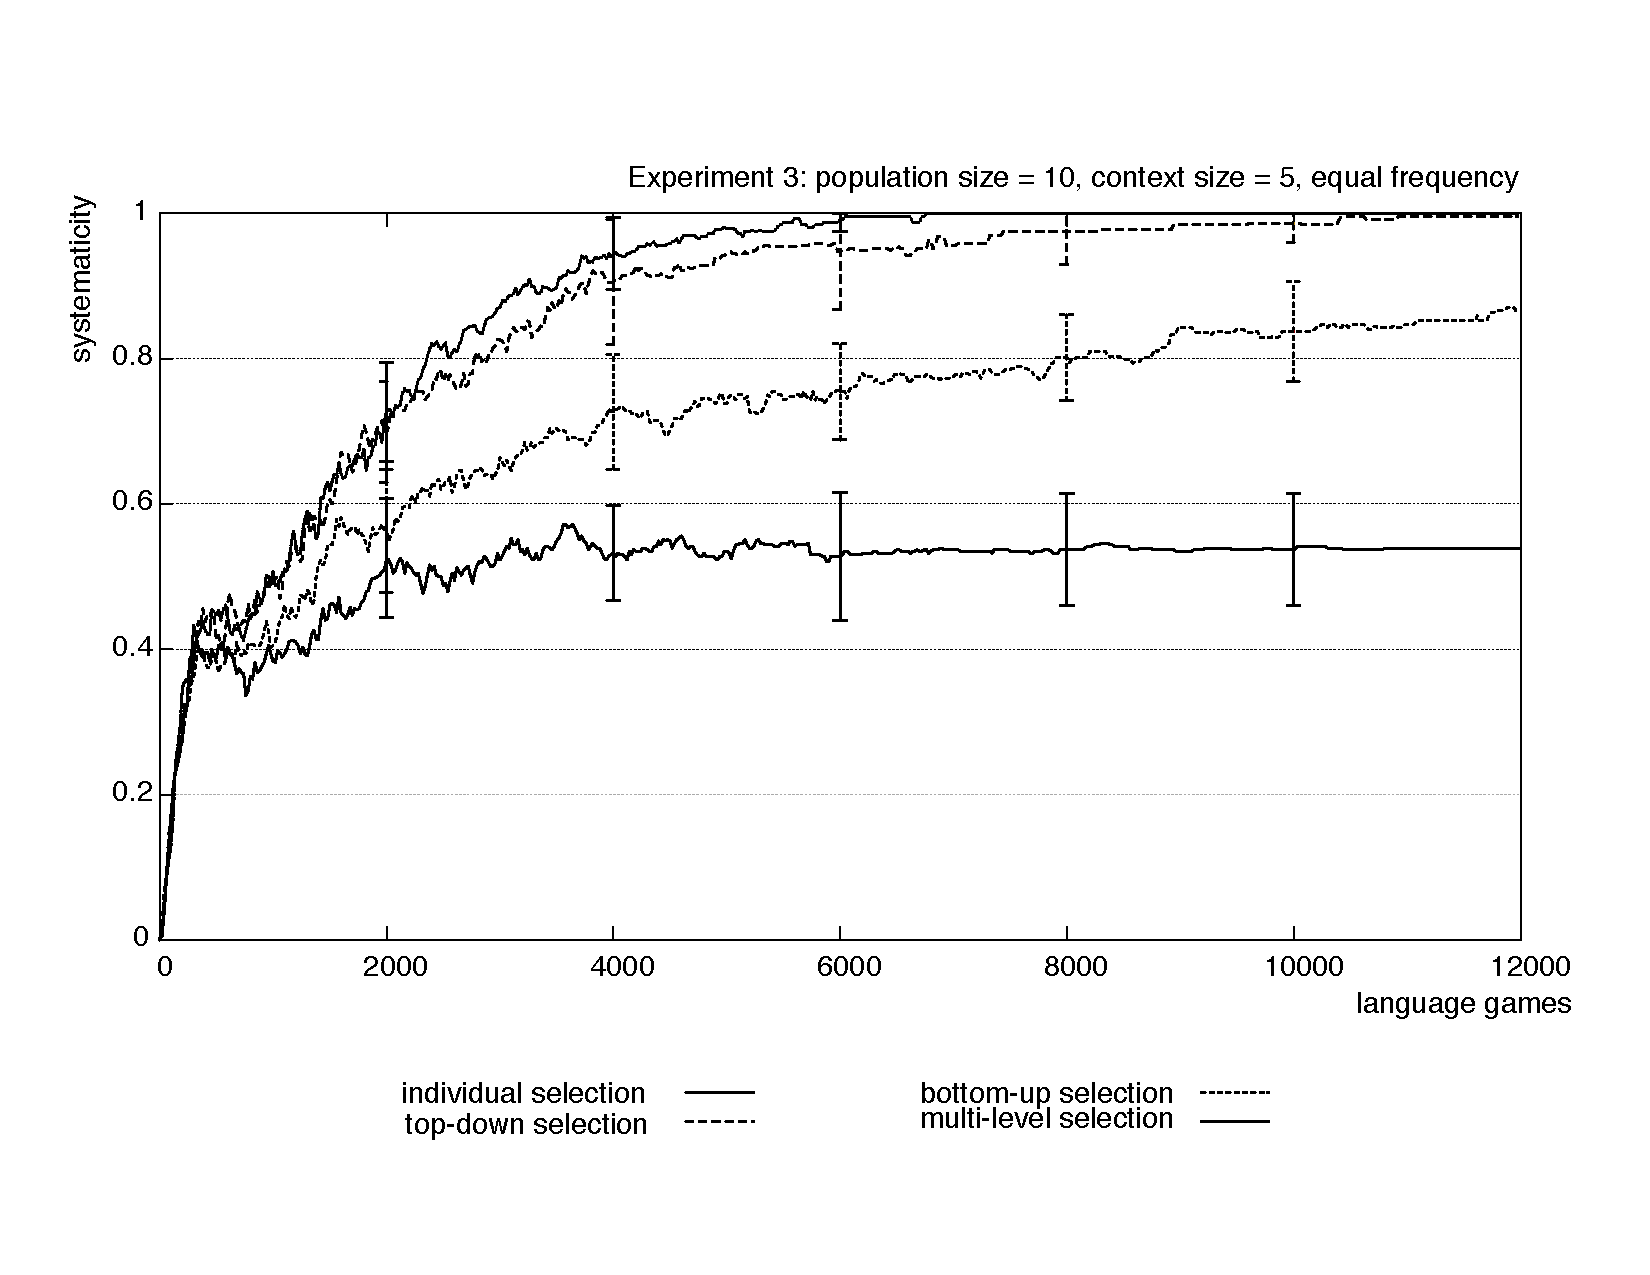
\includegraphics[width=\textwidth]{Chapter4/figs/systematicity3}}
  \caption[Experiment 3: systematicity]{This graph compares systematicity\is{systematicity} in the first four experimental set-ups of experiment 3. The results confirm those of experiment 2. Even though there is potentially less variation\is{variation} because of the reuse\is{reuse} of existing marker\is{case!case marking}s, individual selection stagnates at 50\% systematicity\is{systematicity}. Bottom-up selection increases systematicity\is{systematicity} beyond 80\% but also gets stuck. Top-down selection manages to reach full systematicity\is{systematicity} in more simulations than in experiment 2 because of the smaller variation\is{variation} space, but does not guarantee full systematicity\is{systematicity}. Only multi-level selection\is{multi-level selection} reaches systematicity\is{systematicity} in all the simulations and does so significantly faster than the other alignment strateg\is{alignment strategy}ies.}
   \label{f:systematicity3}
\end{figure}
\\
\\
\noindent{\bfseries Results.} Figure \ref{f:systematicity3} compares the first four experimental set-ups to each other in terms of systematicity\is{systematicity}. The lines indicating systematicity\is{systematicity} for each set-up show the same behaviour as those in experiment 2 (Figure \ref{f:systematicity2}). The first set-up using the alignment strateg\is{alignment strategy}y of individual selection fluctuates between 45 and 60\% systematicity\is{systematicity} and stops evolving after 6.000 language game\is{language game}s. The bottom-up strategy reaches more than 80\% systematicity\is{systematicity} after 8.000 language game\is{language game}s. In some simulations, this strategy leads up to 90\% but never to maximum systematicity\is{systematicity}. Top-down selection performs a bit better than in experiment 2 due to the fact that the agent's capacity of reusing\is{reuse} existing marker\is{case!case marking}s leads to a smaller variation\is{variation} space so `frozen accidents' are less likely. Yet, as the results show, some simulations still involve an unsystematic convention\is{convention} and reaching systematicity\is{systematicity} takes a longer time than the multi-level selection\is{multi-level selection} strategy. The latter strategy is again the only one which leads to full systematicity\is{systematicity} in all the simulations.
\begin{figure}[p]
\centerline{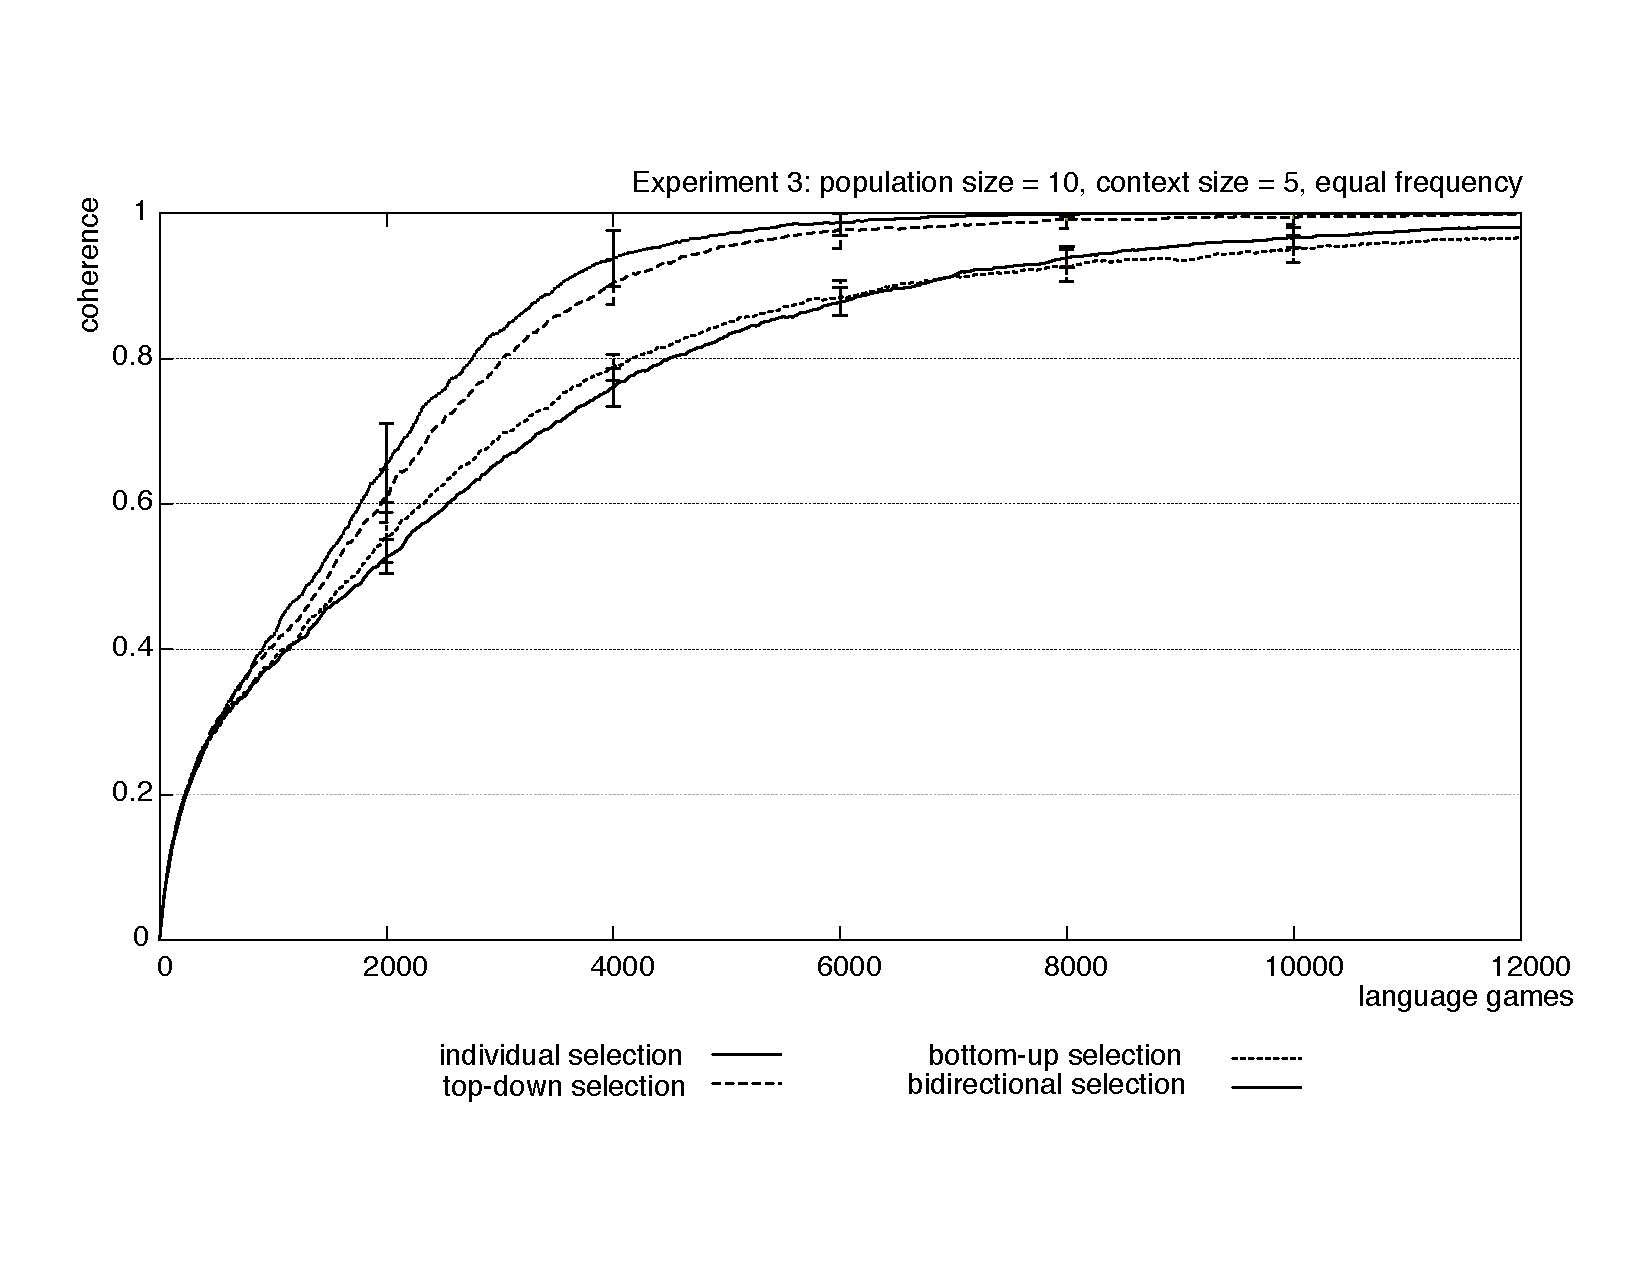
\includegraphics[width=\textwidth]{Chapter4/figs/coherence3}}
  \caption[Experiment 3: coherence]{This graph compares the first four set-ups of experiment 3 in terms of meaning-form coherence. The graph shows that multi-level and top-down selection perform equally well and reach 100\% between 6.000 and 8.000 language game\is{language game}s. Bottom-up and individual selection again run almost parallel and reach coherence faster than in experiment 2 because of the smaller variation\is{variation} space.}
   \label{f:coherence3}
\end{figure}

The four set-ups also confirm the results of experiment 2 in terms of coherence. Figure \ref{f:coherence3} shows that bottom-up selection and individual selection again run almost parallel in terms of convergence. This time the agents reach coherence faster because of the smaller variation\is{variation} space. Multi-level and top-down selection also perform equally well and reach coherence between 6.000 and 8.000 language game\is{language game}s.
\begin{figure}[t]
\centerline{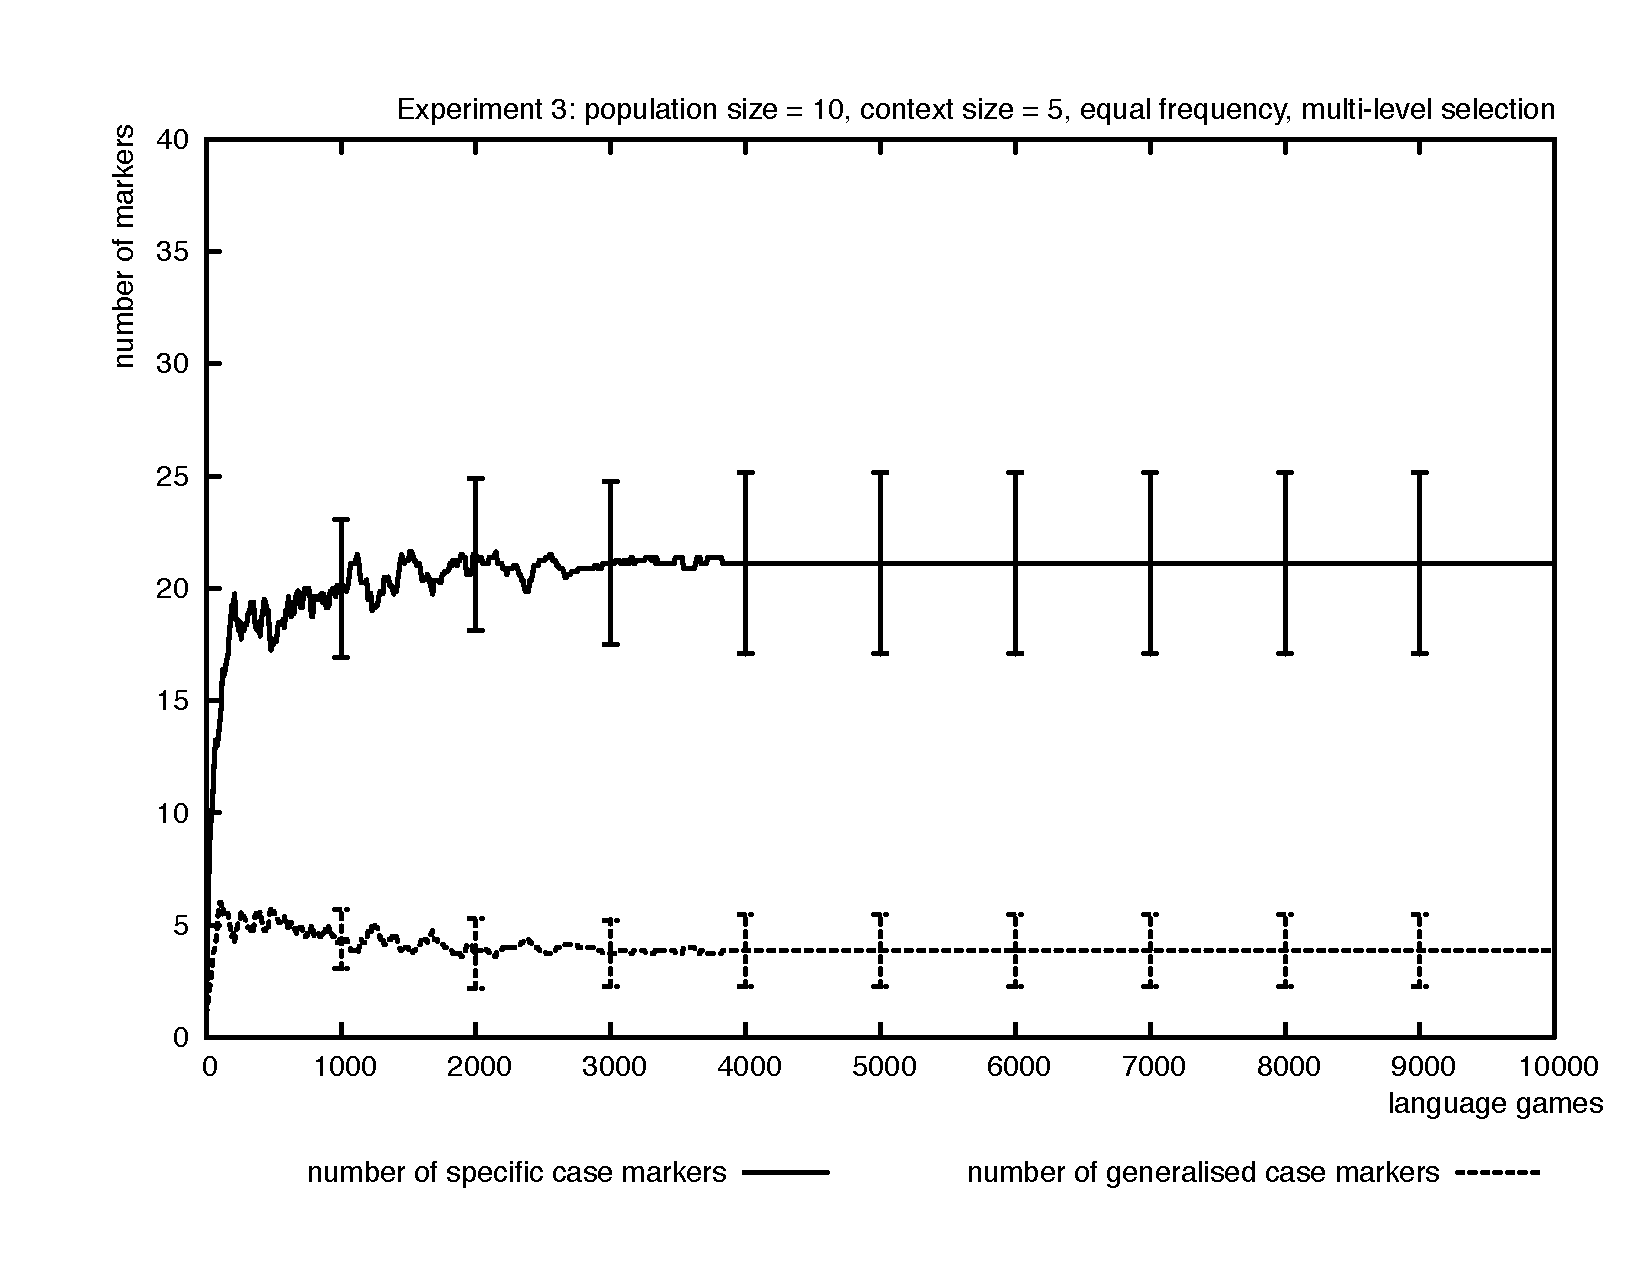
\includegraphics[width=\textwidth]{Chapter4/figs/markers3}}
  \caption[Experiment 3: number of markers]{This graph shows the average number of marker\is{case!case marking}s known by each agent using the strategy of multi-level selection\is{multi-level selection} with lateral inhibition\is{lateral inhibition} (the fourth set-up of experiment 3). The results show that the generalization rate of the agents is not impressive: only 3-5 semantic roles survive the competit\is{competition}ion as opposed to 18-25 specific marker\is{case!case marking}s.}
   \label{f:markers3}
\end{figure}

Figure \ref{f:markers3} gives an indication of the kinds of languages that are formed in the population\is{speech population} if the agents use the fourth set-up (multi-level selection\is{multi-level selection} with lateral inhibition\is{lateral inhibition}). The graph shows that the generalization rate of the agents is not really impressive: only three to five generaliz\is{generalization}ed roles survive the competit\is{competition}ion. Moreover, these roles only cover two or maximally three participant roles. This is clear from the fact that there are still 18 to 25 specific marker\is{case!case marking}s floating around in the population\is{speech population}.
\begin{figure}[p]
\centering
\begin{tabular}{c}
{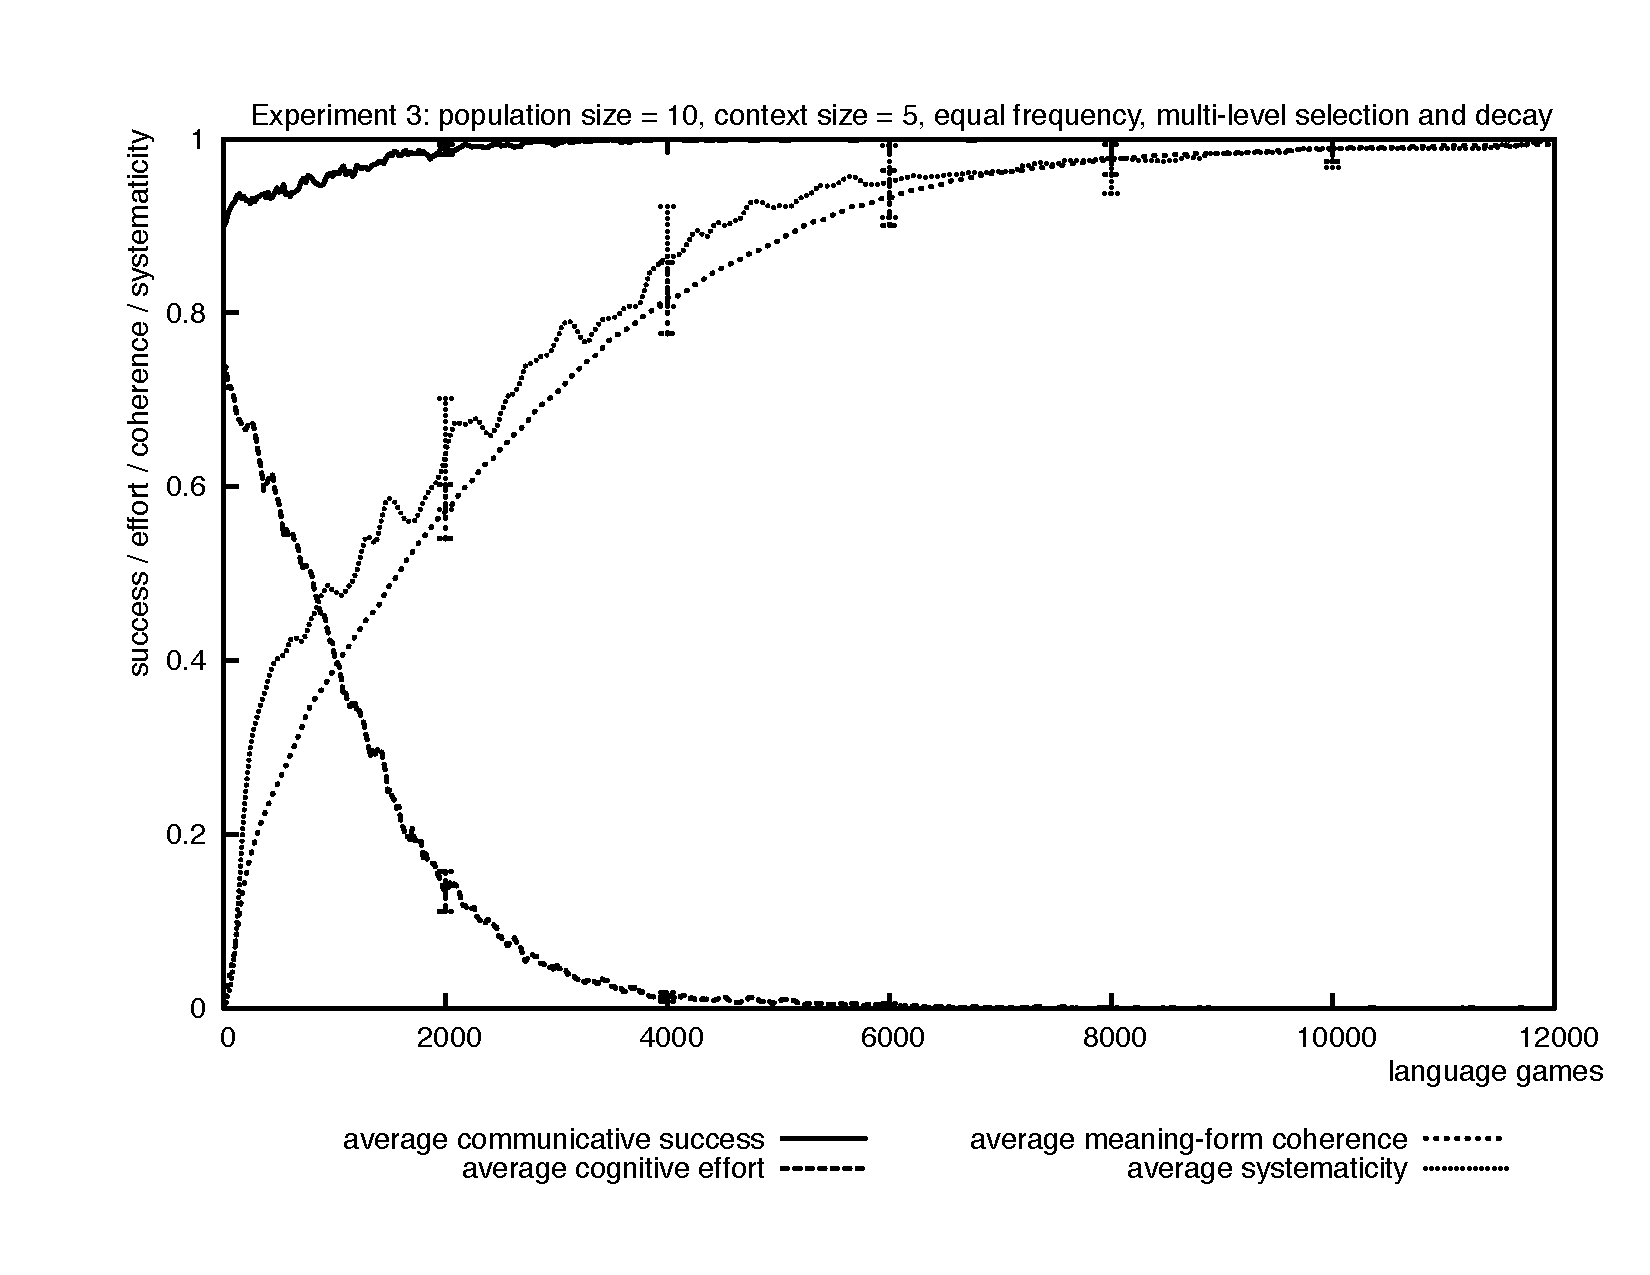
\includegraphics[width=0.8\textwidth]{Chapter4/figs/systematicity3b}}
\\
{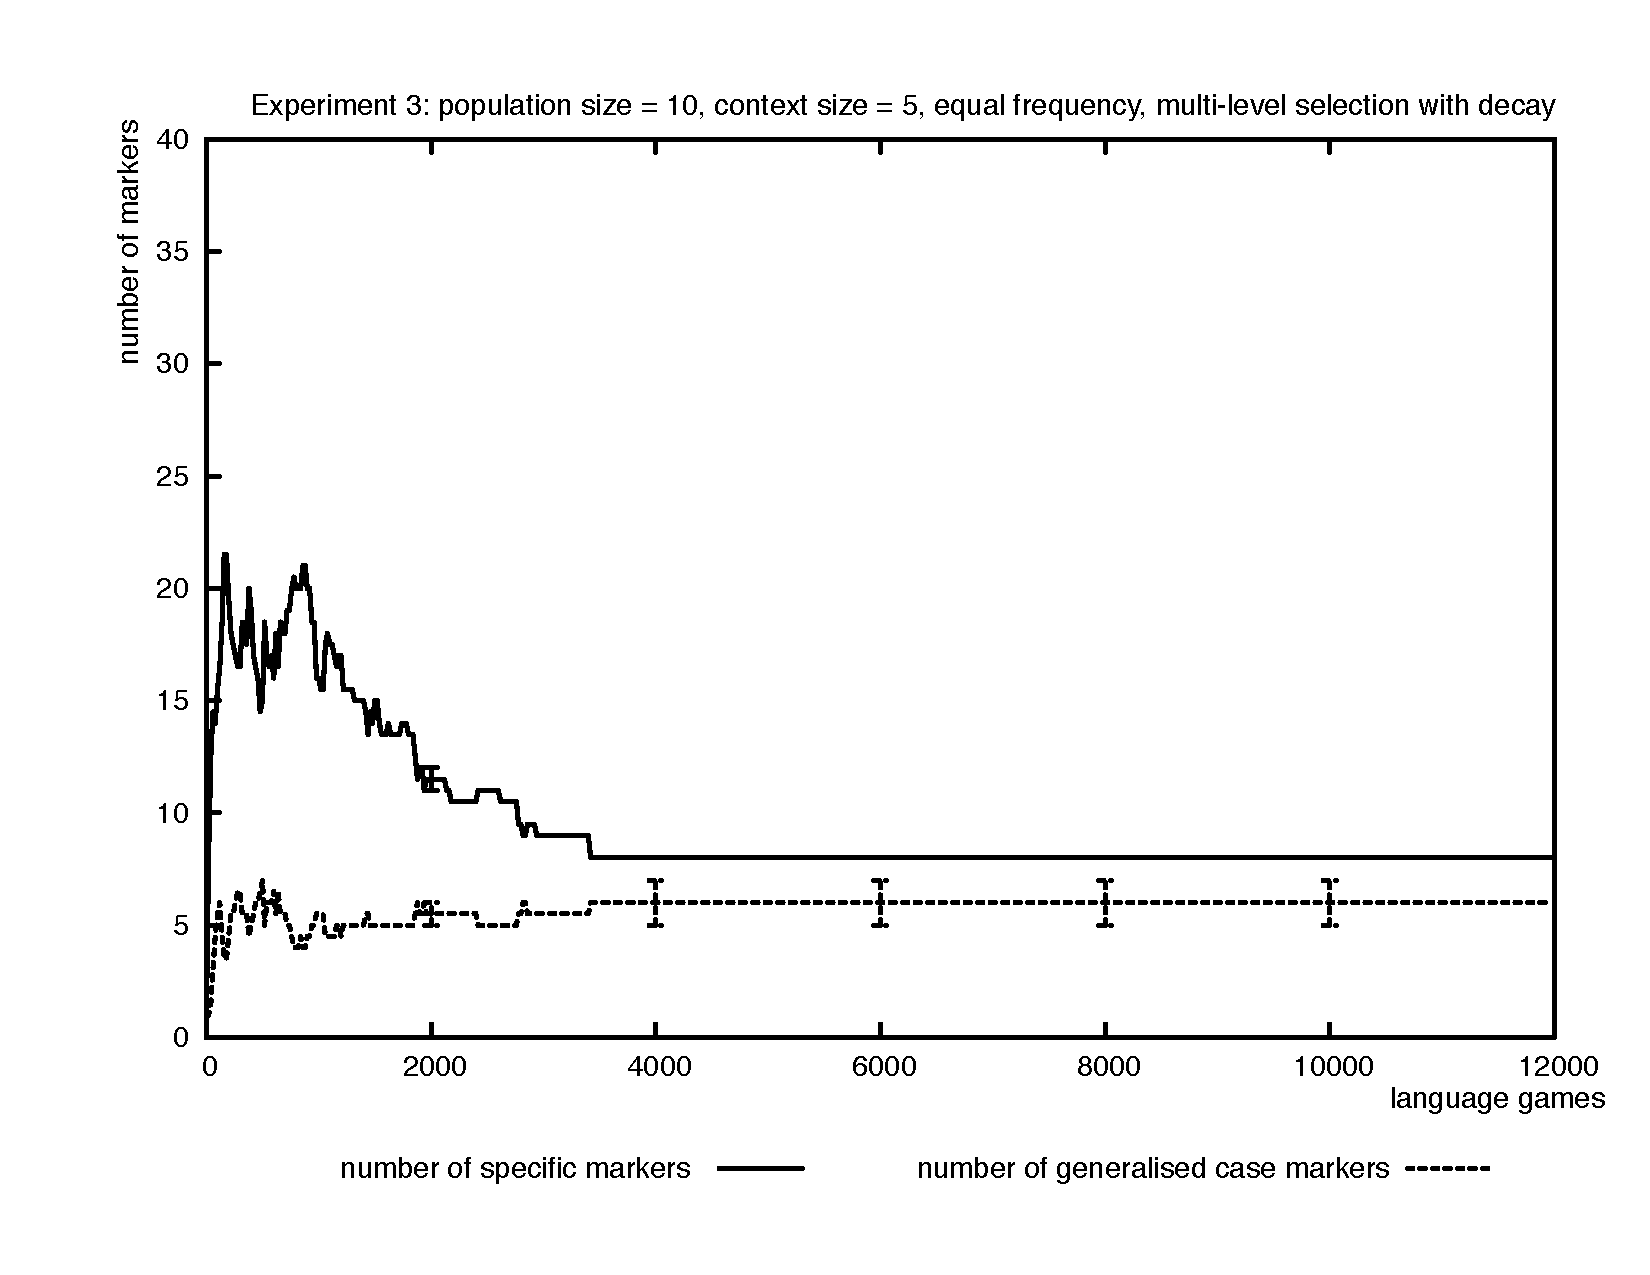
\includegraphics[width=0.8\textwidth]{Chapter4/figs/markers3-decay}}
\end{tabular}
\caption[Experiment 3: results for set-up 4]{The top graph shows communicative success\is{communicative success}, cognitive effort\is{cognitive effort}, systematicity\is{systematicity} and meaning-form coherence in the set-up using multi-level selection\is{multi-level selection} and decay. The bottom graph shows the average number of marker\is{case!case marking}s in the same set-up.}
\label{f:multi-level-decay}
\end{figure}

These results can be compared to the performance\is{performance} of the fifth set-up (multi-level selection\is{multi-level selection} with decay) which is illustrated in Figure \ref{f:multi-level-decay}. The top graph shows the results for communicative success\is{communicative success}, cognitive effort\is{cognitive effort}, meaning-form coherence and systematicity\is{systematicity}. As the graph indicates, the agents succeed in reaching full systematicity\is{systematicity} somewhere between 8.000 and 12.000 language game\is{language game}s, which is a bit slower than the alignment strateg\is{alignment strategy}y using lateral inhibition\is{lateral inhibition}. The bottom graph shows the average number of marker\is{case!case marking}s floating around in the population\is{speech population}. Here, we see that the average number of specific marker\is{case!case marking}s has made a significant drop from 18-25 marker\is{case!case marking}s to only 9. The number of semantic roles shifts from simulation to simulation between 4 and 6. The semantic roles also tend to be more general categories than in the simulations using lateral inhibition\is{lateral inhibition}.
\\
\\
Here is a list of marker\is{case!case marking}s and the participant roles they cover in one of the simulations (from more general to more specific):

\begin{itemize}
\item {\em -kad:} object-1, approach-1, fall-1, touch-1, move-outside-1
\item {\em -fuir:}  grasp-2, hide-2, move-inside-2, touch-2, walk-to-1
\item {\em -kazo:} approach-2, fall-2, grasp-1, hide-1, walk-to-2
\item {\em -hesa:} move-1, take-3
\item {\em -ti:} visible-1, take-1
\item {\em -qiwo:} move-inside-1, give-3
\item {\em -fen:} distance-decreasing-1
\item {\em -rem:} distance-decreasing-2
\item {\em -gaeh:} move-outside-2
\item {\em -wupu:} cause-move-on-1
\item {\em -chuiw:} cause-move-on-2
\item {\em -nuip:} cause-move-on-3
\item {\em -tu:} give-1
\item {\em -hozae:} give-2
\item {\em -fut:} take-2
\end{itemize}

The above marker\is{case!case marking}s occur systematically across patterns for marking the same parti\-ci\-pant roles. In this specific example, the agents succeeded in reaching coherence and systematicity\is{systematicity} after only 8.000 language game\is{language game}s. When we compare the results to those of baseline experiment 3d, roughly the same level of generalization is reached.

\begin{figure}[p]
\centerline{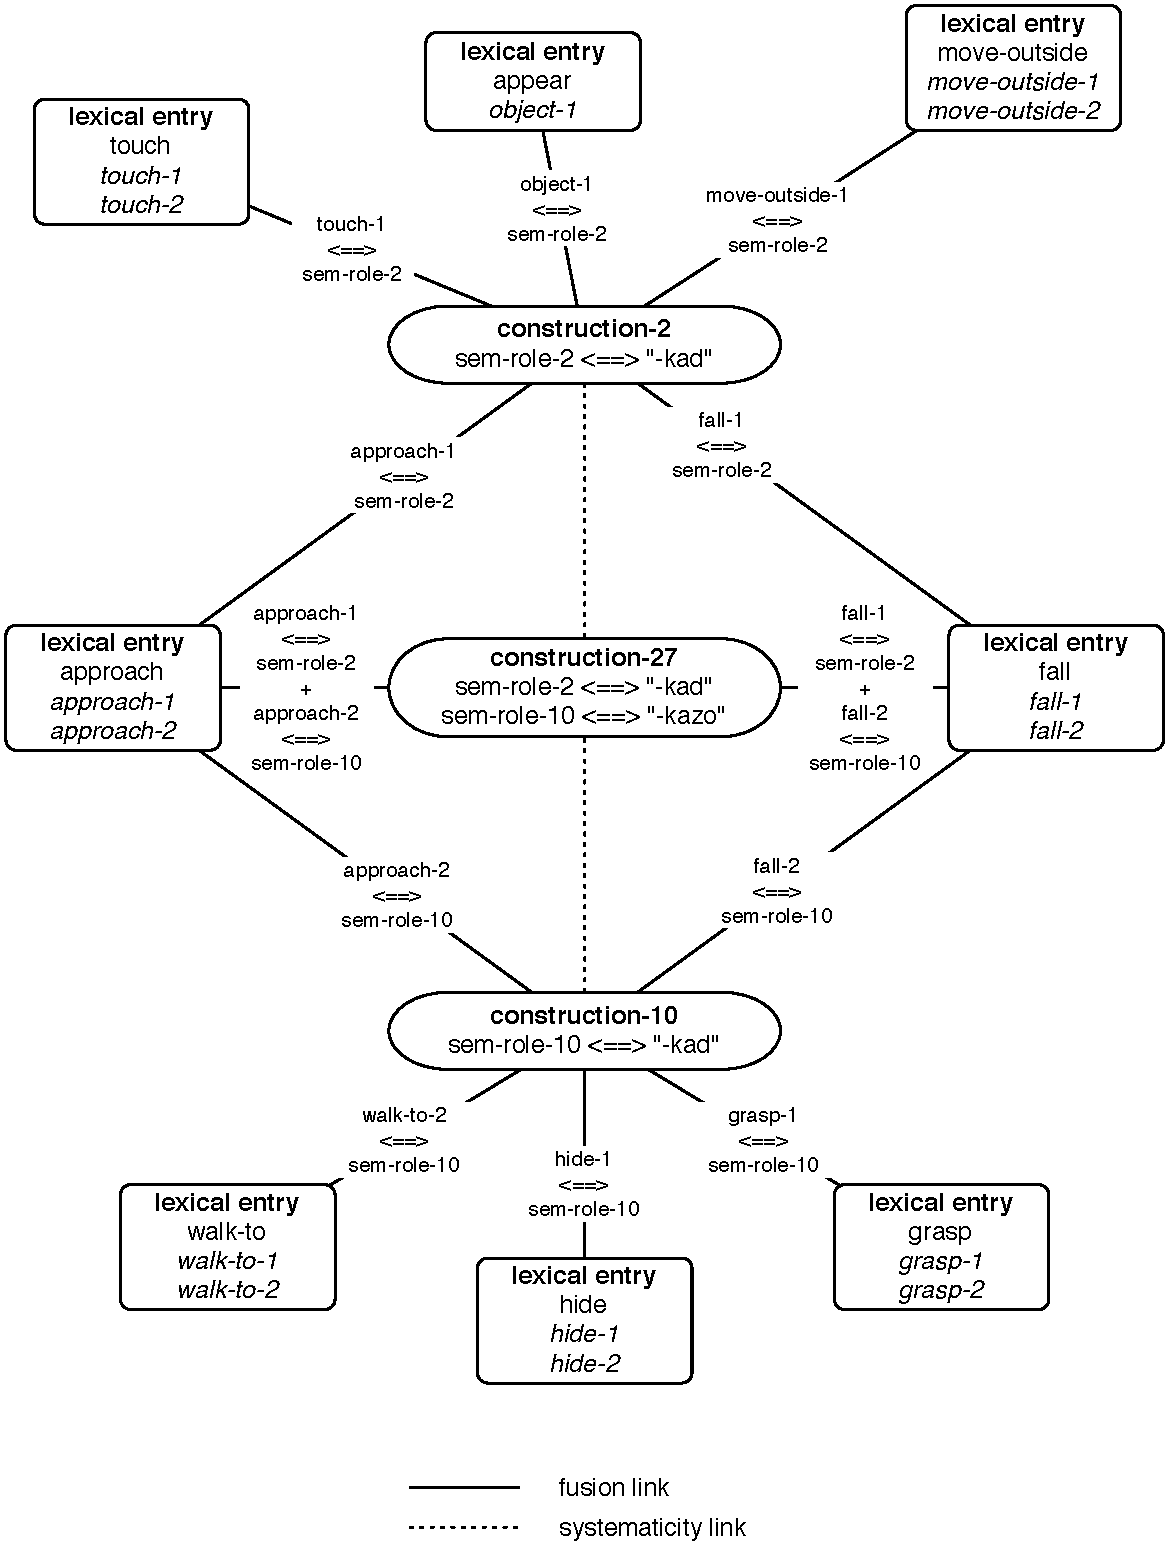
\includegraphics[width=0.75\textwidth]{Chapter4/figs/network}}
  \caption[Experiment 3: a partial network of set-up 5]{This figure gives a partial network for one agent in one of the simulations using multi-level selection\is{multi-level selection} with decay. In the middle there are three constructions which are systematically related to each other. The constructions are also linked with lexical entries. The links act both as co-occur\is{co-occurrence}rence links for optimizing processing and as fusion\is{fusion} links for integrating the participant roles of the lexical entries with the semantic roles of the constructions. The networks are constructed in a stepwise fashion as a response to communicative needs.}
   \label{f:network}
\end{figure}

Finally, Figure \ref{f:network} looks inside the linguistic inventor\is{linguistic inventory}y of a single agent and offers a partial network of the agent's knowledge of its language. The figure concentrates on three constructions (in the middle) which are related to each other (indicated by the dotted line). The relation between the constructions indicate that construction-27 was created as a pattern of construction-2 and construction-10. The figure also shows all the lexical entries that are convention\is{convention}ally associated with these constructions. The links between the lexical entries and the constructions are used for optimizing processing: instead of trying out all the constructions in memory, only the linked constructions are considered. Links can be added as part of a problem-solving\is{problem-solving} process during communication or pruned if the co-occur\is{co-occurrence}rence is not a successful one. Some redundant co-occur\is{co-occurrence}rence links may survive in the inventory. The links can also be seen as fusion\is{fusion} links: they are annotated with information on how the participant roles can be fused with the semantic roles of the construction. This annotation is however not used by the agents themselves but for the clarity of interpretation for the experimenter. The actual fusion\is{fusion} is taken care of by the unification\is{unification} of the potential valents of the lexical entry with the actual valency of the construction.
\\
\\
\noindent{\bfseries Discussion.} The results of experiment 3 confirm the problem of systematicity\is{systematicity} that was uncovered in the other experiments. Here too, the strategy using multi-level selection\is{multi-level selection} was the only one to yield fully systematic languages. The systematicity\is{systematicity} rate was in each of the first four set-ups comparable to the rates in experiment 2. This may come as a surprise since the variation\is{variation} space is potentially smaller because the agents can exten\is{extension}d the use of existing marker\is{case!case marking}s rather than inventing new ones all the time.

A closer look at the number of marker\is{case!case marking}s in the fourth set-up (multi-level selection\is{multi-level selection} with lateral inhibition\is{lateral inhibition}), however, pointed to the reason for the small differences in systematicity\is{systematicity} rates: only a very small number of semantic roles survived the competit\is{competition}ion compared to a large number of specific marker\is{case!case marking}s. This means that the generalization rate is not really impressive so the number of variation\is{variation}s is not much smaller in these simulations than was the case in experiment 2. The resulting number of specific mar\-kers versus semantic roles corresponds to the results obtained in baseline experiment 3c and also the reason for the result is the same: since the competit\is{competition}ion is held at the level of co-occur\is{co-occurrence}rence links and not at the level of constructions, the type frequency\is{type frequency}\is{frequency} of a marker\is{case!case marking} does not translate into a larger category gravity\is{category gravity}. Competition is held only in a local context so specific mar\-kers have an equally high chance of winning as more generaliz\is{generalization}ed semantic roles.

The results of the fifth set-up (multi-level selection\is{multi-level selection} with memory decay\is{memory decay}) also confirm the results of the baseline experiments and improve significantly in terms of generalization over the simulations using the fine-grained lateral inhibition\is{lateral inhibition} dynamics. The number of specific categories has dropped by half and larger, more general semantic roles have a selectionist advantage because they occur more often. The generalization rate roughly matches the performance\is{performance} of baseline experiment 3d.

The consistency in number of generaliz\is{generalization}ed semantic roles and specific marker\is{case!case marking}s across the baseline experiments and the pattern experiments indicate that this is the maximum generalization rate that the agents can reach. Possible improvements would have to come from two sources:

\begin{enumerate}
\item The structure of the world: The capacity of analog\is{analogy}ical reasoning is heavily dependent on the structure of the world environment in which communication takes place. If the agents have to communicate about lots of events which show recurrent patterns in terms of visual primitives, they will be able to detect more analog\is{analogy}ies. If, however, the world is totally unstructured, the agents will come up with more specific marker\is{case!case marking}s than general semantic roles.
\item The capacity of analog\is{analogy}ical reasoning can be made more flexible. At the moment, the agents make a sharp distinction between what is analog\is{analogy}ous and what is not. A possible relaxation could be to only care about whether the mapping between a source\is{semantic role!source} role and a target role is discriminating enough for identifying the target role as well. Another possibility would be to use a similarity or a distance metric instead of the more rigid structural mapping that the agents currently use.
\end{enumerate}

Experiment 3 also shows the potential power of the combination of analog\is{analogy}ical reasoning, pattern formation\is{pattern formation} and multi-level selection\is{multi-level selection} respectively. First of all, analog\is{analogy}ical reasoning over the linguistic inventor\is{linguistic inventory}y can lead to an increasing generalization rate in the population\is{speech population}, as is also shown in several instance-based\is{exemplar-based models} approaches to language \citep{daelemans05memory, skousen89analogical}. These models also argue that a language can look rule-based from outside whereas in fact the generalization is distributed over the linguistic items in the inventory. This experiment shows that this observation also holds true for the case of the emergence\is{emergence} of grammar if multi-level selection\is{multi-level selection} is applied. Finally, the formation\is{formation} of patterns to improve processing can have dramatic effects on the grammar: the patterns increase the survival chances of its related items; and they may potentially exten\is{extension}d their use as well in later interactions. 

So far, I did not spend much attention to the efficiency of the formalization of argument realization proposed in Chapter \ref{c:ar}. In all the experiments presented in this Chapter and the previous one, the representation has proven to be flexible enough to deal with the enormous amount of {\bfseries uncertainty} that is inherent to the emergence\is{emergence} of new grammar convention\is{convention}s. In this case, the agents needed a flexible way of integrating lexical entries with constructions of various degrees of entrench\is{entrenchment}ment. Instead of copying all the possible case frames into a new entry, the formalization allowed the agents to constantly `mould' their lexical entries until a stable set of convention\is{convention}s had been negotiat\is{negotiation}ed. In this way, the competit\is{competition}ion of case marker\is{case!case marking}s could be held exclusively at the level of constructions instead of creating an additional competit\is{competition}ion on the lexical level for how these lexical entries should be integrated with the constructions. The lexical entries also integrated as easily with verb\is{verb}-specific construction\is{construction!verb-specific construction}s as with verb\is{verb}-class specific constructions.

The formalization was also flexible enough to deal with {\bfseries multiple argument realization}: the agents were capable of integrating a single lexical entry into multiple patterns or constructions without the need for deriv\is{derivation}ational rules or additional copies in the lexicon\is{lexicon}. Moreover, the lexical entries do not need to `profile' their participant roles: the actual valency of a verb\is{verb} is determined by the construction it integrates with. Preferences for certain patterns of argument realization could be captured in this formalization by assigning a frequency\is{frequency} score to the co-occur\is{co-occurrence}rence links of the lexical entries and the constructions that they are convention\is{convention}ally associated with.

One aspect that is still absent in the experiment is how the functions of the case marker\is{case!case marking}s start to influence each other once they start combining into patterns. At this moment, the meanings of the marker\is{case!case marking}s stay the same and patterning only influences their survival chances. Future work would thus have to include a way for the patterns themselves to evolve, which would also require the analog\is{analogy}y to use the patterns as the source domain for innovat\is{innovation}ion rather than focusing exclusively on single marker\is{case!case marking}s.

Including the patterns into the search domain could however lead to a huge hypo\-the\-sis space and a complexity measure is needed to verify whether the algorithm for analog\is{analogy}y can scale up to larger worlds while maintaining a reasonable processing time. If not, a possible alternative could be a nearest-neighbour\is{nearest-neighbour} algorithm which has already been successfully applied to various tasks in natural language processing\is{natural language processing}. In a comparison between Royal Skou\-sen's {\em Analogical Modeling\is{Analogical Modeling}} \citep{skousen89analogical} and {\em Memory-Based Language Processing\is{Memory-Based Language Processing}} \citep{daelemans05memory}, \citet{daelemans02comparing} shows that a relatively simple and efficient nearest-neighbour\is{nearest-neighbour} learner yields comparable and sometimes even better results than the costly algorithm  of Analogical Modeling\is{Analogical Modeling}. This observation seriously challenges the more traditional approach to analog\is{analogy}y and is highly relevant for the discussion of this work as well.

\section{Towards syntactic cases}
\label{s:pattern-exp-4}

The experiments so far have dealt with stages 1 to 3 in the development of case marker\is{case!case marking}s (see Chapter 1). The next step is the introduction of syntactic roles that group together two or more semantic roles. In this section, I will introduce a first experiment that investigates how the transition to stage 4 can be achieved and what can be learned from the results. I will then use the grammatical square\is{grammatical square} as a roadmap for future experiments.

\subsection{A first experiment}

As I argued in sections \ref{s:stage3} and \ref{s:stage4}, syntactic roles impose even more abstraction\is{abstraction} on the conceptualization\is{conceptualization} of specific events than semantic roles do. In natural languages, syntactic roles typically emerge when a category gradually starts exten\is{extension}ding its use until two cases merge into one class. In this first tentative experiment, I will scaffold\is{scaffold} the merger of cases and assume that a case marker\is{case!case marking} can exten\is{extension}d its use by subcategorization rather than by merging two roles. I will make this assumption\is{assumption} more clear in the following paragraphs.
\\
\\
\noindent{\bfseries Experimental set-up.} The experiment features the exact same set-up as the fourth set-up in experiment 3: the agents are capable of reusing\is{reuse} a marker\is{case!case marking} through analog\is{analogy}y and combining the marker\is{case!case marking}s into larger patterns. They employ the alignment strateg\is{alignment strategy}y of multi-level selection\is{multi-level selection} using lateral inhibition\is{lateral inhibition}. The main question of the experiment is whether the agents are capable of aligning their grammars, which form an abstract intermediary layer of semantic and syntactic roles which are not directly observable by the other agents.

The novelty of this particular set-up involves the idea of `reusing\is{reuse} as much as possible'. Roughly speaking, a speaker will reuse\is{reuse} an existing marker\is{case!case marking} even if it is not analog\is{analogy}ous to the target role, on the condition that the marker\is{case!case marking} does not cover a conflicting participant role yet. The algorithm is operationalized as follows:

\begin{enumerate}
\item If the speaker diagnosed a problem of unexpressed variable equal\is{variable equality}ities, he tries to repair\is{learning strategies!repair strategies} the problem.
\item The speaker checks whether he already has a marker\is{case!case marking} which can be reuse\is{reuse}d:
\begin{enumerate}
\item Take all known marker\is{case!case marking}s. Markers are ordered according to type frequency\is{type frequency}\is{frequency}, that is, from more general (i.e. covering the most participant roles) to less general (i.e. covering the least participant roles). Loop through the marker\is{case!case marking}s until a solution is found:
\begin{enumerate}
\item Take all the semantic roles that are covered by the marker\is{case!case marking}, also ordered according to type frequency\is{type frequency}\is{frequency}.
\item Loop through the semantic roles until a role is found which is analog\is{analogy}ous to the target role. If so, return the analog\is{analogy}y.
\end{enumerate}
\item If a solution is found, return the analog\is{analogy}y. If not...
\begin{enumerate}
\item Take the most general marker\is{case!case marking} which does not cover another participant role of the same event yet;
\item Create a new role for the target role and make it a subcategory of the chosen marker\is{case!case marking}.
\end{enumerate}
\item If there are no marker\is{case!case marking}s yet or if no marker\is{case!case marking} can be found that does not already cover a conflicting participant role, create a new marker\is{case!case marking}.
\end{enumerate}
\item The speaker creates the necessary rules and/or links in the inventory.
\end{enumerate}

The hearer learns a marker\is{case!case marking} in a similar way. If he observes a marker\is{case!case marking} in a new situation, he will first try to retrieve an analog\is{analogy}ous role covered by that marker\is{case!case marking}. If he cannot retrieve the analog\is{analogy}y, he creates a new specific role and makes it a subcategory of the marker\is{case!case marking}. It will often happen that the speaker used a marker\is{case!case marking} which according to the hearer already covered a conflicting participant role. For example, the speaker uses {\em -bo} for marking `approach-1', whereas the hearer has already observed this marker\is{case!case marking} for covering `approach-2'. In this case, the hearer will nevertheless create a new specific role for the new use as a possible subcategory of the marker\is{case!case marking}. The fine-grained alignment strateg\is{alignment strategy}y of the experimental set-up is flexible enough to rule out which participant role should win the competit\is{competition}ion (unless another marker\is{case!case marking} takes over).

The main idea behind this innovat\is{innovation}ion and learning strategy is that the speaker will be reluctant to invent a new marker\is{case!case marking}. Rather, he will reuse\is{reuse} a marker\is{case!case marking} as long as it is discriminating a participant role in an event from the other roles. This means that, in principle, the agents should suffice in using three different marker\is{case!case marking}s. This experimental set-up has been implemented in a two-agent simulation and a five-agent simulation.
\begin{figure}[p]
\centerline{\includegraphics[width=0.9\textwidth]{Chapter4/figs/two-agent}}
  \caption[Syntactic roles: the mapping for two agents]{This diagram shows the mapping between participant roles and semantic roles; and between semantic roles and syntactic roles in the two-agent simulation on the emergence\is{emergence} of syntactic roles. Since there are no variation\is{variation}s in the simulation, both agents align their grammars perfectly. The results are taken as the baseline for the multi-agent simulations.}
   \label{f:two-agent}
\end{figure}
\\
\\
\noindent{\bfseries Results.} The two-agent simulation features no variation\is{variation} in the population\is{speech population} so the agents have no problems in aligning their grammars since they are endowed with the same algorithm of analog\is{analogy}ical reasoning. The resulting grammar is illustrated in Figure \ref{f:two-agent} which shows the mapping between participant, semantic and syntactic roles.

The diagram shows that the two agents indeed agree upon three case marker\is{case!case marking}s for covering all thirty participant roles. The results even seem to improve on the marker\is{case!case marking}s that were formed in baseline experiment 3a: ten semantic roles have been formed as opposed to six specific roles (which are also called `sem-roles' in the experiment for convenience's sake). On the other hand, the baseline experiment featured two semantic roles which covered six and four participant roles respectively, whereas the semantic roles in this case reach a maximum of four.

In terms of inventory size, the agents require 16 single-argument, 16 two-argument and 3 three-argument constructions. The fact that the number of two- and three-argument constructions is almost the same as in the experiments using no analog\is{analogy}y is due to the fact that only in two cases, a larger construction can also be fused with two different lexical entries. For example, {\em approach} and {\em fall} integrate with the same three constructions. So even though single-argument constructions can group several participant roles together, the patterns do not succeed in going beyond a verb\is{verb}-specific use.

The results of the two-agent simulation can now be taken as the baseline for the multi-agent simulations. A similar snapshot of the multi-agent simulation is presented in Figure \ref{f:multi-agent} and Figure \ref{f:multi-agent2}. These diagrams present the internal mappings between participant, semantic and syntactic roles from two different agents in the same population\is{speech population}. Both agents (as well as the other agents in the population\is{speech population}) converge on a coherent set of meaning-form mappings.

A closer look at the two diagrams shows that the agents have converged on five different case marker\is{case!case marking}s. Two of these marker\is{case!case marking}s are participant role-specific, while the others group together multiple roles. Compared to the two-agent simulation, there is a significant loss in number of semantic roles: the first agent has constructed five semantic roles and the second agent has constructed six semantic roles. This leaves 18 and 17 specific roles respectively. Most of the semantic roles also only cover two participant roles.
\begin{figure}[p]
\centerline{\includegraphics[width=0.9\textwidth]{Chapter4/figs/multi-agent}}
  \caption[Syntactic roles: the mapping for a single agent (1)]{The mapping between participant, semantic and syntactic roles in a single agent in the multi-agent simulation.}
   \label{f:multi-agent}
\end{figure}
\begin{figure}[p]
\centerline{\includegraphics[width=0.9\textwidth]{Chapter4/figs/multi-agent2}}
  \caption[Syntactic roles: the mapping for a single agent (2)]{This diagram shows the internal mapping as known by another agent in the population\is{speech population}.}
   \label{f:multi-agent2}
\end{figure}

A comparison of the semantic roles of both agents also shows that they do not align their internal categorization. For example, the agent in Figure \ref{f:multi-agent} groups `move-outside-2', `walk-to-1', `fall-2' and `grasp-2' together. The other agent has a similar category but has constructed a separate role for `fall-2'. The other agent has also created a semantic role for covering `move-inside-2' and `move', whereas these are two distinct categories for the first agent.
\\
\\
\noindent{\bfseries Discussion of the two-agent simulation.} The agents in the two-agent simulation were capable of improving over baseline experiment 3a in terms of semantic roles, single-argument constructions and the number of marker\is{case!case marking}s. The improvement is due to the fact that the limited use of marker\is{case!case marking}s guides the search space more strongly during innovat\is{innovation}ion. In the previous experiments, each semantic role had its own case marker\is{case!case marking} so the chances that they had the same type frequency\is{type frequency}\is{frequency} were quite high. In this case, the speaker would always randomly choose which semantic role to exten\is{extension}d. In this new simulation, the type frequency\is{type frequency}\is{frequency} of the syntactic role was more important which led to a faster divergence between the productivity\is{productivity} rate of the cases. This means that semantic roles which would otherwise miss exten\is{extension}sion due to random choice now have more weight to categorize new participant roles.

An interesting side-effect of the innovat\is{innovation}ion algorithm is that there are two syntactic roles which cover almost exclusively semantic roles while a third role acts as a waste basket category for three participant roles which are all three part of events featuring three participants. This maps onto the distinction between agents and patients (and subject\is{syntactic role!subject}s and object\is{syntactic role!object}s) that is made by most of the languages in the world. Most theories of language assume a (near-)universal distinction between agents and patients to be given (either based on a universal conceptual space or on Universal Grammar\is{Universal Grammar}). This first tentative experiment suggests an alternative hypothesis: the distinction could emerge as a side-effect of communicative goals because language users want to make grammatically and communicatively relevant distinctions. In most of the cases, two or three syntactic roles suffice. The exten\is{extension}sion of case marker\is{case!case marking}s and the merger of semantic role could thus spontaneously lead to `core' cases.

A final remark considering the two-agent simulation is that there is no gain in terms of inventory size with respect to larger constructions. This is due to the fact that only a couple of constructions share the same semantic roles which combine into the same larger construction. As I suggested during the discussion of experiment 3, the newly formed patterns themselves should be considered by the analog\is{analogy}y as well. This could further increase the generalization and productivity\is{productivity} rate of the agents and could be an additional drive towards a prototypical agent-patient distinction.
\\
\\
\noindent{\bfseries Discussion of the multi-agent simulation.} The results of the multi-agent simulation shows that the alignment of an indirect and multilayered grammatical mapping is no trivial issue: the number of semantic roles constructed by each agent drops significantly and there are differences in how the internal mapping of each agent is organized. This is basically a problem of feedback: there is too much variation\is{variation} floating around in the population\is{speech population} for the agents to successfully retrieve the analog\is{analogy}y meant by the speaker. Additional feedback could consist of alternative agnat\is{agnation}ing structures that could be exploited for constructing semantic roles. This, however, would require the capacity of dynamically updating the function or meaning of the semantic roles, which the agents do not have (also see the concluding remarks in section \ref{s:base3}).

\subsection{The grammar square\is{grammatical square}: a roadmap for further work}
\label{s:future}

\begin{figure}[t]
\centerline{\includegraphics[scale=0.7]{Chapter4/figs/case}}
  \caption[The grammatical square\is{grammatical square}]{The grammar square\is{grammatical square} can be read as a roadmap for future research. Each mapping in the square is dependent on the context, so experiments should investigate which mechanisms and conditions can lead to such an indirect mapping.}
   \label{f:square-bis}
\end{figure}

The first experiments towards syntax showed that once the mapping between semantic roles and syntactic roles becomes indirect and polysemous, the agents are faced with a complex coordination problem\is{coordination problem}: the abstract layer of semantic and syntactic roles is not directly observable from the outside and the agents have no means of finding a shared categorization. Yet the alignment of this internal categorization is crucial in order to preserve a good productivity\is{productivity} and generalization rate for reaching communicative success\is{communicative success} in future interactions. In order to take this step, the experimental set-up needs to be expanded. We can use the grammar square (repeated in Figure \ref{f:square-bis}), as a guidance for identifying which efforts need to be made in order to solve this coordination problem.
\\
\\
\noindent{\bfseries Mapping participant roles onto semantic roles.} Participant roles of a particular event can map onto several semantic roles in natural languages. This is clear in the following sentences, in which {\em the window} first plays the role of patient, then some entity which undergoes a change of state, and finally some stative entity:

\ea
He broke the window.
\label{e:aspect-1}
\item The window broke.
\label{e:aspect-2}
\item The window was broken.
\label{e:aspect-3}
\z

In the experiments presented in this book, such functional variation\is{variation} was impossible: during conceptualization\is{conceptualization}, the agents always profile \is{event profile}the complete participant role in the event structure\is{event structure}. This could lead to sentences similar as example \ref{e:aspect-1}. However, in the other two sentences, only a subpart of the participant role is profiled\is{event profile}: example \ref{e:aspect-2} profiles the change of state whereas example \ref{e:aspect-3} profiles the resulting state of the participant.

In order to achieve the same functional variation\is{variation}, the agents would thus have to be able to include aspect\is{aspect} (and tense\is{tense}) distinctions in their conceptualization\is{conceptualization}. For this, the conceptualization\is{conceptualization} algorithm and the algorithm for analog\is{analogy}y would have to be changed in order to include the hierarchical structure of the event descriptions and the time stamps provided by the event recognition\is{event recognition} system. On the level of the interaction pattern, the agents would somehow have to be able to get sufficient feedback in order to recognize and learn the relevant aspect\is{aspect}ual distinctions. The emergence\is{emergence} of grammatical marker\is{case!case marking}s for aspect\is{aspect} (and tense\is{tense}) is no trivial matter and goes well beyond the scope of this book.
\\
\\
\noindent{\bfseries Mapping semantic roles onto syntactic roles.} The mapping between semantic roles and syntactic roles can already be multilayered in nature without taking information structure\is{information structure} into account: in examples \ref{e:aspect-2} and \ref{e:aspect-3}, the distinction is not one of active\is{construction!active construction} versus passive\is{construction!passive construction}, but rather one of aspect\is{aspect}. In order to see such alternations emerging, the idea of reuse\is{reuse} can be exploited again. As the agents develop their grammars, they increase their expressive power. From the moment they want to express aspect\is{aspect}ual distinctions as well, they could try to reuse\is{reuse} the existing grammatical system instead of inventing some new strategy. This puts pressure on the existing convention\is{convention}s and may lead to additional abstraction\is{abstraction}s in the form of syntactic roles.

Another way to investigate the emergence\is{emergence} of syntactic roles would be to endow the agents with the capacity of dynamically updating the representation of their categories. If categories are not fixed but dynamic, there is a risk of `category leakage\is{category leakage}' as observed in natural languages: some categories start expanding their use which could lead to the merger of two semantic roles into one case. Typically, the more frequent cases would start exten\is{extension}ding their usage which could gradually lead to prototypical agent and patient categories.
\\
\\
\noindent{\bfseries Mapping syntactic roles onto case marker\is{case!case marking}s.} In the experiments, there is a one-to-one relation between syntactic roles and case marker\is{case!case marking}s. In natural case grammar\is{case!case grammar}s, however, there are often paradigms\is{case!case paradigm} of related marker\is{case!case marking}s that together cover a particular case. These marker\is{case!case marking} alternations typically indicate grammatical distinctions in terms of gender\is{gender} and number\is{number}. Evolving this kind of variation\is{variation} would thus require a need for marking grammatically relevant distinctions between arguments.

Even more intriguing are case systems\is{case!case system} where the same marker\is{case!case marking}s can be used to indicate different cases. For example, Latin\is{Latin} uses the inflection\is{inflection} {\em -um} to mark nominative case in neuter singular\is{number!singular} words ({\em bellum} `war') and accusative case in masculine singular\is{number!singular} words ({\em dominum} `master') \citep[4--5]{blake94case}. This means that case marker\is{case!case marking}s somehow manage to grow a paradigmatic\is{case!case paradigm} case system\is{case!case system} which goes beyond the borders of individual cases. Applied to the experiments, this would mean lifting the present assumption\is{assumption} that competing case marker\is{case!case marking}s are always competing with each other for marking a particular participant role. Instead, agents should be allowed to accept competit\is{competition}ion and variation\is{variation} at each possible mapping in the grammatical square\is{grammatical square}. This may lead to a credit assignment problem\is{credit assignment problem} in which the agents can never have complete certainty about which mapping in the grammatical square\is{grammatical square} was relevant during a particular innovat\is{innovation}ion.

From the above discussion it should be clear that scaling up the experiments towards richer syntax and grammar is not a trivial matter. It would include research into the emergence\is{emergence} of aspect\is{aspect} and tense\is{tense} distinctions, a dynamic representation of linguistic categories, and allowing competit\is{competition}ion on all aspects of the grammatical square\is{grammatical square}. A scale-up to include information structure\is{information structure} as well would involve expansion of the language game\is{language game} model to larger dialogue\is{dialogue}s, which creates the need for additional capacities such as episodic memory\is{episodic memory}, scoping and coordination issues and possibly anaphora resolution\is{anaphora resolution}.
% ####################################################################

\setcounter{chapter}{4}
\chapter{Impact on Artificial Language Evolution\is{artificial language evolution} and Linguistic Theory}
\label{c:impact}
\label{c:impact-linguistics}

The time has now come to weave through the theoretical foundations and experimental results to reflect on the contributions of this book to artificial language evolution\is{artificial language evolution} and linguistics. Section \ref{s:impact} deals with the first part of this reflection by comparing the results of this book to those obtained in a recent study on case marking\is{case!case marking} in the Iterated Learning Model\is{Iterated Learning Model (ILM)}, one of the most widely adopted approaches in the field of artificial language evolution\is{artificial language evolution}. The comparison shows that the cognitive-functional\is{cognitive-functional approach} approach outperforms the Iterated Learning Model\is{Iterated Learning Model (ILM)} and that the work in this book is a significant step forwards in the field.

The other three sections of this chapter deal with the contributions of this book to linguistics. More specifically, I believe this book can have an impact in three domains. First of all, the formalism proposed in Chapter \ref{c:ar} is the first computational implementation of \is{event structure}argument structure ever in a construction grammar framework. In section \ref{s:comp-formalism}, I will compare it to an upcoming alternative in Sign-Based Construction Grammar\is{construction grammar!Sign-Based Construction Grammar}. A second contribution has to do with the structure of the linguistic inventor\is{linguistic inventory}y. The problem of systematicity\is{systematicity} and multi-level selection\is{selection}\is{multi-level selection} is new to linguistics and may have an impact on how we should conceive the constructicon. I will discuss this matter from the viewpoint of construction grammars and usage-based model\is{usage-based model}s of language in section \ref{s:comp-constructicon}. Finally, the experiments in this book and prior work in the field provide alternative evidence in recent debates in linguistic typology\is{linguistic typology} and grammaticalization\is{grammaticalization}. These debates concern the status of semantic map\is{semantic maps}s and thematic hier\is{thematic hierarchy}archies as universals of human cognition, and the appropriateness of reanalysis\is{reanalysis} as a mechanism for explaining grammaticalization\is{grammaticalization}. Section \ref{s:comp-semmaps} introduces the debates and illustrates how experiments on artificial language evolution\is{artificial language evolution} can propose a novel way of thinking about the issues at hand.

\section{Pushing the state-of-the-art}
\label{s:impact}

The significance of scientific research can only be fully appreciated by comparing it to other studies in its domain. In this section, I will illustrate how the work in this book advances the state-of-the-art in artificial language evolution\is{artificial language evolution} by comparing it to a recent study by \citet{moy06case} who investigated the emergence\is{emergence} of a case grammar\is{case!case grammar} in the Iterated Learning Model\is{Iterated Learning Model (ILM)} (ILM\is{Iterated Learning Model (ILM)}), at present one of the most widely adopted models in the field. The comparison reveals some fundamental problems with the ILM\is{Iterated Learning Model (ILM)} and shows that a cognitive-functional\is{cognitive-functional approach} approach is the most fruitful way for moving the experiments on artificial language evolution\is{artificial language evolution} towards greater complexity, expressiveness\is{expressiveness} and realism. In the following subsections, I will summarize four series of experiments reported by Moy and discuss how and why the work in this book yields better results. Finally, I will give a general overview of both approaches.

\subsection{Experiment 1: a primitive case system?}

The main objective of Moy's work is to expand the Iterated Learning Model\is{Iterated Learning Model (ILM)} as presented by \citet{kirby02learning} in order to study the emergence\is{emergence} of a case grammar\is{case!case grammar}. Kirby's original experiments investigated how a recursi\is{recursion}ve word-order syntax can emerge as a side-effect of the cultural transmission \is{transmission}of language from one generation to the next without the need for communicative pressures \citep[the so-called `function independence principle\is{function independence principle}', ][]{brighton05cultural}. Moy's first series of experiments are a replication of these simulations.
\\
\\
\noindent{\bfseries The experiment.} The experiment features a population\is{speech population} of two agents: one `adult' speaker and one `child' learner. The adult speaker has to produce a number of utterances that are observed by the learner. The adult speaker has an innovat\is{innovation}ion strategy which allows him to invent a random holistic\is{holistic versus compositional languages} word for each new meaning if he does not know a word yet. The child learner is equipped with a Universal Grammar\is{Universal Grammar} in the form of an inducti\is{induction}on algorithm and will try to induce as much grammatical rules as possible. The child will thus overgeneraliz\is{generalization}e the input provided by the speaker which causes language change\is{language change} as illustrated in the child-based model in Chapter 1. After some time, the adult agent `dies' and the learner becomes the new adult speaker so its grammar becomes the new convention\is{convention}. A new child learner is then introduced into the population\is{speech population}. This population\is{speech population} turnover is iterated thousands of times.

The ILM\is{Iterated Learning Model (ILM)} hypothesizes that the development of grammar is triggered by the Poverty of the Stimulus\is{Poverty of the Stimulus} or the learning bottleneck\is{bottleneck}: since children cannot observe all possible utterances in a language, there is a pressure on language to become more learnable. The linguistic inventor\is{linguistic inventory}y should therefore evolve to an optimal size for a given meaning space. The meaning space consists here of five predicates and five objects, which can combine into simple two-argument events such as {\em loves(john, mary)}. In total there are 100 possible events. The optimal inventory size consists of 11 rewrite-rules: one abstract rule for word order\is{word order}, and ten rules for each word.

One challenge for a Universal Grammar\is{Universal Grammar} mechanism is to provide the agents with a strategy for filtering the `correct' input from the `wrong' input. In these experiments, child learners will especially be confronted with conflicting input at the beginning because the language of the adult speaker is still holistic and unstructured. The ILM\is{Iterated Learning Model (ILM)} solves this problem by ignoring all variation\is{variation}. For the learner, this means that once a rule has been induced, all conflicting input is neglected. On top of that, the agents are endowed with a deterministic parser which always picks the first matching rule in the list. Competing rules are therefore never considered because they are lower in the list. This assures a one-to-one mapping between meaning and form, which is crucial for the ILM\is{Iterated Learning Model (ILM)} to work properly \citep{smith03transmission}. The deterministic parser also allows the agents to rely on word order\is{word order} for distinguishing the semantic role\is{semantic role}s of events.
\\
\\
\noindent{\bfseries Results.} The results of the simulations show that the agents start inventing holistic\is{holistic versus compositional languages} utterances, which leads to an unstructured language in the first generations. After several hundreds of generations, the language becomes more and more regular and thus learnable due to the overgeneralization of linguistic input by the child learners. These overgeneralizations become the new grammar of the language once the child replaces the adult speaker. Moy notes, however, that not all languages evolve to the optimal size of 11 rules, but that {\em ``a significant number of the runs converged on a larger grammar with 16 rules''} (p. 113). These grammars contain two distinct noun\is{noun} categories: one for the agent and one for the patient\is{semantic role!patient}. Here is an example of such a grammar which uses an SOV word order\is{word order}:

\ea
\label{g:moy-grammar}
\begin{tabular}{l c l}
{\em s/} [P, X, Y] & $\rightarrow$  & 3/X, i, 1/Y, 2/P
\\ 1/anna & $\rightarrow$ & i, p, l
\\ 1/kath & $\rightarrow$ & c, s
\\ 1/mary & $\rightarrow$ & t, a
\\ 1/john & $\rightarrow$ & j, e
\\ 1/pete & $\rightarrow$ & h
\\ 3/kath & $\rightarrow$ & a, k, f
\\ 3/pete & $\rightarrow$ & a, u, f
\\ 3/mary & $\rightarrow$ & t, s
\\ 3/anna & $\rightarrow$ & g
\\ 3/john & $\rightarrow$ & p
\\ 2/kisses & $\rightarrow$ & t
\\ 2/hates & $\rightarrow$ & z, s
\\ 2/loves & $\rightarrow$ & m, q, j
\\ 2/adores&  $\rightarrow$ & u, i
\\ 2/sees & $\rightarrow$ & m, y
\\ \citep[p. 113]{moy06case}
\end{tabular}
\z

In the above grammar, the agents have to use a different word for the same object depending on which semantic role\is{semantic role} it plays in the event:

\ea
\gll p i ta mqj \\
john {[EMPTY]} mary loves \\
\glt `John loves Mary.' \\

\item
\gll ts i je mqj \\
mary {[EMPTY]} john loves \\
\glt `Mary loves John.' \\
\z

This kind of `suboptimal' grammar is not exclusive to Moy's replication experiment: it also occurs in Kirby's original simulations. For example, \citet{kirby99syntax} suggests that the two distinct noun\is{noun} categories can be considered as case-marked nominals. In the discussion of the replicating experiment, Moy seems to follow this hypothesis:

\begin{quote}
Could we view such a grammar as exhibiting some form of primitive case system\is{case!case system}, in that it is possible to distinguish subject\is{syntactic role!subject} forms of noun\is{noun}s from object\is{syntactic role!object}s, rather than using the same form for both? This is analog\is{analogy}ous perhaps to highly irregular forms of case found in some languages, such as the English\is{English} pronoun\is{pronoun}s {\em I, me, we} and {\em us}, where the nominative\is{case!nominative} forms, ({\em I} and {\em we}) used to the [sic] represent the subject\is{syntactic role!subject} of a sentence, have no morphological relationship to the accusative\is{case!accusative} forms used for object\is{syntactic role!object}s ({\em me} and {\em us}). \citep[p. 114]{moy06case}
\end{quote}

\noindent{\bfseries Discussion.} As I argued in section \ref{s:problem-systematicity}, considering the above grammar as some kind of primitive case system\is{case!case system} is an over-interpretation of experimental results. While there are many attested examples in natural languages in which a word form depends on the linguistic context (e.g. many Slavic languages such as Russian\is{Russian} use different lexical entr\is{lexical entry}ies for verb\is{verb}s depending on aspect\is{aspect}), they do not come about as frozen accidents of the learning mechanism. As for the English\is{English} pronoun\is{pronoun}s, they are remnants of a stage in the development of English\is{English} where the grammar had a fully productive case system\is{case!case system}. Both Moy and Kirby thus fail to identify the problem of systematicity\is{systematicity} that occurs in the experiments.

This observation illustrates the importance of a strong dialogue\is{dialogue} with linguistics. Most research in the field so far has contented itself with shallow comparisons to natural languages. It is however crucial to go into more empirical details in order to appreciate the enormous complexity involved in grammatical phenomena in natural languages. In this book, I tried to offer such an appreciation of case marker\is{case!case marking}s in the first Chapter. A better understanding of the developmental pathways of case marker\is{case!case marking}s helped to uncover the problem of systematicity\is{systematicity} in this book and prevented me from simply concluding that the lack of systematicity\is{systematicity} could be mapped onto some of the more exotic case alignment systems\is{case!case system} found in the world's languages (see Figure \ref{f:wals}). Other first steps towards domain-specific dialogue\is{dialogue}s exist for colour\is{colour} terms \citep{steels05coordinating}, spatial\is{spatial language} language \citep{loetzsch08typological} and vowel systems\is{vowel systems} \citep{deboer99self}.

In this book, I solved the problem of frozen accidents through multi-level selection\is{selection}\is{multi-level selection}. I implemented multi-level selection\is{selection}\is{multi-level selection} as an alignment strateg\is{alignment strategy}y which is therefore tightly coupled to communicative success\is{communicative success}. In the ILM\is{Iterated Learning Model (ILM)}, however, communicative success\is{communicative success} has no impact on the behaviour of the agents so multi-level selection\is{selection}\is{multi-level selection} cannot be readily applied here. Second, multi-level selection\is{selection}\is{multi-level selection} only makes sense if there is variation\is{variation} in the model, but the ILM\is{Iterated Learning Model (ILM)} avoids variation\is{variation} as much as possible so once a frozen accident occurs, it is hard to get rid of it.

Even though it is unwarranted to equate the frozen accidents in the ILM\is{Iterated Learning Model (ILM)} experiments with case systems\is{case!case system} in natural languages, Moy's work takes an interesting turn by asking how the ILM\is{Iterated Learning Model (ILM)} can be expanded so that it favours these `suboptimal' languages. If Moy succeeds in demonstrating the factors that {\em systematically} lead to the emergence\is{emergence} of such languages, the experiments could still come up with relevant pressures for evolving a case language.

\subsection{Experiment 2: dealing with variation\is{variation}}
\label{s:moy-communication}

In order to encourage the emergence\is{emergence} of a primitive case system\is{case!case system}, \citet[chapter 5]{moy06case} experiments with various modifications of Kirby's parser that make it less deterministic and which allows for variation\is{variation} in word order\is{word order}. The hypothesis is that if the agents can no longer rely on word order\is{word order} for distinguishing agents from patient\is{semantic role!patient}s in the events, they will start learning grammatical rules with case-like properties.
\\
\\
\noindent{\bfseries Experimental results.} Moy first tries to introduce variation\is{variation} in the word order\is{word order} by allowing the agents to randomly choose among conflicting rules or by reshuffling the inventory. In all the simulations, however, the agents fail to converge on a compositional grammar: the linguistic inventor\is{linguistic inventory}ies of the agents are very large and too much conflicts are known for reaching a regular language. Moy argues that this is due to the fact that compositionality can only emerge in the ILM\is{Iterated Learning Model (ILM)} if variation\is{variation} in meaning-form mappings is ignored: learners will not consider any new variation\is{variation} anymore once they have associated a certain meaning with a certain form, and the deterministic parser excludes the use of variation\is{variation}s. The same conclusion has also been suggested by \citet{smith03transmission}, but as opposed to Moy who rejects this unrealistic assumption\is{assumption}, Smith argues that natural languages have such a bias\is{learning bias} towards one-to-one mappings as well.

Moy thus points to a fundamental problem with the ILM\is{Iterated Learning Model (ILM)}: in order to allow variation\is{variation} in word order\is{word order}, the agents need to be capable of parsing and producing competing rules. Yet, in order for the grammar to emerge at all, the ILM\is{Iterated Learning Model (ILM)} expects that a single variation\is{variation} is maintained. Moy notes that in order to dampen the search space, the agents need a way to prefer some variation\is{variation}s over other ones. She therefore endows the agents with an alignment strateg\is{alignment strategy}y which takes the frequency\is{frequency} of rules into account. The more frequent the rule, the higher the probability that the agent will select it for production. The alignment strateg\is{alignment strategy}y allows the agents to reach a compositional language again. It does not, however, lead to an increase in the number of primitive case grammar\is{case!case grammar}s. In additional experimental set-ups, Moy allows even more word order\is{word order} freedom by reshuffling sentences before they are actually produced, but this again does not lead to a preference for the primitive case grammar\is{case!case grammar}. Finally, manipulating the size of the transmission \is{transmission}bottleneck (i.e. the number of utterances that the child learner observes during a lifetime) does not yield significant results either.

Moy concludes that the small effect of free word order\is{word order} and the bottleneck\is{bottleneck} size is due to the fact that the agents do not have to reach mutual understanding: if the free word order\is{word order} cannot be parsed by the hearer, it will simply be ignored so it will not lead to a change in the linguistic inventor\is{linguistic inventory}y. In other words, the child agent does not really care about converging on the same language as that of the adult speaker but learns whatever hypotheses its inducti\is{induction}on algorithm comes up with. Moy argues that the agents thus have no need for disambiguating semantic role\is{semantic role}s, which prevents them from reaching a case-like grammar.
\\
\\
\noindent{\bfseries Discussion.} Moy's experiments reveal a number of fundamental shortcomings of the ILM\is{Iterated Learning Model (ILM)}: first of all, the agents have no way of dealing with variation\is{variation}. This problem did not surface in Kirby's prior work because he implemented a bias\is{learning bias} towards one-to-one mappings that excludes the possibility of competit\is{competition}ors. Moreover, the ILM\is{Iterated Learning Model (ILM)} is typically implemented using only two agents, so no competing rules can ever be introduced in the population\is{speech population}. Moy's results clearly show that there is no connection whatsoever between the grammar that is acquired by the learner and the grammar of the speaker: in fact, the learner will apply a `first come, first serve' approach to learning grammar in which the first successful parse leads to a fixed entry in the inventory. This means that the agents in Kirby's models did not {\em learn} to mark the distinction between semantic role\is{semantic role}s, but that they have this distinction already built in.

Moy rightfully notices that the agents need some kind of (alignment) strategy in order to reach a regular language. She introduces an utterance-based\is{selection!utterance-based selection} strategy which counts the number of occurrences of rules. Equipped with this alignment strateg\is{alignment strategy}y, the agents are capable of producing and parsing multiple word order\is{word order}s, but this has hardly any effect on the language of the agents. Moy then rightfully concludes that the agents need {\bfseries communicative pressures}: since the child learner does not care about communicative success\is{communicative success}, any grammar inducti\is{induction}on will do. The experiments thus show that the ILM's `function independence principle\is{function independence principle}' cannot lead to grammar (at least not a case grammar\is{case!case grammar}) unless by accident or through a Universal Grammar\is{Universal Grammar}. The transmission \is{transmission}bottleneck is therefore not a sufficient trigger for marking event structure\is{event structure} through grammar.
\\
\\
\noindent{\bfseries Problems with multi-agent simulations.} Another way in which the problems of the ILM\is{Iterated Learning Model (ILM)} can be demonstrated is to scale up the experiments to multi-agent population\is{speech population}s. This has indeed been attempted by \citet{smith03language}. Smith \& Hurford reached the following conclusions:

\begin{enumerate}
\item The agents fail to align their grammars because they have no alignment strateg\is{alignment strategy}y and different agents will come up with different innovat\is{innovation}ions and generaliz\is{generalization}ations;
\item As a result, learners are presented with inconsistent training data;
\item The eager abstraction\is{abstraction} algorithm has disastrous consequences for the performance\is{performance} of the agents.
\end{enumerate}

Smith \& Hurford consider the option of allowing the learners to keep multiple hypotheses. Since the agents are however `eager learners', their abstraction\is{abstraction}s harm their performance\is{performance}: abstraction\is{abstraction}s made by one agent are not always the same as the abstraction\is{abstraction}s made by another one so the agents never reach a shared language. This means that the agents would have to maintain all possible grammars, which rapidly becomes intractable. Another problem is that the agents need to find out which grammar is `best'. Smith \& Hurford refute the possibility of a cost system (similar to the lateral inhibition\is{lateral inhibition} strategies proposed in many problem-solving\is{problem-solving} models) on the grounds that it is `rather ad hoc'. The solution offered by Smith \& Hurford is however at least ad hoc as most cost systems are: they implement strong production bias\is{learning bias}es coupled to `smart pruning' in order to reduce the number of hypotheses.

However, variation\is{variation} is a fundamental property of language. Introducing  additional production bias\is{learning bias}es is a way to put less weight on the cultural evolution\is{evolution!cultural evolution} of language and more on the genetic endowment of the agents, which is exactly the contrary of what the ILM\is{Iterated Learning Model (ILM)}s try to show. Moreover, there now exist mathematical models of lateral inhibition\is{lateral inhibition} dynamics which solve the `rather ad hoc' status of cost systems \citep{baronchelli06sharp, devylder07evolution}. Also the alignment strateg\is{alignment strategy}y based on token frequency\is{token frequency}\is{frequency} proposed in this book is rooted in proposals made in cognitive-functional\is{cognitive-functional approach} models of language.

The real problem for the ILM\is{Iterated Learning Model (ILM)} is however that such a cost system only works in a bottom-up, instance per instance learning of the grammar. Otherwise it would indeed lead to an intractable search space containing all possible grammars. In order to avoid innate bias\is{learning bias}es towards one-to-one mappings, it is therefore necessary to introduce {\bfseries an utterance-based\is{selection!utterance-based selection} selection\is{selection}ist system} rather than a grammar-based selection\is{selection}ist system. The work in this book demonstrates how such a bottom-up approach can lead to systematic languages if analog\is{analogy}y is used in combination with multi-level selection\is{selection}\is{multi-level selection}.

\subsection{Experiment 3: implementing communicative pressures}

Following the conclusion that the agents need additional communicative pressures in order to form a primitive case grammar\is{case!case grammar}, \citet[chapter 6]{moy06case} presents a series of experiments in which ambiguous word order\is{word order}ings occur. The hypothesis is that this ambiguity\is{ambiguity} will lead the agents to prefer rules that use different noun\is{noun} categories to mark the distinction between semantic role\is{semantic role}s.
\\
\\
\noindent{\bfseries Experimental results.} In a first set-up, Moy implements an `inversion procedure' that swaps the ordering of words for which the agent already has a rule. This procedure thus guarantees ambiguity\is{ambiguity} during learning. The results are however disastrous: most of the runs fail to reach any kind of regularity at all. Moy assigns the reason for this failure to the fact that the child learner indeed faces ambiguity\is{ambiguity}, but that he still does not need to reach mutual understanding with the speaker. The hearer thus keeps ignoring the ambiguous utterances if they do not fit the grammar rules that have already been acquired.

In an attempt to fix this problem, Moy implements a learner that does not tolerate ambiguity\is{ambiguity} and an interaction script that forces the speaker to introduce unambiguous utterances: the meaning that was parsed by the hearer is compared to the intended meaning of the speaker. If there is a mismatch, the speaker has to come up with an alternative verb\is{verb}alization. However, this implementation does not lead to success either: in most cases, the speaker does not have an alternative way to verb\is{verb}alize an utterance so he will invent a new holistic\is{holistic versus compositional languages} string. Since the ILM\is{Iterated Learning Model (ILM)} features meaning transfer, the hearer will each time learn this new utterance. The result is that there is constant innovat\is{innovation}ion in the simulations so the agents never reach an `optimal' language. Additional attempts, such as punishing ambiguous utterances, do not yield improvement either.
\\
\\
\noindent{\bfseries Discussion.} Even though Moy's experiments started from a correct observation, the `communicative pressures' that are needed for a case grammar\is{case!case grammar} were not operationalized and implemented in a satisfying way. The main problem is that the agents in her experiments are not truly communicating. First of all, the speaker's output was randomly changed by an artificial procedure in order to create ambiguities for the hearer. This is already highly problematic because it would require some malicious mind-reading from the speaker's part, but there are other more serious issues: the speaker does not have any communicative goal at all. He just produces an utterance but does not care about whether this utterance had the intended effect in the hearer's mind. Other simulations that emphasize the importance of communication have all come to the conclusion that the speaker must try to produce an utterance in such a way as to improve the chance of being understood by the hearer \citep{smith03intelligent, steels03language}. In this book, this was operationalized in the form of re-entrance\is{re-entrance} (see Chapter \ref{c:base}).

From the part of the hearer, there is the same problem. `Ambiguity' in Moy's model does not mean that the hearer did not understand what the speaker said because there is meaning transfer and the hearer can even compare his parsed meaning to the speaker's intended meaning. The problem is that the hearer does not attempt to align his grammar to that of the speaker at all: a mismatch in meanings means the rejection of the speaker's utterance. This means that the hearer stubbornly sticks to his induced grammar rules which may well be completely different than the grammar of the adult speaker because of the greedy inducti\is{induction}on algorithm. This problem does not occur in the experiments in this book because the agents try to find out what the speaker's intentions were and want to conform to the convention\is{convention}s of the population\is{speech population}.

In short, none of the agents ever actually try to reach communicative success\is{communicative success}. As I argued in Chapter \ref{c:base}, language is an {\bfseries inferential coding system\is{inferential coding system}} in which the language users are assumed to be intelligent enough to make innovat\is{innovation}ions that can be understood by the hearers, and in which hearers can make {\bfseries abduction\is{abduction}s} about the speaker's intended meaning. In Moy's experiments, the agents only want to get rid of internal inconsistencies rather than trying to converge on the same grammar.

\subsection{Experiment 4: more innate knowledge}

In a final series of experiments, \citet[chapter 7]{moy06case} tries to address the problem of the `suboptimal' primitive case system\is{case!case system} in a different way. She starts from the observation that the grammar inducer {\em ``is not capable of} effectively {\em learning inflection\is{inflection}al grammars''} (p. 206). For example, the default inducer would fail to notice the inflection\is{inflection}al marker\is{case!case marking}s in an utterance such as {\em johnalovesmaryb}: instead of recognizing {\em -a} as an indicator of the subject\is{syntactic role!subject} and {\em -b} as an indicator of the object\is{syntactic role!object}, the learner will induce them as an integral part of the word form. Moy therefore proposes several implementations that attempt to solve this problem. I will discuss one of these attempts in which he implements a richer meaning representation.
\\
\\
\noindent{\bfseries Experimental results.} In all of the previous experiments, the semantic role\is{semantic role}s of agent and patient\is{semantic role!patient} were implicit in the meaning so the inducer wasn't able to extract them. Moy therefore decides to make the meaning representation richer by explicitly adding the roles of `actor' and `actedon'. The meaning [loves, john, mary] would thus become [[act, loves], [actor, john], [actedon mary]] (p. 217). The `optimal' case marking\is{case!case marking} language should have 15 rules: one top-level rule, ten lexical entr\is{lexical entry}ies, two marker\is{case!case marking}s and two rules to combine the marker\is{case!case marking}s with the noun\is{noun} categories. Despite the explicit representation of semantic role\is{semantic role}s, however, not all simulations led to satisfying results. There were two kinds of problematic cases:

\begin{itemize}
\item One type of grammar again features two completely distinct noun\is{noun} categories with different words for the same meaning. The inducer failed to recognize inflection\is{inflection}al marker\is{case!case marking}s for the agent\is{semantic role!agent} and the patient\is{semantic role!patient}.
\item A second type of languages {\em did} have inflection\is{inflection}al marker\is{case!case marking}s, but they also featured two different lexical entr\is{lexical entry}ies for the noun\is{noun}s. An example of such a grammar is:

\ea
\label{g:moy-grammar2}
\begin{tabular}{l c l}
s/ [P, X, Y] & $\rightarrow$  & 1/Y, 13/X, 6/P
\\ 13/ [A, B] & $\rightarrow$  & 16/B, 15/A
\\ 1/ [C, D] & $\rightarrow$  & 3/C, 8/D
\\ 15/ actor & $\rightarrow$  & i
\\ 3/ actedon & $\rightarrow$  & h
\\ 16/ john & $\rightarrow$  & v, s
\\ 16/ jane & $\rightarrow$  &  k, h
\\ 8/ john & $\rightarrow$  & e, v, s, n
\\ 8/jane & $\rightarrow$  & s
\\ 6/ [E, F] & $\rightarrow$  & 14/F, 7/E
\\ 7/ act & $\rightarrow$  & i, b
\\ 14/ adores & $\rightarrow$  & y, n, k
\\ 14/loves & $\rightarrow$  & j, v
\\ 14/sees & $\rightarrow$  & h, m, l
\\ \citep[p. 230]{moy06case}
\end{tabular}
\z
\end{itemize}

This would lead to sentences such as: 

\ea
\gll h evsn kh i jv ib \\
actedon john jane actor loves act \\
\glt `Jane loves John.' \\

\item
\gll h s vs i jv ib \\
actedon jane john actor loves act \\
\glt `John loves Jane.' \\
\z

\noindent{\bfseries Discussion.} Moy's experiments suggest that the Iterated Learning Model\is{Iterated Learning Model (ILM)} cannot overcome its bias\is{learning bias} towards one-to-one mappings, which is confirmed in the fact that experimenters working with the model increasingly turn to innate constraints for explaining grammar emergence\is{emergence}: Moy explicitly includes two semantic role\is{semantic role}s in the meaning space, and \citet{smith03transmission} and \citet{smith03language} implement explicit bias\is{learning bias}es towards one-to-one mappings. This is highly problematic since grammatical categories are clearly multifunctional. It also means that the ILM\is{Iterated Learning Model (ILM)} studies have given up on their original objectives: instead of demonstrating that grammar can evolve through {\em cultural} selection\is{selection}, a strong Language Acquisition Device\is{Language Acquisition Device} is built in. 

The experiments in this book do not presuppose such a bias\is{learning bias} towards one-to-one mappings and in fact offer {\bfseries the first multi-agent simulations ever featuring polysemous categories}. By taking communicative pressures seriously and by providing the agents with a richer cognitive apparatus including analog\is{analogy}y and multi-level selection\is{selection}\is{multi-level selection}, this book demonstrated how agents can deal with the variety and uncertainty that is inherent to multi-agent simulations, how they can self-organiz\is{self-organization}e and coordinate a grammar involving multifunctional semantic role\is{semantic role}s, and how they can reuse\is{reuse} the same linguistic items in multiple patterns of argument realization\is{argument realization}.

What is also striking about Moy's results is the fact that even though there are only two agents at each given time and even though the learner is equipped with a highly specialized learning mechanism, the grammars can still get stuck in a state which is not fully systematic. This suggests that (a) a learning bottleneck\is{bottleneck} is not a sufficient pressure for reaching a systematic language, and that (b) an innate mechanism that seriously restricts the space of possible grammars is not sufficient for dealing with variation\is{variation}. The only way to avoid this unsystematic state, as I argued in Chapter \ref{c:experiment1}, is to assume a cognitive-functional\is{cognitive-functional approach} view on grammar in which agents are given credit for possessing the right skills and alignment strateg\is{alignment strategy}ies to arrive at a shared and systematic communication system.

\subsection{Summary: case marker\is{case!case marking}s serve communication}


\begin{centering}
\begin{table}[t]
\begin{tabular}{| l | l | l |}
\hline
 & {\bfseries Iterated Learning} & {\bfseries This book}
\\
\hline
{\bfseries Triggers} & - Poverty of the Stimulus\is{Poverty of the Stimulus} & - Communicative success\is{communicative success}
\\ {\bfseries of grammar} & - Learning bottleneck\is{bottleneck} & - Reducing cognitive effort\is{cognitive effort}
\\ & - Function independence & - Increasing expressiveness\is{expressiveness}
\\
\hline
{\bfseries Learner} & - Eager learner & - Lazy learner
\\ & - Greedy inducti\is{induction}on & - Careful abstraction\is{abstraction}
\\ & - Top-down & - Bottom-up
\\
\hline
{\bfseries Language}  & - Hearer-based innovat\is{innovation}ion & - Speaker-based innovat\is{innovation}ion
\\ {\bfseries change\is{language change}} & - Mismatch in learning & - Adoption by hearer
\\& & - Propagation in population
\\
\hline
{\bfseries Grammati-} & - Analysis only & - Analog\is{analogy}y and patterns
\\ {\bfseries calization} & - Holistic strategy & - Continuity principle (reuse\is{reuse})
\\ & - Start without language & - Start from lexicon\is{lexicon}
\\
\hline
{\bfseries Inventory} & - Rewrite rules & - Constructions
\\ & - Ordered but unstructured & - Structured through usage
\\
\hline
{\bfseries Meanings} & - Two-way contrast & - Event-specific meaning
\\ & - Semantic role\is{semantic role}s given & - No prior semantic role\is{semantic role}s
\\
\hline
{\bfseries Population} & - Two-agent simulation & - Multi-agent simulation
\\ & - Generational turnover & - Single generation
\\ & - Speakers vs learners & - Peer-to-peer interactions
\\
\hline
\end{tabular}
\caption[\citet{moy06case} versus this book]{This table summarizes the main differences between \citet{moy06case} and the work in this book.}
\label{t:moy}
\end{table}
\end{centering}

The ILM\is{Iterated Learning Model (ILM)} and the problem-solving\is{problem-solving} approach both argue that grammar evolves through cultural evolution\is{evolution!cultural evolution} but both models diverge significantly in terms of assumption\is{assumption}s and hypotheses (see Table \ref{t:moy}). The most important difference is that the ILM\is{Iterated Learning Model (ILM)} tries to explain as much grammatical structure as possible as a side-effect of the cultural transmission \is{transmission}of language from one generation to the next, whereas the problem-solving\is{problem-solving} approach assumes that grammatical development is triggered by the need to optimize communicative success\is{communicative success}. This leads to two different types of learners: in the ILM\is{Iterated Learning Model (ILM)} the learner needs strong innate constraints as opposed the problem-solving\is{problem-solving} approach where the learner is equipped with a rich cognitive apparatus for detecting and solving communicative problems.

Since the learner in the ILM is endowed with some kind of Universal Grammar, the model has a lot of difficulties with handling inconsistent input data and variation. The problem-solving\is{problem-solving} model of this book, on the other hand, does not face those difficulties. It features a redundant and bottom-up approach to language and an utterance-based\is{selection!utterance-based selection} selection\is{selection}ist system in which careful abstraction\is{abstraction} is possible despite the enormous uncertainty about the convention\is{convention}s in the speech community\is{speech population}. The agents in this book do not assume one-to-one mappings and the experiments offer the first multi-agent simulations ever which involve polysemous categories.

Another achievement of this book is that it detected and solved the problem of systematicity\is{systematicity}. I showed that the problem also occurs in Iterated Learning Model\is{Iterated Learning Model (ILM)}s (and other models, see Chapter \ref{c:experiment1}) but that it remained unnoticed so far. I argued that this was due to an underestimation of the complexity of natural language phenomena and a shallow comparison between natural and artificial languages. The work in this book is more firmly rooted in linguistic theory and offers a model which is closer to attested cases of grammaticalization\is{grammaticalization}.

It should be noted that both approaches are not mutually exclusive. The problem-solving\is{problem-solving} approach naturally incorporates all the learning constraints that are focused upon in the ILM\is{Iterated Learning Model (ILM)} but goes much further in terms of learning and innovat\is{innovation}ion strategies in order to optimize communicative success\is{communicative success}. Expanding the model to multi-generational population dynamics is indeed technically quite trivial and has already been successfully demonstrated in many experiments \citep[e.g.][]{debeule08emergence, steels99spatially}. Expanding the ILM\is{Iterated Learning Model (ILM)} to a multi-agent population, however, is much more problematic.


\section{Argument structure and construction grammar}
\label{s:comp-formalism}

In Chapter \ref{c:ar} and \citet{vantrijp08argumentsstruktur}, I proposed a formalization of argument realization\is{argument realization} in Fluid Construction Grammar\is{construction grammar!Fluid Construction Grammar}. Even though my proposal was explicitly implemented for supporting experiments on artificial language evolution\is{artificial language evolution}, its ideas are relevant for formalisms of natural languages as well. Within the family of construction grammars, however, no alternative computational implementation has been reported yet in a peer-reviewed publication that can handle both parsing and production. As such, \citet{vantrijp08argumentsstruktur} offers the first computational implementation of \is{event structure}\is{construction!argument structure construction}argument structure constructions within a construction grammar framework.

This doesn't mean that no other work has been done yet: at the moment this book was written, a different proposal was still in the process of being worked out (but not implemented) in Sign-Based Construction Grammar\is{construction grammar!Sign-Based Construction Grammar} \citep[SBCG\is{construction grammar!Sign-Based Construction Grammar},][]{fillmore08construction}, a formalism that combines HPSG\is{Head-Driven Phrase Structure Grammar} \citep{sag94hpsg} with Berkeley Construction Grammar \citep[BCG,][]{kay99grammatical}. Since the draft proposals are closely related to the more construction-oriented approaches in HPSG\is{Head-Driven Phrase Structure Grammar}, I will assume here that SBCG\is{construction grammar!Sign-Based Construction Grammar} can be implemented and applied in a {\em computational} formalism as well. In the remainders of this section, I will briefly illustrate how SBCG\is{construction grammar!Sign-Based Construction Grammar} deals with \is{event structure}argument structure \citep[based on][]{fillmore08construction, kay05argument, michaelis06complementation,sag07sbcg}. I will then illustrate this for the English\is{English} ditransitive\is{ditransitive clause} based on \citet{kay05argument} and then compare it to my own representation of \is{event structure}argument structure.

\subsection{Argument structure in BCG\is{construction grammar!Berkeley Construction Grammar} and SBCG\is{construction grammar!Sign-Based Construction Grammar}}
\label{s:comp-bcg}

Early representations of \is{event structure}argument structure in a construction grammar framework \citep[such as][]{goldberg95construction} and the representation used in this book propose \is{event structure}\is{construction!argument structure construction}argument structure constructions in which the meaning can be seen as a skeletal or schematic event type\is{event type} such as X-CAUSES-Y-TO-MOVE. These constructions then have to unify\is{unify and merge} or fuse with the lexical entr\is{lexical entry}y of the verb\is{verb}. In later versions of BCG\is{construction grammar!Berkeley Construction Grammar} and in SBCG\is{construction grammar!Sign-Based Construction Grammar}, however, \is{event structure}\is{construction!argument structure construction}argument structure constructions are implemented as two-level deriv\is{derivation}ational rules that have a `mother\is{mother and daughter components}'-component (MTR) and a `daughter'-component (DTR). The DTR unifies with the lexical entr\is{lexical entry}y of the verb\is{verb} and is complemented by the MTR. The SBCG\is{construction grammar!Sign-Based Construction Grammar} proposal looks very much like lexical rule\is{lexical rule}s in lexicalis\is{lexicalist}t accounts.

The SBCG\is{construction grammar!Sign-Based Construction Grammar} approach is in the same spirit as \citet{goldberg95construction} in the sense that minimal lexical entr\is{minimal lexical entry}\is{lexical entry}ies are assumed for verb\is{verb}s which have to be complemented by \is{event structure}\is{construction!argument structure construction}argument structure constructions. SBCG\is{construction grammar!Sign-Based Construction Grammar} however goes a step further and allows \is{event structure}\is{construction!argument structure construction}argument structure constructions to {\em override} the default behaviour of a verb\is{verb} \citep{michaelis06complementation, sag07sbcg}. \citet{sag07sbcg} writes that SBCG\is{construction grammar!Sign-Based Construction Grammar} has a feature called `\is{event structure}argument structure' (ARG-ST) which encodes the valence of a verb\is{verb}. This feature is a structured list which is coupled to the `Accessibility Hierarchy\is{Accessibility Hierarchy}' of \citet{keenan77noun}: the first argument maps onto subject\is{syntactic role!subject}, the second onto the direct object\is{syntactic role!object}, etc. The rank-based listing of arguments is chosen to eliminate the need for explicit features such as `subject\is{syntactic role!subject}' and `object\is{syntactic role!object}'.

Different argument realization\is{argument realization} patterns, such as the active\is{construction!active construction}-passive\is{construction!passive construction} alternation, are represented through different values for the ARG-ST list. SBCG\is{construction grammar!Sign-Based Construction Grammar} has two different ways to implement these differences: either a deriv\is{derivation}ational construction overrides the default ARG-ST of the verb\is{verb} (as is the case in passivization) or there is lexical under-specification (for example in locative alternation\is{locative alternation}s). In addition to the feature ARG-ST, SBCG\is{construction grammar!Sign-Based Construction Grammar} also has a feature VAL(ence) which is a list of the syntactic elements that a linguistic expression yet has to combine with. Sag gives the example of the verb\is{verb} phrase {\em persuaded me to go}, which takes the VAL list < NP > because it still needs to combine with a subject\is{syntactic role!subject} NP. The clause {\em my dad persuaded me to go} takes an empty VAL list because it doesn't need to combine with any other argument anymore. Only lexical constructions have both ARG-ST and VAL features. Phrases, clauses, NPs, and other items only have empty VAL lists. 

\subsection{An example: the ditransitive\is{ditransitive clause} construction}

I will now illustrate \is{event structure}\is{construction!argument structure construction}argument structure constructions in SBCG\is{construction grammar!Sign-Based Construction Grammar} based on \citet{kay05argument}'s analysis of the English\is{English} ditransitive\is{ditransitive clause}. Kay's proposal is somewhat different than the most recent developments of the SBCG\is{construction grammar!Sign-Based Construction Grammar} architecture, but the underlying ideas are the same (Kay, pers. comm.). It shares many aspects with the approach offered by \citet{goldberg95construction}, such as the assumption\is{assumption} that there is a default and minimal lexical entr\is{minimal lexical entry}\is{lexical entry}y for each verb\is{verb}. For example, the lexical entr\is{lexical entry}y of the verb\is{verb} {\em to bake} contains two minimally required arguments (a baker and a thing that is baked). \is{event structure}Argument structure constructions can add arguments such as the beneficiary\is{semantic role!beneficiary} in {\em He baked him a cake}. 

Goldberg sees \is{event structure}\is{construction!argument structure construction}argument structure constructions as larger patterns carrying grammatical meanings which have to be `fused' with the meaning of the lexical entr\is{lexical entry}ies. Kay, however, proposes \is{event structure}\is{construction!argument structure construction}argument structure constructions which are more like lexical constructions with a `mother\is{mother and daughter components} constituent' and a single daughter. The daughter unifies with a lexical entr\is{lexical entry}y and is elaborated by the mother\is{mother and daughter components} constituent. Applied to the English\is{English} ditransitive\is{ditransitive clause} construction, Kay proposes three `maximal recipient\is{semantic role!recipient} constructions' which all three inherit from a more schematic `Abstract Recipient Construction\is{construction!Recipient Construction}':

\ea
\Tree[.{Abstract Recipient Construction\is{construction!Recipient Construction}} {Direct RC\\({\em give, throw, ...})} {Intended RC\\({\em bake, buy, ...})} {Modal RC\\({\em refuse, promise, allow, ...})} ]
\z

These constructions are represented in a unification\is{unification}-based grammar as detailed in \citet{kay99grammatical}, and which is similar to analyses of \is{event structure}argument structure in HPSG\is{Head-Driven Phrase Structure Grammar} \citep{sag94hpsg}. The Abstract Recipient Construction is shown in Figure \ref{f:arc}. The construction shows all information which is common to all English\is{English} ditransitive\is{ditransitive clause} constructions. The lower box represents the DTR constituent, which needs to unify\is{unify and merge} with the lexical entr\is{lexical entry}y of the verb\is{verb}. As can be seen, its valence list contains an NP (which plays the role of `actor') and an under-specified argument (...). The top box represents the MTR constituent which complements the lexical entr\is{lexical entry}y of the verb\is{verb} with the `recipient\is{semantic role!recipient}' role. The `list'-feature displays the construction's primary semantic frame\is{frame!semantic frame} ({\em an intentional act} which has an actor and an undergoer) and additionally an {\em intended result} which still needs to be specified by another frame. Kay proposes that the intended result in the Direct RC is the `receive frame' (see below) whereas in the other sub-constructions it is not.

\begin{figure}[t]
\Tree[.{\begin{avm}
\[ syn & \[ cat v, lex +, min- \]
\\ sem\|cont & \@0 \[ handle & \@1 \\ index & \@4 \\ list & \< \[ {\em intnl-act} \\ handle & \@1 \\ actor & \@2 \\ undergoer & \@3 \\ intnd-rslt & {\em handle} \\ event & \@4 \], \[{\em receive} \\ handle & {\em handle} \\ theme & \@3 \\ recipient\is{semantic role!recipient} & \@5 \\ event & {\em handle} \] , ... \> \]
\\ valence & \< \[ syn & NP \\ instance & \@2 \], \[ syn & NP \\ gf & obl \\ instance & \@3 \], \[ syn & NP \\ instance & \@5 \] \>
\]
\end{avm}} {\begin{avm}
\[ syn & \[ cat v, lex + \]
\\ sem\|cont & \@0
\\ valence & \< \[ syn & NP \\ instance & \@2 \], ...\> 
\]
\end{avm}} ]
\caption{The Abstract Recipient Construction proposed by \citet{kay05argument}.}
\label{f:arc}
\end{figure}

The Direct RC corresponds to \citet{goldberg95construction}'s `central sense' of the ditransitive\is{ditransitive clause} as in {\em He gave him a book}. The main frame of the MTR component is a CAUSE-MOVE act which is defined as a subtype of an intentional act. The receive frame is unified with the intended result of the main frame indicating that there was an actual transfer of possession. The daughter's valence list indicates that it takes verb\is{verb}s which have at least two arguments (an actor and an undergoer). The Direct RC is illustrated in Figure \ref{f:drc}.

\begin{figure}[t]
\Tree[.{\begin{avm}
\[ syn & \[ cat v, lex +, min- \]
\\ sem\|cont & \@0 \[ handle & \@1 \\ index & \@4 \\ list & \< \[ {\em cause-to-move} \\ handle & \@1 \\ actor & \@2 \\ undergoer & \@3 \\ intnd-rslt & \@6 \\ event & \@4 \], \[{\em receive} \\ handle & \@6 \\ theme & \@3 \\ recipient\is{semantic role!recipient} & \@5 \\ event & \@4 \] \> \]
\\ valence & \< \[ syn & NP \\ instance & \@2 \], \[ syn & NP \\ gf & obl \\ instance & \@3 \], \[ syn & NP \\ instance & \@5 \] \>
\]
\end{avm}} {\begin{avm}
\[ syn & \[ cat v, lex + \]
\\ sem\|cont & \@0
\\ valence & \< \[ syn & NP \\ instance & \@2 \], \[ syn & NP \\ instance & \@3 \], ...\> 
\]
\end{avm}} ]
\caption{The Direct Recipient Construction proposed by \citet{kay05argument}.}
\label{f:drc}
\end{figure}

In the Intended RC, for handling utterances such as {\em He baked him a cake}, there is no actual transfer of possession entailed but only the intention of transfer. A second reason for positing a different construction for the Intended RC is that it cannot occur in the passive\is{construction!passive construction}. Kay therefore includes an explicit stipulation in the construction which states that it cannot combine with a deriv\is{derivation}ational passive\is{construction!passive construction} construction. All the remaining senses of the ditransitive\is{ditransitive clause} are grouped together in the Modal RC. This construction is similar to the Intended RC in that it does not entail\is{entailment} actual transfer either, but it is different in the sense that it doesn't require {\em beneficiary\is{semantic role!beneficiary}} semantics. Kay argues that specific meanings are contributed by the verb\is{verb}s themselves so no additional constructions need to be posited. 

\subsection{Discussion and comparison}
\label{s:active-passive}

\noindent{\bfseries Derivational versus non-deriv\is{derivation}ational constructions.} The most remarkable distinction between argument realization\is{argument realization} in Sign-Based Construction Grammar\is{construction grammar!Sign-Based Construction Grammar} and Fluid Construction Grammar\is{construction grammar!Fluid Construction Grammar} is that FCG\is{construction grammar!Fluid Construction Grammar} adopts the cognitive-functional tradition of construction-based approaches in which argument structure constructions have skeletal meanings that need to unify\is{unify and merge} or fuse with the semantics of the lexical entr\is{lexical entry}ies of the verb\is{verb}s. FCG\is{construction grammar!Fluid Construction Grammar} could thus be said to implement a `fusion\is{fusion}' process similar to proposals made by \citet{goldberg95construction}. SBCG\is{construction grammar!Sign-Based Construction Grammar}, on the other hand, has given up on this kind of analysis and moved closer towards HPSG\is{Head-Driven Phrase Structure Grammar} by using (almost lexical) deriv\is{derivation}ational rules which feature two components: a mother\is{mother and daughter components} and a daughter.

These different approaches are the result of different solutions to the same problem: multiple argument realization. Both SBCG\is{construction grammar!Sign-Based Construction Grammar} and FCG\is{construction grammar!Fluid Construction Grammar} try to solve the problem through the notion of `potential syntactico-semantic arguments' \citep{sag07sbcg} or what I called `potential valent\is{valency!potential valents}s' in Chapter \ref{c:ar}. This word `potential' refers to the fact that a lexical entr\is{lexical entry}y can combine with multiple argument realization\is{argument realization} patterns. However, the implementation of this `potential' is fundamentally different in both formalisms.

SBCG\is{construction grammar!Sign-Based Construction Grammar} starts from the traditional assumption\is{assumption} that lexical entr\is{lexical entry}ies have a fixed predicate-frame\is{predicate-frame} which is implemented in the verb's VAL(ence) list. In order to still cope with multiple argument realization\is{argument realization} patterns, this VAL list either needs to be under-specified or overridden by deriv\is{derivation}ational rules. This capacity of overwriting the predicate-frame\is{predicate-frame} of a verb\is{verb} is in fact the only difference with traditional lexicalis\is{lexicalist}t accounts. FCG\is{construction grammar!Fluid Construction Grammar}, on the other hand, does not assume a minimal lexical entr\is{minimal lexical entry}\is{lexical entry}y: a linguistic item merely lists its potential from which more grammatical constructions can select the actual valen\is{valency!actual valency}cy. In other words, the meaning of the verb\is{verb} strongly influences its morpho-syntactic realization but its actual valen\is{valency!actual valency}cy is still dependent on the other constructions that combine with it.

The difference can be easily explained through an analog\is{analogy}y to mathematics which I borrowed and adapted from \citet{michaelis06complementation}. Michaelis writes that constructions have the possibility to change the associations within an arithmetic sequence like {\em 2 x (3 + 4)} to the sequence {\em (2 x 3) + 4}, which would yield different results ({\em 14} and {\em 10}). The individual numbers, however, denote the same value in each sequence. Michaelis' analog\is{analogy}y does not quite fit, however, since in SBCG\is{construction grammar!Sign-Based Construction Grammar} a number would be listed with a minimal ARG-ST (for example saying that `2' has to be used in a sum). SBCG\is{construction grammar!Sign-Based Construction Grammar} therefore does more than storing the entry `2' with its denotation and would need a deriv\is{derivation}ational rule which overrides the specification of `2'. FCG\is{construction grammar!Fluid Construction Grammar}, on the other hand, would list the number `2' and state that it can be potentially used in sums, divisions and other functions without actually committing to a single operation. The construction would then pick what it needs from the number.
\\
\\
\noindent{\bfseries Evidence from corpus-linguistics.} Technically speaking, the implementation differences between SBCG\is{construction grammar!Sign-Based Construction Grammar} and FCG\is{construction grammar!Fluid Construction Grammar} do not really matter. The main problem with deriv\is{derivation}ational constructions, however, is the assumption\is{assumption} that some senses of lexical items are more central or more basic than others. Traditionally, these `minimal entr\is{minimal lexical entry}ies' are however based on intuition rather than empirical data. For example, what is the minimal entr\is{minimal lexical entry}y for a verb\is{verb} such as {\em to give} if the following examples are taken into account:

\ea
He gave him the book.
\item He was given the book.
\item He gave blood.
\item Give it!
\item Give it to me!
\item Give me the book!
\z

More examples can easily be found. The point is however that FCG\is{construction grammar!Fluid Construction Grammar} would have no real preference for either pattern (except perhaps as the result of frequency\is{frequency} and priming\is{priming} effects) since the lexical entr\is{lexical entry}y does not contain a fixed predicate-frame\is{predicate-frame}. SBCG\is{construction grammar!Sign-Based Construction Grammar} would list {\em give} as a three-place predicate even though numerous sentences can be observed in which not all three arguments are present. Both formalisms thus make different predictions as to the frequency\is{frequency} of argument realization\is{argument realization} patterns: FCG\is{construction grammar!Fluid Construction Grammar} allows for different frequency\is{frequency} patterns for each verb\is{verb} individually (which is captured through co-occur\is{co-occurrence}rence links between lexical entr\is{lexical entry}ies and constructions), whereas SBCG\is{construction grammar!Sign-Based Construction Grammar} predicts a most basic use of a verb\is{verb} with deriv\is{derivation}ed and therefore less frequent uses.

These predictions can be verified through careful corpus studies. A good example is the active\is{construction!active construction}-passive\is{construction!passive construction} alternation. In FCG\is{construction grammar!Fluid Construction Grammar}, the passive\is{construction!passive construction} is an \is{event structure}\is{construction!argument structure construction}argument structure construction in its own right which stands on equal footing with active\is{construction!active construction} \is{event structure}\is{construction!argument structure construction}argument structure constructions. In SBCG\is{construction grammar!Sign-Based Construction Grammar}, on the other hand, the passive\is{construction!passive construction} construction is a deriv\is{derivation}ational construction, which needs to overwrite the default active\is{construction!active construction} VAL.

The relationship between active\is{construction!active construction} and passive\is{construction!passive construction} has been investigated by \citet{stefanowitsch03collostructions} in a `collostructional\is{collostructional analysis} analysis'. Collostructional\is{collostructional analysis} analysis combines statistical data of co-occur\is{co-occurrence}rences between words with a close attention to the constructions in which these words occur. This method allows for a detailed analysis of the relations between words and constructions. Stefanowitsch \& Gries use a slightly extended collostructional\is{collostructional analysis} analysis for investigating various alternations among which the active\is{construction!active construction}-passive\is{construction!passive construction} one. The results of their study shows that there are clear semantically motivat\is{semantic motivation}ed classes of distinctive collexemes\is{collexemes} for both the active\is{construction!active construction} and the passive\is{construction!passive construction}. The most distinctive collexemes\is{collexemes} with respect to the active\is{construction!active construction} voice were {\em to have} along with emotional-mental stative verb\is{verb}s such as {\em think, say, want} and {\em mean}. With respect to the passive\is{construction!passive construction} voice, there is a clear class of verb\is{verb}s that {\em ``overwhelmingly encode processes that cause\is{causality} the patient\is{semantic role!patient} to come to be in a relatively permanent end state''} (p. 110), such as {\em base, concern} and {\em use}.

Stefanowitsch \& Gries thus confirm prior claims by \citet{pinker89learnability} and conclude that the passive\is{construction!passive construction} construction is primarily a semantic construction rather than a construction that is mainly used for marking differences in information structure\is{information structure}. In other words, there are no empirical grounds for assuming that the active\is{construction!active construction} construction is basic and that the passive\is{construction!passive construction} construction has to be deriv\is{derivation}ed from it. This observation is highly problematic for the lexical deriv\is{derivation}ations in SBCG\is{construction grammar!Sign-Based Construction Grammar} but can be captured nicely by FCG\is{construction grammar!Fluid Construction Grammar}.
\\
\\
\noindent{\bfseries Thematic hierarchy.} The above observations also make the ranked ordering of the ARG-ST of SBCG\is{construction grammar!Sign-Based Construction Grammar} highly problematic: many verb\is{verb}s apparently prefer the passive\is{construction!passive construction} construction and therefore violate the ranking more frequently than they follow it. Moreover, the universality of the thematic hier\is{thematic hierarchy}archy has become a matter of big debate due to the serious empirical problems with such hierarchies \citep{levin05argument}. In fact, many researchers in HPSG\is{Head-Driven Phrase Structure Grammar} have turned to macro-roles\is{macro-roles} or other constructs to get rid of the unsatisfactory thematic hier\is{thematic hierarchy}archies \citep{davis00linking}.

FCG\is{construction grammar!Fluid Construction Grammar} does not assume any notion of thematic hier\is{thematic hierarchy}archies, macro-roles\is{macro-roles} or universal linking rules. Instead, preference patterns for argument linking and realization emerge as a side-effect of analog\is{analogy}y in innovat\is{innovation}ion and multi-level selection\is{selection}\is{multi-level selection}: analog\is{analogy}ical reasoning explains why existing linguistic items get reuse\is{reuse}d in new situations and multi-level selection\is{selection}\is{multi-level selection} assures a growing systematicity\is{systematicity} in which linguistic items combine into a structured linguistic inventor\is{linguistic inventory}y. Recurrent patterns are hypothesized to be captured by the distributed constructions which show systematicity\is{systematicity} in their classification behaviour. I will come back to this matter in more detail in the other sections of this chapter.
\\
\\
\noindent{\bfseries The emergence\is{emergence} of \is{event structure}\is{construction!argument structure construction}argument structure constructions.} A third problem with the architecture of SBCG\is{construction grammar!Sign-Based Construction Grammar} is that it would be very hard to implement in the scenario of an emergent language or in which the first emergence\is{emergence} of grammar takes place. If there is no grammar yet, there are simply no convention\is{convention}s to build a grammar upon. Language users would nevertheless have to agree on the `basic' \is{event structure}argument structure of a lexical entr\is{lexical entry}y despite the many conflicting variation\is{variation}s floating around in the population (which are often more frequent than what would be intuitively speaking the `minimal' entry). Then they would have to agree somehow that all possible alternations are in fact deriv\is{derivation}ational constructions. On top of that, these deriv\is{derivation}ational constructions have to be nicely ordered: for example, the passive\is{construction!passive construction} alternation comes after the ditransitive\is{ditransitive clause} deriv\is{derivation}ation which comes after the lexical entr\is{lexical entry}y. Again, FCG\is{construction grammar!Fluid Construction Grammar} seems to be more flexible in this respect.

\section{Analog\is{analogy}y, multi-level selection\is{selection}\is{multi-level selection} and the constructicon}
\label{s:comp-constructicon}

In generativ\is{generative grammar}e grammar, the problem of systematicity\is{systematicity} has never been an issue since all categories and grammar rules are assumed to be innate. In construction grammars and usage-based model\is{usage-based model}s of language, however, the linguistic inventor\is{linguistic inventory}y is supposed to be acquired in a bottom-up fashion so more attention has been given to how this inventory should be structured. In this section, I will give a brief overview of the most important proposals in construction grammar based on \citet[p. 262--290]{croft04cognitive}. Next, I will argue that construction grammars need to take multi-level selection\is{selection}\is{multi-level selection} into account in how they conceive the relations between constructions in the linguistic inventor\is{linguistic inventory}y or the `constructicon'.

\subsection{The organization of the linguistic inventory}

\citet{croft04cognitive} write that the structured, linguistic inventor\is{linguistic inventory}y of a speaker {\em ``is usually represented by construction grammars in terms of a {\bfseries taxonomic network} of constructions. Each construction constitutes a {\bfseries node} in the taxonomic network of constructions}'' (p. 262). In other words, constructions are related to each other through taxonomy links or instance link\is{instance link}s which describe a relationship of schematicity between two constructions. The following example shows a taxonomic relation between the idiom\is{idiom} {\em The X-er, the Y-er\is{construction!the X-er, the Y-er construction}} and an {\em instance} of that more schematic construction:

\ea
\label{e:net1}
\Tree[.{[The X-er, the Y-er\is{construction!the X-er, the Y-er construction}]} {[The bigger they come, the harder they fall.]} ]
\\ \citep[p. 263, example 3]{croft04cognitive}
\z

The rule of thumb for deciding when a construction has its independent node in the network is when not all aspects of the construction's semantics or syntax can be deriv\is{derivation}ed from its subparts or from more schematic constructions. For example, the idiom\is{idiom} {\em to kick the bucket} has its own representation in the network because its meaning cannot be deriv\is{derivation}ed from the individual words in combination with a schematic transitive construction. Most but not all theories assume that {\em to kick the bucket} is also part of the inheritance\is{inheritance} network but which locally overrides the default behaviour of the more schematic constructions:

\ea
\label{e:net2}
\Tree [.{[Verb\is{verb}Phrase]} [.{[Verb\is{verb} Obj]} [.[{[{\em kick} Obj]} {[{\em kick} [{\em the bucket}]]} ] ] ]
\citep[p. 263, example 4]{croft04cognitive}
\z

Depending on how much  redundancy\is{redundancy} the theory allows, frequent instances can be kept as well even though a more schematic construction may already exist. Finally, sentences usually feature {\em multiple inheritance\is{inheritance}}: constructions often only offer a `partial specification' of the grammatical structures of their daughter constructions. Croft \& Cruse give the example {\em I didn't sleep}, which inherits from both the [Subject - Intransitive Verb\is{verb}] construction and the [Subject Auxiliary-n't Verb\is{verb}] construction (p. 264, example 6).

The most influential construction grammars all assume the above organization of the linguistic inventor\is{linguistic inventory}y. Croft \& Cruse discuss four of them: Berkeley Construction Grammar \citep{kay99grammatical}, the Lakoff/Goldberg model\is{construction grammar!Lakoff/Goldberg model} \citep{goldberg95construction}, Cognitive Grammar\is{construction grammar!Cognitive Grammar} \citep{langacker87foundations} and Radical Construction Grammar \citep{croft01radical}. The latter three are also considered to be usage-based model\is{usage-based model}s of language. Croft \& Cruse compare the different models based on a couple of questions, of which the following two are directly relevant for our discussion (p. 265, questions (iii) and (iv)):

\begin{enumerate}
\item What sorts of relations are found between constructions?
\item How is grammatical information stored in the construction taxonomy?
\end{enumerate}

\noindent{\bfseries Berkeley Construction Grammar.} In the discussion of Berkeley Construction Grammar (BCG) in section \ref{s:comp-bcg} I already briefly mentioned that BCG\is{construction grammar!Berkeley Construction Grammar} features an inheritance\is{inheritance} network for organizing the linguistic inventor\is{linguistic inventory}y. Unlike examples \ref{e:net1} and \ref{e:net2}, however, BCG\is{construction grammar!Berkeley Construction Grammar} does not allow for any kind of  redundancy\is{redundancy}. It is a complete inheritance\is{inheritance} model in which information is only represented once and at the highest, most schematic level possible. This also means that BCG\is{construction grammar!Berkeley Construction Grammar} does not require all constructions to be symbolic units (i.e. form-meaning mappings): they can be entirely syntactic or semantic as well.

BCG therefore captures all information in terms of taxonomy links. Since no information is stored more than once, parts of constructions can in fact be children of other parent constructions. The network thus not only has instance link\is{instance link}s between constructions, but also between parents and parts of other constructions.
\\
\\
\noindent{\bfseries The Lakoff/Goldberg model\is{construction grammar!Lakoff/Goldberg model}.} The model proposed by \citet{lakoff87woman} and \citet{goldberg95construction} focuses more on the categorization relations that may exist between constructions. Next to the taxonomy/instance link\is{instance link}s, Goldberg also proposes a meronom\is{meronomy}ic or subpart link (p. 78) and a `polysemy\is{polysemy}' link (p. 38). The subpart link is different from the BCG\is{construction grammar!Berkeley Construction Grammar} subpart links: in BCG\is{construction grammar!Berkeley Construction Grammar}, a subpart is a complete instance of a more schematic construction, whereas Goldberg sees subpart links as constructions which are subparts of larger constructions but nevertheless have an independent representation in the inventory. The `polysemy\is{polysemy}' links are links between constructions that have the same syntactic specification but different semantics.

One important aspect of the Lakoff/Goldberg model\is{construction grammar!Lakoff/Goldberg model} is the notion of a prototype\is{prototype} and (metaphorical) exten\is{extension}sion. For example, if constructions are related through polysemy\is{polysemy} links, there is always a `central sense' assumed. For the English\is{English} ditransitive\is{ditransitive clause}, this is the sense of actual transfer as in {\em I gave him a book}. Goldberg and Lakoff propose a somewhat different model when it comes to metaphorical exten\is{extension}sion: Goldberg assumes that metaphorical exten\is{extension}sion involves a superordinate schema from which the central sense and the exten\is{extension}stion(s) are instances; Lakoff does not assume such a schema.

The type of inheritance\is{inheritance} in the Lakoff/Goldberg model\is{construction grammar!Lakoff/Goldberg model} is different from BCG\is{construction grammar!Berkeley Construction Grammar} in the sense that an instance is allowed to locally overwrite some information that is normally inherited from a higher schema. For example, a schematic category such as BIRD may contain the feature FLIES, but this is not true for penguins. In the penguin-category, the inheritance\is{inheritance} of FLIES is therefore blocked by local specifications. This solution is also handy when there is conflicting information in the case of multiple inheritance\is{inheritance}: the instance is then assumed to be represented as a full entry in the inventory.
\\
\\
\noindent{\bfseries Cognitive Grammar\is{construction grammar!Cognitive Grammar}.} Langacker's Cognitive Grammar\is{construction grammar!Cognitive Grammar} (CG) is regarded by most cognitive linguists as some form of construction grammar because it shares many of its assumption\is{assumption}s and objectives. Langacker assumes that a category typically has a prototypical member or a set of members and that new instances are categorized by exten\is{extension}sion from the prototype\is{prototype}s. Next to this model of prototype\is{prototype}s and exten\is{extension}sion, CG also allows for a more schematic unit which subsumes the prototype\is{prototype} and its exten\is{extension}sions. This view comes closest to the model of exten\is{extension}sion through analog\is{analogy}y that I operationalized in Chapter \ref{c:base}.

The organization of the linguistic inventor\is{linguistic inventory}y is dependent on language use. The entrench\is{entrenchment}ment or independent representation of a linguistic item is hypothesized to depend on its token frequency\is{token frequency}\is{frequency}: if a unit occurs frequently enough, it is stored in memory. Productivity\is{productivity} of a linguistic unit goes hand in hand with its exten\is{extension}sion through language use: if a (prototypical) category gets exten\is{extension}ded to new situations, it increases its type frequency\is{type frequency}\is{frequency} and hence its productivity\is{productivity}. As said before, categories can form a network based on prototypical members (instances) and non-prototypical members, but there are also abstraction\is{abstraction}s which are related to their members through taxonomy links.
\\
\\
\noindent{\bfseries Radical Construction Grammar.} The word `radical' in Radical Construction Grammar (RCG\is{construction grammar!Radical Construction Grammar}) comes from the fact that RCG\is{construction grammar!Radical Construction Grammar} does not assume constructions to be built from atomic categories such as noun\is{noun}s or verb\is{verb}s, but rather that the construction is the atomic unit of language. All other categories are defined in terms of the constructions they occur in. Categories are thus assumed to be construction- and language-specific. For example, the transitive construction and intransitive construction are hypothesized to contain two different verb\is{verb} categories: the transitive verb\is{verb} and the intransitive verb\is{verb}. The superordinate category Verb\is{verb} is seen as a linguistic abstraction\is{abstraction} over those two categories \citep[p. 287--288]{croft04cognitive}:

\ea
\Tree[.{[MVerb\is{verb}-TA]} {[IntrSbj IntrV]} {[TrSbj TrV TrObj]} ]
\z

In the above example, the label MVerb\is{verb} is used to indicate that this is a morphological construction (TA stands for Tense\is{tense} and Aspect\is{aspect}). The superordinate abstraction\is{abstraction} can only be made if it is linguistically motivat\is{semantic motivation}ed. For example, both transitive and intransitive verb\is{verb}s can be marked for tense\is{tense} and aspect\is{aspect} so both categories should be able to occur in those Tense-Aspect constructions. In short, RCG\is{construction grammar!Radical Construction Grammar} is a strongly non-reductionis\is{reductionism}t approach as opposed to BCG\is{construction grammar!Berkeley Construction Grammar}.

RCG\is{construction grammar!Radical Construction Grammar} features the same taxonomy links as other construction grammars and also allows for redundant information according to the principles of usage-based model\is{usage-based model}s of language. One other important aspect of RCG\is{construction grammar!Radical Construction Grammar} is that it is based on the `semantic map\is{semantic maps}' model (see section \ref{s:comp-semmaps}). In this model, all constructions are hypothesized to map onto contiguous regions in `conceptual space\is{conceptual space}' which is assumed to be universal. Finally, syntactic structures are defined as language-specific units but in relation to `syntactic space\is{syntactic space}' which aims at typologically comparing the world's languages.

\subsection{The inventor\is{linguistic inventory}y in Fluid Construction Grammar\is{construction grammar!Fluid Construction Grammar}}

Before I start the comparison between Fluid Construction Grammar\is{construction grammar!Fluid Construction Grammar} and the above theories, I would like to emphasize again that FCG\is{construction grammar!Fluid Construction Grammar} takes a design stance\is{design stance} towards the emergence of grammar and that it therefore only implements mechanisms that are experimentally demonstrated to be necessary requirements. The fact that FCG\is{construction grammar!Fluid Construction Grammar} does not make the same abstraction\is{abstraction}s or does not feature the same complex mechanisms for organizing the linguistic network therefore does not mean that they are refuted, but only that they are not necessary (yet) for the level of complexity that is reached in current simulations. On the other hand, FCG\is{construction grammar!Fluid Construction Grammar} can show which proposals stand the computationally rigid test in less complex languages. Secondly, by demonstrating novel but necessary mechanisms in those less complex languages, FCG\is{construction grammar!Fluid Construction Grammar} can show which ideas are currently being overlooked by linguistic theories.
\\
\\
\noindent{\bfseries The emergence of linguistic categories.} With respect to the `atomic' building blocks of a grammar in emergence, FCG\is{construction grammar!Fluid Construction Grammar} is closest related to Radical Construction Grammar. From an evolutionary point-of-view, it is more natural to think of constructions or form-meaning mappings as the atomic units in language and that other categories are dependent on the organization of these constructions. For example, the experiments do not feature an explicit category for noun\is{noun}s or verb\is{verb}s, yet all words can be used without any problem in \is{event structure}\is{construction!argument structure construction}argument structure constructions. Further categorizations should be functionally motivat\is{semantic motivation}ed. For example, if the agents should also worry about tense\is{tense} and aspect\is{aspect} marking, they might need additional generaliz\is{generalization}ations over their existing constructions.

This scenario is attractive in many ways. First, the agents do not need to agree on a set of building blocks such as noun\is{noun}s or verb\is{verb}s before they can start combining them into sentences. Instead they keep on constructing new categories on the fly but only when this optimizes communication and thus when it is functionally motivat\is{semantic motivation}ed. This approach also seems to fit natural languages better since it is impossible to come up with an abstract rule that can be applied to all parts of speech of a language. Finally, this approach also suits my proposal of potential valent\is{valency!potential valents}s for linguistic items: the freer and typically lexical items can be potentially used in many different constructions, whereas the more grammaticalized, tightened constructions typically decide on the actual valen\is{valency!actual valency}cy of a linguistic expression.

FCG\is{construction grammar!Fluid Construction Grammar} therefore rejects the reductionis\is{reductionism}t approach of BCG\is{construction grammar!Berkeley Construction Grammar} (and SBCG\is{construction grammar!Sign-Based Construction Grammar}). Reductionis\is{reductionism}t approaches are still dominant in linguistics as a result of a desire for maximizing `storage parsimon\is{parsimony}y' in the linguistic inventor\is{linguistic inventory}y. \citet[p. 278]{croft04cognitive}, however, point to psychological evidence that suggests that storage parsimon\is{parsimony}y is a cognitively implausible criterion for modeling the linguistic inventor\is{linguistic inventory}y. Language users rather seem to store a lot of redundant information which requires more memory but which optimizes  `computing parsimon\is{parsimony}y' because not all information has to be computed online.
\\
\\
\noindent{\bfseries Innovation through analog\is{analogy}y and pattern formation\is{pattern formation}\is{formation}.} Fluid Construction Grammar\is{construction grammar!Fluid Construction Grammar} also subscribes the usage-based model\is{usage-based model} and argues that innovat\is{innovation}ion occurs through analog\is{analogy}ical reasoning. In the experiments of this book, I implemented an innovat\is{innovation}ion strategy in which the productivity\is{productivity} of a category is related to its type frequency\is{type frequency}\is{frequency} and which is therefore similar to proposals made in Cognitive Grammar\is{construction grammar!Cognitive Grammar}. FCG\is{construction grammar!Fluid Construction Grammar} also allows for careful abstraction\is{abstraction} in which an instance link\is{instance link} is created between the more abstract category and the specific instances that are compatible with it. A second drive for innovat\is{innovation}ion is pattern formation\is{pattern formation}\is{formation}: frequently co-occur\is{co-occurrence}ring utterances are stored as independent units in memory. This is also completely in line with usage-based model\is{usage-based model}s that take token frequency\is{token frequency}\is{frequency} as an indicator of entrench\is{entrenchment}ment. The newly formed patterns themselves may be exten\is{extension}ded through analog\is{analogy}y as well.

One salient feature of FCG\is{construction grammar!Fluid Construction Grammar} is that all innovat\is{innovation}ion occurs in a stepwise fashion. If a careful abstraction\is{abstraction} is made, it is at that moment only valid for the instances that were used in creating the abstraction\is{abstraction}. The newly formed category therefore does not automatically exten\is{extension}d its use to other situations: an explicit link in the network has to be created during other interactions. For pattern formation\is{pattern formation}\is{formation} as well, links are kept between the newly created pattern and its subparts. All the links in the inventory are used for optimizing linguistic processing: instead of considering the entire memory, only linked constructions are unified and merged. Only when this strategy leads to communicative problems, the language user will try to adapt the inventory through analog\is{analogy}y.
\\
\\
\noindent{\bfseries Multi-level selection\is{selection}\is{multi-level selection} in the emergence\is{emergence} of language systematicity\is{systematicity}.} The work in this book has also uncovered the problem of systematicity\is{systematicity} which has so far been overlooked by all linguistic theories. The usage-based model\is{usage-based model}s presented in the previous section mainly focus on a top-down inheritance\is{inheritance} network and seem to assume that this suffices for reaching and maintaining systematicity\is{systematicity} if the network is combined with an innovat\is{innovation}ion strategy based on type frequency\is{type frequency}\is{frequency} and productivity\is{productivity}.

The experiments in Chapter \ref{c:experiment1}, however, demonstrate that this is not the case. Next to an innovat\is{innovation}ion strategy which systematically reuse\is{reuse}s productive and successful items of the inventory, language users need an alignment strateg\is{alignment strategy}y based on multi-level selection\is{selection}\is{multi-level selection} to further streamline their inventories and keep the generaliz\is{generalization}ation rate of their language high. The experiments demonstrated that a top-down strategy does not suffice but that the success and evolution\is{evolution!cultural evolution} of specific instances must also have a way to influence the more schematic constructions in the network. The networks therefore need {\bfseries systematicity\is{systematicity} links} rather than (only) taxonomy links.
\\
\\
\noindent{\bfseries On the status of inheritance\is{inheritance} networks.} The experiments on multi-level selection\is{selection}\is{multi-level selection} show how a linguistic network similar to the one proposed in Radical Construction Grammar could gradually emerge: a nonreductionis\is{reductionism}t approach is taken in which each construction has its specific categories. However, FCG\is{construction grammar!Fluid Construction Grammar} does not make explicit generaliz\is{generalization}ations over these constructions as is done in RCG\is{construction grammar!Radical Construction Grammar}, but rather keeps systematicity\is{systematicity} links which are used by the multi-level selection\is{selection}\is{multi-level selection} alignment strateg\is{alignment strategy}y. There is no need for an inheritance\is{inheritance} network and all utterances are license\is{license}d by unify\is{unify and merge}ing and merging fully specified constructions.

This architecture suffices for the kinds of experiments performed in this book and only further work can show whether additional abstraction\is{abstraction}s and perhaps inheritance\is{inheritance} networks are really needed. A serious challenge to these kinds of abstraction\is{abstraction}s and inheritance\is{inheritance} networks is posed by the successful application of instance-based\is{exemplar-based models} models in natural language processing\is{natural language processing} such as Memory-Based Language Processing \citep{daelemans05memory} and Analog\is{analogy}ical Modeling \citep{skousen89analogical}. Another challenge for inheritance\is{inheritance} networks, I believe, is that they might require abstraction\is{abstraction}s that are too greedy and therefore harmful to the communicative success\is{communicative success} of language users, especially in experiments on the emergence of grammar. As becomes very clear in such experiments, agents have to deal with an enormous amount of uncertainty about the convention\is{convention}s in their population. It might very well turn out to be that a fully redundant model (with or without careful abstraction\is{abstraction}) using multi-level selection\is{selection}\is{multi-level selection} is a more adequate model.

\section{Linguistic typology\is{linguistic typology} and grammaticalization\is{grammaticalization}}
\label{s:comp-semmaps}

The previous two sections mainly dealt with the relations between construction grammar and the experiments in this book. In this section, I will discuss how the methodology of artificial language evolution\is{artificial language evolution} can provide novel insights to the fields of grammaticalization\is{grammaticalization} and linguistic typology\is{linguistic typology}.

\subsection{The status of semantic map\is{semantic maps}s}
\label{s:semantic-maps}

Semantic maps have offered linguists an appealing and empirically rooted methodology for visualizing the multifunctional nature of grammatical categories and for describing recurrent structural patterns in how these functions relate to each other. Consider the following examples in which various functions of the English\is{English} preposition\is{preposition} {\em to} are illustrated along with some corresponding examples from the French\is{French} preposition\is{preposition} {\em \`{a}} and the German\is{German} dative\is{case!dative} case \citep[taken from][example 2, p. 212 and example sentences on p. 213--215]{haspelmath03geometry}:

\ea
English\is{English} preposition\is{preposition} {\em to}:
\label{e:to-dative}
\begin{tabbing}
a. \hspace{0,3cm}    \= Goethe went to Leipzig as a student.  \hspace{1cm} \= (direction\is{semantic role!direction})\\
b. \> Eve gave the apple to Adam. \> (recipient\is{semantic role!recipient})\\
c. \> This seems outrageous to me. \> (experiencer\is{semantic role!experiencer})\\
d. \> I left the party early to get home in time. \> (purpose\is{semantic role!purpose})\\
e. \> This dog is (mine/*to me). \> (predicative possessor\is{semantic role!predicative possessor}\is{semantic role!possessor})\\
d. \> I'll buy a bike (for/*to) you. \> (beneficiary\is{semantic role!beneficiary}) \\
e. \> That's too warm (for/*to) me. \> (dative\is{case!dative} judicantis\is{semantic role!dative judicantis})\\
\end{tabbing}
\item French\is{French} preposition\is{preposition} {\em \`{a}}:
\\
\gll Ce chien est \`{a} moi.\\
this dog is.3SG to me\\
\glt `This dog is mine.' (predicative possessor\is{semantic role!predicative possessor}\is{semantic role!possessor})\\

\item German\is{German} dative\is{case!dative} case:
\\
\gll Es ist mir zu warm.\\
it is.3SG I.DAT too warm\\
\glt `It's too warm for me.' (dative\is{case!dative} judicantis\is{semantic role!dative judicantis})\\
\z

\noindent{\bfseries The universality of semantic map\is{semantic maps}s.} Instead of listing the various functions of a grammatical morpheme or `gram', semantic map\is{semantic maps}s offer a {\em ``geometrical representation of functions in ``conceptual/semantic'' space that are linked by connecting lines and thus constitute a network'' \citep[p. 213]{haspelmath03geometry}.} Figure \ref{f:semmap-to} gives an example of a semantic map\is{semantic maps} which shows some typcal functions for the dative\is{case!dative} case. This map features a network of seven nodes which each represent a grammatical function. The Figure also illustrates that the English\is{English} preposition\is{preposition} {\em to} covers four of these functions (as was shown in example \ref{e:to-dative}): purpose\is{semantic role!purpose}, direction\is{semantic role!direction}, recipient\is{semantic role!recipient} and experiencer\is{semantic role!experiencer}. It does not cover the functions beneficiary\is{semantic role!beneficiary}, predicative possessor\is{semantic role!predicative possessor}\is{semantic role!possessor} (if preposition\is{preposition}al verb\is{verb}s are not counted as in {\em the dog belongs to me}) and dative\is{case!dative} judicantis\is{semantic role!dative judicantis}.
\begin{figure}[t]
\centerline{\includegraphics[width=\textwidth]{Chapter5/figs/semmap-to}}
  \caption[A semantic map\is{semantic maps} of dative\is{case!dative} functions for {\em to} \citep{haspelmath03geometry}]{This partial semantic map\is{semantic maps} compares the French\is{French} preposition\is{preposition} {\em \`{a}} to the English\is{English} preposition\is{preposition} {\em to} with respect to which typical dative\is{case!dative} functions they cover. Non-dative\is{case!dative} functions are ignored in this map \citep[adapted from][figures 8.1 and 8.2, p. 213 and 215]{haspelmath03geometry}.}
   \label{f:semmap-to}
\end{figure}

Semantic maps depend crucially on cross-linguistic research. For example, a node in the network is only added if at least one language is found which makes the distinction. Haspelmath gives the example of direction\is{semantic role!direction} versus recipient\is{semantic role!recipient} (p. 217). Based on English\is{English} and French\is{French}, which use one preposition\is{preposition} for
both functions, this distinction could not be made. However, German\is{German} uses {\em zu} or {\em nach} for direction\is{semantic role!direction}, whereas it uses the dative\is{case!dative} case for recipient\is{semantic role!recipient}. A large sample set of languages is therefore needed to uncover all the uses of a gram.

Another important aspect of semantic map\is{semantic maps}s is the connection between nodes in the network. The map must represent these nodes in a contiguous area on the map. Haspelmath writes that based on the English\is{English} preposition\is{preposition} {\em to}, for example, the following three orders could be possible for purpose\is{semantic role!purpose}, direction\is{semantic role!direction} and recipient\is{semantic role!recipient} (p. 217, example 4):

\eal
\ex[]{purpose\is{semantic role!purpose} -- direction\is{semantic role!direction} -- recipient\is{semantic role!recipient}}
\ex[]{direction\is{semantic role!direction} -- purpose\is{semantic role!purpose} -- recipient\is{semantic role!recipient}}
\ex[]{ direction\is{semantic role!direction} -- recipient\is{semantic role!recipient} -- purpose\is{semantic role!purpose}}
\zl

Again, data from other languages are taken into account for choosing which option can be eliminated. Since the French\is{French} preposition\is{preposition} {\em \`{a}} cannot be used for marking purpose\is{semantic role!purpose}, option (b) cannot represent a contiguous space in the network. The German\is{German} preposition\is{preposition} {\em zu} eliminates option (c) because it can express purpose\is{semantic role!purpose} and direction\is{semantic role!direction}, but not recipient\is{semantic role!recipient}. The direct connections between functions on the semantic map\is{semantic maps} are important because they are hypothesized to be universal:

\begin{quote}
Semantic maps not only provide an easy way of formulating and visualizing differences and similarities between individual languages, but they can also be seen as a powerful tool for discovering universal semantic features that characterize the human language capacity. Once a semantic map\is{semantic maps} has been tested on a sufficiently large number of languages [...] from different parts of the world, we can be reasonably confident that it will indeed turn out to be universal. \citep[p. 232]{haspelmath03geometry} 
\end{quote}

This view is shared by many other linguists, among whom Bill Croft. Croft's {\em Semantic Map Connectivity Hypothesis\is{Semantic Map Connectivity Hypothesis}} \citep[p. 96]{croft01radical} states that the functions of a particular construction will always cover functions that are connected regions in {\em conceptual space\is{conceptual space}}. In other words, grammatical categories are language-particular, but they are based on a universal conceptual/semantic space.

The universality of semantic map\is{semantic maps}s is however an issue of debate. For example, \citet{cysouw08building} reports on his attempts at making a satisfying map for person marking. He concludes that there is no single `universal' semantic map\is{semantic maps}. Instead, different semantic map\is{semantic maps}s are possible depending on the level and granularity of the analysis. Cysouw therefore calls for using semantic map\is{semantic maps}s as a tool for modeling attested linguistic variety and as a way to predict {\em probable} languages rather than {\em possible} languages by weighting the function nodes in the network depending on the number of attested cases.

Cysouw thus points to a serious problem of the semantic map\is{semantic maps} hypothesis: what grain-size is acceptab\is{acceptability}le for making semantic map\is{semantic maps}s? For example, \citet{haspelmath03geometry} uses functions such as `recipient\is{semantic role!recipient}' and `beneficiary\is{semantic role!beneficiary}' as primitive categories for his analysis. However, these functions are language-specific and no grammatical category has been demonstrated to cover all possible instantiations of such a function. Instead, languages tend to have many exceptions, irregularities or a redundant overlap in categories that mark that function. For example, `recipient\is{semantic role!recipient}' and `beneficiary\is{semantic role!beneficiary}' not only occur with the preposition\is{preposition}s {\em to} and {\em for} respectively, they can also take the first object\is{syntactic role!object} position in the English\is{English} ditransitive\is{ditransitive clause}.

The universality hypothesis therefore faces a problem of circularity. On the one hand, semantic map\is{semantic maps}s are hypothesized to represent universal conceptual space\is{conceptual space}; on the other hand, that conceptual space\is{conceptual space} is based on an analysis which ignores language-internal differences and irregularities, and the languages that do not mark any differences are still assumed to have the same underlying functions.

Artificial language evolution\is{artificial language evolution} could demonstrate an alternative hypothesis to explain the universal tendencies in grammatical marking. In problem-solving\is{problem-solving} models such as this book, grammatical evolution\is{evolution!cultural evolution} is a consequence of distributed processes whereby language users shape and reshape their language. The main challenge is therefore to find out what these processes are and under what circumstances they could create the kind of semantic map\is{semantic maps}s that are observed for human languages. The hypothesis is that these processes suffice for the emergence\is{emergence} of semantic map\is{semantic maps}s and that conceptual space\is{conceptual space} is dynamically configured in co-evolution with grammar. Semantic maps of different languages will naturally show similarities and differences depending on whether they followed the same evolutionary pathways or not.
\\
\\
\noindent{\bfseries Prior work on concept\is{concept formation} emergence.} As mentioned in section \ref{s:history-of-research}, prior work in the field has already demonstrated how a population\is{speech population} of agents could self-organiz\is{self-organization}e a shared ontology through communicative interactions. \citet{steels97constructing} reports the first experiments in which conceptualization\is{conceptualization} and lexicon\is{lexicon} emergence are coupled to each other. In the experiment, a population\is{speech population} of artificial agents take turns in playing `guessing game\is{language game!guessing game}s': the speaker chooses one of the objects in the context to talk about and wants to draw the hearer's attention to it by saying a word. The game is a success if the hearer points to the correct object. If the game fails, the speaker will point to the intended topic and the hearer tries to guess what the speaker might have meant with his word. The agents start without any language and even without an ontology. Instead, they are equipped with several sensory channels for perceiving the objects in their environment.

At the start of a game, two agents are randomly chosen from the population\is{speech population} to act as a speaker and as a hearer. The speaker chooses an object from the context to talk about and needs to conceptualize a meaning which discriminates the topic from the other objects in the context. For example, if the topic is a green ball and there are also three red balls in the context, then the topic's colour\is{colour} would be a good discriminating feature. At the beginning of the experiment, the agents have no concepts yet so the speaker has to create a new one. He will do so by taking the minimal set of features that can discriminate the topic from the other objects. The speaker will then invent a new word for this concept\is{concept formation} or meaning and transmit it to the hearer.

The hearer will in turn experience a communicative problem: He does not know the word that was used by the speaker. The game thus fails, but the speaker points to the intended object. The hearer then tries to retrieve the intended meaning through the same discrimination game\is{discrimination game}. Often there are many different sets of discriminating features possible, but if the agents play a sufficient amount of language game\is{language game}s with each other, they come to an agreement on what the form-meaning pairs are in their language and thus also reach a shared conceptual space\is{conceptual space}. Similar experiments have been successfully performed in the domains of colour\is{colour} terms \citep{steels05coordinating} and spatial\is{spatial language} language \citep{steels08perspective-alignment}, and they have been scaled up to large meaning spaces \citep{wellens08coping}.
\begin{figure}[t]
\centerline{\includegraphics[scale=0.7]{Chapter5/figs/sem-map1}}
  \caption[Two `semantic map\is{semantic maps}s' from the experiments]{This diagram compares two different artificial grammars with respect to two categories in each of them. The languages were formed using the final set-up of experiment 3 (section \ref{s:pattern-exp-3}). Even though the agents did not have a continuous conceptual space\is{conceptual space} in advance, it is nevertheless possible to draw a primitive semantic map\is{semantic maps} afterwards.}
   \label{f:semmap-1}
\end{figure}
\\
\\
\noindent{\bfseries The contribution of this book.} All of the above experiments confirm that communicative success\is{communicative success} can be a driving force for constructing an ontology of meaningful distinctions and that language can be used as a way to agree on a shared ontology among a population\is{speech population} of autonomous embodied artificial agents. These experiments, however, have only focused on concept-and-lexicon\is{lexicon} emergence so far, and the systematic relations between words have not been investigated yet. The experiments in this book, however, have polysemous semantic role\is{semantic role}s so they form an ideal starting point for testing the alternative hypothesis.

Figure \ref{f:semmap-1} illustrates how analog\is{analogy}ical reasoning can be responsible for constructing coherent classes of semantic role\is{semantic role}s. The diagrams shows two semantic map\is{semantic maps}s for two languages that were formed in the last set-up of experiment 3 as described in section \ref{s:pattern-exp-3} (multi-level selection\is{selection}\is{multi-level selection} with memory decay\is{memory decay} and pattern formation\is{pattern formation}\is{formation}). Both diagrams show that it is possible to draw a primitive semantic map\is{semantic maps} which compares the semantic role\is{semantic role}s of both languages. For example, in one language the marker\is{case!case marking} {\em -mepui} can be used for covering four participant role\is{participant role}s. Three of them (grasp-1, touch-1 and take-2) overlap with a semantic role\is{semantic role} of a different language. A similar observation counts for the two semantic role\is{semantic role}s in the second semantic map\is{semantic maps}.

A comparison of the formed artificial languages suggests that grammaticalization\is{grammaticalization} processes can be visualized as a movement or change in connected regions of a continuous domain as a side-effect of analog\is{analogy}ical reasoning: exten\is{extension}sion of a category happens when new situations are encountered which are closely related to the existing categories. This shows that semantic map\is{semantic maps}s could in principle be the result of dynamic processes involving analog\is{analogy}y rather than starting from universal conceptual space\is{conceptual space}.

The alternative proposed here needs further investigation and essentially requires a significant scale-up in terms of the meaning space and world environment as well as the conceptualization\is{conceptualization} capabilities of the agents. The present results are however encouraging and the proposed alternative has the advantage that it is more adaptive and open-ended to a changing environment: a universal conceptual space\is{conceptual space} would still require some mechanism of mapping culture-specific developments (such as buying and selling, driving cars, and steering airplanes) onto a prewired structure. If the alternative hypothesis is followed, semantic map\is{semantic maps}s would thus not point to a universal map of human cognition but rather to recurrent patterns in human experience and preferred developmental pathways followed by dynamic categorization mechanisms.

\subsection{Thematic hierarchies in case systems\is{case!case system}}
\label{s:comp-thematic}

\begin{figure}[t]
\centerline{\includegraphics[width=\textwidth]{Chapter5/figs/wals.jpg}}
  \caption[Alignment of case marking of full noun\is{noun} phrases \citep{comrie05wals}]{The alignment of case marking\is{case!case marking} of full noun\is{noun} phrases \citep[98]{comrie05wals}.}
   \label{f:wals}
\end{figure}

Many linguistic theories assume that argument linking is governed by a universal thematic hierarchy \citep[e.g.][]{dik97functional, fillmore68case, givon01syntax, jackendoff90semantic, keenan77noun}. However, empirical evidence shows that such hierarchies can offer tendencies at best, and that they cannot be considered as innate knowledge \citep{levin05argument}. Even for language-specific argument linking patterns, no satisfying hierarchy\is{hierarchy} has been found yet.

The question of how language systematicity\is{systematicity} can ever arise becomes a big issue if no universal hierarchy\is{hierarchy} can be found, especially if no Universal Grammar\is{Universal Grammar} is assumed. The map in Figure \ref{f:wals}, for example, shows the alignment of case marking\is{case!case marking} of full noun\is{noun} phrases across 190 languages. It clearly demonstrates strong systematicity\is{systematicity} in the marking of `core arguments' in these languages. \citet{comrie05wals} distinguishes five different systems\is{case!case system} (I count the two variants of nominative\is{case!nominative}-accusative\is{case!accusative} systems\is{case!case system} as one):

\begin{itemize}
\item Neutral: the subject\is{syntactic role!subject} of intransitive clause\is{intransitive clause}s (S) is marked in the same way as both the subject\is{syntactic role!subject} (A) and object\is{syntactic role!object} (P) of transitive clause\is{transitive clause}s. Example: Mandarin.
\item Nominative-accusative\is{case!accusative}: A and S are marked in the same way (nominative\is{case!nominative} marking). P is marked differently (accusative\is{case!accusative} marking). Example: Latvian\is{Latvian}.
\item Ergative-absolutive: S and P are marked in the same way (ergative marking), A is marked differently (absolutive marking). Example: Hunzib\is{Hunzib}.
\item Tripartite\is{case!tripartite case system}: S, A and P are all marked differently. Example: Hindi\is{Hindi}.
\item Active-inactive\is{active-stative languages}\is{construction!active construction}: There is a different marker\is{case!case marking} for an agentive S (aligning with A) and a patient\is{semantic role!patient}ive S (aligning with P). Example: Georgian\is{Georgian}. 
\end{itemize}

The answer for most linguists is again sought in universals. For example, \citet{croft98event} assumes a universal conceptual space\is{conceptual space} and universal linking rules for mapping arguments to core syntactic cases. The problem here is again that the proposals only work for analyses that do not go beyond the crude representation of case marking\is{case!case marking} systems\is{case!case system} as presented in Figure \ref{f:wals}. Closer studies show that the proposed systems\is{case!case system} are again only tendencies in each language and that there are lots of exceptions to the `default' alignment of case marking\is{case!case marking}. Also the typological variation\is{variation} across languages is greater than suggested by the traditional SAP-system of core arguments \citep{mithun05beyond}.
\\
\\
\noindent{\bfseries Analog\is{analogy}y, pattern formation\is{pattern formation}\is{formation} and multi-level selection\is{selection}\is{multi-level selection}.} In the case of thematic hier\is{thematic hierarchy}archies, a similar alternative can be devised based on the distributed processes whereby language users shape and reshape their language for communication. As I argued in Chapter \ref{c:base}, generaliz\is{generalization}ation of grammatical categories arises as a side-effect within inferential coding system\is{inferential coding system}s: language users want to increase their communicative success\is{communicative success} and when speakers have to solve a problem or innovat\is{innovation}e, they will try to do this in such a way that the intended communicative effect is still reached. By exploiting analog\is{analogy}y, the speaker can hook the new situation up to previous convention\is{convention}s which are probably known by the hearer as well. The hearer can then retrieve the intended meaning through the same mechanisms of analog\is{analogy}ical reasoning.

As categories get reuse\is{reuse}d more often, they increase their type frequency\is{type frequency}\is{frequency} and hence their productivity\is{productivity}. An additional factor that boosts the success of such a category is when it starts to form patterns or groups with other elements in the inventory. A multi-level selection\is{selection}\is{multi-level selection} alignment strateg\is{alignment strategy}y then assures that certain categories can also survive and reoccur in multiple levels of the linguistic network which again increases their frequency\is{frequency} and chances of survival. Multi-level selection\is{selection}\is{multi-level selection} could thus explain how different constructions align their categories with each other as demonstrated in the map in Figure \ref{f:wals}.

Preferences in argument linking, as predicted by thematic hier\is{thematic hierarchy}archies, could thus gradually emerge as a side-effect of these mechanisms: as certain categories become more and more dominant and productive, they can start to exten\is{extension}d their use across patterns and eventually evolve into prototypical subject\is{syntactic role!subject} and object\is{syntactic role!object} categories (as I also suggested in section \ref{s:stage4}). The many subregularities that are observed in languages are no problem in this model and are in fact predicted because everything has to emerge in a bottom-up fashion. Further experiments on the emergence of syntactic cases could thus be the starting point for modeling this alternative to thematic hier\is{thematic hierarchy}archies.

\subsection{A redundant approach to grammaticalization\is{grammaticalization}}
\label{s:actualization}

A third debate in which artificial language evolution\is{artificial language evolution} can offer novel insights is grammaticalization\is{grammaticalization} theory. As I already mentioned in section \ref{s:stage2}, one of the problems of grammaticalization\is{grammaticalization} is that linguists can usually only detect language change\is{language change} once the processes of grammaticalization\is{grammaticalization} have already taken place. It is therefore difficult to hypothesize what mechanisms should be proposed to explain such changes especially since the consequences of communicative interactions in larger population\is{speech population}s are often overlooked. Multi-agent simulations can thus demonstrate which mechanisms are better suited for dealing with innovat\is{innovation}ions, variation\is{variation}s, and propagat\is{propagation}ions of linguistic convention\is{convention}s.
\\
\\
\noindent{\bfseries Reanalysis and actualization\is{actualization}.} Diachronic reanalysis\is{reanalysis} has taken a foreground position in traditional grammaticalization\is{grammaticalization} theory. For example, \citet{hopper93grammaticalization} write: {\em ``Unquestionably, reanalysis\is{reanalysis} is the most important mechanism for grammaticalization\is{grammaticalization}''} (p. 32). Reanalysis is understood as a {\em ``change in the structure of an expression or class of expressions that does not involve any immediate or intrinsic modification of its surface manifestation}'' \citep[p. 59]{langacker77syntactic}. In other words, reanalysis\is{reanalysis} is not noticeable from the surface form but only has consequences for the grammar at a later stage. Many theories therefore posit another mechanism called `actualization' that maps out the consequences of reanalysis\is{reanalysis} \citep{timberlake77reanalysis}.

Reanalysis is typically illustrated by the grammaticalization\is{grammaticalization} of {\em be going to} into {\em gonna} \citep[p. 2--4]{hopper93grammaticalization}. In an older use of {\em be going to}, {\em to} was part of a purposive direction\is{semantic role!direction}al complement\is{complement} as in {\em I am going to marry Bill} meaning `I am going/travelling in order to marry Bill'. At a later stage, {\em to} is hypothesized to be reanalysed as belonging to {\em be going} instead of to the complement\is{complement}. In other words, rebracketing\is{rebracketing} of the structure has taken place from [[I] [am going] [to marry Bill]] to [[I] [am going to] [marry Bill]].

Reanalysis\is{reanalysis} has recently been challenged. \citet{haspelmath98does} writes that reanalysis\is{reanalysis} does not entail\is{entailment} a loss of autonomy which is typical for grammaticalization\is{grammaticalization} and that grammaticalization\is{grammaticalization} is (almost exclusively) unidirectional instead of bidirectional\is{bidirectionality} as predicted by reanalysis\is{reanalysis}. Haspelmath also rejects the combination of reanalysis\is{reanalysis} with actualization\is{actualization} which is often used as a way to assign gradualness to reanalysis\is{reanalysis} (p. 340--341). Actualization makes `reanalysis\is{reanalysis}' as a mechanism impossible to verify and it requires speakers to know at least two analyses of the same construction to account for both the old and the new behaviour. Actualization also does not explain how innovat\is{innovation}ions might propagat\is{propagation}e. Haspelmath's comparison of `grammaticalization' and `reanalysis\is{reanalysis}' is summarized in Table \ref{t:grammaticalization}.
\begin{table}
\centerline{\begin{tabular}{l l}
\hline
{\em Grammaticalization}\hspace{2,5cm} & {\em Reanalysis}
\\
\hline
loss of autonomy / substance & no loss of autonomy / substance
\\
gradual & abrupt
\\
unidirectional & bidirectional\is{bidirectionality}
\\
no ambiguity\is{ambiguity} & ambiguity\is{ambiguity} in the input structure
\\
due to language use & due to language acquisition\is{acquisition}
\\
\hline
\end{tabular}}
\caption[Major differences between grammaticalization\is{grammaticalization} and reanalysis \citep{haspelmath98does}]{This table shows the major differences between grammaticalization\is{grammaticalization} and reanalysis\is{reanalysis} \citep[p. 327, Table 1]{haspelmath98does}.}
\label{t:grammaticalization}
\end{table}

Despite the problems of reanalysis\is{reanalysis}, it seems hard to conceive an alternative process that could explain certain changes. Haspelmath suggests that formal theories should implement the gradience of membership of word classes in some way such as {\em ``V$_{1.0}$ for ordinary verb\is{verb}s, V$_{.7}$/P$_{.3}$ for preposition\is{preposition}-like verb\is{verb}s (e.g.} considering{\em) and so on''} (p. 330). Even though gradience is indeed an important matter, such a proposal cannot capture the fact that the old use of a linguistic item and its new function can co-exist\is{co-existence} for hundreds of years in a language. The alternative that I would propose is  redundancy\is{redundancy} and pattern formation\is{pattern formation}\is{formation} along the lines of my example for French\is{French} predicate negation\is{negation} in Chapter \ref{c:experiment1}. Applied to the example of {\em gonna}, this alternative would simply state that the frequent co-occur\is{co-occurrence}rence of the words {\em be going to} led to the creation of a pattern for optimizing linguistic processing. Once this pattern is created, it may start evolving on its own which allows it to gradually drift away from the original use of the words.
\\
\\
\noindent{\bfseries Example: the English\is{English} verb\is{verb}al gerund\is{gerund}.} To illustrate this alternative approach, I will briefly take a look at the English\is{English} verb\is{verb}al gerund\is{gerund} which historically developed from a deverbal nominalization\is{nominalization} and which later acquired more and more verb\is{verb}al properties. I will show examples of this development taken from \citet{fanego04reanalysis} and summarize how he describes this grammaticalization\is{grammaticalization} process in terms of `reanalysis\is{reanalysis}' and `actualization'. Next, I will argue for a simpler model based on  redundancy\is{redundancy} and pattern formation\is{pattern formation}\is{formation}.

The English\is{English} gerund\is{gerund} is a unique category in European languages in the sense that it is a third type of verb\is{verb}al complement\is{complement} besides  to-infinitive\is{to-infinitive}s (example \ref{e:gerund1}) and finite\is{finiteness} clauses (\ref{e:gerund2}). The present-day English\is{English} gerund\is{gerund} has the following verb\is{verb}al properties: it can take a direct object\is{syntactic role!object} (\ref{e:gerund3}), it can be modified by adverb\is{adverb}s (\ref{e:gerund4}), it can mark tense\is{tense}, aspect\is{aspect} and voice distinctions (\ref{e:gerund5}), it can be negated using the predicate negator {\em not} (\ref{e:gerund6}) and it can take a subject\is{syntactic role!subject} in a case other than the genitive\is{case!genitive} (\ref{e:gerund7}).

\ea
\label{e:gerund1}
I just called \emph{to say} `I love you'.
\item Just tell him \emph{we're not interested anymore}.
\label{e:gerund2}
\item By writing \emph{a book}, he managed to face all his inner demons.
\label{e:gerund3}
\item My \emph{quietly} leaving before anyone noticed.
\label{e:gerund4}
\item The necessity of \emph{being loved} is a driving force in our lives.
\label{e:gerund5}
\item My \emph{not} leaving the room caused a stir.
\label{e:gerund6}
\item We should prevent \emph{the treaty} taking effect.
\label{e:gerund7}
\z

Studies on the emergence\is{emergence} and evolution\is{evolution!cultural evolution} of the gerund\is{gerund} suggest that it developed from a deverbal nominalization\is{nominalization} construction, similar to phrases such as \emph{the writing of a book} \citep{tajima85syntactic}. This nominalization\is{nominalization} lacked the aforementioned verb\is{verb}al properties, which can be illustrated with a similar nominalization\is{nominalization} construction in Dutch\is{Dutch}: example \ref{e:gerund8} shows that the nominalized \emph{bewerking} `adaptation' cannot be complement\is{complement}ed by a direct object\is{syntactic role!object} (as is possible with the English\is{English} gerund\is{gerund}). Instead, it requires the genitival preposition\is{preposition} \emph{van} `of' (a). Example (c) shows that speakers of Dutch\is{Dutch} need to combine a preposition\is{preposition}al noun\is{noun} phrase with some kind of  to-infinitive\is{to-infinitive} to express one of the functions carried by the English\is{English} gerund\is{gerund}.

\eal
\label{e:gerund8}
\ex[ ]{ \gll de	bewerking 	van 		het 	stuk\\
the	adaptation	of	the	piece\\
\glt `the adaptation of the play'
}
\ex[ ]{ \gll *door 	bewerking 	het 	stuk\\
by	adaptation	 the	piece\\}
\ex[ ]{ \gll door	het	stuk	te	bewerken\\
by	the	piece	to	adapt\\
\glt `by adapting the play'}
\zl

From this kind of deverbal nominalization\is{nominalization}, the English\is{English} gerund\is{gerund} probably evolved according to the following steps (\citealp{tajima85syntactic}, summary and examples taken from \citealt{fanego04reanalysis}):

\begin{enumerate}
\item Around 1200, the deverbal nominalization\is{nominalization} \emph{-ing} began taking adverb\is{adverb}ial modifiers of all kinds:

\ea
Of \th i comyng at domesday\\
{\em `Of your coming \emph{at doomsday}.'}
\z

\item The first examples with direct object\is{syntactic role!object}s have been attested around 1300.

\ea
yn feblyng \th e body with moche fastyng
\\ {\em `in weakening the body by too much abstinence'}
\z

\item In the Early Modern English\is{English} period, other verb\is{verb}al features are increasingly found, such as distinctions of voice and tense\is{tense}. From Late Modern English\is{English} on, gerund\is{gerund}s also start to take subject\is{syntactic role!subject}s:

\ea 
he was war of hem comyng and of here malice \\
{\em `he was informed of them coming and of their wickedness'}
\z
\end{enumerate}

\citet{fanego04reanalysis} argues that these changes are best understood as reanalysis\is{reanalysis} of a nominal structure to a (more) verb\is{verb}al one (p. 26). This requires the speaker's ability to recognize multiple structural analyses since the `old' and the `new' use co-exist\is{co-existence}ed for a long time. The following examples show how the nominal analysis and the more verb\is{verb}al structure could be used together around 1300, whereas nowadays the nominal structure is unacceptab\is{acceptability}le unless there is a determiner\is{determiner}:

\ea
\label{e:gerund-last}
Sain Jon was ... bisi In ordaining of priestes, and clerkers, And in planning kirc werkes.\\
{\em `Saint John was ... busy ordaining priests and clerics, and in planning church works.'}

\item the ordaining of priests / the planning of works
\item ordaining priests / planning works
\item *ordaining of priests / *planning of works
\z

In order to account for the gradualness of the change, Fanego suggests a reanalysis-plus-actualization model. He acknowledges \citet{haspelmath98does}'s criticism on this model that it is still not gradual enough and he proposes that the gerund\is{gerund} should be regarded as a hybrid category which is partly noun\is{noun} and partly verb\is{verb}. To summarize, Fanego suggests that the development of the various uses of the English\is{English} gerund\is{gerund} involved (a) reanalysis\is{reanalysis} and (b) actualization\is{actualization} using Haspelmath's proposal for gradient categories. 
\\
\\
\noindent{\bfseries Problems with Fanego's account.} Fanego's analysis of the development of English\is{English} requires complex cognitive operations from the part of the speaker that do not seem entirely justified. First of all, in order to reconcile reanalysis\is{reanalysis} with the data, he needs to call on the process of actualization\is{actualization}. However, as \citet{haspelmath98does} already noted, actualization\is{actualization} {\em ``waters down the notion of reanalysis\is{reanalysis}, because it allows one to posit non-manifested reanalysis\is{reanalysis} as one pleases''} (p. 341). It also seems contradictory to propose reanalysis\is{reanalysis}, which is essentially an abrupt and discrete process, together with Haspelmath's gradient categories. Mechanisms such as semantic bleaching\is{semantic bleaching}, analog\is{analogy}y and exten\is{extension}sion could explain a gradual shift from a nominal category to a more verb\is{verb}-like category just as well without evoking reanalysis\is{reanalysis}.

A second problem has to do with the idea of a gradient category, that is, analyzing the gerund\is{gerund} as some hybrid category which is let's say 20\% nominal and 80\% verb\is{verb}al. This kind of analysis treats the Gerund as a single category in the grammar whereas Fanego himself distinguishes at least three different types existing today, each with their own particular syntactic behaviours:

\begin{itemize}
\item Type 1: gerund\is{gerund}s lacking determiner\is{determiner}s (e.g. {\em by writing it})
\item Type 2: gerund\is{gerund}s taking determiner\is{determiner}s (e.g. {\em the writing of the letter})
\item Type 3: verb\is{verb}al gerund\is{gerund} (e.g. {\em the people living in this town})
\end{itemize}

\noindent{\bfseries A model based on  redundancy\is{redundancy}.} Reanalysis is a mechanism which is based on mismatches in learning. In the case of the English\is{English} gerund\is{gerund}, Fanego writes that the first gerund\is{gerund}s to take verb\is{verb}al traits were the ones occurring in constructions without determiner\is{determiner}s (p. 19--20). However, the lack of determiner\is{determiner}s is in itself not necessarily a reason for reanalyzing a grammatical structure, especially since determiner\is{determiner}s were not at all obligatory in many noun\is{noun} phrases in Old and Middle English\is{English} \citep[p. 172--174]{traugott92syntax}. One can therefore reverse the question and ask why some uses of the gerund\is{gerund} resisted the spread of determiner\is{determiner}s. In other words: is there a {\em functional} explanation for the development of the gerund\is{gerund}?

A first step in the alternative hypothesis is to accept  redundancy\is{redundancy}: language users store many instances in memory so rather than looking for a single category which leads to multiple structural analyses, speakers are assumed to store many instances in memory. Actual change in the system only takes place if one of these redundant instances gets exten\is{extension}ded. No layering\is{synchron\is{synchronic}ic layering} or complex mechanisms for disambiguity\is{ambiguity} are needed since there are still enough instances left that cover the older use of a particular form. Redundancy thus requires a far more simple cognitive model than the reanalysis-and-actualization approach and treats each use of the gerund\is{gerund} as a construction in its own right.

Instead of reanalysis\is{reanalysis} and mismatches in learning, the alternative hypothesis assumes that some patterns or instances exten\is{extension}d their usage for a communicative reason. Fanego lists several possible sources (p. 11--17): first of all, the {\em-ing}-form of nominalization\is{nominalization}s was in competit\is{competition}ion with the Old English\is{English} present participle {\em -ende} (which still exists in Dutch\is{Dutch}, for example). {\em -ing} became dominant by the fifteenth century and thus increased its frequency\is{frequency}. Along with this competit\is{competition}ion, the productivity\is{productivity} of {\em -ing} also increased from a limited number of verb\is{verb}s to an almost fully productive schema. A third possible source could be the fact that the English\is{English}  to-infinitive\is{to-infinitive} has resisted the combinations with other preposition\is{preposition}s than {\em to} and {\em for to}. This created a gap in the usage of the infinitive which could be filled by the gerund\is{gerund} (or conversely, the expansion of the gerund\is{gerund} prevented the infinitive from filling this gap itself). Other sources are influences from French\is{French} and the co-occur\is{co-occurrence}rence of the gerund\is{gerund} with a genitive\is{case!genitive} phrase.

The point here is not to find {\em the} source for the development of the English\is{English} gerund\is{gerund} but rather to illustrate that many possible sources can be identified and that they all probably played some role. It is therefore fruitful to see language as a selection\is{selection}ist system in which all linguistic items compete for a place in the inventory. Due to multi-level selection\is{selection}\is{multi-level selection}, categories can become more dominant across patterns which is what seemed to have happened with the gerund\is{gerund}: it increased its productivity\is{productivity}, won the competit\is{competition}ion against {\em -ende} for marking participles and hence became more frequent and successful.

\citet{haspelmath98does} also criticized reanalysis\is{reanalysis} for failing to explain the strong unidirectional tendency of grammaticalization\is{grammaticalization}. In a system of multi-level selection\is{selection}\is{multi-level selection}, this could be explained due to the fact that once linguistic items become part of larger patterns or occur in multiple constructions, they are no longer fully independent of those constructions. The benefit of belonging to larger groups is that each item's individual survival chances increase, but the possible downside could be that the original use becomes structurally ambiguous or that it loses its distinctiveness. This would weaken its position and leaves the possibility for other items to conquer its space. In other words, there are always two factors influencing survival of a linguistic item: frequency\is{frequency} and function.
\\
\\
\noindent{\bfseries Back to the computational model.} The above analysis is only an illustration of how computational modeling could inspire linguists to come up with alternative hypotheses. The grammaticalization\is{grammaticalization} model of  redundancy\is{redundancy} that I presented here mainly comes from the observation that variation\is{variation} in a population\is{speech population} is an extremely challenging problem and that it is very difficult for a population\is{speech population} to reach a shared and coherent language without losing generaliz\is{generalization}ation accuracy. Moreover, the design stance\is{design stance} can offer mechanisms and operationalizations that are simpler than the processes that are often proposed in verb\is{verb}al theories.

That said, the experiments presented in this book have not yet offered any proof that an analysis such as the one proposed here can actually work. However, they did show that a redundant and bottom-up approach {\em can} deal with high degrees of uncertainty in the development of a grammar whereas no such model exists (yet) for reanalysis\is{reanalysis}. The comparison between the Iterated Learning Model\is{Iterated Learning Model (ILM)} (which essentially relies on reanalysis\is{reanalysis}) and this book has shown that a usage-based approach\is{usage-based model} performs significantly better than a reanalysis\is{reanalysis} model. This does not mean that reanalysis\is{reanalysis} does not exist or that it cannot be operationalized, but it poses some serious challenges to the effectiveness and explanatory power of the mechanism.

\ohead{Postscriptum}
\addcontentsline{toc}{chapter}{Postscriptum}
\chapter*{Postscriptum}
\label{c:conclusion}

This book is a trimmed version of my doctoral dissertation in which I investigated how case systems may emerge as the consequence of locally situated interactions in a population of autonomous artificial agents that shape and reshape their language in order to optimize their communicative success \citep{vantrijp08analogy}. When I submitted my thesis, I felt that I had just finished the first part of a longer saga, and the past six years have proven that feeling to be right. This postscriptum therefore summarizes the directions that my research has taken since 2008.

\section*{Fluid Construction Grammar}

If there is one important aspect that sets the experiments in this book apart from previous experiments in artificial language evolution, it is the fact that they are more strongly connected to empirical evidence of real-life language evolution. Earlier experiments typically involved abstract models, whereas I {\em reverse-engineered} a processing model of English argument structure constructions in Fluid Construction Grammar. This methodological innovation\footnote{I do not claim to be the inventor of this innovation: the choice of reverse-engineering an actual language was in the first place made possible by the vision of Luc Steels, who realized that more sophisticated language technologies were required for moving the field of artificial language evolution forward \citep{steels04constructivist}, and by my colleagues (particularly Joachim De Beule, Martin Loetzsch, Michael Spranger and Pieter Wellens) who further developed Steels' implementation into the FCG-system and experimental framework that support the experiments in this book \citep{loetzsch:08b}.} ensures that the agents have sufficiently sophisticated representation and processing techniques for handling linguistic structures of natural language-like complexity, and it offers a `target structure' that helps the experimenter to identify adequate learning and innovation operators. It also led to the first computational and bidirectional construction grammar implementation of argument structure \citep{vantrijp08argumentsstruktur}, which demonstrates that it is perfectly feasible to operationalize constructional analyses in a formally precise way.

The formalization of argument structure in this book stretched the expressive power of the `2005-2007-implementation' of FCG. My colleagues and I therefore came together in a groundbreaking FCG workshop in Ellezelles (Belgium, 30 June -- 4 July 2008) in which almost all of FCG's present-day features were devised and implemented.\footnote{The workshop participants included Luc Steels, Joris Bleys, Thomas Cederborg, Pascal Costanza, Joachim De Beule, Katja Gerasymova, Martin Loetzsch, Vanessa Micelli, Simon Pauw, Michael Spranger, Pieter Wellens and myself.} FCG is now regarded as an innovative and mature grammar formalism \citep{vantrijp13comparison} that has been applied for reverse-engineering grammars of English, French, Russian, German, Hungarian, Polish, Spanish, and so on \citep{steels11design,steels12computational,steels12language}. Many of those grammars have served as a basis for understanding the evolution of intricate phenomena such as colours \citep{bleys10}, spatial terms \citep{spranger:11b} and quantifiers \citep{pauw13}.

The increased expressive power of FCG has allowed me to tackle many non-trivial problems concerning argument structure and language processing. First of all, this book's proposal for handling argument structure has turned out to be a recurrent `design pattern' for argument realization and has been further refined by \citet{vantrijp11design}. The implementation has been extended with solutions for feature indeterminacy and ambiguity \citep{vantrijp11feature}, and long-distance dependencies \citep{vantrijp14}; and it has been grounded on humanoid robots \citep{steels12action}. I have also been particularly concerned with fluid and robust language processing \citep{steels11how}, integrating diagnostics and repairs in the FCG-system \citep{beuls12diagnostics} and exploring reflective architectures for open-ended processing \citep{vantrijp12robust}.

\section*{Artificial Language Evolution}

Most experiments in artificial language evolution involve direct one-to-one mappings between meaning and form. The experiments reported in this book have significantly pushed the state-of-the-art by showing how polysemous categories may emerge in a multi-agent population \citep[for more recent results, see][]{vantrijp10grammaticalization,vantrijp:11a,vantrijp12b,vantrijp12case}. Moreover, the experiments have identified multi-level selection as a crucial step in the transition from lexical to grammatical languages. The relation between multi-level selection and language systematicity has been explored in more detail by \citet{vantrijp:12f}.

The experiments have also taken an exciting turn in recent years by applying the model to real-life language phenomena, which is made possible thanks to the aforementioned advances in Fluid Construction Grammar. The first experiment of this kind is presented by \citet{vantrijp10spanish}, who investigates an ongoing evolution in the pronoun system of Spanish. More specifically, the experiment demonstrates how a population of language users are able to shift a case-based system of pronouns to a gender-based system without loss in communicative success (despite competing variants in the population).

Another recent case study focuses on German definite articles \citep{vantrijp:12e,vantrijp:12c,vantrijp2013ldc,vantrijp14fitness}, which are notorious for their case syncretism (i.e. the same form maps onto multiple, often conflicting functions). These syncretic forms have long been regarded as non-systematic, historical accidents. The agent-based models however demonstrate that the system of definite articles has evolved to become easier to process by comparing a reverse-engineered processing model of the current German grammar to a model of its oldest attested historical predecessor (Old High German).

\addcontentsline{toc}{chapter}{Acknowledgements}
\section*{Acknowledgements}

And finally I arrive at the last sentences of this book, and undoubtedly the most difficult ones to write because here I have to find the right words to express my gratitude to so many people who have supported me through all these years.

The first person I want to thank is Luc Steels, founder of the SONY Computer Science Laboratory Paris, and the best mentor imaginable for a young researcher such as myself. Not only has he provided me with a secure position in a superb research environment, he also still manages to surprise me with his groundbreaking ideas and his relentless energy. Luc is able to write a research proposal in the morning, conduct an experiment in the afternoon, and compose an opera in the evening. I hope that one day I can discover his secret. I also wish to thank Walter Daelemans and Guy De Pauw for their guidance and input; and for introducing me to Luc and thereby landing me my first job in science. I always enjoy my visits to Antwerp for the interesting discussions and fresh perspective.

In the past eight years, I have been extremely fortunate to work with some of the brightest people I have ever met. So I would like to thank my colleagues in Paris (in order of appearance): Benjamin K. Bergen, Martin Loetzsch, Wouter Van den Broeck, Michael Spranger, Vanessa Micelli, Katja Gerasymova, Simon Pauw, Damien Munch, Nancy Chang, Manfred Hild, Fabrizio Lo Scudo, Miquel Cornudella Gaya and Paul Van Eecke; as well as Sophie Boucher, Peter Hanappe, Fr\'{e}d\'{e}ric Kaplan, Pierre-Yves Oudeyer, Fran\c{c}ois Pachet, Pierre Roy and Nicolas Duval. I would also like to thank my colleagues from Barcelona and Brussels Joachim De Beule, Joris Bleys, Bart De Vylder, Pieter Wellens, Wout Monteyne, Frederik Himpe, Carl Jacobs, Thomas Cederborg, Katrien Beuls, Kevin Stadler, Lara Mennes, Bart de Boer, Em\'{i}lia Garcia Casademont and Yana Knight.

I would be nowhere in life if I hadn't grown up in the most wonderful family one can imagine. I want to thank my parents for working so hard for me, for their love and for giving me all the happiness and opportunities that most people can only dream of. Thanks to my brother and sisters, Bianca, Davy and Tiny; their spouses Paul, Ann and Peter; and their children Lorenz, Stef, Laura, my godchild Zo\"e, Isabo and Amber. Thanks to my family-in-law Flor, Gerda, Griet, Kim, Bart, Joren and Joppe for accepting me in your family and giving me a place to stay each time I need one. Thanks to all my friends and my `arch-nemesis' Filip. Missing all of you has been the hardest part of my life.

\vspace{1cm}
\noindent Finally, I would like to thank the women in my life. First, my lovely wife Katleen, for all her love and support; for sticking with me and putting up with my bad moods and stress; and for always being there for me. Seeing your smile each day is more than any man ever deserves, and I couldn't have done this without you. 
Secondly, my beautiful daughter Elise, who has turned my world upside down and made it so much better in every way. Despite her young age, she never ceases to amaze me with her joy and creativity, and just by being herself she makes me the proudest father on the planet. I dedicate this book to the both of you. Thank you.

\begin{flushright}
Paris, 10 April 2014
\end{flushright}









\appendix
\ohead{Appendix: Measures}

\addcontentsline{toc}{chapter}{Appendix: Measures}
\chapter*{Measures}
\label{a:measures}

The simulations reported in this thesis make use of a number of measures for assessing the progress made during the experiments. This appendix collects and explains them all both in order to provide the reader with a clear understanding of what is being measured and in order to provide the research community with clear definitions of measures for future experiments.

\section*{Communicative success}

\noindent{\bf Communicative success as a local measure.} Communicative success can be measured by the agents themselves and it can influence their linguistic behaviour. In the description games played in the experiments in this thesis, a game is a success if the hearer signals agreement with the speaker's description and a failure if the hearer signals disagreement. The hearer will agree if interpretation yields a single set of bindings between the parsed meaning and the facts in the memory. The hearer will disagree if interpretation is ambiguous (i.e. more than one hypothesis was returned) or if interpretation failed.
\\
\\
\noindent{\bf Plotting communicative success.} Communicative success can also be plotted for a series of interactions by recording the success or failure of every language game. This is a global measure which is not observable by the agents themselves and thus has no influence on their linguistic behaviour. Each successful game is counted as 1 and each failed game is counted as 0. The sum of these results is then divided by the size of a certain interval into a single number between 0 and 1. The interval in all the reported simulations is set to 10.

\begin{align*}
\text{Result of game}_i &= \left\{ 
\begin{array}{ll} 
1 & \text{if game}_i \text{is successful} \\
0 & \text{if game}_i \text{is successful}
\end{array} \right.
\\
\text{Communicative success}
\begin{array}{ll}
n \\
m
\end{array}
 &= \frac{1}{(n-m)} \sum_{i=m}^n \text{Result of game}_i
\end{align*}

\section*{Cognitive effort}

\noindent{\bf Cognitive effort as a local measure.} Local cognitive effort is defined in this thesis as the number of inferences the hearer has to make during interpretation (i.e. the number of variables that need to be made equal). Since the event types in the simulations take a maximum of three participant roles, this measure ranges from 0 to 3. This number is recalculated onto a scale between 0 and 1 by taking the effort and dividing it by the maximum number of inferences (which is 3). One inference thus returns 0.33, two inferences 0.66 and three inferences 1. Failed language games count as 1, which is the maximum effort score. The agents use cognitive effort as one of the triggers for expanding their language.
\\
\\
\noindent{\bf Plotting cognitive effort.} Cognitive effort can be plotted for a series of interactions by recording the hearer's effort during each interaction. Again, this is a global measure which is only accessible for the experimenter but not for the agents themselves. As with communicative success, cognitive effort in each game returns a value between 0 and 1. Global cognitive effort is measured by dividing the sum of the results by the size of a certain interval (which here is 10). This returns a measure between 0 and 1. In the following formulae CG$_i$ stands for `the hearer's cognitive effort during game$_i$'.

\begin{align*}
\text{CG}_i &= \left\{
\begin{array}{ll}
\text{Success}_i &= \begin{array}{cc}
\text{number of inferences} \\ \hline
\text{maximum number of inferences}
\end{array}
\\ 
\text{Failure}_i &= 1
\end{array} \right.
\\ \text{Cognitive effort}
\begin{array}{ll}
n \\
m
\end{array}
 &= \frac{1}{(n-m)} \sum_{i=m}^n \text{CG}_i
\end{align*}

\section*{Average preferred lexicon}
\label{a:lexicon}

The average preferred lexicon is used by various measures in this thesis. This lexicon is derived by taking the most frequent form for every possible meaning in the population. For example, if six agents in a population of ten prefer the marker {\em -bo} for the participant role `move-1' as opposed to four agents that prefer the marker {\em -ka}, then {\em -bo} is listed in the average preferred lexicon with a frequency of 0.6. This lexicon is calculated for each individual participant role and for each possible combination of participant roles. For the experiments in this thesis, the complete meaning space of participant roles consists of the following meanings (of which the numbers correspond to the numbers in Figures \ref{f:1-coherence-1000}, \ref{f:1-coherence-7000}, \ref{f:2d-coherence-1000} and \ref{f:2d-coherence-7000}):

\begin{multicols}{2}
\begin{enumerate}
\item object-1
\item move-1
\item visible-1
\item approach-1
\item approach-2
\item distance-decreasing-1
\item distance-decreasing-2
\item fall-1
\item fall-2
\item grasp-1
\item grasp-2
\item hide-1
\item hide-2
\item move-inside-1
\item move-inside-2
\item move-outside-1
\item move-outside-1
\item touch-1
\item touch-2
\item walk-to-1
\item walk-to-2
\item cause-move-on-1
\item cause-move-on-2
\item cause-move-on-3
\item give-1
\item give-2
\item give-3
\item take-1
\item take-2
\item take-3
\item approach-1 approach-2
\item distance-decreasing-1 distance-decreasing-2
\item fall-1 fall-2
\item grasp-1 grasp-2
\item hide-1 hide-2
\item move-inside-1 move-inside-2
\item move-outside-1 move-outside-2
\item touch-1 touch-2
\item walk-to-1 walk-to-2
\item cause-move-on-1 cause-move-on-2
\item cause-move-on-1 cause-move-on-3
\item cause-move-on-2 cause-move-on-3
\item give-1 give-2
\item give-1 give-3
\item give-2 give-3
\item take-1 take-2
\item take-1 take-3
\item take-2 take-3
\item cause-move-on-1 cause-move-on-2 cause-move-on-3
\item give-1 give-2 give-3
\item take-1 take-2 take-3
\end{enumerate}
\end{multicols}

\section*{Meaning-form coherence}

Meaning-form coherence is a global measure which is not accessible to the agents. It takes the most frequent form for a particular meaning (i.e. the form which is preferred by most agents in the population) from the average preferred lexicon. For example, if the marker {\em -bo} is preferred by six agents in a population of ten agents, it is listed in the preferred average lexicon with a frequency score of 0.6. Meaning-form coherence calculates the average of all these individual frequency scores:

\begin{align*}
\text{MF coherence} &= \begin{array}{cc}
\text{sum of all frequency scores in preferred average lexicon} \\ \hline
\text{number of entries in preferred average lexicon}
\end{array}
\end{align*}

\section*{Systematicity}

Systematicity is again a global measure which is not accessible to the agents. It is calculated by taking each meaning in the average preferred lexicon and comparing it to the combinations of meanings in which it occurs. If the combination uses the same marker as the relevant meaning, then a score of 1 is counted. If it is not, a score of 0 is counted. The sum of all these scores is divided by the number of meanings that had to be checked in the average lexicon, which yields a score between 0 (no systematicity) and 1 (maximum systematicity).

For example, suppose that the meaning `appear-1' is most frequently marked by {\em -bo}, `appear-2' by {\em -ka} and the combination of the two as {\em -bo -si}. First we take `appear-1' and check whether its marker also occurs in the combination with appear-2: this is indeed the case so the form-meaning mapping is systematic in both constructions, which is counted as `1'. For appear-2, however, the pattern uses a different marker {\em -si} so no systematic relation exists across patterns, which is counted as 0. The combination itself does not occur in a larger pattern so it is not considered by the systematicity measure.




\backmatter   



% ####################################################################


% \printauthorindex
\ohead{Index}
\phantomsection%this allows hyperlink in ToC to work
\addcontentsline{toc}{section}{Name index}
\ohead{Name index} 
\printindex


\phantomsection%this allows hyperlink in ToC to work
\addcontentsline{toc}{section}{Language index}
\ohead{Language index} 
\printindex[lan] 
  
\phantomsection%this allows hyperlink in ToC to work
\addcontentsline{toc}{section}{Subject index}
\ohead{Subject index} 
\printindex[sbj]

\ohead{Bibliography}
\printbibliography
  
%                            
\end{document}
      
